\documentclass[12pt]{article}

\usepackage{hyperref}
\hypersetup{
	colorlinks,
	citecolor=blue,
	%filecolor=black,
	linkcolor=black,
	urlcolor=blue
}
\usepackage{float}
\usepackage[english, greek]{babel}
\usepackage[square,numbers]{natbib}
\bibliographystyle{abbrvnat}
\usepackage{url}
\usepackage[utf8x]{inputenc}
\usepackage{amsmath}
\usepackage{graphicx}
\graphicspath{{images/}}
\usepackage{parskip}
\usepackage{fancyhdr}
\usepackage{vmargin}
\PassOptionsToPackage{hyphens}{url}\usepackage{hyperref}
\setmarginsrb{3 cm}{2.5 cm}{3 cm}{2.5 cm}{1 cm}{1.5 cm}{1 cm}{1.5 cm}
\usepackage[table]{xcolor}
\usepackage{todonotes}
\usepackage{menukeys}
\usepackage{titlesec}
\setcounter{secnumdepth}{4}

\newcommand{\gr}{\selectlanguage{greek}}
\newcommand{\eng}{\selectlanguage{english}}

\titleformat{\paragraph}
{\normalfont\normalsize\bfseries}{\theparagraph}{1em}{}
\titlespacing*{\paragraph}
{0pt}{3.25ex plus 1ex minus .2ex}{1.5ex plus .2ex}

\title{Μελέτη Περιβαλλοντικών Επιπτώσεων: ΣΔΙΤ Πελοποννήσου}   
% Title
\author{ Δίπλα Τριάδα\\
	Θεμελή Ευαγγελία\\
	Φυτάλης Γιώργος \\
	Πυλαρινού Κωνσταντίνα\\
	Γκουλιάνου Θωμαις \\
	Χελιώτη Κωνσταντίνα \\
	Γκολέμης Αναστάσιος \\
	Σκούρα Βασιλική}                               % Authors
\date{\today}                                           % Date

\makeatletter
\let\thetitle\@title
\let\theauthor\@author
\let\thedate\@date
\makeatother

\pagestyle{fancy}
\fancyhf{}
%\rhead{\theauthor}
\lhead{Μελέτη Περιβαλλοντικών Επιπτώσεων: ΣΔΙΤ Πελοποννήσου}
\cfoot{\thepage}

\begin{document}
	
	\begin{titlepage}
		\centering
		\vspace*{0.5 cm}
		
\includegraphics[scale = 0.10]{logo.jpg}\\[1.0 cm]   % University Logo
		\textsc{\LARGE Εθνικό Μετσόβιο Πολυτεχνείο}\\[2.0 cm]   % University Name
		\textsc{\Large Τμήμα Πολιτικών Μηχανικών}\\[0.5 cm]               % Department
		\textsc{\large Περιβαλλοντικές Επιπτώσεις}\\[0.5 cm]               % Course Name
		\rule{\linewidth}{0.2 mm} \\[0.4 cm]
		{ \huge \bfseries \thetitle}\\
		\rule{\linewidth}{0.2 mm} \\[1.5 cm]
		
		\begin{minipage}{0.4\textwidth}
			\begin{center} \large
				\theauthor
			\end{center}
		\end{minipage}~
		\begin{minipage}{0.4\textwidth}
		\end{minipage}\\[2 cm]
		
		{\large \thedate}\\[2 cm]
		
		\vfill
		
	\end{titlepage}
	%%%%%%%%%%%%%%%%%%%%%%%%%%%%%%%%%%%%%%%%%%%%%%%%%%%%%%%%%%%%%%%%%%%%%%%%%%%%%%%%%%%%%%%%%
	\section*{Περίληψη}
	Το θέμα των απορριμμάτων είναι ένα από τα μεγαλύτερα που απασχολεί τη περιφέρεια της Πελοποννήσου. Η συνειδητοποίηση της ανεξέλεγκτης αύξησης των απορριμμάτων, οδηγεί σε προσπάθεια εύρεσης λύσεων τόσο για τη διαχείριση όσο και για τη μείωση της παραγωγής τους. Μέχρι πρότινος , μοναδικός προορισμός των σκουπιδιών ήταν το έδαφος στο οποίο και θα γινόταν η διαδικασία της αποσύνθεσης. Όμως η αλλαγή της σύστασης των απορριμμάτων καθώς και ο κορεσμός της γης, με τις γνωστές περιβαλλοντικές συνέπειες, θέτουν υπό αμφισβήτηση τις ως τώρα μεθόδους διαχείρισης και απαιτούν νέο σχεδιασμό που να μην βλάπτει το περιβάλλον. Για το λόγο αυτό κρίνεται σκόπιμο η πραγματοποίηση ενός έργου που θα περιλαμβάνει θέσεις ΧΥΤΥ-ΜΕΑ και κατάλληλη τεχνολογία που θα υπηρετούν τους παραπάνω στόχους στη περιφέρεια της Πελοποννήσου όπως αυτό που περιγράφεται στη μελέτη που ακολουθούν.
	\newpage
	%%%%%%%%%%%%%%%%%%%%%%%%%%%%%%%%%%%%%%%%%%%%%%%%%%%%%%%%%%%%%%%%%%%%%%%%%%%%%%%%%%%%%%%%%
	
	\tableofcontents
	\newpage
	\listoffigures
	\newpage
	\listoftables
	\newpage
	
	%%%%%%%%%%%%%%%%%%%%%%%%%%%%%%%%%%%%%%%%%%%%%%%%%%%%%%%%%%%%%%%%%%%%%%%%%%%%%%%%%%%%%%%%%
	
	\section{Εισαγωγή}
	Στη μελέτη που ακολουθεί εξετάζονται λεπτομερώς οι δυνατότητες και οι εναλλακτικές διαχείρισης των στερεών αποβλήτων της Περιφέρειας Πελοποννήσου, έτσι ώστε να εξασφαλίζεται η δημόσια υγεία, αλλά και η ισορροπημένη λειτουργία των οικοσυστημάτων. 
	
	Αρχικά αναλύεται η υφιστάμενη κατάσταση στην Περιφέρεια ως προς το φυσικό κα το ανθρωπογενές περιβάλλον, τα οποία είναι η βάση πάνω στην οποία πρόκειται να μελετηθούν τα διάφορα σενάρια. Στη συνέχεια πραγματοποιείται μια πρόβλεψη για την ποσότητα των απορριμμάτων ανά κάτοικο της Περιφέρειας σε βάθος δεκαετίας, η οποία ακολουθείται από την κατηγοριοποίηση των ποσοτήτων αυτών σε ανακυκλώσιμα, ζυμώσιμα και λοιπά, έτσι ώστε να μπορεί να γίνει σωστός σχεδιασμός των μονάδων επεξεργασίας του κάθε σεναρίου. Τα σενάρια που εξετάστηκαν είναι η «Μηδενική λύση», σύμφωνα με την οποία θεωρείται ενίσχυση της ανακύκλωσης και προώθηση των υπολοίπων στις εγκαταστάσεις των Λιοσίων (Διάθεση σε ΧΥΤΑ). Στη συνέχεια παρατίθεται ο Στρατηγικός Σχεδιασμός της Περιφέρειας Πελοποννήσου (Διάθεση σε ΧΥΤΑ) μαζί με μια πρόταση εναλλακτικής χωροθέτησης των μονάδων και των Χώρων τελικής διάθεσης και ύστερα πραγματοποιείται η σύγκριση και αξιολόγηση δυο εναλλακτικών τεχνολογιών διαχείρισης των στερεών αποβλήτων της Περιφέρειας (Καύση/Κομποστοποίηση-Ανακύκλωση και διάθεση σε ΧΥΤΥ). 
	
	Στόχος της παρούσας μελέτης είναι η εύρεση της πλέον βέλτιστης, και εφικτής φυσικά, λύσης για τη διαχείριση των απορριμμάτων της Πελοποννήσου σύμφωνα με το φυσικό και οικονομικό της περιβάλλον, μια αναζήτηση που παραμένει για πολλά χρόνια άκαρπη. Η απουσία οργάνωσης, υποδομών και σχεδιασμού στο θέμα της διαχείρισης των στερεών αποβλήτων της Περιφέρειας συνιστά ένα μακροχρόνιο πρόβλημα που έχει ως αποτέλεσμα την υποβάθμιση του φυσικού περιβάλλοντος και της ποιότητας  ζωής στην Περιφέρεια Πελοποννήσου.
	
	Η τεράστια σημασία του αντικειμένου είναι προφανής. Τις τελευταίες δεκαετίες η ανθρωπότητα συνειδητοποιεί μέρα με τη μέρα πως οφείλει σεβασμό στη φύση που την περιβάλλει, που άλλωστε ήταν εκείνη που επέτρεψε εξ αρχής την ίδια μας την εμφάνιση στον πλανήτη. Κάθε μέρα γίνεται κατανοητό από όλο και μεγαλύτερο κομμάτι του πληθυσμού πως η παρουσία του ανθρώπινου είδους θα πρέπει να πάψει να είναι τόσο επιβαρυντική για το φυσικό περιβάλλον, προκειμένου να αποφευχθεί ο αφανισμός της ίδιας του της ύπαρξης. Η πρόοδος ωστόσο στην πράξη προχωρά με πολύ αργούς ρυθμούς . Η αλόγιστη και ανεξέλεγκτη εκμετάλλευση των φυσικών πόρων και η ρύπανση του πλανήτη, και τα δυο φυσικά επακόλουθα του καταναλωτικού και κερδοσκοπικού χαρακτήρα των σύγχρονων κοινωνιών, δρουν ανασταλτικά σε κάθε προσπάθεια εναρμόνισης των ανθρώπινων δραστηριοτήτων με το περιβάλλον. Το πρόβλημα αυτό ξεδιπλώνεται σε όλη του την έκταση στην Περιφέρεια Πελοποννήσου. Η αντιμετώπιση του θέματος χαρακτηρίζεται από ανευθυνότητα και αδιαφορία, με αποτέλεσμα την ύπαρξη ενεργών ΧΑΔΑ (Χώροι Ανεξέλεγκτης Διάθεσης Απορριμμάτων) στο έδαφός της, την περιφρόνηση τεχνολογιών όπως η ανακύκλωση και συνεπώς την εκτεταμένη ρύπανση του εδάφους, της υδρόσφαιρας και της ατμόσφαιρας. Είναι λοιπόν φανερό πως η υιοθέτηση των αρχών της κυκλικής οικονομίας είναι ζωτικής σημασίας στο σχεδιασμό της διαχείρισης των απορριμμάτων της Περιφέρειας. Η επάρκεια των φυσικών πόρων στο μέλλον είναι έντονα αμφισβητήσιμη και η σημερινή υπερεκμετάλλευση επιδεινώνει ιδιαίτερα την κατάσταση. Είναι απαραίτητο να πραγματοποιηθούν αποφασιστικές ενέργειες προκειμένου να αλλάξει η νοοτροπία του πληθυσμού και να μυηθεί στη λογική της επαναχρησιμοποίησης των αγαθών, της μείωσης της απόρριψης προϊόντων και φυσικά της αποκεντρωμένης διαχείρισης των απορριμμάτων.
	
	\section{Υφιστάμενη Κατάσταση}
	
	\subsection{Γενικά}
	
	Στην ενότητα αυτή αναλύονται οι φυσικές και κοινωνικές συνιστώσες της Περιφέρειας Πελοποννήσου, οι οποίες βρίσκονται σε αλληλεξάρτηση με το υπό σχεδιασμό έργο. Αρχικά, αφού παρουσιαστεί η διοικητική διαίρεση της Περιφέρειας, πραγματοποιείται η πλήρης χαρτογράφηση του εδάφους της, γεγονός που αποτελεί απαραίτητη προϋπόθεση για τη μετέπειτα χωροθέτηση των έργων για τη διαχείριση των απορριμμάτων της Πελοποννήσου. Στη συνέχεια αναλύονται λεπτομερώς έδαφος και οι γεωτεκτονικές ζώνες της Περιφέρειας. Η ποιότητα και τα συστατικά του εδάφους παίζουν πολύ σημαντικό ρόλο στην επιλογή της κατάλληλης τεχνολογίας, καθώς υπάρχουν εκτεταμένες εκτάσεις στο έδαφος της Περιφέρειας που έχουν υψηλό κίνδυνο ερημοποίησης και η πλήρης απομάκρυνση των οργανικών ουσιών θα μπορούσε να αποβεί καταστροφική. Επίσης, η γνώση του είδους των πετρωμάτων στο υπέδαφος, καθώς και το στάδιο αποσάθρωσής τους και η ύπαρξη ρηγμάτων είναι εξαιρετικής σημασίας για την επιλογή της βέλτιστης θέσης-κυρίως των ΧΥΤΑ/ΧΥΤΥ- προκειμένου να εξασφαλιστεί η στεγανότητα των έργων και η ελαχιστοποίηση της πιθανότητας διαρροών προς τον υπόγειο υδροφόρο ορίζοντα και συνεπώς η ρύπανσή του. Περεταίρω περιορισμοί που τίθενται κατά τη διαδικασία της χωροθέτησης και κατασκευής των έργων είναι η ασφαλής απόσταση από το σύνολο του υδάτινου περιβάλλοντος της Περιφέρειας, το οποίο καταγράφεται λεπτομερώς, η σεισμικότητα και η κατολισθητική επικινδυνότητα της περιοχής, η οποία ερευνάται προκειμένου να εξασφαλιστούν ασφαλείς συνθήκες θεμελίωσης και ανέγερσης των κατασκευών και τέλος φυσικά η ασφαλής απόσταση από ευαίσθητες και προστατευόμενες περιοχές. Τελευταίος φυσικός παράγοντας που εξετάζεται είναι τα κλιματολογικά και μετεωρολογικά στοιχεία για το σύνολο της έκτασης της Περιφέρειας. Συγκεκριμένα αναλύονται η κλιματικές ζώνες και τα επίπεδα των μέσων αλλά και μεγίστων –ελαχίστων θερμοκρασιών κάθε Νομού, για να μπορέσει να πραγματοποιηθεί πιο αξιόπιστη πρόβλεψη της κατάστασης που θα επικρατεί εντός των ΧΥΤΑ/ΧΥΤΥ, καθώς υψηλά επίπεδα θερμοκρασίας επιταχύνουν τη χημική σταθεροποίηση των απορριμμάτων. Επίσης προσδιορίζονται τα επίπεδα βροχοπτώσεων και σχετικής υγρασίας για κάθε Νομό, καθώς πολλές βροχοπτώσεις και υψηλή σχετική υγρασία συνεπάγονται αύξηση της ποσότητας των στραγγισμάτων που παράγονται από τα απορρίμματα και θα πρέπει να τεθούν υπό έλεγχο για να αποφευχθεί η ρύπανση του υδάτινου περιβάλλοντος. Ύστερα, γίνεται αναφορά στη μέση ένταση των ανέμων που πνέουν σε κάθε Νομό, καθώς σε περιοχές που υπάρχουν ΧΥΤΑ/ΧΥΤΥ υπάρχει αυξημένος κίνδυνος εκρήξεων και ανάφλεξης (λόγω της εκπομπής μεθανίου που αναλύεται παρακάτω) και άνεμοι μεγάλης έντασης δύνανται να δώσουν στον κίνδυνο αυτό μεγάλες διαστάσεις και να εξαπλώσουν τη πυρκαγιά απειλώντας το φυσικό περιβάλλον αλλά και κατοικημένες περιοχές. Εκτός αυτού με τη πνοή του ανέμου οι οσμές και η σκόνη μεταφέρονται και προκαλούν έντονη όχληση στις γύρω περιοχές. Τέλος, παρουσιάζεται το ανθρωπογενές περιβάλλον, δηλαδή ο πληθυσμός της Περιφέρειας που πρέπει να εξυπηρετηθεί από το υπό σχεδιασμό έργο και οι τομείς απασχόλησης, καθώς και οι χρήσεις γης, οι τεχνικές υποδομές και η πολιτιστική κληρονομιά, οι οποίες αποτελούν περιορισμούς στη χωροθέτηση των έργων.
	
	\subsubsection{Διοικητική διαίρεση Περιφέρειας Πελοποννήσου}
	
	Η διοικητική διαίρεση της Περιφέρειας Πελοποννήσου συνιστά πέντε Νομούς: Κορινθίας, Αργολίδας, Αρκαδίας, Μεσσηνίας, Λακωνίας. Με την εφαρμογή του προγράμματος Καλλικράτη οι αρχικά εκατό (100) Δήμοι και οι εφτά (7) κοινότητες, που αποτελούσαν την Περιφέρεια Πελοποννήσου σύμφωνα με το πρόγραμμα Καποδίστρια, συγχωνεύθηκαν σε συνολικά εικοσιέξι (26) Δήμους, οι οποίοι παρουσιάζονται αναλυτικά στη συνέχεια.
	
	\textbf{Νομός Κορινθίας (Έξι (6) Δήμοι)  με έδρα την Κόρινθο}
	\begin{itemize}
		\item \emph{Δήμος Βέλου-Βόχας} με έδρα το Ζευγολατείον (Συγχωνεύθηκαν οι Δήμοι Βέλου και  Βόχας)
		\item \emph{Δήμος Κορινθίων} με έδρα την Κόρινθο (Συγχωνεύθηκαν οι Δήμοι Άσσου-Λεχαίου, Κορινθίων, Σαρωνικού, Σολυγείας και Τενέας)
		\item \emph{Δήμος Λουτρακίου-Αγίων Θεοδώρων-Περαχώρας} με έδρα το Λουτράκι (Συγχωνεύθηκαν οι Δήμοι Αγίων Θεοδώρων και Λουτρακίου-Περαχώρας)
		\item \emph{Δήμος Νεμέας} με έδρα τη Νεμέα (Δεν υπήρξε κάποια μεταβολή) 
		\item \emph{Δήμος Ξυλοκάστρου-Ευρωστίνης} με έδρα το Ξυλόκαστρο (Συγχωνεύθηκαν οι Δήμοι Ευρωστίνης και Ξυλοκάστρου)
		\item \emph{Δήμος Σικυωνίων} με έδρα το Κιάτο (Συγχωνεύθηκαν οι Δήμοι Σικυωνίων, Στυμφαλίας και Φενεού) 
	\end{itemize}
	
	\begin{figure} [H]
		\begin{center}
			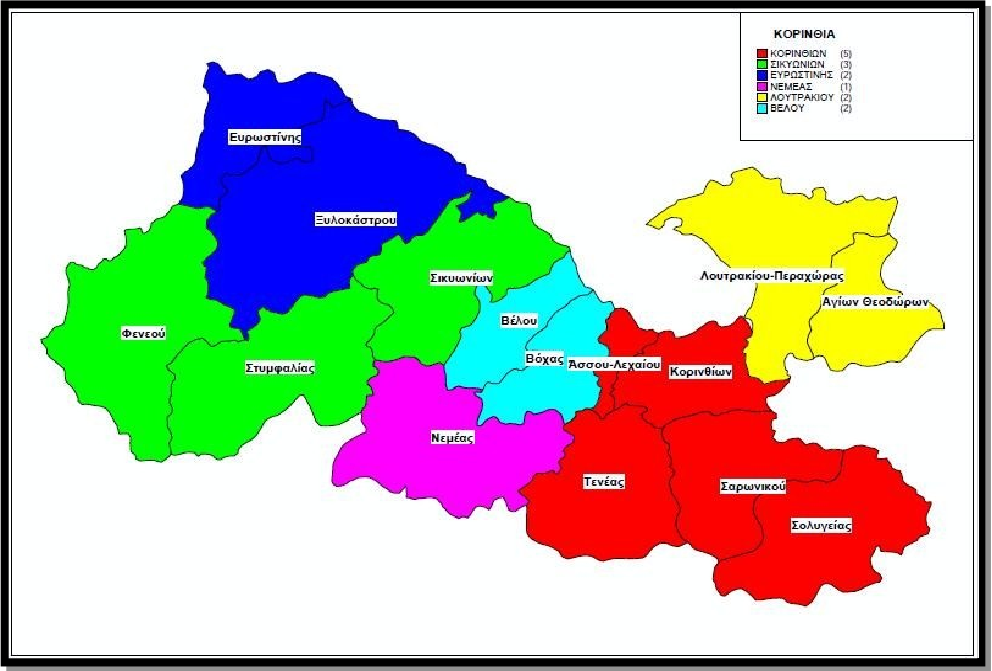
\includegraphics [scale = 0.55] {korinthia.png}
			\caption{Δήμοι Καλλικράτη Κορινθίας}
		\end{center}
	\end{figure}
	
	\textbf{Νομός Αργολίδας (Τέσσερις (4) Δήμοι) με έδρα το Ναύπλιο}
	\begin{itemize}
		\item \emph{Δήμος Άργους-Μυκηνών} με έδρα το Άργος (Συγχωνεύθηκαν οι Δήμοι Αλέας, Άργους, Αχλαδόκαμπου, Κουτσοποδίου, Λέρνας, Λυρκείας και Μυκηναίων)
		\item \emph{Δήμος Επιδαύρου} με έδρα το Ασκληπιείο Επιδαύρου (Συγχωνεύθηκαν οι Δήμοι Ασκληπιείου και Επιδαύρου)
		\item \emph{Δήμος Ερμιονίδας} με έδρα το Κρανίδι (Συγχωνεύθηκαν οι Δήμοι Ερμιόνης και Κρανιδίου)
		\item \emph{ήμος Ναυπλιέων} με έδρα το Ναύπλιο (Συγχωνεύθηκαν οι Δήμοι Ασίνης, Μιδέας, Ναυπλιέων και Νέας Τίρυνθας)
	\end{itemize}

	\begin{figure} [H]
		\begin{center}
			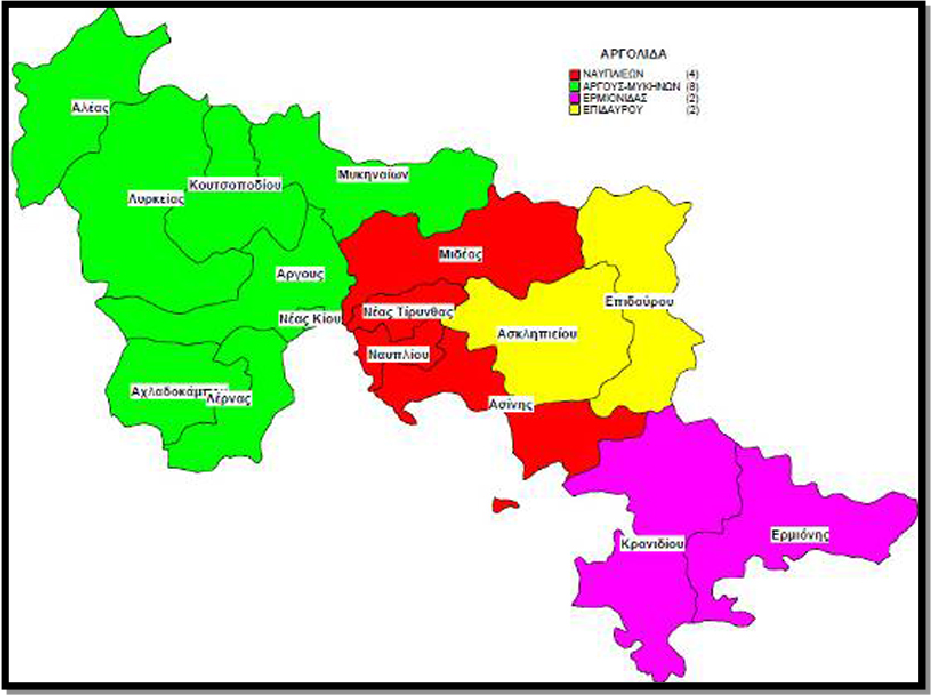
\includegraphics [scale = 0.60] {argolida.png}
			\caption{Δήμοι Καλλικράτη Αργολίδας}
		\end{center}
	\end{figure}

	\textbf{Νομός Αρκαδίας (Πέντε (5) Δήμοι) με έδρα την Τρίπολη)}
	\begin{itemize}
		\item \emph{Δήμος Βόρειας Κυνουρίας} με έδρα το Άστρος (Δεν υπήρξε κάποια μεταβολή)
		\item \emph{Δήμος Γορτυνίας} με έδρα τη Δημητσάνα (Συγχωνεύθηκαν οι Δήμοι Βυτίνας, Δημητσάνης, Ηραίας, Κλείτορος, Κοντοβαζαίνης, Λαγκαδίων, Τρικολώνων και Τροπαίων)
		\item \emph{Δήμος Μεγαλόπολης} με έδρα τη Μεγαλόπολη (Συγχωνεύθηκαν οι Δήμοι Γόρτυνος, Μεγαλόπολης και Φαλαισίας)
		\item \emph{Δήμος Κυνουρίας} με έδρα το Λεωνίδιο (Συγχωνεύθηκαν οι Δήμοι Κοσμά, Λεωνιδίου και Τυρού)
		\item \emph{Δήμος Τριπόλεως} με έδρα την Τρίπολη (Συγχωνεύθηκαν οι Δήμοι Βαλτετσίου, Κορυθίου, Λεβιδίου, Μαντινείας, Σκιριτίδας, Τεγέας, Τρίπολης και Φαλάνθου)
	\end{itemize}

	\begin{figure} [H]
		\begin{center}
			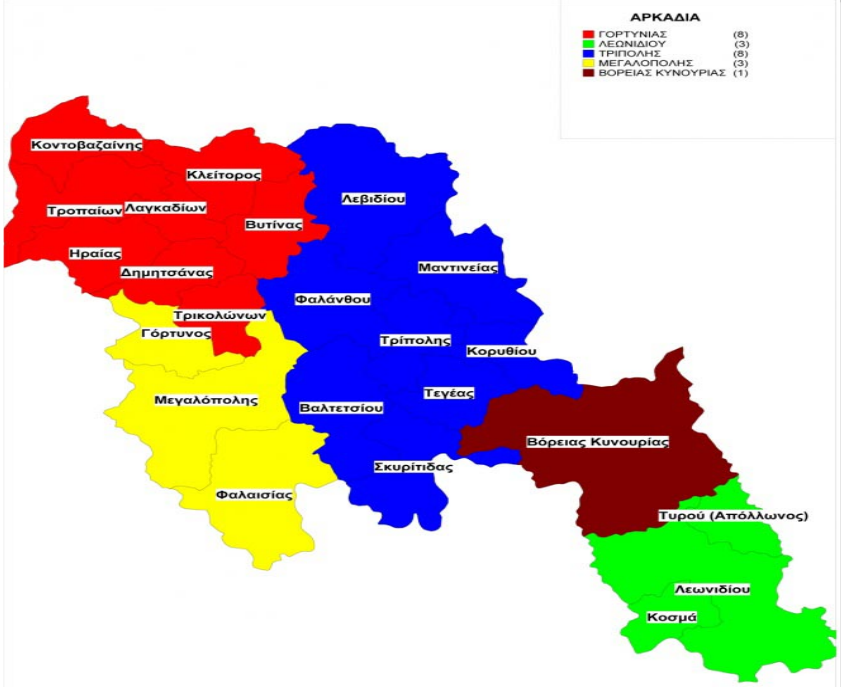
\includegraphics [scale = 0.60] {arkadia.png}
			\caption{Δήμοι Καλλικράτη Αρκαδίας}
		\end{center}
	\end{figure}

	\textbf{Νομός Μεσσηνίας (έξι(6) Δήμοι) με έδρα την Καλαμάτα}
	\begin{itemize}
		\item \emph{Δήμος Δυτικής Μάνης} με έδρα την Καρδαμύλη (Συγχωνεύθηκαν οι Δήμοι Αβίας και Λεύκτρου)
		\item \emph{Δήμος Καλαμάτας} με έδρα την Καλαμάτα (Συγχωνεύθηκαν οι Δήμοι Αρίου, Αρφαρών, Θουρίας και Καλαμάτας)
		\item \emph{Δήμος Μεσσήνης} με έδρα τη Μεσσήνη (Συγχωνεύθηκαν οι Δήμοι Αιπείας, Ανδρούσας, Αριστομένους, Βουφράδων, Ιθώμης, Μεσσήνης, Πεταλιδίου και η κοινότητα Τρικόρφου)
		\item \emph{Δήμος Οιχαλίας} με έδρα το Μελιγαλά (Συγχωνεύθηκαν οι Δήμοι Ανδανίας, Δωρίου, Είρας, Μελιγαλά και Οιχαλίας)
		\item \emph{Δήμος Πύλου-Νέστορος} με έδρα την Πύλο (Συγχωνεύθηκαν οι Δήμοι Κορώνης, Μεθώνης, Παπαφλέσσα, Πύλου, Νέστορος και Χιλιοχωρίων)
		\item \emph{Δήμος Τριφυλλίας} με έδρα την Κυπαρισσία (Συγχωνεύθηκαν οι Δήμοι Αετού, Αυλώνος, Γαργαλιάνων, Κυπαρισσίας, Φιλιατρών και η κοινότητα Τριπύλας)
	\end{itemize}

	\begin{figure} [H]
		\begin{center}
			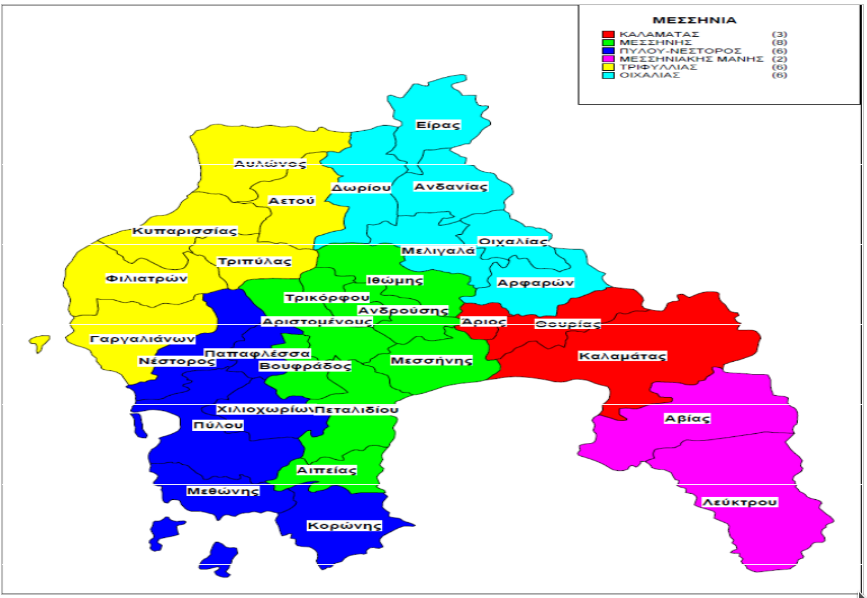
\includegraphics [scale = 0.60] {messinia.png}
			\caption{Δήμοι Καλλικράτη Μεσσηνίας}
		\end{center}
	\end{figure}

	\textbf{Νομός Λακωνίας (Πέντε (5) Δήμοι) με έδρα τη Σπάρτη}
	
	\begin{itemize}
		\item \emph{Δήμος Ανατολικής Μάνης} με έδρα το Γύθειο (Συγχωνεύθηκαν οι Δήμοι Ανατολικής Μάνης, Γυθείου, Οιτύλου και Σμύνους)
		\item \emph{Δήμος Ελαφονήσου} με έδρα την Ελαφόνησο (Δεν υπήρξε κάποια μεταβολή)
		\item \emph{Δήμος Ευρώτα} με έδρα τη Σκάλα (Συγχωνεύθηκαν οι Δήμοι Γερόνθρων, Έλους, Κροκεών, Νιάτων και Σκάλας)
		\item \emph{Δήμος Μονεμβασιάς} με έδρα τους Μολάους (Συγχωνεύθηκαν οι Δήμοι Ασωπού, Βοιών, Ζαράκα, Μολάων και Μονεμβασιάς)
		\item \emph{Δήμος Σπάρτης} με έδρα τη Σπάρτη (Συγχωνεύθηκαν οι Δήμοι Θεραπνών, Καρυών, Μυστρά, Οινούντος, Πελλάνας, Σπαρτιατών και Φαρίδος)
	\end{itemize}

	\begin{figure} [H]
		\begin{center}
			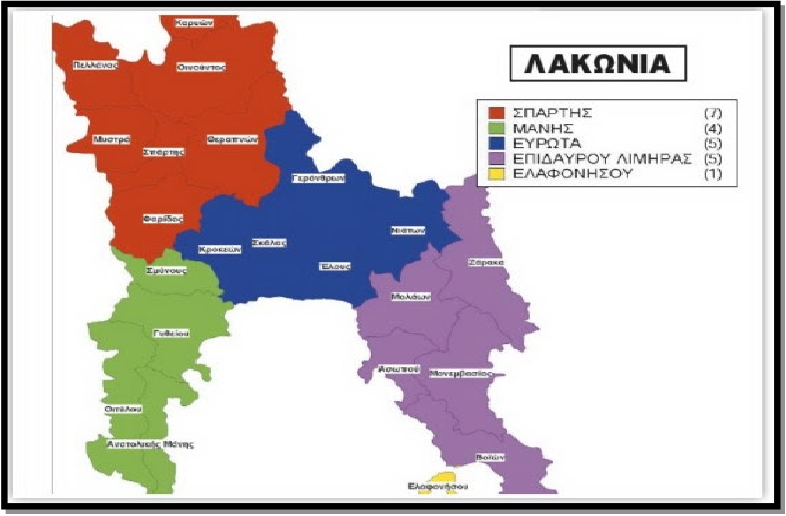
\includegraphics [scale = 0.60] {lakonia.png}
			\caption{Δήμοι Καλλικράτη Λακωνίας}
		\end{center}
	\end{figure}
	
	\subsubsection{Φυσικό περιβάλλον}
	
	\paragraph{Ανάγλυφο}
	
	\textbf{Γεωγραφία} 
	
	Η Περιφέρεια Πελοποννήσου αποτελεί το νοτιότερο τμήμα της ηπειρωτικής Ελλάδας καλύπτει το 11,7\% της συνολικής έκτασης της χώρας. Καταλαμβάνει ένα μέρος του βόρειου τμήματος, ολόκληρο το νοτιοανατολικό και ένα μέρος του δυτικού τμήματος του συνόλου της Πελοποννήσου και συνορεύει δυτικά με την Περιφέρεια Δυτικής Ελλάδας, και βορειοανατολικά με την Περιφέρεια Αττικής. Οι νομοί που βρίσκονται στο έδαφός της είναι οι νομοί Κορινθίας, Αργολίδας, Αρκαδίας, Μεσσηνίας και Λακωνίας. Το έδαφος της Περιφέρειας Πελοποννήσου είναι κατά κύριο λόγο ορεινό ιδίως στα κεντρικά  και τα ανατολικά με τους ορεινούς όγκους να καταλαμβάνουν περίπου τη μισή έκτασή της συγκεκριμένα το 50,1\%, ωστόσο στα βόρεια στα δυτικά και στα νότια της Περιφέρειας βρίσκονται μερικές από τις πιο εύφορες πεδινές εκτάσεις της Ελλάδας (συνολικά αποτελούν το 19,9\% της έκτασής της) στις παραθαλάσσιες κυρίως περιοχές, όπως ο Αργολικός και ο Κορινθιακός Κάμπος.
	
	\begin{figure} [H]
		\begin{center}
			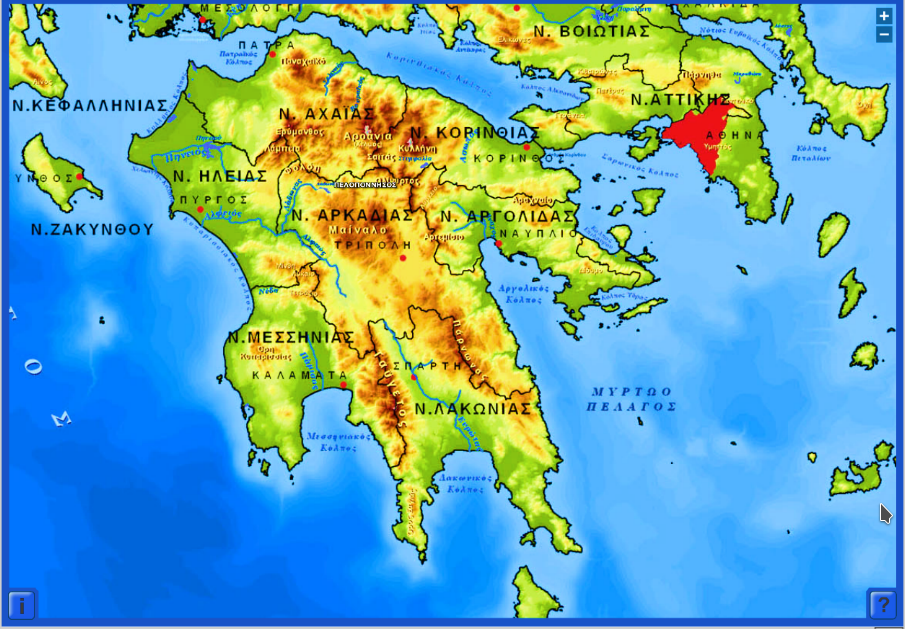
\includegraphics [scale = 0.60] {peloponnisos.png}
		\end{center}
	\caption{Γεωμορφολογικός χάρτης Πελοποννήσου}
	\label{peloponnese}
	\end{figure}

	Τα σημαντικότερα \emph{όρη} της Περιφέρειας είναι ο Ταΰγετος (2406μ) που βρίσκεται στα σύνορα των νομών Μεσσηνίας και Λακωνίας, η Κυλλήνη (2380μ) στο νομό Κορινθίας, το Μαίναλο (1980μ) στο νομό Αρκαδίας, ο Πάρνωνας (1935μ) που μοιράζεται μεταξύ των νομών Αρκαδίας και Λακωνίας, καθώς και ο Ολίγυρτος (1934μ) που βρίσκεται βορειοανατολικά του Μαινάλου στο νομό Αρκαδίας. Βέβαια στο έδαφος της Περιφέρειας υπάρχει πληθώρα άλλων οροσειρών μικρότερου ύψους.
	
	Οι υδροκρίτες των ορεινών όγκων σε συνδυασμό με τις αρκετά έντονες βροχοπτώσεις κυρίως στα κεντρικά και τα δυτικά της Περιφέρειας παράγουν πλήθος υδατορευμάτων και ποταμών που διασχίζουν το έδαφός της και εκβάλλουν σε κάποιο από τα Πελάγη τα οποία την περιβάλλουν. Οι πιο σημαντικοί \emph{ποταμοί} είναι ο Αλφειός, που πηγάζει από τα οροπέδια της Μεγαλόπολης, διασχίζει τους νομούς Αρκαδίας και Ηλείας και εκβάλλει στον κόλπο της Κυπαρισσίας, ο Ευρώτας, ο οποίος έχει τις πηγές του επίσης στα οροπέδια της Μεγαλόπολης και αφού διασχίσει το νομό Λακωνίας εκβάλλει στο Λακωνικό κόλπο. Άλλοι μικρότεροι ποταμοί είναι ο Λάδωνας, που πηγάζει από καρστικές πηγές στο νομό Αχαΐας και περνώντας από το νομό Αρκαδίας ενώνεται με τον Αλφειό αποτελώντας στην ουσία παραπόταμο αυτού, καθώς και οι ποταμοί Πάμισος και Νέδων, που πηγάζουν από τον Ταΰγετο και καταλήγουν στο Μεσσηνιακό κόλπο. Τέλος, ο ποταμός Νέδα πηγάζει από το όρος Λύκαιο και χύνεται στον κόλπο Κυπαρισσίας διασχίζοντας τα σύνορα των νομών Ηλείας και Μεσσηνίας.  
	
	Αξιόλογες \emph{λίμνες} δεν υπάρχουν στην Πελοπόννησο. Υπάρχουσες σήμερα λίμνες είναι η Τάκα στο νομό Αρκαδίας, η Στυμφαλία στο νομό Κορινθίας, η τεχνητή του Λάδωνα στο νομό Αρκαδίας που δημιουργήθηκε με την κατασκευή των υδροηλεκτρικών έργων, η λίμνη Δόξα στο νομό Αρκαδίας επίσης τεχνητή λίμνη σε υψόμετρο 900 μέτρων.
	
	Παρά το γενικά ορεινό έδαφος η Περιφέρεια έχει κάποιες αξιόλογες \emph{πεδιάδες}. Στα δυτικά των βουνών της Κυπαρισσίας απλώνεται η στενή παραλιακή πεδιάδα της Κυπαρισσίας-Γαργαλιάνων. Στο ΝΔ τμήμα της Πελοποννήσου εκτείνεται η πεδιάδα της Μεσσηνίας. Στην Ανατολική Πελοπόννησο υπάρχουν, στο Β. μέρος η Αργολική πεδιάδα, η οποία απλώνεται ως την πεδιάδα του Κρανιδίου και στο νότιο τμήμα η πεδιάδα του Έλους, η οποία προς τα Β. συνεχίζεται με την κοιλάδα του Ευρώτα και προς Ν. με τις παραλιακές πεδιάδες Ασωπού και Νεάπολης Βοιών. Στα βόρεια της Πελοποννήσου υπάρχει μια στενή παραλιακή πεδιάδα, η οποία φέρει διάφορες τοπικές ονομασίες, όπως πεδιάδα της Βόχας, του Αιγίου, Σικυώνιο Πεδίο κλπ.
	
	Εκτός από τις πεδιάδες υπάρχουν και αξιόλογα \emph{οροπέδια}. Αυτά είναι οι λεκάνες της Μαντινείας, Τεγέας και Ασέας. Και τα δύο μαζί ονομάζονται Οροπέδιο της Τρίπολης. Δυτικά από αυτό το οροπέδιο βρίσκεται το οροπέδιο της Μεγαλόπολης. Επίσης μεταξύ Αροανίων και Κυλλήνης υπάρχουν τα μικρά οροπέδια του Φενεού και της Στυμφαλίας.
	
	\textbf{Ακτογραφία}
	
	Όλοι οι νομοί της Περιφέρειας βρέχονται από θάλασσα στο μεγαλύτερο μέρος της περιμέτρου τους με εξαίρεση το νομό Αρκαδίας, που ένα πολύ μικρό κομμάτι του διαβρέχεται από τον Αργολικό Κόλπο στα ανατολικά. Η ακτογραμμή που περιβάλλει την Περιφέρεια παρουσιάζει ποικιλία ανωμαλιών και επικοινωνεί στα δυτικά με το Ιόνιο Πέλαγος, στα ανατολικά με το Αιγαίο Πέλαγος και στα νότια με το Κρητικό Πέλαγος και τη Μεσόγειο Θάλασσα. Οι βασικότεροι κόλποι που σχηματίζει η ακτογραμμή είναι ο Μεσσηνιακός, ο Λακωνικός, ο Αργολικός, ο Σαρωνικός και ο Κορινθιακός, καθώς και ο κόλπος της Κυπαρισσίας.
	
	\paragraph{Έδαφος-Γεωλογία-Υδατικοί Πόροι}
	
	\textbf{Έδαφος}
	
	Το έδαφος της Πελοποννήσου απειλείται κυρίως από δυο φαινόμενα την απερήμωση και τη διάβρωση των ακτών. Απερήμωση ή ερημοποίηση είναι η διαδικασία της μετατροπής γόνιμων γαιών σε εκτάσεις ερήμου, τυπικά ως αποτέλεσμα αποδασώσεως, ξηρασίας ή λανθασμένων/ακατάλληλων γεωργικών ή κτηνοτροφικών μεθόδων». Εξάλλου, η ερημοποίηση έχει επαρκώς οριστεί στο κείμενο της Συμβάσεως των Ηνωμένων Εθνών για την Καταπολέμηση της Ερημοποιήσεως (UNCCD) ως «υποβάθμιση γαιών σε ξηρές, ημίξηρες και μικρής υγρασίας περιοχές που προκαλείται από διάφορους παράγοντες, όπως οι κλιματικές μεταβολές και οι ανθρώπινες δραστηριότητες». Το φαινόμενο αυτό έχει ως αποτέλεσμα όπως αναφέρθηκε τη μείωση της παραγωγικότητας του εδάφους καθώς και τη μείωση της ποιότητας και της ποσότητας των υδατικών πόρων.
	Όπως φαίνεται στο χάρτη δυνητικού κινδύνου ερημοποίησης της Ελλάδας που συνετάχθη από την Εθνική Επιτροπή κατά της Ερημοποίησης στην Περιφέρεια Πελοποννήσου υπάρχουν ελάχιστες ζώνες χαμηλού κινδύνου, ενώ ως επί το πλείστον υπάρχουν ζώνες μέτριου έως υψηλού κινδύνου λόγω διάβρωσης. Αναλυτικά οι ζώνες υψηλού κινδύνου βρίσκονται στους νομούς Λακωνίας, Αρκαδίας, Αργολίδας και σε πολύ μικρή έκταση του νομού Μεσσηνίας, ενώ οι ζώνες μέτριου κινδύνου στους νομούς Κορινθίας Μεσσηνίας και εν μέρει Λακωνίας.
	
	\begin{figure} [H]
		\begin{center}
			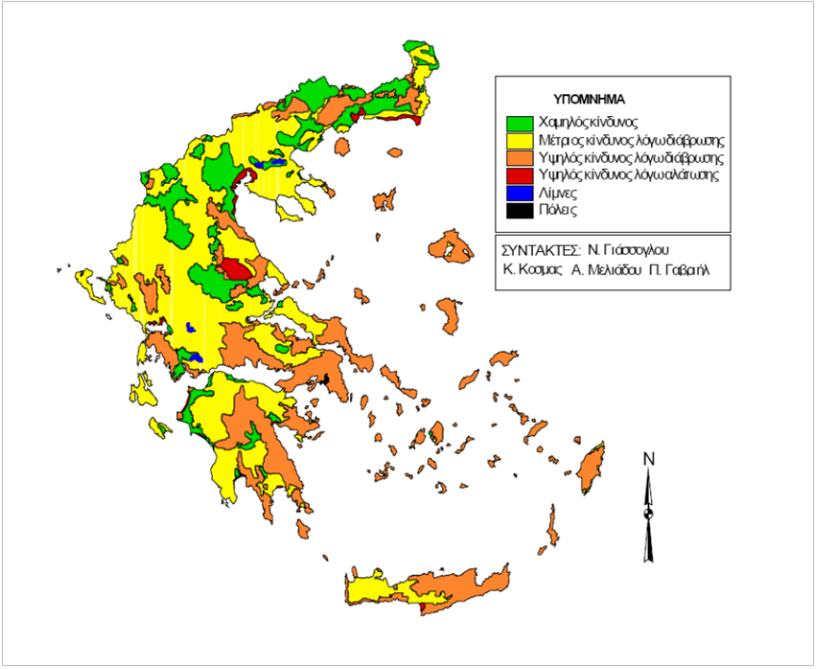
\includegraphics [scale = 0.60] {erimopoiisi.png}
			\caption{Χάρτης δυνητικού κινδύνου ερημοποίησης της Ελλάδας}
			\label{erimopoiisi}
		\end{center}
	\end{figure}

	Σύμφωνα με την ταξινόμηση των εδαφών, βάσει του συστήματος FAO (Χάρτης Εδαφών Ελλάδας – Εθνική Επιτροπή κατά της Ερημοποίησης – Γεωπονικό Πανεπιστήμιο Αθηνών – Συντάκτης Ν. Γιάσογλου – ( Παράρτημα IΙ ), τα εδάφη της Περιφέρειας Πελοποννήσου ταξινομούνται σε επτά κατηγορίες εδαφών, οι οποίες είναι:

	\begin{itemize}
		\item \emph{Βράχοι}(Rock Outcrops) (μαύρο χρώμα)
		\item \emph{\selectlanguage{english}Leptosols}\selectlanguage{english}(LP): \selectlanguage{greek}Εδάφη με μητρικό υλικό από ασβεστόλιθο και φλύσχη. Είναι λεπτόκοκκα εδάφη, αργιλώδη, καλής υδατοπερατότητας με ουδέτερο \selectlanguage{english}pH. \selectlanguage{greek}(γκρι χρώμα)
		\item \emph{\selectlanguage{english}Regosols}\selectlanguage{english}(RG): \selectlanguage{greek}Στρώμα χαλαρού υλικού, πάνω σε σκληρό υπόβαθρο. Είναι εδάφη μετρίως αργιλώδη, με μέτρια υδατοπερατότητα και με \selectlanguage{english}pH $>$ 7.\selectlanguage{greek}(κίτρινο χρώμα)
		\item \emph{\selectlanguage{english}Fluvisols}\selectlanguage{english}(FL): \selectlanguage{greek}Εδάφη αργιλώδη, με μέτρια έως μικρή υδατοπερατότητα και με \selectlanguage{english}pH $>$ 7.\selectlanguage{greek}(μπλε χρώμα)
		\item \emph{\selectlanguage{english}Cambisols}\selectlanguage{english}(CM): \selectlanguage{greek}Η σύσταση των εδαφών αυτών είναι αργιλλώδης και μετρίως αργιλλώδης, με μικρή υδατοπερατότητα και με ουδέτερο ή ελαφρώς όξινο \selectlanguage{english}pH. \selectlanguage{greek}(πορτοκαλί χρώμα)
		\item \emph{\selectlanguage{english}Luvisols}\selectlanguage{english}(LV): \selectlanguage{greek}Τα εδάφη αυτά είναι αργιλώδη με υψηλή υδατοπερατότητα και με \selectlanguage{english}pH $\approx$ 7.\selectlanguage{greek}(ροζ χρώμα)
	\end{itemize}

	\begin{figure} [H]
		\begin{center}
			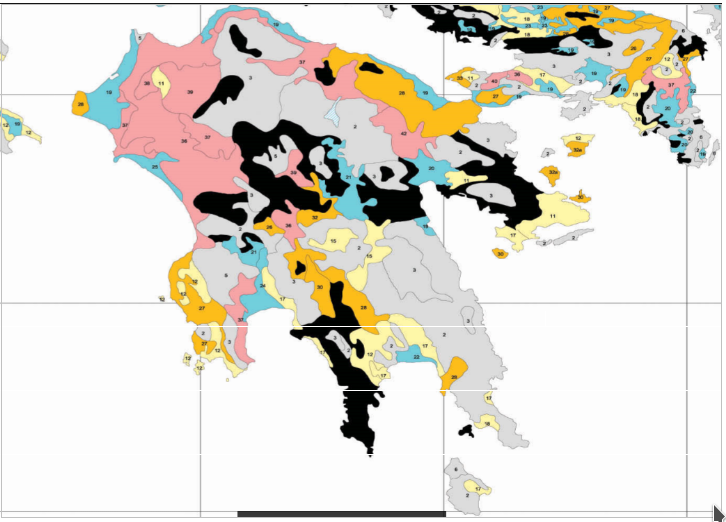
\includegraphics [scale = 0.70] {edafi.png}
			\caption{Ταξινόμηση εδαφών Πελοποννήσου}
			\label{edafi}
		\end{center}
	\end{figure}
	
	\textbf {\underline{Γεωλογία-Τεκτονική: Γεωτεκτονικές ζώνες Πελοποννήσου}}
	
	Όπως φαίνεται και στο σχήμα γεωτεκτονικών ενοτήτων Ελλάδος στην Περιφέρεια Πελοποννήσου εμφανίζονται έξι γεωτεκτονικές ζώνες (ζώνη Παρνασσού Γκιώνας, ζώνη Γαβρόβου-Τριπόλεως, Πελαγονική ζώνη, ζώνη Παξών, ζώνη Ιόνιος και ζώνη Ολωνού-Πίνδου) το σύμπλεγμα των οφιολίθων και οι σχηματισμοί του προαλπικού υποβάθρου.
	
	\textbf{Ζώνη Παρνασσού-Γκιώνας}
	
	Η ζώνη αυτή έχει περιορισμένη έκταση στην Κεντρική Ελλάδα και αποτελείται σχεδόν αποκλειστικά από ασβεστόλιθους και δολομίτες, με βασικό χαρακτηριστικό την ύπαρξη τριών  βοξιτικών οριζόντων. (Σημειώνεται ότι οι βωξίτες αποτελούσαν για δεκαετίες σημαντικό παράγοντα για την οικονομία της χώρας). Απουσιάζουν εντελώς τα μαγματικά πετρώματα. Βρίσκεται απωθημένη προς τα δυτικά πάνω στη ζώνη της Πίνδου.
	
	\textbf{Ζώνη Ολωνού-Πίνδου}
	
	Κατέχει κεντρική θέση στον κορμό της Ελλάδας και ακολουθεί την κάμψη του ορογενετικού τόξου, ενώ τμήματα της απαντούν στην Κρήτη και τη Ρόδο. Συνίσταται από ασβεστόλιθους, δολομίτες, κερατόλιθους, ηφαιστειοϊζηματογενή πετρώματα, ραδιολαρίτες, αργίλους, ψαμμίτες και πηλίτες. Έχει επωθηθεί προς τα δυτικά πάνω στη ζώνη Γαβρόβου-Τριπόλεως και χαρακτηρίζεται από δομή λεπίων, με αποτέλεσμα συχνές επαναλήψεις των στρωμάτων. Πάνω στη ζώνη της Πίνδου βρίσκονται επωθημένες οι μεγαλύτερες οφιολιθικές μάζες του ελληνικού χώρου.
	
	\textbf{Ζώνη Γαβρόβου-Τριπόλεως}
	
	Η ζώνη Γαβρόβου - Τριπόλεως χαρακτηρίζεται από συνεχή ανθρακική ιζηματογένεση με κυρίαρχα πετρώματα τους ασβεστόλιθους και δολομίτες. Οι σχηματισμοί της ζώνης αυτής επικάθονται σε ένα υπόβαθρο αποτελούμενο από φυλλίτες, χαλαζιακούς φυλλίτες και μάρμαρα, γνωστό ως «φυλλιτική-χαλαζιτική» σειρά. Τα στρώματά της σχηματίζουν μεγάλα ανοικτά σύγκλινα και αντίκλινα και είναι επωθημένη δυτικά πάνω στην Ιόνιο ζώνη.
	
	\textbf{Ιόνιος (ή Αδριατικοϊόνιος) ζώνη}
	
	Χαρακτηρίζεται από την παρουσία εβαποριτών, κυρίως γύψου και ορυκτού άλατος, στη βάση της αλλά και σε ανώτερα στρώματα, όπου ανήλθαν λόγω διαπυρισμού. (Σημειώνεται ότι οι εβαπορίτες παρουσιάζουν μεγάλο ενδιαφέρον στην έρευνα πετρελαίων). Ακολουθεί μια σχεδόν  συνεχής ιζηματογένεση όπου επικρατούν οι ασβεστόλιθοι, πελαγικοί και νηριτικοί, δολομίτες, αργιλικοί σχιστόλιθοι και κερατόλιθοι. Είναι επωθημένη προς τα δυτικά πάνω στη ζώνη Παξών. Με την Ιόνιο ζώνη (θεωρούμενη ως η προς νότο η μεταμορφωμένη συνέχεια της) σχετίζεται μια σειρά πλακωδών μαρμάρων με διαστρώσεις πυριτολίθων, γνωστή  ως σειρά των Plattenkalk (Πλακώδεις ασβεστόλιθοι) που απαντούν σε μεγάλη έκταση στην Πελοπόννησο και Κρήτη.
	
	\textbf{Ζώνη Παξών (ή Προαπούλια)}
	
	Είναι η  πιο εξωτερική γεωτεκτονική ζώνη της Ελλάδας, της οποίας εμφανίζεται  ένα μικρό τμήμα στα Ιόνια νησιά και ένα στη νότια Πελοπόννησο. Χαρακτηρίζεται από μια συνεχή νηριτική ιζηματογένεση και την απουσία φλύσχη.  Τα παλαιότερα πετρώματα είναι γύψοι και ακολουθούν δολομίτες, ασβεστόλιθοι, μαργαϊκοί ασβεστόλιθοι, μάργες και κερατόλιθοι. Θεωρείται ως αυτόχθονη ζώνη, το μεγαλύτερο τμήμα της οποίας είναι βυθισμένο στη θάλασσα, μεταξύ των ιόνιων νησιών και της Απουλίας (στην Νότιο Ιταλία).
	
	\textbf{Πελαγονική Ζώνη}
	
	Η Πελαγονική ζώνη κατέχει ένα μεγάλο τμήμα του κορμού της Ελλάδας και αποτελείται από ένα κρυσταλλοσχιστώσες υπόβαθρο (γνεύσιους, γνευσιοσχιστόλιθους και  αμφιβολίτες με μεγάλες γρανιτικές διεισδύσεις), μάρμαρα, φυλλίτες, σχιστόλιθους, ψαμμίτες, ασβεστόλιθους και δολομίτες. Χαρακτηριστική είναι η ύπαρξη τεκτονικά τοποθετημένων μεγάλων οφιολιθικών μαζών. Διακρίνεται στην Πελαγονική ζώνη  μεταμορφωμένων σχηματισμών (όπου εμφανίζονται αποκλειστικά μεταμορφωμένα πετρώματα) και την Πελαγονική ζώνη μη μεταμορφωμένων σχηματισμών (ή Υποπελαγονική).
	
	\begin{figure} [H]
		\begin{center}
			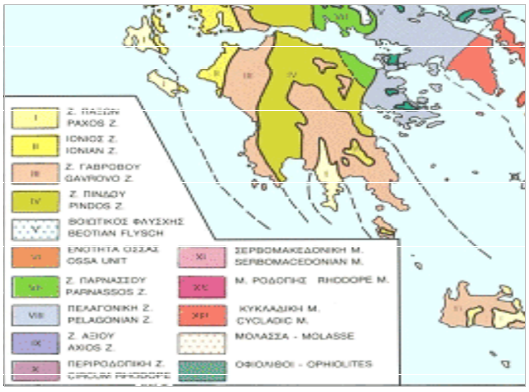
\includegraphics [scale = 0.75] {geotektonikes.png}
			\caption{Γεωτεκτονικές ζώνες Πελοποννήσου}
			\label{geotektonikes}
		\end{center}
	\end{figure}

	\textbf{\underline{Υδατικοί Πόροι}}
	
	Ο υδατικός τομέας της Πελοποννήσου παρουσιάζει εκτεταμένα προβλήματα κυρίως λόγω της υπεράντλησης για την άρδευση των γεωργικών εκτάσεων οι οποίες καλύπτουν μεγάλο μέρος της επιφάνειας της Πελοποννήσου. Σαν αποτέλεσμα αυτού παρατηρείται μόλυνση και υφαλμύρωση του υπόγειου υδροφορέα με επικίνδυνες συνέπειες τόσο για τις καλλιέργειες όσο και για την υγεία των κατοίκων.
	
	Η Περιφέρεια Πελοποννήσου διαιρείται σε τρία υδατικά διαμερίσματα, όπως φαίνεται και στον παρακάτω χάρτη.
	
	\begin{figure} [H]
		\begin{center}
			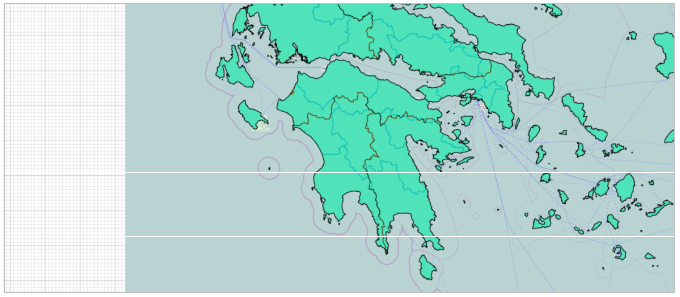
\includegraphics [scale = 0.75] {ydatika.png}
			\caption{Υδατικά διαμερίσματα Πελοποννήσου}
			\label{ydatika}
		\end{center}
	\end{figure}

	Το Υδατικό Διαμέρισμα της βόρειας Πελοποννήσου περιλαμβάνει το βόρειο τμήμα του νομού Ηλείας το μεγαλύτερο μέρος του νομού Αχαΐας, εξ ολοκλήρου το νομό Κορινθίας και ελάχιστο μέρος του νομού Αργολίδας και έχει έκταση 6107,48τ.χλμ. Ο υδροκρίτης του υδατικού διαμερίσματος ξεκινά από το όρος Ερύμανθος στο νομό Αχαΐας και συνεχίζει μέχρι τα Αροάνεια Όρη του νομού Αχαΐας και το όρος Κυλλήνη στο νομό Κορινθίας και αφού ενωθεί με τον υδροκρίτη των οροσειρών Ολιγύρτου, Τραχέως και Λυρκείου του νομού Αρκαδίας καταλήγει στο όρος Αραχναίο στο νομό Αργολίδας.
	
	Το Υδατικό Διαμέρισμα της Δυτικής Πελοποννήσου περιλαμβάνει το νότιο τμήμα του νομού Ηλείας, περίπου το ήμισυ του νομού Αρκαδίας και εξ ολοκλήρου το νομό Μεσσηνίας και έχει έκταση 7205,43τ.χλμ. Ο υδροκρίτης του υδατικού διαμερίσματος ξεκινά από το όρος Μαίναλο του νομού Αρκαδίας και αφού ενωθεί με τους υδροκρίτες της οροσειράς της Κυπαρισσίας καθώς και του Λυκαίου και του Τετραζίου στο νομό Μεσσηνίας καταλήγει στον Ταΰγετο.
	
	Το Υδατικό Διαμέρισμα της ανατολικής Πελοποννήσου αποτελείται από το ήμισυ του νομού Αρκαδίας και πρακτικά το σύνολο των νομών Αργολίδας και Λακωνίας και έχει έκταση 8007,42τ.χλμ. Ο υδροκρίτης του υδατικού διαμερίσματος ξεκινά από το όρος Δίδυμο συνεχίζει στο όρος Αραχναίο και αφού περάσει από τα όρη Ολίγυρτος Τραχύ, Λύρκειο και Αρτεμίσιο διακλαδώνεται στους υδροκρίτες των βουνών Ταΰγετος και Πάρνωνας.
	
	Γενικά παρά το έντονο ορεινό στοιχείο της Πελοποννήσου το έδαφός της δεν διαβρέχουν μεγάλοι ποταμοί.\\
	Πιο αναλυτικά:
	
	Στον  Κορινθιακό κόλπο εκβάλλει ο ποταμός Ασωπός ο οποίος πηγάζει από το όρος Τραχύ καθώς και το ρέμα Φόνισσα στην περιοχή του Καμαρίου.
	
	Στον Αργολικό κόλπο εκβάλουν οι ποταμοί Τάνος, Ερασίνος (Κεφαλάρι) και ο Ίναχος που πηγάζει από τα βουνά Λύρκειο και Τραχύ.
	
	Στο νομό Αρκαδίας και συγκεκριμένα από το οροπέδιο της Τρίπολης πηγάζουν οι ποταμοί Αλφειός, Λάδωνας και Ερύμανθος και στα σύνορα με την Ηλεία οι δύο τελευταίοι ενώνονται με τον Αλφειό και εκβάλλουν στον κόλπο της Κυπαρισσίας. Η υδρολογική λεκάνη του Αλφειού έχει επιφάνεια έκτασης 3809,9 τ.χλμ. και καλύπτει μέρος των νομών Αρκαδιός, Ηλείας και Αχαΐας.
	
	Στο νομό Μεσσηνίας από τον Ταΰγετο πηγάζουν οι ποταμοί Νέδων και Πάμισος (μήκους 48χλμ.) που χύνονται στον Μεσσηνιακό κόλπο ανάμεσα στις πόλεις Μεσσήνη και Καλαμάτα . Στην ίδια περιοχή χύνεται και ο ποταμός Βελίκας που πηγάζει από τα βουνά της Κυπαρισσίας. Επίσης από το όρος Λύρκειο πηγάζει ο ποταμός Νέδα μήκους 32χλμ που εκβάλλει στον κόλπο της Κυπαρισσίας.
	
	Τέλος στο νομό Λακωνίας υπάρχει ένας και μοναδικός ποταμός, ο Ευρώτας, που πηγάζει από το αρκαδικό οροπέδιο, νότια της Μαντινείας. Μετά από μία διαδρομή 82 χλμ., στην κοιλάδα που ορίζουν ο Πάρνωνας και ο Ταΰγετος, κατά τη διάρκεια της οποίας δέχεται τα νερά από αρκετούς παραποτάμους, εκβάλλει στο μυχό του Λακωνικού Κόλπου, σχηματίζοντας δέλτα. 
	
	Ως προς τις λίμνες η Πελοπόννησος δεν έχει να αναδείξει σημαντικές ποσότητες. Στο νομό Κορινθίας υπάρχουν η λιμνοθάλασσα της Βουλιαγμένης και η λίμνη Στυμφαλία καθώς και η τεχνητή λίμνη Φενεού. Η Λίμνη Βουλιαγμένη βρίσκεται 16 χιλιόμετρα βορειοδυτικά του Λουτρακίου, πολύ κοντά στην περιοχή του αρχαιολογικού χώρου του Ηραίου και στον οικισμό Περαχώρα. Έχει μέγιστο μήκος 2 χλμ. και μέγιστο πλάτος περίπου 1 χλμ. Το βάθος της δεν υπερβαίνει τα 40 μέτρα. Διαθέτει παραλία με άμμο εν αντιθέσει με την παραλία του Λουτρακίου. Επικοινωνεί με τα νερά του Κορινθιακού κόλπου από ένα πολύ στενό κανάλι που το πλάτος του δεν υπερβαίνει τα 6 μέτρα. Η Στυμφαλία είναι ελώδης λίμνη της ορεινής Κορινθίας. Βρίσκεται σε ένα οροπέδιο σε υψόμετρο 600 μέτρων ανάμεσα στα όρη Κυλλήνη και Ολίγυρτος. Διατηρεί νερό κυρίως τους χειμερινούς μήνες και η έκτασή της φτάνει τα 3,5 τ.χλμ. Το βάθος της Λίμνης στα σημεία οπού καλύπτεται μονίμως από νερό κυμαίνεται από 2-2,5 μέτρα την Άνοιξη και μισό (0,5) περίπου μέτρο στις αρχές του Φθινοπώρου.
	
	Στο νομό Αρκαδίας υπάρχουν η λίμνη Τάκα και η τεχνητή λίμνη του Λάδωνα. Η λίμνη Τάκα βρίσκεται σε υψόμετρο 650 μέτρα στο οροπέδιο της Τεγέας και σε απόσταση 10 χιλιόμετρα από την Τρίπολη. Έχει γλυκό νερό και αποτελεί σημαντικό υδροβιότοπο της Πελοποννήσου με πολλά πτηνά και ψάρια. Η λίμνη Τάκα αποτελεί κυρίως εποχιακή λίμνη και αποστραγγίζεται μέσα από ένα σύστημα από καταβόθρες σε υπόγειους ποταμούς. Έτσι λοιπόν το καλοκαίρι αποστραγγίζεται ολοκληρωτικά, δημιουργώντας τέναγος. Το φθινόπωρο αρχίζει να γεμίζει πάλι, με μέγιστο βάθος το μισό μέτρο, με βρόχινα νερά αλλά και ρεμάτων που καταλήγουν στην λίμνη, ώσπου φτάνει σε πληρότητα κατά τη διάρκεια του χειμώνα. Ως αποτέλεσμα αυτής της διαδικασίας το χωριό Βουνό, στις όχθες της Τάκας, το χειμώνα είναι παρόχθιο και το καλοκαίρι μεσόγειο. Ανήκει στην λεκάνη απορροής του Αλφειού όπου μέσω των καταβόθρων τον εμπλουτίζει με τα νερά της. Η Λίμνη Λάδωνα είναι τεχνητή λίμνη που δημιουργήθηκε έπειτα από κατασκευή φράγματος στον ποταμό Λάδωνα. Αποτελεί τμήμα της λεκάνης απορροής του Αλφειού, παραπόταμος του οποίου είναι ο Λάδωνας. Η έκτασή της είναι 3,048 τ.χλμ.
	
	Η Περιφέρεια Πελοποννήσου έχει μεγάλες εκτάσεις υπογείων νερών κυρίως στο νομό Μεσσηνίας και στο ανατολικό τμήμα της, όπως φαίνεται στον παρακάτω χάρτη. 
	
	\begin{figure} [H]
		\begin{center}
			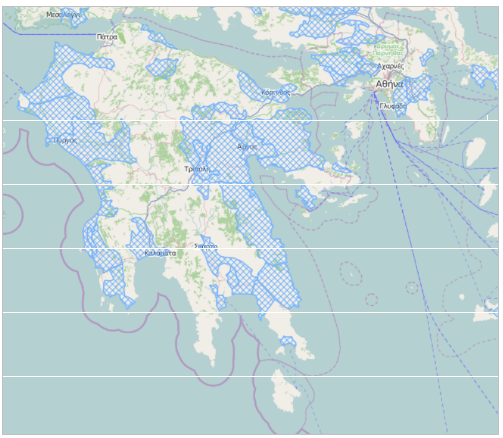
\includegraphics [scale = 0.75] {ypogeia.png}
			\caption{Υπόγεια νερά Πελοποννήσου}
			\label{ypogeia}
		\end{center}
	\end{figure}
	
	\paragraph{Στοιχεία σεισμικότητας-Σεισμική επικινδυνότητα-Κατολισθητική επικινδυνότητα}
	
	\begin{figure} [H]
		\begin{center}
			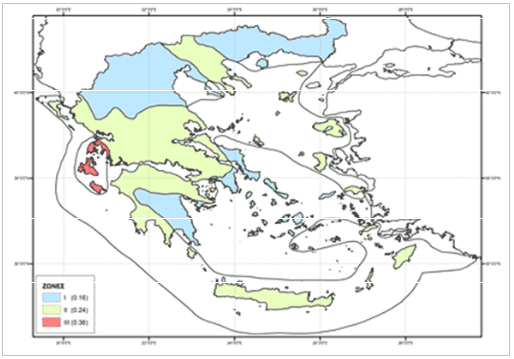
\includegraphics [scale = 0.80] {seismiki.png}
			\caption{Σεισμική επικινδυνότητα Ελλάδας}
			\label{seismiki}
		\end{center}
	\end{figure}
	
	Όπως είναι φανερό στο χάρτη σεισμικής επικινδυνότητας το μεγαλύτερο μέρος της Περιφέρειας Πελοποννήσου έχει μεσαία σεισμική επικινδυνότητα (συντελεστής 0,24) ενώ μόνο ένα μέρος των νομών Αρκαδίας, Λακωνίας βρίσκονται στη ζώνη χαμηλής σεισμικής επικινδυνότητας (συντελεστής 0,16).
	
	Επίσης ο παρακάτω χάρτης δείχνει την κατολισθητική επικινδυνότητα στον Ελλαδικό χώρο. Ο χάρτης οδηγεί στο συμπέρασμα πως το μεγαλύτερο κομμάτι της Περιφέρειας έχει μικρή έως μηδαμινή επικινδυνότητα με εξαίρεση ίσως το βορειοδυτικό άκρο του νομού Μεσσηνίας και το βορειοδυτικό άκρο του νομού Κορινθίας, όπου η επικινδυνότητα θα μπορούσε να χαρακτηριστεί υψηλή και μέτρια, αντίστοιχα.
	
	\begin{figure} [H]
		\begin{center}
			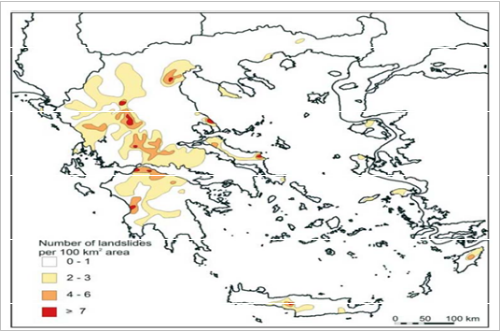
\includegraphics [scale = 0.80] {katolisthiseis.png}
			\caption{Κατολισθητική επικινδυνότητα Ελλάδας}
			\label{katolisthiseis}
		\end{center}
	\end{figure}
	
	\paragraph{Οικότοποι-Χλωρίδα-πανίδα}
	
	\textbf{Τύποι Οικοσυστημάτων}
	
	Στο έδαφος της Πελοποννήσου συνυπάρχουν διάφορα είδη οικοσυστημάτων. Σημαντικότερους από αυτούς είναι τα δάση, οι οικότοποι γλυκών υδάτων, οι βραχώδεις οικότοποι και τα σπήλαια καθώς και φυσικές και ημιφυσικές χλοώδεις διαπλάσεις και ρέοντα ύδατα.
	
	\textbf{Χλωρίδα-Πανίδα}
	
	Η Περιφέρεια Πελοποννήσου διαθέτει ποικιλία ειδών χλωρίδας και πανίδας,  τα οποία μπορεί να διαφοροποιούνται από νομό σε νομό και κυρίως με τις εναλλαγές τύπου οικοσυστήματος από χερσαίο σε υδάτινο και από ηπειρωτικό σε παραλιακό.
	
	\textbf{Ευαίσθητες και προστατευόμενες περιοχές}
	
	\underline{Δίκτυο NATURA 2000}
	
	\begin{figure} [H]
		\begin{center}
			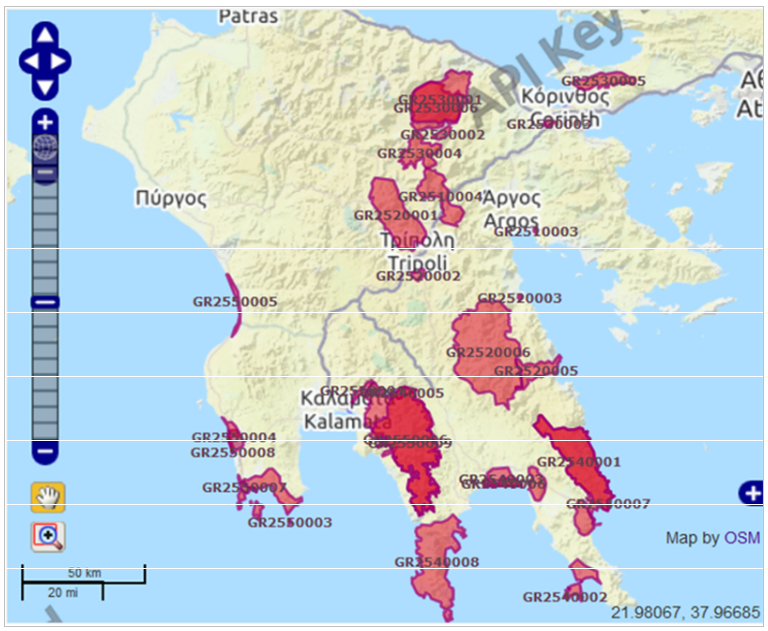
\includegraphics [scale = 0.60] {protected.png}
			\caption{Προστατευόμενες περιοχές NATURA 2000 Πελοποννήσου}
		\end{center}
	\end{figure}

	\begin{table}[H]
		\centering
		\label{my-label}
		\begin{tabular}{|l|}
			\hline
			\textbf{ΟΝΟΜΑ} \\
			\hline
			Ακροκόρινθος \\ \hline
			Ακροναυπλία και Παλαμήδι \\ \hline
			Εκβολές Ευρώτα \\ \hline
			Φαράγγι Νέδωνα (Πεταλόν-Χάνι) \\ \hline
			Κορυφές όρους Κυλλήνη (Ζήρεια) και χαράδρα Φλαμπουρίτσα \\ \hline
			Λαγκάδα Τρύπης \\ \hline
			Λίμνη Στυμφαλία \\ \hline
			Λίμνη Τάκα \\ \hline
			Λιμνοθάλασσα Γιάλοβας και Νήσος Σφακτηρία \\ \hline
			Λιμνοθάλασσα Μουστού \\ \hline
			Λιμνοθάλασσα Πύλου (Διβάρι) και Νήσος Σφακτηρία, Άγιος Δημήτριος \\ \hline
			Μονή Ελώνας και χαράδρα Λεωνιδίου \\ \hline
			Νήσοι Σαπιέντζα και Σχίζα, Ακρωτήριο Ακρίτας \\ \hline
			Νότια Μάνη  \\   \hline 
			Όρη ανατολικής Λακωνίας \\ \hline
			Όρη Αρτεμήσιο και Λύρκειο \\ \hline
			Όρη Γεράνεια \\ \hline
			Όρη Γιδοβούνι, Χιονοβούνι, Γαϊδουροβούνι, Κοράκια, Καλογεροβούνι,\\ Κουλοχέρα και περιοχή Μονεμβασιάς \\ \hline
			Όρος Μαίναλο \\ \hline
			Όρος Ολίγυρτος \\ \hline
			Όρος Πάρνωνας (και περιοχή Μαλεβής) \\ \hline
			Όρος Ταΰγετος  \\ \hline
			Όρος Ταΰγετος-Λαγκάδα Τρύπης \\ \hline
			Όρος Ζήρεια (Κυλλήνη) \\ \hline
			Περιοχή Νεάπολης και Νήσος Ελαφόνησος \\ \hline
			Θαλάσσια περιοχή Στενού Μεθώνης \\ \hline 
			Θίνες Κυπαρισσίας (Νεοχώρι-Κυπαρισσία) \\ \hline
			Υγρότοποι εκβολών Ευρώτα \\ 
			\hline
		\end{tabular}
	\caption{Προστατευόμενες περιοχές}
	\end{table}
	
	\underline{Καταφύγια Άγριας Ζωής}
	\begin{figure} [H]
		\begin{center}
			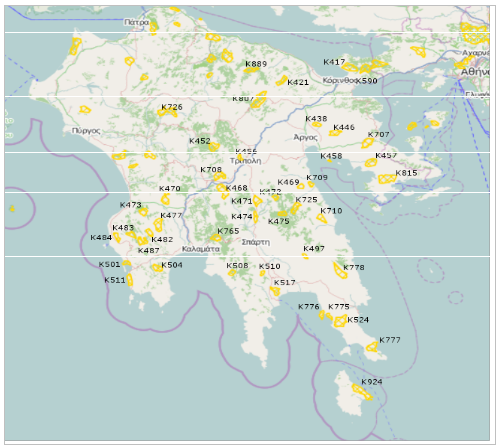
\includegraphics [scale = 0.90] {katafigia.png}
			\caption{Καταφύγια άγριας ζωής Πελοποννήσου}
		\end{center}
	\end{figure}

	\begin{table}[H]
		\centering
		
		\label{my-label}
		\begin{tabular}{ll}
			\hline
			\textbf{ΚΩΔΙΚΟΣ}         & \textbf{ΟΝΟΜΑ}          \\ \hline
			Κ889                     & Μπούτσι Ξυλοκάστρου  \\
			Κ421                     & Γκράβα-Λάκκα \\
			Κ807                     & Λίμνη Στυμφαλία \\
			Κ417                     & Γεράνεια (Λουτρακίου-Περαχώρας) \\
			Κ590                     & Πλάτανος (Λουτρακίου-Περαχώρας) \\
			Κ726                     & Λάδωνας \\
			Κ452					 & Αρκουδόρεμα-Χαλίκι \\
			Κ456					 & Δασώδης Περιοχή Αγ. Θεοδώρων \\
			Κ708 					 & Δάσος Παπαλέικο \\
			Κ468					 & Τσεμπερού \\
			Κ709					 & Υγροβιότοπος Μουστού \\
			Κ469					 & Μονή Παλαιοπαναγιάς \\
			Κ710					 & Κορομηλιά Λεωνιδίου \\
			Κ725					 & Φαράγγι Μαζιάς \\
			Κ472					 & Φονεμένοι Κυνουρίας \\
			Κ438					 & Πρ. Ηλίας-Δελόκορμο (Μυκήνες) \\
			Κ446					 & Μάλιζα-Τουρνέζα \\
			Κ458			 		& Νησίδες Ρόμβη-Δασκαλειό \\
			Κ707					& Κυνόρτιο  Όρος \\
			Κ457					& Σταυροπόδι-Καναρπίτσα \\
			Κ815					& Κάμπος Κρανιδίου \\
			Κ470					& Άνω Γλιάτα (Μάνδρας) \\
			Κ473					& Ροντάικα-Αγ. Νικόλαος\\
			Κ477					& Καλλιγάς (Τρικόρφου-Δραίνας) \\
			Κ482					& Τούμπα (Πλατανόβρυσης) \\
			Κ487					& Αμυγδαλίτσα \\
			Κ483 					& Ευρετή-Δενδρούλη-Αγ. Νικόλαος \\
			Κ484			  		& Σκοτωμένος Πετραλέξης (Γαργαλιάνων, Βάλτας, Φιλιατρών) \\
			Κ501					& Λίμνη Ντιβάρι \\
			Κ511					& Αγ. Νικόλαος \\
			Κ504					& Όρος Λυκόδημο \\
			Κ765					& Περιοχή Λαδά \\
			Κ508					& Ντουμπίτσια \\
			Κ471					& Κάμπος Καρυών \\
			Κ474					& Σελλασίας-Βρεσθένων \\
			Κ475					& Κουφοβούνι-Τσικούλιο \\
			Κ510					& Αναδασώσεις \\
			Κ517					& Λουτσάκα-Χαμοσπηλιά-Πέρα Βρύση \\
			Κ497					& Κάστρο Γερακίου \\
			Κ778					& Γαϊδουροβούνι \\
			Κ776					& Ξυλί Ασωπού \\
			Κ775					& Κάτω Κορογόνα \\
			Κ524					& Πράταγος-Αετοφωλιά \\
			Κ777					& Βαβίλα-Κούνος Νεαπόλεως \\
			Κ924					& Πρασονήσι Κυθήρων \\
			\hline                      
		\end{tabular}
		\caption{Καταφύγια Άγριας Ζωής}
	\end{table}

	\underline{Αισθητικά δάση}
	
	Το μοναδικό αισθητικό δάσος της Περιφέρειας Πελοποννήσου είναι το Δρυόδασος Μογγοστού Κορινθίας.
	
	\begin{figure} [H]
		\begin{center}
			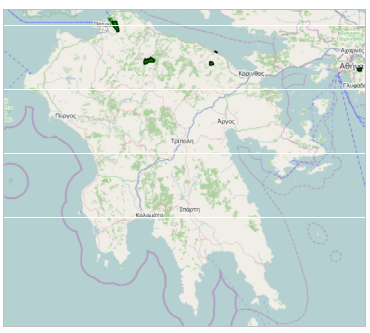
\includegraphics [scale = 0.90] {aisthitika.png}
			\caption{Αισθητικά δάση Πελοποννήσου}
		\end{center}
	\end{figure}
	
	\underline{Τοπία ιδιαίτερου φυσικού κάλους}
	
	\begin{figure} [H]
		\begin{center}
			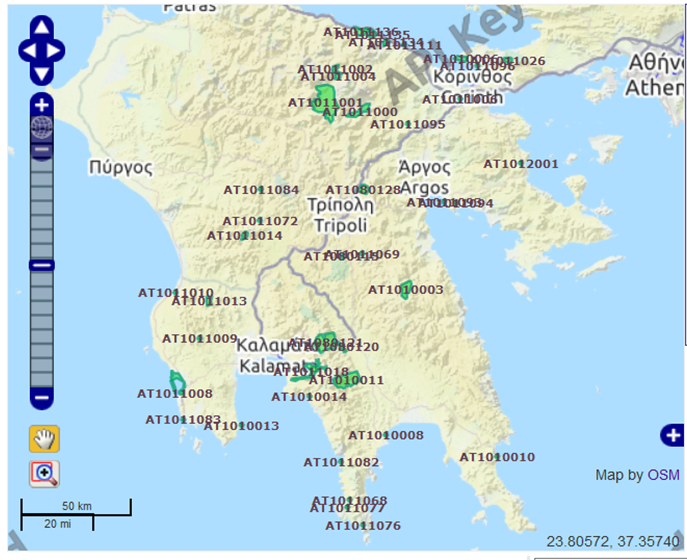
\includegraphics [scale = 0.60] {kallos.png}
			\caption{Τοπία ιδιαίτερου φυσικού κάλλους Πελοποννήσου}
		\end{center}
	\end{figure}

	\begin{table}[H]
		\centering
		\label{my-label}

		\begin{tabular}{|l|}
			\hline
			\textbf{ΟΝΟΜΑ} \\
			\hline
			Αισθητικό Δάσος Πευκιά Ξυλοκάστρου \\ \hline
			Ακροκόρινθος \\ \hline
			Ακροναυπλία και Παλαμήδι \\ \hline
			Ανώνυμος λόφος δυτικά της Ασίνης \\ \hline
			Άνω Πόλη Κυπαρισσίας \\ \hline
			Αρεόπολη \\ \hline
			Βάθεια \\ \hline
			Βουνό Παναγιάς Κορυφής \\ \hline
			Γύθειο \\ \hline
			Δημητσάνα, Στεμνίτσα και Φαράγγι Λουσίου \\ \hline
			Καρδαμύλη \\ \hline
			Καρύταινα \\ \hline
			Καστάνιτσα Πάρνωνα \\ \hline
			Κεντρικός Ταΰγετος  \\ \hline
			Κερασιά-Βλαχοκερασιά Αρκαδίας \\ \hline
			Κίττα \\ \hline
			Κοιλάδα Φενεού \\ \hline
			Κορώνη \\ \hline
			Λαγκάδα Ταϋγέτου \\ \hline
			Λίμνη Στυμφαλία \\ \hline
			Λόφος Παναγιά Νεμέας \\ \hline
			Λόφος Στόχος Νεστάνης (Τσιπιανών) \\ \hline
			Μανιάκι-Ταμπούρια Παπαφλέσσα \\ \hline
			Μεθώνη \\ \hline
			Μετέωρα Κορινθίας \\ \hline
			Μίνα Μάνης \\ \hline
			Μονεμβασιά \\ \hline
			Μονή Θεοτόκου Περχώρας \\ \hline
			Νέα Επίδαυρος \\ \hline
			Όρος Προφήτης Ηλίας (Λιούστρα) Μεσσηνίας \\ \hline
			Περιοχή Ηραίου Περαχώρας \\ \hline
			Περιοχή Μυστρά-Παρορίου-Αγίου Ιωάννου \\ \hline
		\end{tabular}
	\end{table}

	\begin{table}[H]
		\centering
		\label{my-label}
		
		\begin{tabular}{|l|}
			\hline
			Πέτρα Περαχώρας (Βράχος Βουνού) \\ \hline
			Πύλος και Όρμος Ναυαρίνου \\ \hline
			Υψώματα βόρεια του χωριού Στενό Κορινθίας \\ \hline
			Υψώματα Ελληνικού \\ \hline
			Υψώματα Λυγιάς \\ \hline
			Φαράγγι Κασκαράκας \\ \hline
			Φαράγγι ποταμού Νέδα \\ \hline
			Χώρος μάχης Βερβαίνων \\ \hline
			
		\end{tabular}
		\caption{Τοπία ιδιαίτερου φυσικού κάλλους Πελοποννήσου}
	\end{table}
	
	\underline{Βιότοποι Corine}
	
	\begin{figure} [H]
		\begin{center}
			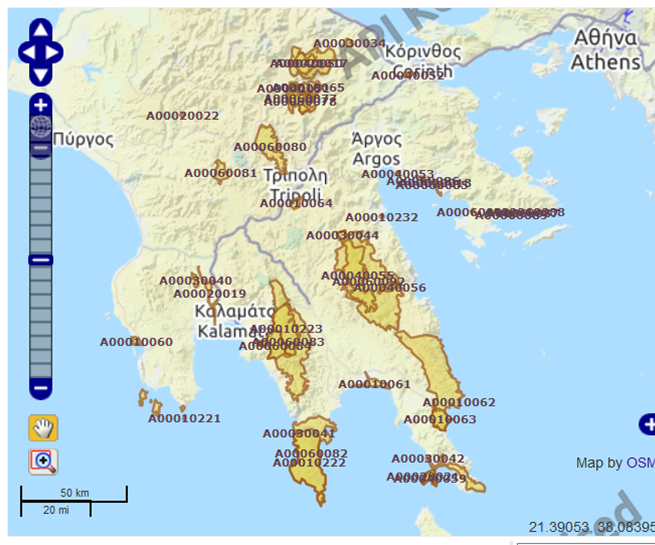
\includegraphics [scale = 0.60] {corine.png}
			\caption{Βιότοποι \selectlanguage{english}Corine \selectlanguage{greek}Πελοποννήσου}
		\end{center}
	\end{figure}

	\begin{table}[H]
		\centering
		\label{my-label}
		
		\begin{tabular}{|l|}
			\hline
			\textbf{ΟΝΟΜΑ} \\
			\hline
			Ακροκόρινθος \\ \hline
			Ακροναυπλία και Παλαμήδι \\ \hline
			Νήσοι Σαπιέντζα και Σχίζα, Ακρωτήριο Ακρίτας \\ \hline
			Βουνά Μονεμβασιάς \\ \hline
			Δάσος Μογκοστού, Βάλτου Σουλίου \\ \hline
			Διβάρι Πύλου \\ \hline
			Εκβολές Ευρώτα (Διβάρι και Λίμνη Αστερίου) \\ \hline
			Ελαφόνησος Λακωνίας \\ \hline
			Έλος χωριού Καντιά \\ \hline
			Κορυφές όρους Κυλλήνη (Ζήρεια) και χαράδρα Φλαμπουρίτσα \\ \hline
			Κορυφές Όρους Μαίναλο \\ \hline
			Κορυφές Όρους Ολίγυρτος \\ \hline
			Κορυφές Όρους Πάρνωνας \\ \hline
			Κορυφή Παρνιάς (Μαυροβούνι) \\ \hline
			Λίμνη Στρογγύλη (Βιγκλάφια) \\ \hline
			Λίμνη Στυμφαλία \\ \hline
			Λίμνη Τάκα \\ \hline
			Λιμνοθάλασσα Δρέπανου, Ναύπλιο \\ \hline
			Λιμνοθάλασσες Θερμισίας \\ \hline
			Μονή Ελώνας και χαράδρα Λεωνιδίου \\ \hline
			Μονή Μαλεβής \\ \hline
			Νότια Μάνη, Όρος Σαγγιάς και Ακρωτήριο Ταίναρο \\ \hline
			Όρη Γιδοβούνι, Χιονοβούνι, Γαϊδουροβούνι, Κοράκια, \\ Καλογεροβούνι, Κουλοχέρα  \\ \hline
			Όρος Ιθώμη \\ \hline
			Όρος Κεντρικός Ταΰγετος  \\ \hline
			Όρος Κυλλήνη (Ζήρεια) \\ \hline
			Όρος Ολίγυρτος \\ \hline
			Όρος Πάρνωνας \\ \hline
			Όρος Ταΰγετος  \\ \hline
			Περιοχή Νεάπολης Βιών και Νήσος Ελαφόνησος \\ \hline
			Ποταμός Λάδων \\ \hline
			Ποταμός Πάμισος \\ \hline
		\end{tabular}
	\end{table}

	\begin{table}[H]
		\centering
		\label{my-label}
		\begin{tabular}{|l|}
			\hline
			Σπηλιά Γλυφάδα και Αλεπότρυπα Πύργου Δυρού \\ \hline
			Σπηλιά Φραχτή Ερμιονίδας \\ \hline
			Υγρότοποι Ερμιονίδας \\ \hline
			Υγρότοποι κόλπου Τολού, Ναύπλιο \\ \hline
			Υγρότοπος Μετόχι Ερμιονίδας \\ \hline
			Υγρότοπος Μουστού/Άστρος \\ \hline 
			Φαράγγια Κοσκάρακας και Βιρού \\ \hline
			Φαράγγι Λούσιου \\ \hline
			Χερσόνησος Μάνης \\ \hline
		\end{tabular}
		\caption{Βιότοποι \selectlanguage{english}Corine \selectlanguage{greek}Πελοποννήσου}
	\end{table}

	\paragraph{Κλιματολογικά-Μετεωρολογικά στοιχεία}
	
	Το κλίμα της Πελοποννήσου διαφέρει ανάλογα με την περιοχή και το υψόμετρο της. Είναι ήπιο και ζεστό στα παράλια και ψυχρό (αλλά υγιεινό) στο εσωτερικό. Γενικά η Πελοπόννησος είναι προνομιούχος περιοχή, από άποψη κλίματος, γιατί διαθέτει το χαρακτηριστικό μεσογειακό τύπο. Η θερμοκρασία παρατηρείται μεγαλύτερη στις περιοχές των Πατρών, της Καλαμάτας, του Πύργου καθώς επίσης και στην περιοχή του Άργους κι ελαττώνεται κατά πολύ στα ορεινά, π.χ. στην περιοχή της Τρίπολης. Όπως φαίνεται και στον παρακάτω χάρτη η ανατολική και νότια Πελοπόννησος έχει εύκρατο μεσογειακό κλίμα, η κεντρική -κυρίως στο νομό Αρκαδίας-έχει ορεινό κλίμα και η δυτική Πελοπόννησος έχει μεσογειακό κλίμα.
	
	Το \emph{μέσο ετήσιο ύψος βροχής} της δυτικής Πελοποννήσου είναι πάνω από 800 χιλιοστά, στην κεντρική κυμαίνεται μεταξύ 500-800 χιλιοστά και στην ανατολική κάτω από 500 χιλιοστά.
	
	\begin{figure} [H]
		\begin{center}
			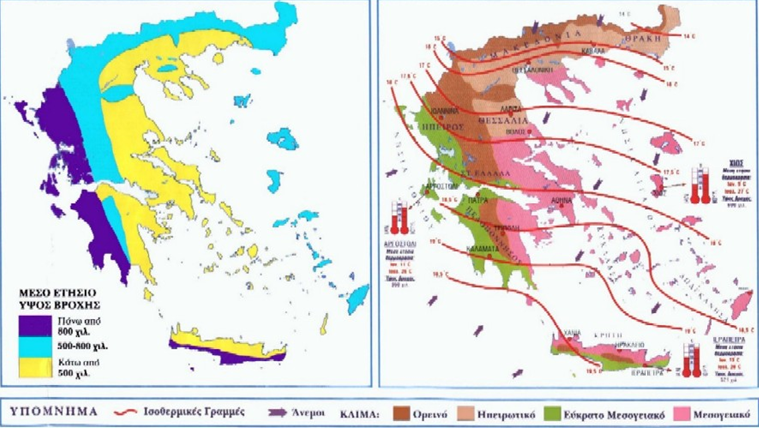
\includegraphics [scale = 0.60] {klima.png}
			\caption{Κλίμα Ελλάδας}
		\end{center}
	\end{figure}
	
	\subsubsection{Ανθρωπογενές Περιβάλλον}
	
	\paragraph{Πληθυσμιακά στοιχεία}
	
	Σύμφωνα με την απογραφή της ΕΛΣΤΑΤ του 2011, ο μόνιμος πληθυσμός της Περιφέρειας Πελοποννήσου ανέρχεται σήμερα σε 577.903 άτομα και κατανέμεται στους πέντε Νομούς που την απαρτίζουν ως ακολούθως: 
	
	\begin{itemize}
		\item 15\% στον Νομό Αρκαδίας 
		\item 17\% στον Νομό Αργολίδας 
		\item 25\% στον Νομό Κορινθίας 
		\item 15\% στον Νομό Λακωνίας 
		\item 28\% στον Νομό Μεσσηνίας
	\end{itemize}
	
	Η συγκέντρωση πληθυσμού στην Περιφέρεια έχει παραμείνει πρακτικά σταθερή την τελευταία δεκαετία (2001-2011), παρουσιάζοντας μια ελαφρά μείωση της τάξης του 3,0\%, ήτοι 0,3\% ετησίως.
	
	Αναλυτικά, η ποσοστιαία μείωση του πληθυσμού στη δεκαετία 2001-2011, ήταν 5\% (ήτοι 0,5\% ετησίως) για τους Νομούς Αρκαδίας και Αργολίδας, 4\% (ήτοι 0,4\% ετησίως) για τους Νομούς Λακωνίας και Μεσσηνίας, ενώ στο Ν. Κορινθίας ο πληθυσμός αυξήθηκε κατά 0,4\% (ήτοι 0,04\% ετησίως).
	
	\paragraph{Χρήσεις γης}
	
	\begin{figure} [H]
		\begin{center}
			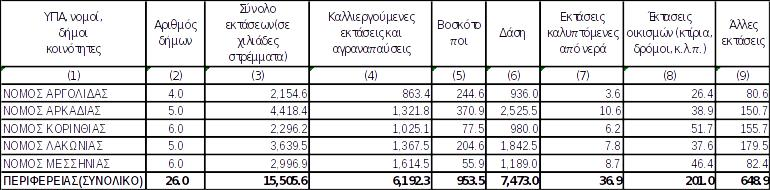
\includegraphics [scale = 0.80] {xriseis.jpg}
			\caption{Χρήσεις γης}
		\end{center}
	\end{figure}
	
	\paragraph{Κοινωνικό-Οικονομικό περιβάλλον}
	
	\textbf{Οικονομία-Γενικά στοιχεία}
	
	Ο συνολικά οικονομικά ενεργός πληθυσμός της περιφέρειας Πελοποννήσου (ΕΛΣΤΑΤ) παραμένει σχεδόν σταθερός διαχρονικά από το 2010 έως το 2014, δηλαδή από 253,2 χιλιάδες εργατικού δυναμικού το 2010, το 2014 το εργατικό δυναμικό είναι της τάξης των 246,2 χιλιάδων. Παρατηρείται ωστόσο μεγάλη μείωση του απασχολούμενου πληθυσμού από τις 228,8 χιλιάδες σε 188,7 χιλιάδες αριθμός των ανέργων ξεπερνάει το διπλάσιο του έτους 2010 ο οποίος ήταν 24,4 χιλιάδες και φτάνει το 2014 σε 57,5 χιλιάδες. Επομένως το ποσοστό ανεργίας αυξάνεται από το 9,6\% σε 23,4\% το 2014.
	
	\textbf{Πρωτογενής τομέας}
	
	Σε ότι αφορά την απασχόληση στο Πρωτογενή Τομέα, η Περιφέρεια Πελοποννήσου βρίσκεται στη πρώτη θέση ανάμεσα σε όλες τις Περιφέρειες της  χώρας, αναφορικά με το μερίδιο της απασχόλησης στο Πρωτογενή τομέα. Συγκεκριμένα, στη Περιφέρεια απορροφάται το 29,4\% του απασχολούμενου πληθυσμού, όταν ο Μ.Ο. της χώρας ανέρχεται μόλις στο 12,5\%.
	
	Στη Περιφέρεια Πελοποννήσου όσον αφορά στον \textbf{\underline{αγροτικό τομέα}} παράγεται σημαντικός αριθμός προϊόντων ΠΟΠ (Προστατευόμενης Ονομασίας Προέλευσης) και ΠΓΕ (Προστατευόμενης Γεωγραφικής Ένδειξης), όπως; Ελιές, Ελαιόλαδο, Τυριά, Φρούτα, Λαχανικά, Ξηροί Καρποί, Όσπρια και Προϊόντα Ζωικής Προέλευσης. Η σχετική θέση του πρωτογενή τομέα της Περιφέρειας Πελοποννήσου, σε σύγκριση και με το μέγεθος του τομέα στη χώρα είναι ιδιαίτερα σημαντική.
	
	Η \textbf{\underline{κτηνοτροφία}} διαδραματίζει δευτερεύοντα ρόλο στην Περιφέρεια. Ο σημαντικότερος κτηνοτροφικός κλάδος είναι τα γαλακτοκομικά και τα κυριότερα κτηνοτροφικά προϊόντα που παράγονται είναι το μέλι, τα ψάρια εσωτερικών υδάτων, τα αυγά, το μαλακό τυρί και τα μαλλιά προβάτων.
	
	\paragraph{Δευτερογενής τομέας}
	
	Στην Περιφέρεια ο δευτερογενής τομέας είναι ο ισχνότερος οικονομικός τομέας και παρουσιάζει μείωση του ποσοστού συμμετοχής του στο συνολικό Ακαθάριστο Προϊόν της Περιφέρειας, η οποία όμως είναι αντίστοιχη της κάμψης που παρατηρείται σε επίπεδο χώρας. Ο τομέας αυτός επηρεάζεται από τις βιομηχανικές ζώνες της Περιφέρειας Αττικής και από την παρουσία του δεύτερου σημαντικότερου ενεργειακού κέντρου της χώρας στη Μεγαλόπολη. Κυρίαρχη δραστηριότητα του δευτερογενή τομέα στην Περιφέρεια Πελοποννήσου είναι η Μεταποίηση, η οποία παράγει το 65\% της Ακαθάριστης Προστιθέμενης Αξίας του δευτερογενή τομέα. Δεύτερη σημαντική δραστηριότητα είναι οι κατασκευές, με συμμετοχή 20\% στην ΑΠΑ του δευτερογενούς τομέα, ενώ την τρίτη θέση καταλαμβάνουν οι δραστηριότητες του κλάδου ενέργειας. Οι κύριες ειδικεύσεις των ΠΕ της Περιφέρειας αφορούν κυρίως τους κλάδους Τροφίμων, Ξύλου, Ποτών και Μη Μεταλλικών Ορυκτών, δηλαδή κλάδοι που είτε αναφέρονται στην επεξεργασία προϊόντων του πρωτογενή τομέα, είτε στις κατασκευές. Στο επίπεδο Περιφερειακών Ενοτήτων, δεν εμφανίζονται σημαντικές διακυμάνσεις στην παραγόμενη Ακαθάριστη Προστιθέμενη Αξία. Οι ΠΕ Αρκαδίας και Μεσσηνίας, βελτιώνουν τη θέση τους, ενώ αντίθετα οι ΠΕ Αργολίδας και Λακωνίας διατηρούνται σταθερές.
	
	\paragraph{Τριτογενής τομέας}
	
	Ο τριτογενής τομέας στην Περιφέρεια Πελοποννήσου απορροφά το 52,1\% της απασχόλησης στη Περιφέρεια το 2010 (έναντι 67,8\% του τομέα στο σύνολο της χώρας), μια επίδοση που κατατάσσει τη Περιφέρεια στην ενδέκατη θέση μεταξύ των Περιφερειών της χώρας. Ειδικότερα, ο τριτογενής τομέας στην Περιφέρεια Πελοποννήσου απασχολεί το 40\% των εργαζομένων της Περιφέρειας, με σημαντικές ποσοτικές διαφοροποιήσεις ανά έτος στον αριθμό των απασχολούμενων, φαινόμενο που υποδεικνύει μια «ρευστότητα» στις οικονομικές δραστηριότητες του τριτογενή τομέα. Ο μεγάλος όγκος των επιχειρήσεων και λοιπών λειτουργιών του τριτογενή τομέα, όπως διοικητικές, εκπαιδευτικές, χρηματοπιστωτικές και εμπορικές υπηρεσίες, καθώς και οι υπηρεσίες των μεταφορών, είναι συγκεντρωμένες στα αστικά κέντρα της Περιφέρειας, ενώ οι τουριστικές υπηρεσίες που εκφράζονται κατά κύριο λόγο από τον κλάδο των «Ξενοδοχείων και εστιατορίων» παρουσιάζουν χωρική διασπορά στην Περιφέρεια. Ο τουρισμός θεωρείται κρίσιμος παράγοντας για την ανάπτυξη του τριτογενούς τομέα στην Περιφέρεια, αναπτύσσεται ωστόσο με αργούς ρυθμούς διατηρώντας ένα χαμηλό ποσοστό συμμετοχής στη συνολική τουριστική δραστηριότητα της χώρας. Σαφής είναι η τάση αύξησης των τουριστικών αφίξεων την περίοδο 2002-2010 στην Περιφέρεια Πελοποννήσου. Στην ευρύτερη περιοχή, διαχρονικά σημαντικοί τουριστικά προορισμοί αποτελούν οι ΠΕ Αργολίδας και Κορινθίας, οι οποίες διατηρούν ή/και αυξάνουν διαχρονικά το ειδικό τους βάρος στις αφίξεις τουριστών. Το μικρότερο μερίδιο στον τουριστικό κλάδο κατέχει η ΠΕ Αρκαδίας. Όσον αφορά στη ζήτηση τουριστικών υπηρεσιών (βάση των στοιχείων του 2010), η Περιφέρεια Πελοποννήσου αν και απορροφά το 6,6\% των συνολικών αφίξεων της χώρας, το μερίδιο της στις διανυκτερεύσεις ανέρχεται μόλις στο 3,8\%. Συνοπτικά συνάγεται ότι στην Περιφέρεια Πελοποννήσου ο τουρισμός είναι δραστηριότητα που βρίσκεται σήμερα σε χαμηλά επίπεδα, αλλά βαίνει διαχρονικά αυξανόμενη, στηριζόμενη σε συγκριτικά πλεονεκτήματα που παρουσιάζει η περιοχή.  
	
	\paragraph{Υφιστάμενες Τεχνικές υποδομές}
	
	\textbf{Δίκτυο μεταφορών}
	
	\begin{enumerate}
		\item \textbf{Οδικό δίκτυο} \\
		Το οδικό δίκτυο της Περιφέρειας είναι ιδιαίτερα εκτεταμένο, λόγω της έκτασης και της γεωμορφολογίας του εδάφους. Το εθνικό δίκτυο εκτείνεται σε 1.250 χλμ. περίπου, ενώ το επαρχιακό οδικό δίκτυο εκτείνεται σε μήκος 4.600 χλμ. περίπου. Στα παράλια και στα πεδινά είναι περισσότερο ανεπτυγμένο, ενώ είναι σχετικά ανεπαρκές, ποσοτικά και ποιοτικά, στις ορεινές περιοχές. Ο κυριότερος οδικός άξονας που διαπερνά την Περιφέρεια Πελοποννήσου ενώνοντας τα κυριότερα αστικά κέντρα μεταξύ τους είναι ο αυτοκινητόδρομος, ο οποίος συνδέει την Καλαμάτα με την Τρίπολη και την Κόρινθο και κατ’ επέκταση με την Αθήνα. Επιπρόσθετα, σημαντικός αναπτυξιακός παράγοντας για την Περιφέρεια είναι η διέλευση από το βόρειο τμήμα της, μεγάλου μέρους του οδικού άξονα ΠΑΘΕ. Τέλος, στην Περιφέρεια Πελοποννήσου προβλέπεται να καταλήξει η Ολυμπία Οδός.
		
		Οι κυριότεροι οδοί που απαρτίζουν το οδικό δίκτυο της Περιφέρειας παρουσιάζονται συνοπτικά ακολούθως:
		
		\textbf{Αυτοκινητόδρομοι}
		\begin{itemize}
			\item Α7. Κόρινθος  – Τρίπολη  – Μεγαλόπολη  – Καλαμάτα (του Ε65)
			\item Α8. Ελευσίνα – Μέγαρα  – Κόρινθος  –Αίγιο  – Ρίο (Τμήμα των Ε94 \& Ε65)
			\item Πύργος  – Καλό Νερό  – Αλλαγή  – Καλαμάτα (9α) (Τμήμα του Ε55)
			\item Α71. Λεύκτρο (Μεγαλόπολη  – Σπάρτη (Τμήμα του Ε961  – Υπό κατασκευή)
		\end{itemize}
		\textbf{Εθνικό Οδικό Δίκτυο}
		\begin{itemize}
			\item 8α. Ελευσίνα - Μέγαρα  -Κινέτα - Άγιοι Θεόδωροι - Λουτράκι - Κόρινθος - Κιάτο - Ξυλόκαστρο - Δερβένι  - Ακράτα - Διακοπτό - Αίγιο - Λόγγος - Ρίο - Πάτρα
			\item 10. Ίσθμια - Αλμύρι - Νέα Επίδαυρος - Παλαιά Επίδαυρος - Λυγούριο
			\item 66. Εθνική Οδός 7στο σιδηροδρομικό σταθμό Νεμέας) - Νεμέα - Ψάρι - Σκοτεινή - Κανδήλα - Λεβίδι
			\item 70. Άργος - Ναύπλιο - Θέατρο Επιδαύρου - Παλαιά Επίδαυρος 
			\item 82. Σπάρτη - Καλαμάτα - Μεσσήνη - Βελίκα - Χατζή - Πύλος
			\item 76. Μεγαλόπολη - Ανδρίτσαινα - Ναός Επικουρείου Απόλλωνος
			\item 74. Τρίπολη - Λεβίδι - Βυτίνα - Ολυμπία - Βαρβάσαινα - Πύργος
			\item 39.Τρίπολη - Σπάρτη - Γύθειο
			\item 9. Πάτρα - Πύργος - Κυπαρισσία - Πύλου - Μεθώνη
		\end{itemize}
		\begin{figure} [H]
			\begin{center}
				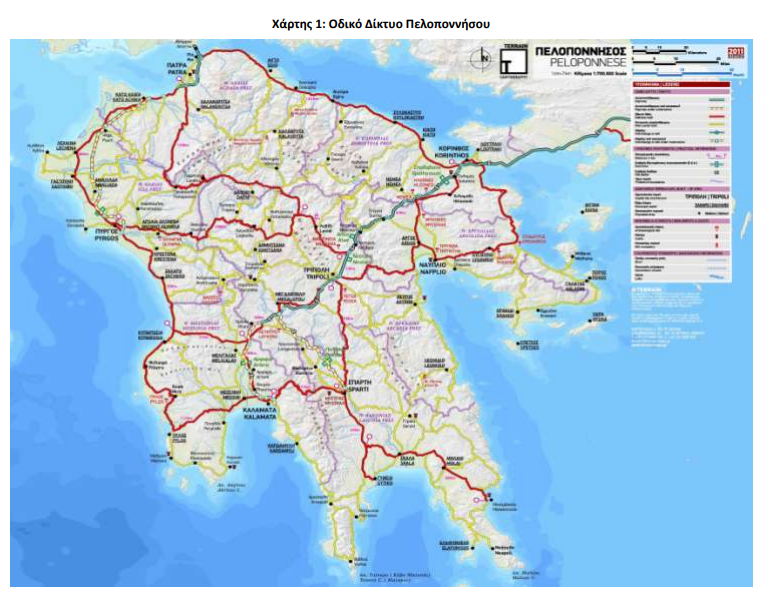
\includegraphics [scale = 0.60] {peloponnisos2.png}
				\caption{Οδικός χάρτης Πελοποννήσου}
			\end{center}
		\end{figure}
		\item \textbf{Σιδηροδρομικό δίκτυο} \\
		Σημαντικό ρόλο στην ανάπτυξη του βόρειου μέρους της Περιφέρειας Πελοποννήσου, έχει διαδραματίσει η λειτουργία του Προαστιακού Σιδηρόδρομου που συνδέει την Αττική με το Κιάτο. Διεξάγονται καθημερινά 6 δρομολόγια με συχνότητα δύο ωρών. Η απόσταση Αθήνα -Κιάτο διαρκεί 1 ώρα και 17 λεπτά. Ο Προαστιακός έχει συμβάλει αποφασιστικά στην ασφαλή διακίνηση εργαζομένων, επισκεπτών από και προς την Πρωτεύουσα της χώρας, στην προσέλκυση πληθυσμού για παραθεριστική κατοικία και συνολικά στη συγκράτηση του πληθυσμού της ΠΕ Κορινθίας. Αντίθετα το υπόλοιπο σιδηροδρομικό δίκτυο στην Πελοπόννησο έχει εγκαταλειφθεί με ελάχιστες εξαιρέσεις στον βόρειο άξονα. Παλαιότερα υπήρχε τρένο που σύνδεε την Αθήνα με την Καλαμάτα, μέσω Τρίπολης, αλλά από το 2010 η γραμμή έχει διακοπεί (όπως και οι γραμμές Πύργος –Καλαμάτα, Καλαμάτα -Μεσσήνη –ΤΕΙ και Κόρινθος -Τρίπολη –Ναύπλιο). Το σιδηροδρομικό δίκτυο στην Περιφέρεια Πελοποννήσου, έχει συνολικό μήκος 300 χλμ., όμως οι περισσότερες  γραμμές του δικτύου του είναι μονής κατεύθυνσης, δεν υπάρχουν ανισόπεδες διαβάσεις και υπήρχε κακή χάραξη.
		
		Συμπερασματικά για το σιδηροδρομικό δίκτυο στην Περιφέρεια Πελοποννήσου, θα πρέπει να εκπονηθούν μελέτες βιωσιμότητας για να εξετασθούν η επαναφορά του ενδομεσσηνιακού δικτύου, η ενεργοποίηση των ιστορικών γραμμών Κόρινθος –Μυκήνες –Άργος –Ναύπλιο, καθώς και της προέκτασης του προαστιακού προς το Λουτράκι, προκειμένου να ερευνηθούν βάσει μελέτης κόστους-οφέλους αν υφίστανται οι προϋποθέσεις πλήρους επαναλειτουργίας του, ή αν χρησιμοποιηθεί μόνο για αναβίωση και ανάδειξη πολιτιστικών διαδρομών.
		
		\item \textbf{Αεροδρόμια} \\
		Η Περιφέρεια Πελοποννήσου διαθέτει δύο αεροδρόμια. Ένα στρατιωτικό με έδρα την Τρίπολη και ένα πολιτικό με έδρα την Καλαμάτα, τον κρατικό αερολιμένα «Καπετάν Βασίλης Κωνσταντακόπουλος». Οι πολύ μικρής κλίμακας αεροπορικές συγκοινωνίες εξυπηρετούνται από το αεροδρόμιο της Καλαμάτας, με ενεργή μόνο την εβδομαδιαία σύνδεση με τη Θεσσαλονίκη. Η λειτουργία του αεροδρομίου της Καλαμάτας αυξάνεται κατά τους θερινούς μήνες από πτήσεις charter εξωτερικού. Στις δυσλειτουργίες του αεροδρομίου εντάσσεται η χρησιμοποίηση των αεροδιαδρόμων της από τις εκπαιδευτικές πτήσεις στρατιωτικών σκαφών της γειτνιάζουσας σε αυτό πολεμικής βάσης της αεροπορίας. Το τελευταίο διάστημα καταβάλλονται προσπάθειες από τοπικούς φορείς για τη μετατροπή του στρατιωτικού αεροδρομίου της Τρίπολης σε πολιτικό, για την εξυπηρέτηση πτήσεων χαμηλού κόστους, καθώς και για τον εκσυγχρονισμό του αεροδρομίου της Καλαμάτας. Απώτερο στόχο αποτελεί η βελτίωση της εξωστρέφειας της Περιφέρειας με την προσέλκυση αλλοδαπών τουριστών και η δημιουργία προϋποθέσεων ανάδειξής της ως ένα από τους κυριότερους αναγνωρίσιμους τουριστικούς προορισμούς, αξιοποιώντας το γεωγραφικό ανάγλυφο της και συνδυάζοντας τις διακοπές βουνό και θάλασσα.
		\item \textbf{Λιμένες} \\
		Στις θαλάσσιες μεταφορές, σημαντικό ρόλο παίζουν τα λιμάνια της Καλαμάτας και του Ναυπλίου. Άλλα δευτερεύοντα λιμάνια της Περιφέρειας είναι της Πύλου και της Κυπαρισσίας στη Μεσσηνία, της Ερμιονίδας και του Πορτοχελίου στην Αργολίδα, του Παράλιου Άστρους και του Λεωνιδίου στην Αρκαδία, της Κορίνθου και του Κιάτου στην Κορινθία και τέλος, του Γυθείου και της Νεάπολης στην Λακωνία. Τους θερινούς μήνες εκτελείται ένα δρομολόγιο την εβδομάδα που συνδέει τα Χανιά (Κίσσαμος) με τα Κύθηρα και την Καλαμάτα. Επίσης τους θερινούς μήνες εκτελούνται τακτικά δρομολόγια από Γύθειο για Κύθηρα και υπάρχει σύνδεση από Νεάπολη Λακωνίας για Κύθηρα και Ελαφόνησο. Επίσης, υπάρχει σύνδεση όλο τον χρόνο με θαλάσσιο ταξί από την Κόστα Αργολίδας με τις Σπέτσες και την Ύδρα. Τέλος, υπάρχει σύνδεση με ferry boat μεταξύ Γαλατά (Αργολίδας) και Πόρου. Τα περισσότερα λιμάνια-μαρίνες-αγκυροβόλια τα διαθέτει η ΠΕ Λακωνίας και η ΠΕ Κορινθίας. Ειδικότερα, η ΠΕ Λακωνίας έχει 22, η ΠΕ Κορινθίας έχει 14, η ΠΕ Αρκαδίας έχει 3 και οι ΠΕ Αργολίδας και Μεσσηνίας από δύο. Ο συνολικός κατάλογος των λιμενικών υποδομών του Νομού Μεσσηνίας (λιμάνια, μαρίνες και αγκυροβόλια είναι στην Καλαμάτα και στην Πύλο. Οι τρεις σημαντικότερες μαρίνες είναι της Καλαμάτας που έχει χωρητικότητα 300 θέσεων, του Ξυλόκαστρου με 220 θέσεις και η μαρίνα της Πύλου που κατασκευάστηκε πρόσφατα και διαθέτει 250 θέσεις.
	\end{enumerate}

	\textbf{Δίκτυα οργανισμών κοινής ωφέλειας}
	
	\begin{enumerate}
		\item \textbf{Δίκτυα ύδρευσης-άρδευσης} \\
		Τα ποιοτικά χαρακτηριστικά του νερού προς ύδρευση βρίσκονται υπό τον έλεγχο του Κράτους ή της Τοπικής Αυτοδιοίκησης. Αρμόδιο Υπουργείο για την ύδρευση είναι το Εσωτερικών, Δημόσιας Διοίκησης και Αποκέντρωσης και τοπικά οι σύνδεσμοι δήμων και κοινοτήτων, οι Δημοτικές επιχειρήσεις Ύδρευσης και Αποχέτευσης (ΝΠΙΔ) και οι Οργανισμοί Τοπικής Αυτοδιοίκησης. Σε τοπικό επίπεδο οι υδρευτικές ανάγκες κοινοτήτων και μικρών δήμων εξυπηρετούνται από μικρά υδρευτικά έργα που τα διαχειρίζονται οι ίδιοι οι ΟΤΑ. Τα κυριότερα προβλήματα των υπαρχόντων δικτύων, αφορούν την συντήρηση και τον εμπλουτισμό τους, καθώς και την αντικατάσταση των παλαιών δικτύων που έχουν κατασκευασθεί από τσιμεντοσωλήνες και παρουσιάζουν διαρροές από διάρρηξη ή εμφράξεις από τη συσσώρευση αλάτων.
		
		Στην Περιφέρεια Πελοποννήσου λειτουργούν 68 συλλογικά οργανωμένα \textbf{αρδευτικά δίκτυα}, με συνολική αρδεύσιμη έκταση περίπου 295.000 στρεμμάτων και ανάγκες  περίπου 101.156.000 \selectlanguage{english}$m^3$/\selectlanguage{greek}έτος. Οι διαχειριστές και πάροχοι των οργανωμένων αρδευτικών δικτύων είναι οι Τοπικοί Οργανισμοί Εγγείων Βελτιώσεων (ΤΟΕΒ), ο Γενικός Οργανισμός Εγγείων Βελτιώσεων (ΓΟΕΒ), καθώς και Δημοτικές Ενότητες. Τα νερά που χρησιμοποιούνται για άρδευση προέρχονται τόσο από γεωτρήσεις, όσο και από επιφανειακά απολήψεις. Τα κυριότερα συστήματα άρδευσης που χρησιμοποιούνται είναι κυρίως η στάγδην άρδευση, η επιφανειακή άρδευση και η τεχνητή βροχή. Οι ιδιωτικές γεωτρήσεις που υπάρχουν και λειτουργούν στην Περιφέρεια αρδεύουν περίπου 422.833.000 \selectlanguage{english}$m^3$/\selectlanguage{greek}έτος (σχεδόν το τετραπλάσιο των οργανωμένων αρδευτικών δικτύων). Οι πολυάριθμες ιδιωτικές γεωτρήσεις που λειτουργούν στην Περιφέρεια σε συνδυασμό με τις αυξημένες ανάγκες για άρδευση (δεδομένου των γεωργικών εκτάσεων που υπάρχουν στην Περιφέρεια) και την υπερεκμετάλλευση του εδάφους για γεωργικές καλλιέργειες, δημιουργούν προβλήματα μειωμένης ποσότητας νερού για άρδευση καθώς και αυξημένα προβλήματα μόλυνσης και υφαλμύρινσης του υδροφόρου ορίζοντα.
		
		Άλλοι σημαντικοί χρήστες νερού στην Περιφέρεια Πελοποννήσου είναι η βιομηχανική και η κτηνοτροφική δραστηριότητα. Οι ανάγκες των βιομηχανιών σε νερό που εδρεύουν στην Περιφέρεια Πελοποννήσου, ανέρχονται σε περίπου 20.877.000 \selectlanguage{english}$m^3$/\selectlanguage{greek}έτος και καλύπτονται από ιδιωτικές γεωτρήσεις ή από τροφοδοσία των δικτύων ύδρευσης. Οι κτηνοτροφικές και πτηνοτροφικές δραστηριότητες, τόσο σε μονάδες σταβλισμένων ζώων όσο και σε ζώα με ποιμενική εκτροφή, δημιουργούν ανάγκες σε νερό που φτάνουν περίπου τα 21.000.000 \selectlanguage{english}$m^3$/\selectlanguage{greek}έτος. Η κάλυψη των αναγκών νερού στη σταβλισμένη κτηνοτροφία προέρχεται από ιδιωτικές γεωτρήσεις ή από τροφοδοσία των δικτύων ύδρευσης ενώ οι ανάγκες της ποιμενικής κτηνοτροφίας καλύπτονται σε ένα ποσοστό τους και από επιφανειακά νερά.
		
		\item \textbf{Ενεργειακή υποδομή} \\
		Η περιοχή της Πελοποννήσου (μαζί με την περιοχή της Αττικής) αποτελούν τις πιο κρίσιμες περιοχές του νοτίου συστήματος παραγωγής ηλεκτρικής ενέργειας της χώρας δεδομένου ότι αποτελούν τις κυριότερες εγκαταστάσεις που βρίσκονται στο νότιο μέρος της Ελλάδος και λειτουργούν επικουρικά για την εξυπηρέτηση της Αθήνας. Στην Περιφέρεια Πελοποννήσου παράγεται περίπου το 8\% της συνολικής ηλεκτρικής ενέργειας της Δ.Ε.Η. πανελλαδικά με τη συμβολή των θερμοηλεκτρικών και υδροηλεκτρικών σταθμών στη Μεγαλόπολη και τον Λάδωνα αντίστοιχα, ενώ στις εγκαταστάσεις των σταθμών παραγωγής απασχολείται σημαντικός αριθμός εργαζομένων (2.628 εργαζόμενοι το τέλος του 2010). Προβλήματα επάρκειας ηλεκτρικής ενέργειας δεν παρουσιάζονται (κατά το μεγαλύτερο μέρος του έτους η περιοχή χαρακτηρίζεται εξαγωγική), παρά μόνο κατά τους θερινούς μήνες οπότε εισάγεται ρεύμα από σταθμούς εκτός Πελοποννήσου. Με πόρους που προέρχονται από το Τέλος Ανάπτυξης Βιομηχανικών Περιοχών παραγωγής ηλεκτρικού ρεύματος από Λιγνιτικούς Σταθμούς (γνωστό ως "λιγνιτόσημο", που ανέρχεται στο 0,4\% του Ετήσιου Κύκλου Εργασιών της Δ.Ε.Η. Α.Ε.), χρηματοδοτούνται τα πενταετή Ειδικά Αναπτυξιακά Προγράμματα, που περιλαμβάνουν έργα υποδομής, προστασίας του περιβάλλοντος και τόνωσης της οικονομίας της περιοχής της Μεγαλόπολης.
		
		\underline{Φυσικό αέριο}
		
		Το Εθνικό Σύστημα Μεταφοράς Φυσικού Αερίου (ΕΣΜΦΑ) που αποτελεί ένα από τα σπουδαιότερα έργα υποδομής της σύγχρονης Ελλάδας, που υλοποιείται από τον Διαχειριστή του Εθνικού Συστήματος Φυσικού Αερίου, προβλέπει την κατασκευή αγωγού υψηλής πίεσης, μήκους 159 χλμ., που θα συνδέει το ΕΣΜΦΑ από το σταθμό στους Αγίους Θεοδώρους του Ν. Κορινθίας μέχρι τον Σταθμό Ηλεκτροπαραγωγής της ΔΕΗ στη Μεγαλόπολη, ενώ θα διέρχεται από την ευρύτερη περιοχή των πόλεων της Κορίνθου, του Άργους, του Ναυπλίου, της Τρίπολης και της Μεγαλόπολης. Το έργο εξασφαλίζει εκτός από την ομαλή και φιλική προς το περιβάλλον λειτουργία του Σταθμού Ηλεκτροπαραγωγής της ΔΕΗ στη Μεγαλόπολη, τις προϋποθέσεις για την τροφοδότηση με φυσικό αέριο βιομηχανικών, οικιακών και άλλων καταναλωτών της ευρύτερης περιοχής από την οποία διέρχεται. Το έργο έχει σχεδιασθεί με τρόπο ώστε να είναι εφικτή η μελλοντική επέκταση του δικτύου αγωγών σε Καλαμάτα και Σπάρτη, με στόχο το χερσαίο Σύστημα Υψηλής Πίεσης να καλύψει γεωγραφικά το σύνολο της Περιφέρειας Πελοποννήσου.
		
		\item \textbf{Υποδομές τηλεπικοινωνίας} \\
		Από άποψη τηλεπικοινωνιακών υποδομών, στην Περιφέρεια Πελοποννήσου έχει αναπτυχθεί στο σύνολο του, το Βασικό Σχέδιο Τηλεφωνίας του ΟΤΕ που προέβλεπε την εγκατάσταση ψηφιακών κέντρων σε όλες τις Περιφερειακές Ενότητες, ενώ περιλήφθηκε στο Δίκτυο «Σύζευξις» (Νησίδα 6), όπου εντάχθηκαν πλήθος δημόσιων υπηρεσιών που μείωσαν σημαντικά το κόστος επικοινωνίας (μεταξύ αυτών και αρκετών Διευθύνσεων της Περιφέρειας). Παράλληλα, τα τελευταία χρόνια στο πλαίσιο υλοποίησης του Επιχειρησιακού Προγράμματος «Κοινωνία της Πληροφορίας» του Γ' ΚΠΣ, στην Περιφέρεια αναπτύχθηκαν έργα ευρυζωνικότητας (χωρίς ιδιαίτερη ακόμη αξιοποίηση) που αυξάνουν την αποδοτικότητα, συμβάλλουν στην συνεχή κατάρτιση και τη δια βίου μάθηση των πολιτών, ενώ συνεισφέρουν στην ενίσχυση της ανταγωνιστικότητας των τοπικών επιχειρήσεων.
		
		\item \textbf{Λοιπές υποδομές} \\
		Η γενική επίδοση της Περιφέρειας Πελοποννήσου στον τομέα της καινοτομίας είναι πολύ χαμηλή. Βρίσκεται στο 56\% του μέσου όρου της Ελλάδας. Η επίδοση αυτή φαίνεται ακόμη πιο χαμηλή αν λάβουμε υπόψη ότι η γενική επίδοση της Ελλάδας βρίσκεται στο 40\% του μέσου όρου της Ε.Ε., καταλαμβάνοντας την τελευταία θέση. Αυτό σε μεγάλο βαθμό οφείλεται στον παραδοσιακό χαρακτήρα των επιχειρήσεων της Περιφέρειας. Συνολικά στην Περιφέρεια Πελοποννήσου λειτουργούν 909 επιχειρήσεις με απασχόληση μεγαλύτερη των 5 ατόμων. Οι πιο σημαντικές παραγωγικές δραστηριότητες στην Πελοπόννησο ανήκουν σε τρία μεγάλα παραγωγικά συμπλέγματα, εντός των οποίων οι επιχειρήσεις αναπτύσσουν σχέσεις συνεργασίας και περιφερειακές εφοδιαστικές αλυσίδες: α) στο αγροτο-βιομηχανικό σύμπλεγμα, β) στο τουριστικό σύμπλεγμα και γ) στο κατασκευαστικό σύμπλεγμα. Αναφορικά με τις κοινωνικές υποδομές στον τομέα της υγείας, υπηρεσίες παρέχονται από τις υπάρχουσες υποδομές 16 θεραπευτηρίων και τριάντα ενός Κέντρων Υγείας, με τα Περιφερειακά τους ιατρεία. Στην Τρίπολη λειτουργεί το Περιφερειακό Νοσοκομείο Πελοποννήσου, ενώ σε όλες τις πόλεις- πρωτεύουσες των νομών, αλλά και σε ημιαστικά κέντρα της Περιφέρειας, λειτουργούν νοσοκομειακές μονάδες, οι οποίες είτε είναι νεόδμητες, ή έχουν πρόσφατα βελτιώσει την κτιριακή υποδομή και τον εξοπλισμό τους. Οι συνολικές κλίνες θεραπευτηρίων στην Περιφέρεια φθάνουν τις 1.86 (2003), από τις οποίες οι 1.734 είναι δημόσιες, σε εννέα δημόσια νοσοκομεία και επτά ιδιωτικά θεραπευτήρια. Η εξυπηρέτηση του αστικού πληθυσμού της Περιφέρειας καλύπτεται από τις νοσοκομειακές μονάδες, ενώ ο πληθυσμός της υπαίθρου εξυπηρετείται από τα Κέντρα Υγείας και τα περιφερειακά ιατρεία. Η δευτεροβάθμια περίθαλψη καλύπτεται από τις είκοσι μία νοσοκομειακές μονάδες της Περιφέρειας. Υποδομές τριτοβάθμιας περίθαλψης δεν υπάρχουν στην Περιφέρεια Πελοποννήσου. Το επίπεδο παροχής υπηρεσιών περίθαλψης / υγείας σε γενικές γραμμές παρουσιάζει ελλείψεις, κυρίως στην ύπαιθρο / αγροτικές περιοχές λόγω, χωροθέτησης των Κέντρων Υγείας σε σχέση με τη διάρθρωση των ΟΤΑ, σε συνδυασμό με τις ελλείψεις σε ιατρικό και νοσηλευτικό προσωπικό, ενώ και στις νοσοκομειακές μονάδες της Περιφέρειας παρατηρούνται ελλείψεις σε αριθμό ιατρικών ειδικοτήτων. Σε ότι αφορά την τριτοβάθμια εκπαίδευση, στην περιφέρεια από το 2003 λειτουργεί το Πανεπιστήμιο Πελοποννήσου, με έδρα την Τρίπολη, του οποίου οι υποδομές και η οργανωτική του δομή αναπτύσσονται σταδιακά σε διάφορες πόλεις της Περιφέρειας (πρωτεύουσες νομών). Μέχρι σήμερα λειτουργούν έξι σχολές με εννέα τμήματα.
	\end{enumerate}

	\paragraph{Πολιτιστική Κληρονομιά}
	
	\underline{Νομός Κορινθίας}
	
	\begin{figure} [H]
		\begin{center}
			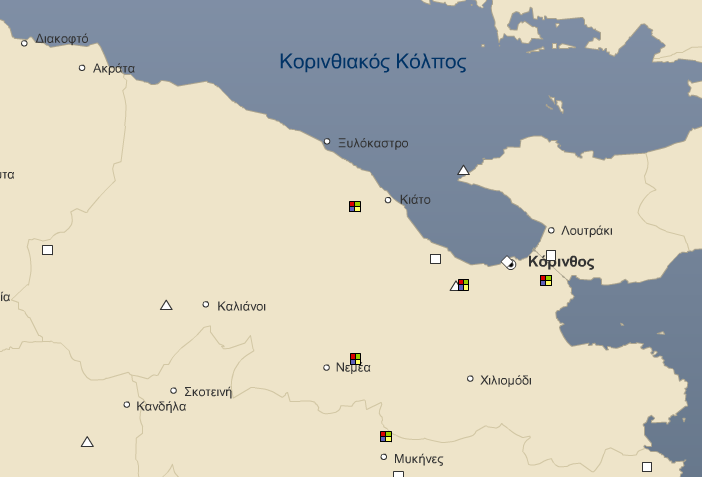
\includegraphics [scale = 0.60] {korinthia2.png}
			\caption{Πολιτιστική κληρονομιά Κορινθίας}
		\end{center}
	\end{figure}

	\underline{Νομός Αργολίδας}
	
	\begin{figure} [H]
		\begin{center}
			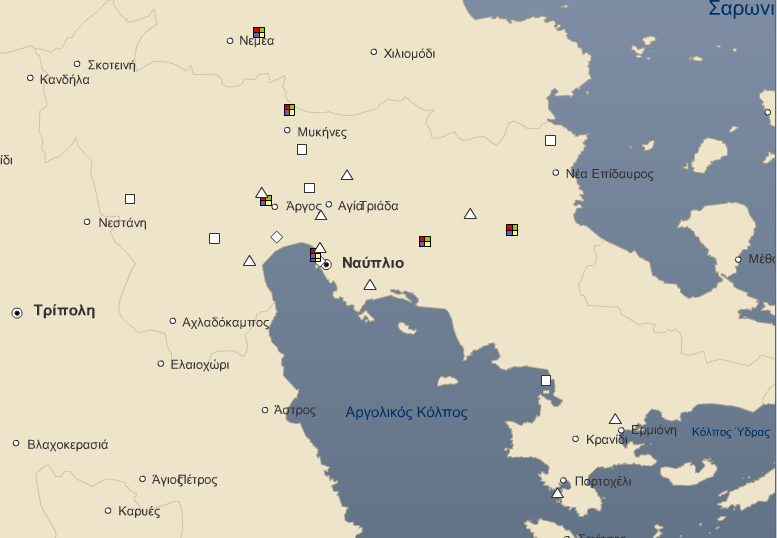
\includegraphics [scale = 0.60] {argolida2.png}
			\caption{Πολιτιστική κληρονομιά Αργολίδας}
		\end{center}
	\end{figure}
	
	\underline{Νομός Αρκαδίας}
	
	\begin{figure} [H]
		\begin{center}
			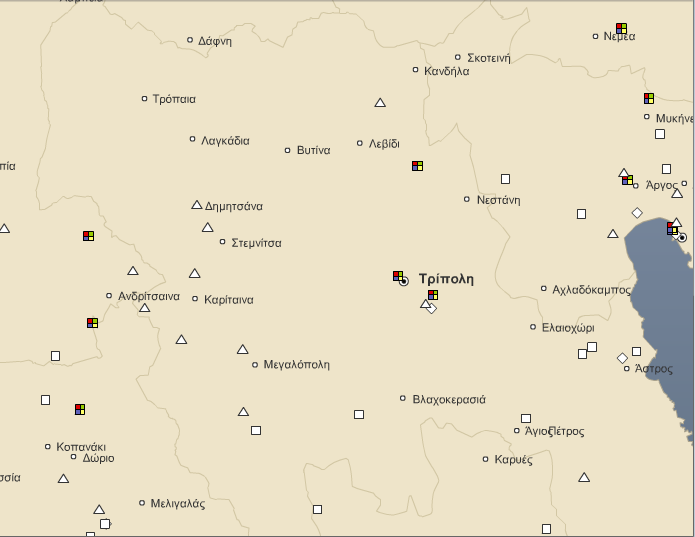
\includegraphics [scale = 0.60] {arkadia2.png}
			\caption{Πολιτιστική κληρονομιά Αρκαδίας}
		\end{center}
	\end{figure}

	\underline{Νομός Λακωνίας}
	
	\begin{figure} [H]
		\begin{center}
			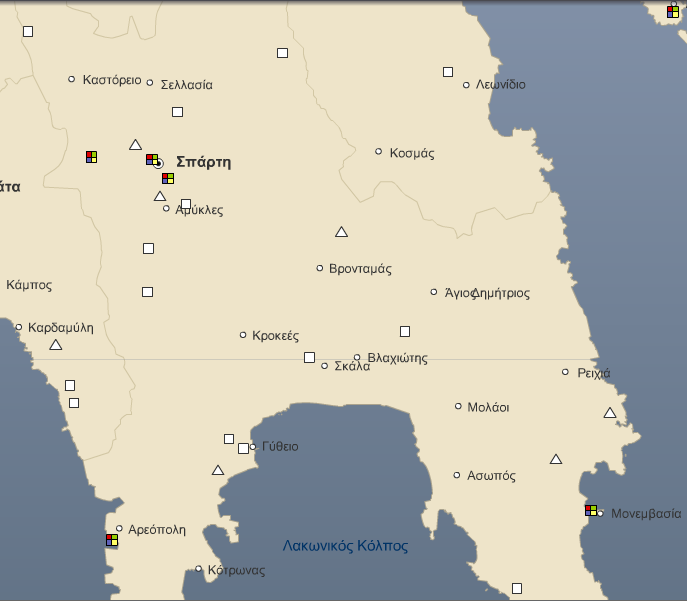
\includegraphics [scale = 0.60] {lakonia2.png}
			\caption{Πολιτιστική κληρονομιά Λακωνίας}
		\end{center}
	\end{figure}

	\underline{Νομός Μεσσηνίας}
	
	\begin{figure} [H]
		\begin{center}
			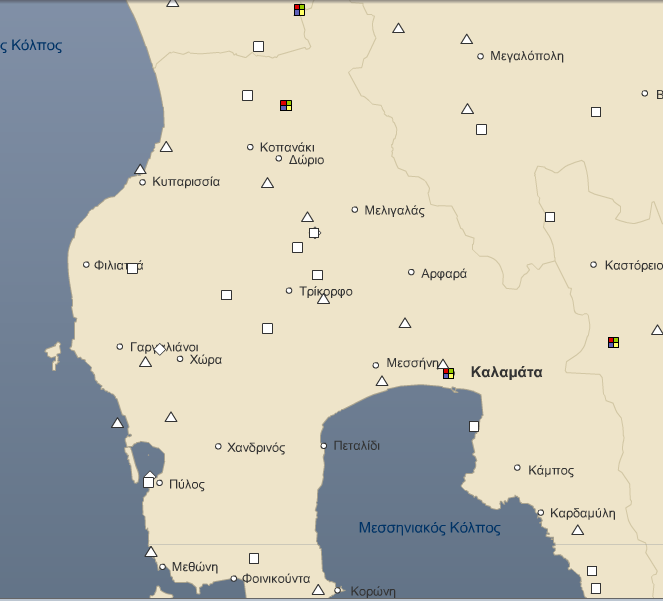
\includegraphics [scale = 0.60] {messinia2.png}
			\caption{Πολιτιστική κληρονομιά Μεσσηνίας}
		\end{center}
	\end{figure}

	\underline{Υπόμνημα}
	
	\begin{figure} [H]
		\begin{center}
			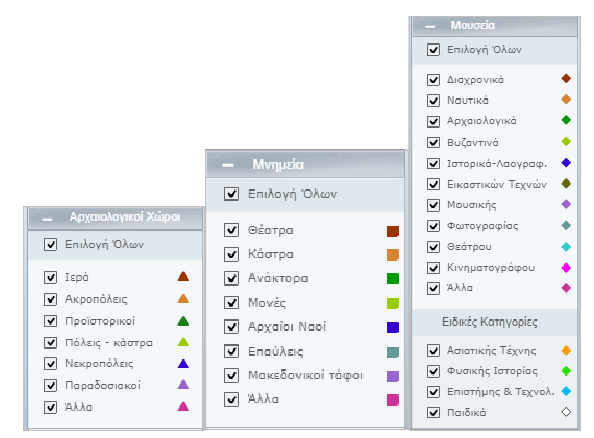
\includegraphics [scale = 0.60] {ypomnima.png}
			\caption{Υπόμνημα}
		\end{center}
	\end{figure}

	\begin{figure} [H]
		\begin{center}
			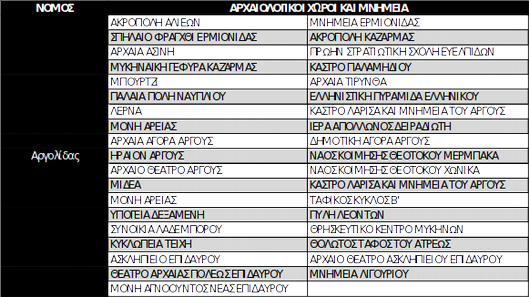
\includegraphics [scale = 1] {argolida3.png}
			\caption{Αρχαιολογικοί χώροι και μνημεία Αργολίδας}
		\end{center}
	\end{figure}
	
	\begin{figure} [H]
		\begin{center}
			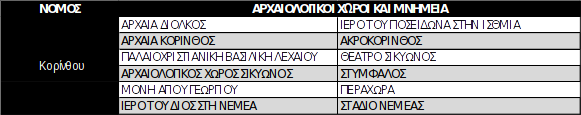
\includegraphics [scale = 0.92] {korinthia3.png}
			\caption{Αρχαιολογικοί χώροι και μνημεία Κορινθίας}
		\end{center}
	\end{figure}

	\begin{figure} [H]
		\begin{center}
			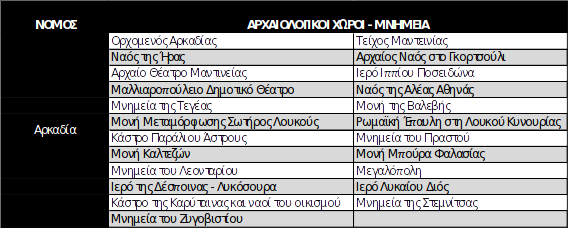
\includegraphics [scale = 0.95] {arkadia3.png}
			\caption{Αρχαιολογικοί χώροι και μνημεία Αρκαδίας}
		\end{center}
	\end{figure}

	\begin{figure} [H]
		\begin{center}
			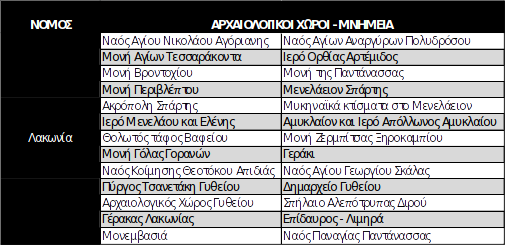
\includegraphics [scale = 1.1] {lakonia3.png}
			\caption{Αρχαιολογικοί χώροι και μνημεία Λακωνίας}
		\end{center}
	\end{figure}

	\begin{figure} [H]
		\begin{center}
			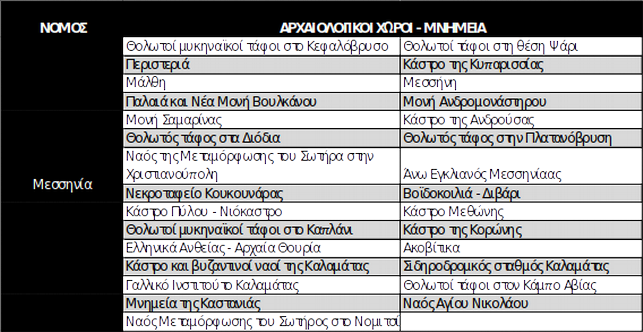
\includegraphics [scale = 0.90] {messinia3.png}
			\caption{Αρχαιολογικοί χώροι και μνημεία Μεσσηνίας}
		\end{center}
	\end{figure}
	
	\subsection{1η Υποενότητα}
	\subsubsection{Φυσικό Περιβάλλον}
	
	\paragraph{Ανάγλυφο}
	
	\textbf{Γεωγραφία}
	
	Ο νομός Αργολίδας  βρίσκεται στο ανατολικό τμήμα της Πελοποννήσου έχει έκταση 2.154 τ.χλμ., 97.044 κατοίκους (απογραφή ΕΛΣΤΑΤ 2011) και πρωτεύουσα το Ναύπλιο. Στα βόρεια συνορεύει με  το νομό Κορινθίας και στα δυτικά και νότια με το νομό Αρκαδίας. Βρέχεται στα νοτιοανατολικά από τον Αργολικό κόλπο, στα βορειοανατολικά από τον Σαρωνικό και αποτελεί μέρος με αξιοσημείωτη πολιτιστική κληρονομιά. Απαρτίζεται από τέσσερις δήμους, οι οποίοι είναι οι εξής:
	
	\begin{table}[H]
		\centering
		\label{my-label}
		\begin{tabular}{|c|c|}
			\hline
			\textbf{A/A} & \textbf{Δήμος}   \\ \hline
			1            & Άργους - \\ 
						& Μυκηνών \\ \hline
			2            & Επιδαύρου        \\ \hline
			3            & Ερμιονίδας       \\ \hline
			4            & Ναυπλιέων       \\ \hline
		\end{tabular}
	\caption{Δήμοι Νομού Αργολίδας}
	\end{table}
	
	Ο νομός Κορινθίας τοποθετείται στο βόρειο και ανατολικό άκρο της Πελοποννήσου, με έκταση 2.290 τ.χλμ, πληθυσμό 145.082 κατοίκους (απογραφή ΕΛΣΤΑΤ 2011) και πρωτεύουσα την ομόνυμη Κόρινθο. Συνορεύει ανατολικά με τον νομό Αχαΐας και νότια κατά κύριο λόγο με τον Ν. Αργολίδας κι ένα μικρό τμήμα της με τον Ν. Αρκαδίας. Ένα κομμάτι της εδαφικά βρίσκεται στη Στερεά Ελλάδα και τα σύνορά της βόρεια και ανατολικά αφορούν σε δύο κόλπους, τον Σαρωνικό και τον Κορινθιακό αντίστοιχα. Ακόμη περιλαμβάνει στα όριά της ένα από τα σημαντικότερα στρατηγικά σημεία της Ελλάδας, όπως είναι η διώρυγα του Ισθμού. Ο νομός διαθέτει συνολικά έξι δήμους, οι οποίοι είναι:
	
	\begin{table}[H]
		\centering
		\label{my-label}
		\begin{tabular}{|c|c|}
			\hline
			\textbf{A/A} & \textbf{Δήμος}   \\ \hline
			1            & Βέλου – Βόχας \\ \hline
			2            & Κορινθίων        \\ \hline
			3            & Λουτρακίου \\
						& Αγίων Θεοδώρων \\
						& Περαχώρας      \\ \hline
			4            & Νεμέας       \\  \hline
			5			& Ξυλοκάστρου \\
						& Ευρωστίνης \\  \hline
			6			& Σικυωνιών \\ \hline
		\end{tabular}
		\caption{Δήμοι Νομού Κορινθίας}
	\end{table}
	
	Ο νομός Αρκαδίας καταλαμβάνει το κέντρο της Πελοποννήσου. Συνορεύει βόρεια με τους νομούς Κορινθίας και Αχαΐας, δυτικά με τους νομούς Ηλείας και Μεσσηνίας, νότια με το νομό Λακωνίας και ανατολικά βρέχεται από τον Αργολικό κόλπο. Έχει έκταση 4.419 τετραγωνικά χιλιόμετρα και πληθυσμό 102.035\footnote{Σύμφωνα με τα αποτελέσματα της απογραφής του 2001} κατοίκους. Αποτελεί το διοικητικό κέντρο της περιφέρειας Πελοποννήσου με τις περισσότερες από τις υπηρεσίες της να βρίσκονται στην πρωτεύουσα του νομού, την Τρίπολη. Έχει μεγάλη ιστορική σημασία, και οι πέντε δήμοι στους οποίους διακρίνεται είναι:
	
	\begin{table}[H]
		\centering
		\label{my-label}
		\begin{tabular}{|c|c|}
			\hline
			\textbf{A/A} & \textbf{Δήμος}    \\ \hline
			1            & Βόρειας Κυνουρίας  \\ \hline
			2            & Γορτυνίας          \\ \hline
			3          	 & Μεγαλόπολης        \\ \hline
			4            & Νότιας Κυνουρίας   \\  \hline
			5			 & Τρίπολης \\ \hline
		\end{tabular}
		\caption{Δήμοι Νομού Αρκαδίας}
	\end{table}
	
	Τρεις από τους συνολικά πέντε δήμους της ανήκουν στην πρώτη υποενότητα και δεν είναι άλλοι από τους δήμους Βόρειας Κυνουρίας, Νότιας Κυνουρίας και Τρίπολης, στα βόρεια, νότια και ανατολικά του νομού.
	
	Όσον αφορά τη γεωμορφολογία της Αργολίδας (βλ. σελίδα \pageref{peloponnese}), διαθέτει κυρίως ορεινό έδαφος με εξαίρεση την κλειστή πεδιάδα του Άργους - η οποία διαβρέχεται από τον μοναδικό ποταμό, τον Ερασινό – και μερικές παράκτιες μικρές πεδιάδες, όπως αυτές του Κρανιδίου και της Ερμιόνης, καθώς και την κοιλάδα του Λυγουριού. Σημαντικά όρη που μαρτυρούν το ανάγλυφό της αυτό είναι το Αραχναίο (1.197 μ.), το Αρτεμίσιο (1.771 μ.) που αποτελεί και το υψηλότερο βουνό του νομού, το Μεγαλοβούνι (1.272 μ.), Τραπεζώνα (1.137 μ.), Δίδυμο (1.121 μ.) και Φαρμακάς (1.617 μ.). Χαρακτηριστικοί είναι επίσης και οι χείμαρροι που απαντώνται στην περιοχή και εκβάλλουν στον Αργολικό Κόλπο, όπως ο Χάραδρος (Ξεριάς), ο Ίναχος και ο Σέλλας.
	
	Ο νομός Κορινθίας ακολουθεί περίπου το ίδιο μορφολογικό μοντέλο με εκείνο της Αργολίδας, μιας και το 60\% περίπου ανήκει στην ορεινή ζώνη, και το υπόλοιπο 40\% κατανέμεται σχεδόν ισόποσα στην ημιορεινή και πεδινή της ζώνη. Στην δυτική της πλευρά συγκεντρώνεται το μεγαλύτερο ποσοστό ορεινών μαζών, με κυριότερο αυτόν της Κυλλήνης (Ζήριας) στα 2.376 μ. Επίσης, στα σύνορα Κορινθίας-Αρκαδίας-Αργολίδας τοποθετείται το όρος Ολίγυρτος με υψηλότερη κορυφή στα 1.853 μ. Άλλοι ορεινοί όγκοι που έχουν καταγραφεί στην περιοχή με φθίνουσα σειρά υψομέτρου είναι η Παράγκα (2.036 μ.), ο Σαϊτάς (1.814 μ.), το Γερόντιο Όρος (1.756 μ.), το Μαύρο Όρος (1.757 μ.), η Ευρωστίνα (1.208), ο Γαβριάς (1.209 μ.) και τα Γεράνεια Όρη (με κορυφές Μακρυπλάγι 1.351 μ. και Πίντιζα 1.032 μ.). Το πεδινό της τμήμα, από την άλλη, απαρτίζεται κυρίως από τον κάμπο της Κορίνθου, ο οποίος και βρέχεται από χειμαρροπόταμους και ρέματα, μιας και στον νομό δεν υπάρχουν ποταμοί. Το μοναδικό ρέμα που έχει καταγραφεί ως ποταμός είναι ο Ασωπός, που πηγάζει από τον ορεινό όγκο Φαρμακά (Ν. Αργολίδας)και εκβάλλει ανατολικά του Κιάτου στον Κορινθιακό Κόλπο. Ωστόσο, παρά την απουσία συνεχούς ροής η Κορινθία διαθέτει τρεις τύπους υγροτόπων, όπως το έλος του Λεχαιού, την τεχνητή λίμνη του αρδευτικού φράγματος Δόξας Φενεού και την φυσική λίμνη Στυμφαλία, η οποία εντάσσεται και στο δίκτυο προστατευόμενων περιοχών \selectlanguage{english}Natura 2000.
	
	\selectlanguage{greek}Στο νομό Αρκαδίας, επίσης, η ανάγλυφη όψη του παρουσιάζεται ως ορεινή με κύρια χαρακτηριστικά τους ορεινούς όγκους που διακόπτονται από μικρές κοιλάδες και οροπέδια. Στο κέντρο περίπου της Αρκαδίας απλώνεται το οροπέδιο της Τρίπολης που περιβάλλεται από τα Αργολιδοαρκαδικά όρη και τις βόρειες προεκτάσεις του Πάρνωνα και από όπου πηγάζει ο ποταμός Αλφειός. Αξιοσημείωτα βουνά του οροπεδίου είναι το Μαίναλο (1.981 μ.), ο Αλωνίσταινας (1.859 μ.), ο Ολίγυρτος (Σκίπιζα 1.935 μ.), το Αρτεμίσιο (1.771 μ.), το Αφροδίσιο (1.456 μ.), το Δρακοβούνι (1.077 μ.), το Παρθένιο (1.215 μ.), το Γκρεκόζι (1.697 μ.), το Λύρκειο (1.648 μ.), ο Κτενίας (1.598 μ.) και η Μίνθη (Κουκούβερο 1.296 μ.).
	
	Ως σημαντικότερος ποταμός χαρακτηρίζεται  ο Αλφειός που πηγάζει από τα οροπέδια της Μεγαλόπολης και στον οποίο εκβάλλει ο ποταμός Ερύμανθος (Αχαΐα). Πολλοί ποταμοί της Αρκαδίας αποτελούν παραπόταμοι του Αλφειού, όπως για παράδειγμα ο Βουφάγος, Ελισσώνας, Ξερίλας, Λούσιος. Αξιοσημείωτος είναι και  ο ποταμός Λάδωνας που πηγάζει από καρστικές πηγές στα βόρεια του νομού. Όσον αφορά τις λίμνες της περιοχής, αυτές είναι η λίμνη Τάκα (υδροβιότοπος της Πελοποννήσου) και η τεχνητή λίμνη του Λάδωνα που δημιουργήθηκε έπειτα από κατασκευή φράγματος στον ομώνυμο ποταμό. 
	
	\textbf{Ακτογραφία}
	
	Κύριο χαρακτηριστικό της ακτογραφίας της πρώτης υποενότητας αποτελούν οι κόλποι (βλ. σελίδα \pageref{peloponnese}). Συγκεκριμένα, ο Ν. Κορινθίας και ο Ν. Αργολίδας περιβάλλονται από τον Σαρωνικό και τον Αργολικό Κόλπο. Ο Σαρωνικός  αποτελεί εγκόλπωση του Αιγαίου που ορίζεται βόρεια από τις ακτές της Αττικής, βορειοδυτικά και δυτικά από τις ακτές του Ν. Κορινθίας και νοτιοδυτικά από τις ακτές του Ν. Αργολίδος. Συνδέει μέσω του Ισθμού της Κορίνθου το Αιγαίο με το Ιόνιο πέλαγος και διαθέτει απότομο  ανάγλυφο, λόγω μεγάλων παραποτάμιων αποθέσεων. Ο Αργολικός Κόλπος τοποθετείται μεταξύ της Αργολικής χερσονήσου και των ανατολικών παραλίων της Αρκαδίας και της Λακωνίας. Οι ακτές του είναι απόκρημνες στο τμήμα της νότιας Αργολίδας και Αρκαδίας και ομαλές στην βόρεια πλευρά του, που συναντά τον αργολικό κάμπο. Στον κόλπο αυτόν προβάλλει και τμήμα της Αρκαδίας που ανήκει στην 1η υποενότητα, παρόλο που κατά κύριο λόγο περιβάλλεται από στεριά κι όχι από θάλασσα.
	
	 Η ακτογραμμή της πρώτης υποενότητας ξεκινά από το Λεωνίδιο του Νομού Αρκαδίας και συνεχίζει βόρεια διαγράφοντας τον Αργολικό κόλπο. Λίγο πριν συναντήσει το Ναύπλιο ξεκινά την κίνηση προς τα νότια, οπότε παρουσιάζει έντονες εγκολπώσεις. Στο νοτιότερο άκρο του νομού Αργολίδας διασταυρώνεται με το Πόρτο Χέλι και τη νήσο Σπέτσες και στη συνέχεια συνεχίζοντας προς τα βορειοανατολικά δημιουργεί τον κόλπο της Ύδρας που συνδέει τη νήσο Ύδρα με το ηπειρωτικό κομμάτι του Νομού. Στο σημείο αυτό η ακτογραμμή κινείται προς τα βόρεια και συναντά τα εξογκώματα του Πόρου και των Μεθάνων. Στο σημείο αυτό ξεκινά ο Σαρωνικός κόλπος. Η ακτογραμμή διαγράφει το Νομό Κορινθίας και αφού συναντήσει την Επίδαυρο παρουσιάζει μια έντονη εγκόλπωση στον Ισθμό της Κορίνθου και καταλήγει στους Αγίους Θεοδώρους. Στο βόρειο τμήμα της πρώτης υποενότητας η ακτογραμμή σχηματίζει τον Κορινθιακό κόλπο ξεκινώντας από τον Ισθμό και καταλήγοντας στο Ξυλόκαστρο.  
	 
	 \paragraph{Έδαφος-Γεωλογία-Υδατικοί πόροι}
	 
	 \textbf{Έδαφος}
	 
	 Σύμφωνα με την ταξινόμηση των εδαφών (βλ. σελίδα \pageref{edafidafi}), βάσει του συστήματος \selectlanguage{english}FAO \selectlanguage{greek}(Χάρτης Εδαφών Ελλάδας – Εθνική Επιτροπή κατά της Ερημοποίησης – Γεωπονικό Πανεπιστήμιο Αθηνών – Συντάκτης Ν. Γιάσογλου – ( Παράρτημα IΙ ), τα εδάφη της Περιφέρειας Πελοποννήσου ταξινομούνται σε επτά κατηγορίες εδαφών, οι οποίες είναι:
	 
	 \begin{itemize}
	 	\item \emph{Βράχοι}(Rock Outcrops) (μαύρο χρώμα)
	 	\item \emph{\selectlanguage{english}Leptosols}\selectlanguage{english}(LP): \selectlanguage{greek}Εδάφη με μητρικό υλικό από ασβεστόλιθο και φλύσχη. Είναι λεπτόκοκκα εδάφη, αργιλώδη, καλής υδατοπερατότητας με ουδέτερο \selectlanguage{english}pH. \selectlanguage{greek}(γκρι χρώμα)
	 	\item \emph{\selectlanguage{english}Regosols}\selectlanguage{english}(RG): \selectlanguage{greek}Στρώμα χαλαρού υλικού, πάνω σε σκληρό υπόβαθρο. Είναι εδάφη μετρίως αργιλώδη, με μέτρια υδατοπερατότητα και με \selectlanguage{english}pH $>$ 7.\selectlanguage{greek}(κίτρινο χρώμα)
	 	\item \emph{\selectlanguage{english}Fluvisols}\selectlanguage{english}(FL): \selectlanguage{greek}Εδάφη αργιλώδη, με μέτρια έως μικρή υδατοπερατότητα και με \selectlanguage{english}pH $>$ 7.\selectlanguage{greek}(μπλε χρώμα)
	 	\item \emph{\selectlanguage{english}Cambisols}\selectlanguage{english}(CM): \selectlanguage{greek}Η σύσταση των εδαφών αυτών είναι αργιλλώδης και μετρίως αργιλλώδης, με μικρή υδατοπερατότητα και με ουδέτερο ή ελαφρώς όξινο \selectlanguage{english}pH. \selectlanguage{greek}(πορτοκαλί χρώμα)
	 	\item \emph{\selectlanguage{english}Luvisols}\selectlanguage{english}(LV): \selectlanguage{greek}Τα εδάφη αυτά είναι αργιλώδη με υψηλή υδατοπερατότητα και με \selectlanguage{english}pH $\approx$ 7.\selectlanguage{greek}(ροζ χρώμα)
	 \end{itemize}
 
 	Στο νότιο τμήμα της Κορινθίας τα εδάφη είναι αργιλώδη μεγάλης υδατοπερατότητας και ουδέτερου \selectlanguage{english}pH, \selectlanguage{greek}ενώ στο βόρειο τμήμα η υδατοπερατότητα περιορίζεται αρκετά και το \selectlanguage{english}pH \selectlanguage{greek}είναι αλκαλικό εκτός από ένα κομμάτι βόρεια του όρους Κυλλήνη, όπου είναι όξινο.
 	
 	Στην Αργολίδα τα εδάφη είναι αργιλώδη με μέτρια έως μικρή υδατοπερατότητα και ουδέτερο έως αλκαλικό pH στα νότια και όξινο pH στο βόρειο τμήμα του Νομού.
 	
 	Τα εδάφη της Αρκαδίας είναι σε γενικές γραμμές αργιλώδη, αργιλοπηλώδη, πηλώδη και αμμοαργιλοπηλώδη. Έχουν μικρή περιεκτικότητα σε άλατα (0,01\%) και το \eng pH \gr τους είναι κατάλληλο για καλλιέργεια. Ωστόσο, μεγάλο κομμάτι της καταλαμβάνεται από όρη και λόφους, γι αυτό θεωρείται κυρίως ορεινό. 
 	
 	Όπως φαίνεται στο χάρτη δυνητικού κινδύνου ερημοποίησης της Ελλάδας (βλ. σελίδα \pageref{erimopoiisi}) που συνετάχθη από την Εθνική Επιτροπή κατά της Ερημοποίησης, το έδαφος της πρώτης υποενότητας κατατάσσεται ως μετρίου κινδύνου στην περιοχή της Κορινθίας και υψηλού κινδύνου στην περιοχή της Αρκαδίας και Αργολίδας.
 	
 	\textbf{Γεωλογία-Τεκτονική}
 	
 	Όπως φαίνεται στο γεωτεκτονικό χάρτη της Πελοποννήσου (βλ. σελίδα \pageref{geotektonikes}) οι γεωτεκτονικές ζώνες που εμφανίζονται στην πρώτη υποενότητα είναι οι εξής:
 	
 	\begin{enumerate}
 		\item \textbf{Ζώνη Ολωνού-Πίνδου} \\
 		Κατέχει κεντρική θέση στον κορμό της Ελλάδας και ακολουθεί την κάμψη του ορογενετικού τόξου, ενώ τμήματα της απαντούν στην Κρήτη και τη Ρόδο. Συνίσταται από ασβεστόλιθους, δολομίτες, κερατόλιθους, ηφαιστειοϊζηματογενή πετρώματα, ραδιολαρίτες, αργίλους, ψαμμίτες και πηλίτες. Έχει επωθηθεί προς τα δυτικά πάνω στη ζώνη Γαβρόβου-Τριπόλεως και χαρακτηρίζεται από δομή λεπίων, με αποτέλεσμα συχνές επαναλήψεις των στρωμάτων. Πάνω στη ζώνη της Πίνδου βρίσκονται επωθημένες οι μεγαλύτερες οφιολιθικές μάζες του ελληνικού χώρου.
 		\item \textbf{Ζώνη Γαβρόβου-Τριπόλεως} \\
 		Η ζώνη Γαβρόβου - Τριπόλεως χαρακτηρίζεται από συνεχή ανθρακική ιζηματογένεση με κυρίαρχα πετρώματα τους ασβεστόλιθους και δολομίτες. Οι σχηματισμοί της ζώνης αυτής επικάθονται σε ένα υπόβαθρο αποτελούμενο από φυλλίτες, χαλαζιακούς φυλλίτες και μάρμαρα, γνωστό ως «φυλλιτική-χαλαζιτική» σειρά. Τα στρώματά της σχηματίζουν μεγάλα ανοικτά σύγκλινα και αντίκλινα και είναι επωθημένη δυτικά πάνω στην Ιόνιο ζώνη.
 		\item \textbf{Πελαγονική Ζώνη} \\
 		Η Πελαγονική ζώνη κατέχει ένα μεγάλο τμήμα του κορμού της Ελλάδας και αποτελείται από ένα κρυσταλλοσχιστώσες υπόβαθρο (γνεύσιους, γνευσιοσχιστόλιθους και  αμφιβολίτες με μεγάλες γρανιτικές διεισδύσεις), μάρμαρα, φυλλίτες, σχιστόλιθους, ψαμμίτες, ασβεστόλιθους και δολομίτες. Χαρακτηριστική είναι η ύπαρξη τεκτονικά τοποθετημένων μεγάλων οφιολιθικών μαζών. Διακρίνεται στην Πελαγονική ζώνη  μεταμορφωμένων σχηματισμών (όπου εμφανίζονται αποκλειστικά μεταμορφωμένα πετρώματα) και την Πελαγονική ζώνη μη μεταμορφωμένων σχηματισμών (ή Υποπελαγονική).
 		\item \textbf{Ζώνη Παρνασσού-Γκιώνας} \\
 		Η ζώνη αυτή έχει περιορισμένη έκταση στην Κεντρική Ελλάδα και αποτελείται σχεδόν αποκλειστικά από ασβεστόλιθους και δολομίτες, με βασικό χαρακτηριστικό την ύπαρξη τριών  βοξιτικών οριζόντων. (Σημειώνεται ότι οι βωξίτες αποτελούσαν για δεκαετίες σημαντικό παράγοντα για την οικονομία της χώρας). Απουσιάζουν εντελώς τα μαγματικά πετρώματα. Βρίσκεται απωθημένη προς τα δυτικά πάνω στη ζώνη της Πίνδου.
 	\end{enumerate}
 
 	\textbf{Υδάτινο Περιβάλλον}
 	
 	Η Δ.Ε. που εξετάζεται ανήκει και στα τρία υδατικά διαμερίσματα (βλ. σελίδα \pageref{ydatika}). Όσον αφορά το υδατικό διαμέρισμα Δυτικής Πελοποννήσου-στο οποίο εντάσσεται κατά το ήμισυ η Π.Ε. Αρκαδίας- αποτελείται από τις εξής λεκάνες απορροής Αλφειού \eng(GR29)\gr έκτασης 3. 658 $km^2$ και Πάμισου – Νέδοντος – Νέδα \eng(GR32)\gr έκτασης 3.425 $km^2$. Η  οριοθέτηση του Διαμερίσματος αυτού γίνεται από τον υδροκρίτη του, όπως ορίζεται ανατολικά από το Μαίναλο και τον Ταΰγετο και βόρεια από τους ορεινούς όγκους Ερύμανθου και Αροανείων. 
 	
 	Η Π.Ε. Κορινθίας υπάγεται κατά κύριο λόγο στο Υδατικό Διαμέρισμα Βόρειας Πελοποννήσου που αποτελείται από τις Λεκάνες Απορροής Πείρου – Βέργα – Πηνειού \eng(GR28)\gr έκτασης 2.423 $km^2$, Ρεμάτων Παραλίας Β. Πελοποννήσου \eng(GR27)\gr 3.685 $km^2$ και Κεφαλονιάς – Ιθάκης – Ζακύνθου \eng(GR45)\gr 1.310 $km^2$. Το Υδατικό αυτό Διαμέρισμα  οριοθετείται στο χερσαίο τμήμα του από τον υδροκρίτη  που ξεκινά από το ακρωτήριο Κατάκολο, συνεχίζει στους ορεινούς όγκους Φολόη, Λάµπεια, Ερύµανθο, Αροάνεια, στο υψίπεδο Καλαβρύτων, στο νότιο όριο της κλειστής λεκάνης Φενεού, στους ορεινούς όγκους του Ολίγυρτου, Λύρκειου και Ονείων, και καταλήγει στο ακρωτήριο Τραχήλι µέσω των κορυφών Τραπεζώνα και Πολίτη στην Κορινθία.
 	
 	Η Π.Ε. Αργολίδας περιλαμβάνεται εξ ολοκλήρου γεωγραφικά από το Υδατικό Διαμέρισμα Ανατολικής Πελοποννήσου, το οποίο αποτελείται από τις Λεκάνες Απορροής του Οροπεδίου Τρίπολης \eng(GR30)\gr έκτασης 907 $km^2$, των Ρεμάτων Αργολικού Κόλπου \eng(GR31)\gr έκτασης 5.796 $km^2$ και Ευρώτα \eng(GR33)\gr έκτασης 2.239 $km^2$. Όσον αφορά στα φυσικά-γεωμορφολογικά όρια του Διαμερίσματος, αυτά είναι προς τα δυτικά ο Ταΰγετος και το Μαίναλο, προς τα βόρεια ο ορεογραφικός άξονας Ολύγιρτου-Λυρκείων – Ονείων, προς τα ανατολικά ο Πάρνωνας, ο Αργολικός Κόλπος και ο Κόλπος της Επιδαύρου και προς τα νότια ο Λακωνικός Κόλπος.
 	
 	Πλήθος υπόγειων υδάτων παρατηρείται στην περιοχή της ανατολικής Αρκαδίας και στο μεγαλύτερο μέρος της Αργολίδας (βλ. σελίδα \pageref{ypogeia}). Παρά το μικρό ύψος βροχής που εμφανίζεται στην περιοχή, τα μεγάλα αποθέματα της Αργολίδας οφείλονται στον Αργολικό κάμπο, που έχει γεωλογικούς σχηματισμούς μεγάλης αποθηκευτικής ικανότητας. Όμως, η εντατική εκμετάλλευση των υπογείων νερών με πηγάδια και γεωτρήσεις για την άρδευση των καλλιεργειών, είχε σαν αποτέλεσμα τη σημαντική ταπείνωση της στάθμης του υδροφορέα, με συνέπεια τη διείσδυση της θάλασσας στα υπόγεια νερά και την υποβάθμιση της ποιότητάς τους, λόγω αύξησης των χλωριόντων (υφαλμύρωση). Το φαινόμενο αυτό γίνεται πιο έντονο σε παράκτιες περιοχές με ιδιαίτερα εντατικές καλλιέργειες (Ίρια, Ν. Κίο, Ασίνη, Τολό, Δρέπανο κ.ά.). Ένα τμήμα υπόγειων νερών διαθέτει και η Κορινθία στην κομμάτι γύρω από την περιοχή του Ισθμού, σύμφωνα με τον χάρτη.
 	
 	\paragraph{Σεισμική Επικινδυνότητα}
 	
 	Η σεισμικότητα μιας περιοχής εξαρτάται άμεσα από τους γεωλογικούς σχηματισμούς που εμφανίζονται σε αυτή. Σύμφωνα με τον εθνικό χάρτη σεισμικής επικινδυνότητας (βλ. σελίδα \pageref{seismiki}) η Ελλάδα χωρίζεται σε τρεις ζώνες σεισμικής επικινδυνότητας, αλλά στην Πελοπόννησο (και στην 1η Δ.Ε.) εμφανίζονται μόνο η Ζώνη Ι επιτάχυνσης σχεδιασμού \eng0,16g\gr και η Ζώνη ΙΙ \eng(0,24 g)\gr. Ο Ν. Κορινθίας χαρακτηρίζεται από έντονη σεισμική δράση και αποτελεί μια από τις δύο σημαντικότερες σεισμογενείς περιοχές της Περιφέρειας, κυρίως λόγω ενεργών ρηγμάτων που βρίσκονται στη θέση του Κορινθιακού Κόλπου (Ζώνη ΙΙ). Τέτοια είναι το ρήγμα Σχοίνου και Πισίων, Λουτρακίου, Αγίων Θεοδώρων, Κεχραιών, Μύλου και Κατακαλίου. Οι άλλοι δύο νομοί δεν εμφανίζουν ιδιαίτερη σεισμική δραστηριότητα. Όμως οι σεισμοί στην Αρκαδία είναι μικρού σεισμικού βάθους και κατ’ επέκταση μεγάλων μακροσεισμικών εντάσεων.
 	
 	Ως προς τον κίνδυνο κατολίσθησης (βλ. σελίδα \pageref{katolisthiseis}) το σύνολο της πρώτης υποενότητας κατατάσσεται στις ζώνες χαμηλής έως μηδαμινής επικινδυνότητας.
 	
 	\paragraph{Οικότοποι-Χλωρίδα-Πανίδα}
 	
 	\textbf{Τύποι Οικοσυστημάτων}
 	
 	Οι τύποι οικοσυστημάτων που εμφανίζονται στην πρώτη διαχειριστική ενότητα αφορούν σε υγροτόπους, παράκτια οικοσυστήματα, σπήλαια, δασικά και αγροτικά οικοσυστήματα.
 	
 	\textbf{Χλωρίδα-Πανίδα} 
 		
		\emph{Αργολίδα} \\
		Το μεγαλύτερο ποσοστό των δασικών της εκτάσεων καλύπτεται από θαμνώδη βλάστηση, κυρίως πουρνάρια. Από τα ΝΑ προς τα ΒΔ καταγράφεται η  εμφάνιση πλατύφυλλων όπωα η Κουμαριά και ο Κέδρος. Τα παράλια των επαρχιών Ναυπλίου και Ερμιονίδος χαρακτηρίζονται από την εμφάνιση της Χαλεπείου Πεύκης, ενώ στην ορεινή Αργολίδα επικρατεί η Υβριδογενής Ελάτη (Κεφαλληνιακή). Ένα μικρό κομμάτι πευκοδάσους απαντάται στο Κεφαλάρι (Άργος) κοντά στις πηγές του Ερασινού, όμως οι υπόλοιπες μή καλλιεργούμενες εκτάσεις εμφανίζουν χαμηλή βλάστηση. 
		
		\emph{Κορινθία} \\
		Στο νομό παρατηρούνται αμιγή δάση κεφαλληνιακής ελάτης στους ορεινούς όγκους του Ολίγυρτου, του Χελμού, της Λέχωβας, στους βόρειους πρόποδες της Ζήρειας και την κορυφή των Γερανείων. Αμιγή δάση χαλεπίου πεύκης αναπτύσσονται στους ορεινούς όγκους των Γερανείων, της χερσονήσου της Σολυγείας, τις περιοχές του Χιλιομοδίου, Αθικίων και στην ημιορεινή παράλληλη ζώνη της κεντρικής και δυτικής Κορινθίας. Επιπλέον, αμιγή δάση μαύρης πεύκης εντοπίζονται στους βόρειους πρόποδες της Ζήρειας, το Μαύρο όρος και τον Χελμό. Μικτά δάση αείφυλλων - πλατύφυλλων καλύπτουν το 44\% των ορεινών όγκων και αναπτύσσονται κυρίως στις ημιορεινές περιοχές της ανατολικής Κορινθίας. Υπάρχουν και δύο αμιγή δάση δρυός (βελανιδιάς) στο νομό, του Σπαρτιά και του Μουγγοστού που έχει κηρυχθεί και Αισθητικό Δάσος, καθώς επίσης και ο Πευκιάς του Ξυλοκάστρου.
		
		\emph{Αρκαδία} \\
		Η Αρκαδία διαθέτει αρκετά δάση από φυλλοβόλα δέντρα, όπως είναι η οξιά και η φυλλοβόλα δρύς. Στις ημιορεινές περιοχές της συναντάται η χαλέπιος πεύκη, η οποία είναι ανθεκτική στις δύσκολες καιρικές συνθήκες. Ακόμη, εντοπίζονται πολλά και διαφορετικά είδη δέντρων και χαμηλή βάστησης, όπως  είναι η μαύρη πεύκη, η καστανιά, τα πλατάνια, η ασημοϊτιά, το δεδρόκεδρο κ.ά.
		
		Ως προς τη πανίδα της υποενότητας αυτής, στα ορεινά ζουν και αναπτύσσονται μικρού ή μεσσαίου μεγέθους θηλαστικά, όπως είναι ο λαγός, η αλεπού, το τσακάλι, το κουνάβι, η νυφίτσα κ.ά. Στους υγροτόπους της περιοχής εμφανίζεται πληθώρα υδρόβιων πτηνών (π.χ. κύκνοι, αγριόπαπιες), καθώς και ποικιλία αμφιβίων και ερπετών. Τέλος, στις παράκτιες περιοχές εντοπίζεται μεγάλος αριθμός θαλάσσιων πουλιών, με κύριο είδος τους πελαργούς και τα θαλασσοπούλια.

	\textbf{Ευαίσθητες και Προστατευόμενες περιοχές}
	
	\underline{\eng Natura 2000}\gr
	
	\begin{table}[H]
		\centering
		\begin{tabular}{|c|c|}
			\hline
			\multicolumn{2}{|c|}{\textbf{\eng NATURA 2000}} \\ \hline
			\textbf{\gr ΚΩΔΙΚΟΣ} & \textbf{ΟΝΟΜΑ} \\ \hline
			\eng GR2510003 & \gr Ακροναυπλία-Παλαμήδι \\ \hline
			\eng GR2410004 & \gr Όρη Αρτεμήσιο και Λύρκειο \\ \hline
			\eng GR2520001 & \gr Όρος Μαίναλο \\ \hline
			\eng GR2520002 & \gr Λίμνη Τάκα \\ \hline
			\eng GR2520003 & \gr Λιμνοθάλασσα Μουστού \\ \hline
			\eng GR2520005 & \gr Μονή Ελώνας και Χαράδρα Λεωνιδίου \\ \hline
			\eng GR2520006 & \gr Όρος Πάρνωνας \\ \hline
			\eng GR2530001 & \gr Κορυφές όρους Κυλλήνη (Ζήρεια)- \\
			& Χαράδρα Φλαμπουρέτσα \\ \hline
			\eng GR2530002 & \gr Λίμνη Στυμφαλία \\ \hline
			\eng GR2530003 & \gr Ακροκόρινθος \\ \hline
			\eng GR2530004 & \gr Όρος Ολίγυρτος \\ \hline
			\eng GR2530005 & \gr Όρη Γεράνεια \\ \hline
			\eng GR2530006 & \gr Όρη Ζήρεια \\ \hline
		\end{tabular}
	\caption{\eng Natura 2000} \gr
	\label{The label}
	\end{table}
	
	\underline{Καταφύγια άγριας ζωής}
	
	\begin{table}[H]
		\centering
		\begin{tabular}{|c|c|}
			\hline
			\multicolumn{2}{|c|}{\textbf{ΚΑΤΑΦΥΓΙΑ ΑΓΡΙΑΣ ΖΩΗΣ}} \\ \hline
			\textbf{Α/Α} & \textbf{ΟΝΟΜΑ} \\ \hline
			Κ438 & Πρ. Ηλίας-Δελόκορμο (Μυκήνες) \\ \hline
			Κ446 & Μάλιζα-Τουρνέζα \\ \hline
			Κ458 & Νησίδες Ρόμβη-Δασκαλειό \\ \hline
			Κ707 & Κυνόρτιο  Όρος \\ \hline
			Κ457 & Σταυροπόδι-Καναρπίτσα \\ \hline
			Κ815 & Κάμπος Κρανιδίου \\ \hline
			Κ456 & Δασώδης Περιοχή Αγ. Θεοδώρων \\ \hline
			Κ709 & Υγροβιότοπος Μουστού \\ \hline
			Κ469 & Μονή Παλαιοπαναγιάς \\ \hline
			Κ710 & Κορομηλιά Λεωνιδίου \\ \hline
			Κ725 & Φαράγγι Μαζιάς \\ \hline
			Κ472 & Φονεμένοι Κυνουρίας \\ \hline
			Κ889 & Μπούτσι Ξυλοκάστρου \\ \hline
			Κ421 & Γκράβα-Λάκκα \\ \hline
			Κ807 & Λίμνη Στυμφαλία \\ \hline
			Κ417 & Γεράνεια (Λουτρακίου-Περαχώρας) \\ \hline
			Κ590 & Πλάτανος-Μύλοι \\ \hline
		\end{tabular}
		\caption{Καταφύγια Άγριας Ζωής}
	\label{The label}
	\end{table}

	\underline{Τοπία ιδιαίτερου φυσικού κάλλους}
	
	\begin{table}[H]
		\centering
		\begin{tabular}{|c|c|}
			\hline
			\multicolumn{2}{|c|}{\textbf{ΤΟΠΙΑ ΙΔΙΑΙΤΕΡΟΥ ΦΥΣΙΚΟΥ ΚΑΛΟΥΣ}} \\ \hline
			\textbf{ΚΩΔΙΚΟΣ} & \textbf{ΟΝΟΜΑ} \\ \hline
			ΑΤ1011093 & Ακροναυπλί και Παλαμήδι \\ \hline
			ΑΤ1011094 & Ανώνυμος λόφος δυτικά της Ασίνης \\ \hline
			ΑΤ1012001 & Νέα Επίδαυρος \\ \hline
			ΑΤ1011084 & Δημητσάνα, Στεμνίτσα και Φαράγγι Λιουσίου \\ \hline
			ΑΤ1011072 & Καρύταινα \\ \hline
			ΑΤ1010003 & Καστανίτσα Πάρνωνα \\ \hline
			ΑΤ1080115 & ΚΛερασιά-Βλαχοκερασιά Αρκαδίας \\ \hline
			ΑΤ1080128 & Λόφος Στόχος Νεστάνης (Τσιπιανών) \\ \hline
			ΑΤ1011069 & Χώρος Μάχης Βερβαινών \\ \hline
			ΑΤ1011111 & Αισθητικό δάσος Πευκιά Ξυλοκάστρου \\ \hline
			ΑΤ1011006 & Ακροκόρινθος \\ \hline
			ΑΤ1011134 & Βουνό Παναγιάς Κορυφής \\ \hline
			ΑΤ1011001 & Κοιλάδα Φενεού \\ \hline
			AT1011000 & Λόμνη Στυμφαλία \\ \hline
			AT1011095 & Λόφος Παναγιά Κορινθίας \\ \hline
			AT1011002 & Μετέωρα Κορινθίας \\ \hline
			AT1011026 & Μονή Θεοτόκου Περαχώρας \\ \hline
			AT1010006 & Περιοχή Ηραίου Περαχώρας \\ \hline
			AT1011096 & Πέτρα Περαχώρας (Βράχος βουνού) \\ \hline
			AT1011004 & Υψώματα βόρεια του χωριού Κορινθίας \\ \hline
			AT1011135 & Υψώματα Ελληνικού \\ \hline
			AT1011136 & Υψώματα Λυγιάς \\ \hline
		\end{tabular}
		\caption{Τοπία Ιδιαίτερου Φυσικού Κάλλους}
		\label{The label}
	\end{table}
	
	\underline{Βιότοποι \eng Corine\gr}
	
	\begin{table}[H]
		\centering
		\begin{tabular}{|c|c|}
			\hline
			\multicolumn{2}{|c|}{\textbf{ΒΙΟΤΟΠΟΙ \eng CORINE \gr}} \\ \hline
			\textbf{ΚΩΔΙΚΟΣ} & \textbf{ΟΝΟΜΑ} \\ \hline
			A00040053 & Ακροναυπλί και Παλαμήδι \\ \hline
			A00020018 & Έλος χωριού Καντιά \\ \hline
			Α00060086 & Λιμνοθάλασσα Δρεπάνου \\ \hline
			Α00060089 & Λιμνοθάλασσες Θερμησιάς \\ \hline
			Α00060091 & Σπηλιά Φράχτη Ερμιονίδας \\ \hline
			Α00060087 & Υγρότοποι Ερμιονίδας \\ \hline
			Α00060085 & Υγρότοποι τόπου Τολού \\ \hline
			Α00060088 & Υγρότοπος Μετόχι \\ \hline
			Α00060080 & Κορυφές όρους Μαίναλο \\ \hline
			Α00040055 & Κορυφές όρους Πάρνωνα \\ \hline
			Α00010064 & Λίμνη Τάκα \\ \hline
			Α00040056 & Μονή Ελώνας και Χαράδρα Λεωνιδίου \\ \hline
			Α00030044 & Μονή Μαλέβης \\ \hline
			Α00060092 & Όρος Πάρνωνας \\ \hline
			Α00020022 & Ποταμός Λάδων \\ \hline
			Α00010232 & Υγρότοπος Μουστού/Άστρος \\ \hline
			Α00060081 & Φαράγγι Λουσίου \\ \hline
			Α00040052 & Ακροκόρινθος \\ \hline
			Α00030034 & Δάσος Μογκοστού, Βάλτου Σουλίου \\ \hline
			Α00040050 & Κορυφές όρους Κυλλήνη (Ζήρεια)-Χαράδρα Φλαμπουρέτσα \\ \hline
			Α00060078 & Κορυφές όρους Ολίγυρτος \\ \hline
			Α00040051 & Κορυφή Παρνιάς (Μαυροβούνι) \\ \hline
			Α00010065 & Λίμνη Στυμφαλία \\ \hline
			Α00020017 & Όρος Κυλλήνη (Ζήρεια) \\ \hline
			Α00060077 & Όρος Ολίγυρτος \\ \hline
		\end{tabular}
		\caption{ΒΙΟΤΟΠΟΙ \eng CORINE \gr}
		\label{The label}
	\end{table}
	
	\paragraph{Κλιματολογικά και Μετεωρολογικά στοιχεία}
	
	\textbf{Κλίμα}
	
	\begin{figure} [H]
		\begin{center}
			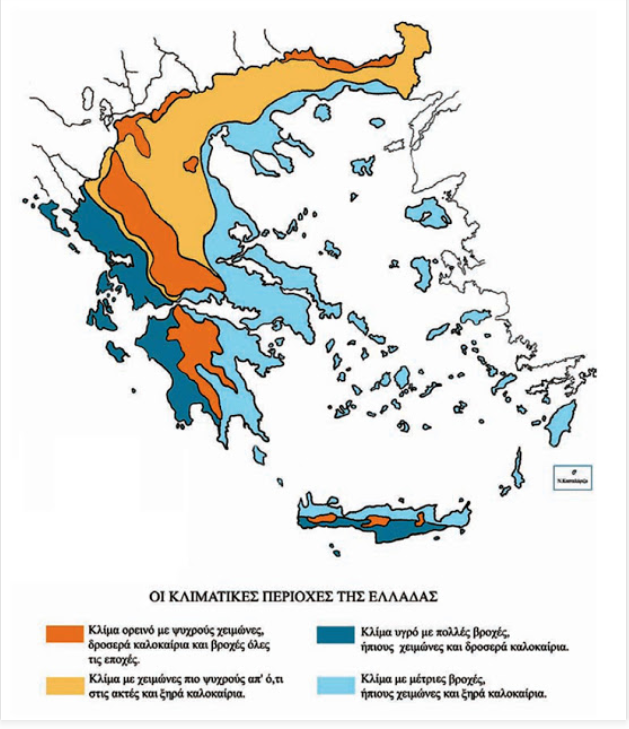
\includegraphics [scale = 0.70] {klima2.png}
			\caption{Κλιματικές περιοχές Ελλάδας}
			\label{klimatikes}
		\end{center}
	\end{figure}
	
	Όπως φαίνεται και στον παραπάνω χάρτη, που απεικονίζει τις κλιματικές περιοχές της Ελλάδας, η πρώτη υποενότητα δεν χαρακτηρίζεται από ενιαίο και ομοιόμορφο κλίμα. Συγκεκριμένα ο νομός Αργολίδας και τα εξωτερικά τμήματα των νομών Κορινθίας και Αρκαδίας χαρακτηρίζονται από κλίμα με μέτριες βροχές με ήπιους χειμώνες και ξηρά καλοκαίρια. Πρόκειται για ένα ημίξηρο κλίμα που συνάδει βεβαίως με το ανάγλυφο της περιοχής, αφού διαθέτει μια μεγάλη ακτογραμμή. Αντίθετα το κεντρικό τμήμα των νομών Αρκαδίας και Κορινθίας έχουν ορεινό κλίμα με ψυχρούς χειμώνες, δροσερά καλοκαίρια και βροχές όλους τους μήνες του έτους. Συνεπώς η πρώτη υποενότητα χωρίζεται σε τρεις κλιματικές ζώνες, τη ζώνη Α, στην οποία ανήκει ο νομός Αργολίδας και το παραθαλάσσιο τμήμα του νομού Αρκαδίας και σύμφωνα με την ενεργειακή ανάλυση των βαθμοημερών θέρμανσης (ΒΗΘ) χαρακτηρίζεται από 601-1100 ΒΗΘ, τη ζώνη Β, στην οποία ανήκει ο νομός Κορινθίας και έχει 1100-1600 ΒΗΘ και τη ζώνη Γ, στην οποία ανήκει ο νομός Αρκαδίας (ορεινή περιοχή) και χαρακτηρίζεται από 1601-2200 ΒΗΘ.
	
	\begin{figure} [H]
		\begin{center}
			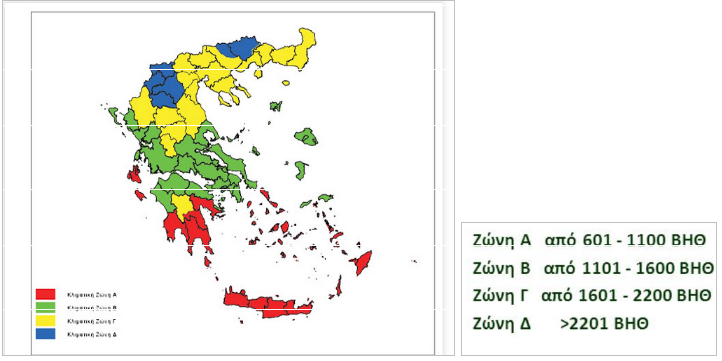
\includegraphics [scale = 0.70] {thermansi.png}
			\caption{Βαθμοημέρες θέρμανσης}
			\label{bathmoimeres}
		\end{center}
	\end{figure}

	\textbf{Θερμοκρασία}
	
	Για την καλύτερη κατανόηση των θερμοκρασιακών στοιχείων της πρώτης υποενότητας, σχεδιάστηκαν διαγράμματα που αφορούν στη μέση μηνιαία θερμοκρασία, στη μέση μέγιστη μηνιαία θερμοκρασία και στη μέση ελάχιστη μηνιαία θερμοκρασία καθενός από τους τρεις νομούς.
	
	Η μέση θερμοκρασία του νομού Αργολίδας κυμαίνεται μεταξύ $8-27°C$ και εμφανίζει μέγιστο στους $34°C$ τον Ιούλιο και ελάχιστο στους $3°C$ τον Ιανουάριο.
	
	\begin{figure} [H]
		\begin{center}
			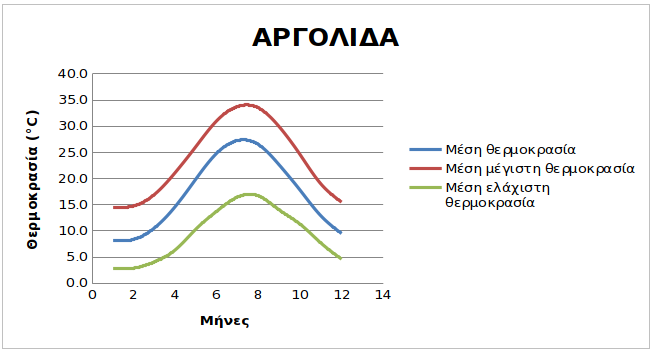
\includegraphics [scale = 0.80] {diagram.png}
		\end{center}
	\end{figure}

	Η μέση θερμοκρασία του νομού Αρκαδίας κυμαίνεται μεταξύ $5-25°C$ και εμφανίζει μέγιστο στους $31°C$ τον Ιούλιο και ελάχιστο στον $1°C$ τον Ιανουάριο.
	
	\begin{figure} [H]
		\begin{center}
			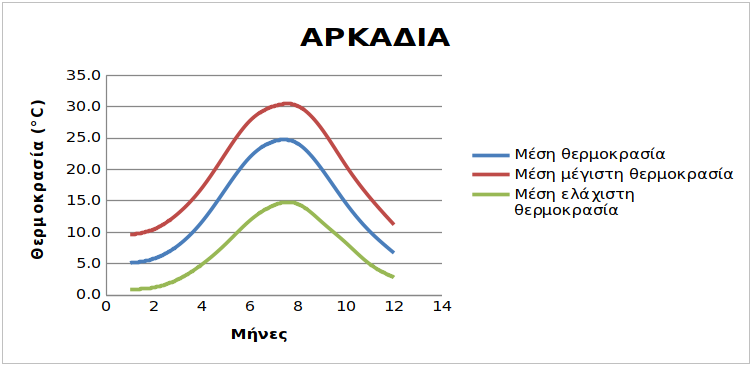
\includegraphics [scale = 0.80] {diagram2.png}
		\end{center}
	\end{figure}

	Η μέση θερμοκρασία του νομού Κορινθίας κυμαίνεται μεταξύ $9-27°C$ και εμφανίζει μέγιστο στους $33°C$ τον Ιούλιο και ελάχιστο στους $5°C$ τον Ιανουάριο.
	
	\begin{figure} [H]
		\begin{center}
			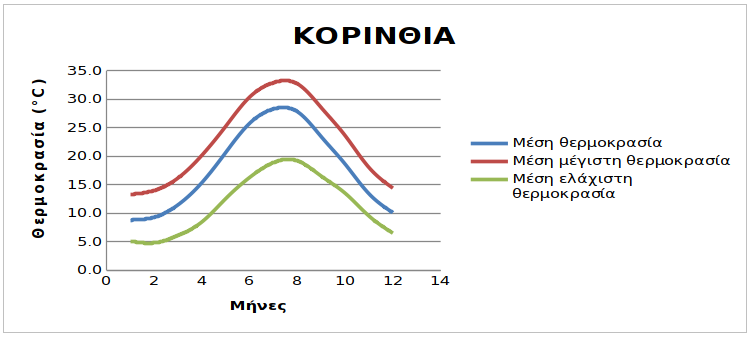
\includegraphics [scale = 0.80] {diagram3.png}
		\end{center}
	\end{figure}

	\textbf{Βροχόπτωση}
	
	Ο κοντινότερος στο νομό Αργολίδας μετεωρολογικός σταθμός της ΕΜΥ που θα μπορούσε να χρησιμοποιηθεί για διεξαγωγή συμπερασμάτων είναι ο σταθμός στο Άστρος. Σύμφωνα λοιπόν με στοιχεία της ΕΜΥ το εύρος του ύψους βροχής του νομού κυμαίνεται περίπου μεταξύ 5-85\eng mm.\gr Τα μέγιστα ύψη εμφανίζονται μεταξύ Νοεμβρίου και Ιανουαρίου ενώ τα ελάχιστα μεταξύ Αυγούστου και Οκτωβρίου. 
	
	\begin{figure} [H]
		\begin{center}
			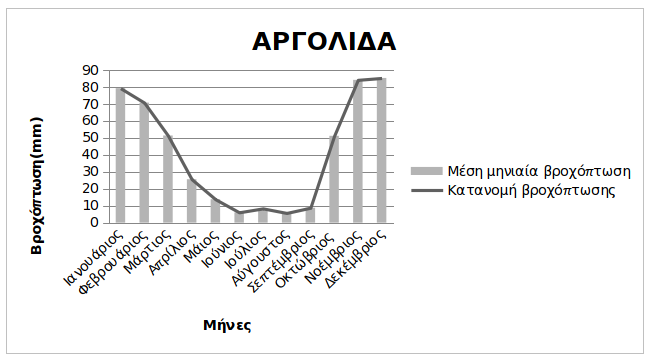
\includegraphics [scale = 0.80] {rain1.png}
		\end{center}
	\end{figure}

	Ο κοντινότερος στο νομό Κορινθίας μετεωρολογικός σταθμός της ΕΜΥ που θα μπορούσε να χρησιμοποιηθεί για διεξαγωγή συμπερασμάτων είναι ο σταθμός στο Βέλο Κορινθίας. Σύμφωνα λοιπόν με στοιχεία της ΕΜΥ το εύρος του ύψους βροχής του νομού κυμαίνεται περίπου μεταξύ 3-88\eng mm. \gr Τα μέγιστα ύψη εμφανίζονται μεταξύ Νοεμβρίου και Ιανουαρίου ενώ τα ελάχιστα μεταξύ Ιουνίου και Σεπτεμβρίου.
	
	\begin{figure} [H]
		\begin{center}
			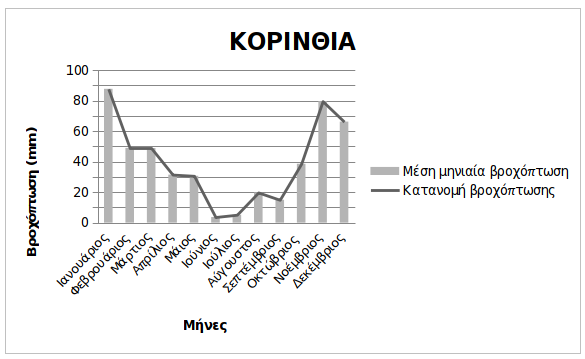
\includegraphics [scale = 0.80] {rain2.png}
		\end{center}
	\end{figure}

	Ο κοντινότερος στο νομό Αρκαδίας μετεωρολογικός σταθμός της ΕΜΥ που θα μπορούσε να χρησιμοποιηθεί για διεξαγωγή συμπερασμάτων είναι ο σταθμός στην Τρίπολη. Σύμφωνα λοιπόν με στοιχεία της ΕΜΥ το εύρος του ύψους βροχής του νομού κυμαίνεται περίπου μεταξύ 20-110mm. Τα μέγιστα ύψη εμφανίζονται μεταξύ Νοεμβρίου και Ιανουαρίου ενώ τα ελάχιστα μεταξύ Ιουνίου και Σεπτεμβρίου.
	
	\begin{figure} [H]
		\begin{center}
			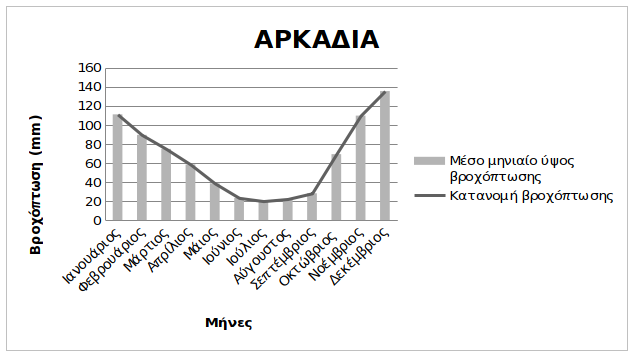
\includegraphics [scale = 0.80] {rain3.png}
		\end{center}
	\end{figure}

	\textbf{Σχετική υγρασία}
	
	Με βάση τα παρακάτω διαγράμματα μέσης  ετήσιας σχετικής υγρασίας, προκύπτουν τα εξής αποτελέσματα για τους τρεις νομούς. Ο Ν. Αργολίδας παρουσιάζει τη μέγιστη μέση σχετική ετήσια υγρασία σε ποσοστό περίπου 77\%, o Ν. Αρκαδίας εμφανίζει τη μέγιστη σχετική υγρασία κατά τους χειμερινούς μήνες και από τους τρεις αυτούς νομούς, σε ποσοστό 78\%, καθώς επίσης και την ελάχιστη σχετική υγρασία κατά τη διάρκεια του καλοκαιριού (45\%). Όλα αυτά, βέβαια, οφείλονται στο διαφορετικό κλίμα που παρουσιάζει η Αρκαδία, ενώ τα ακραία αυτά μεγέθη για τους άλλους νομούς της υποενότητας κυμαίνονται στα ίδια περίπου επίπεδα.
	
	\begin{figure} [H]
		\begin{center}
			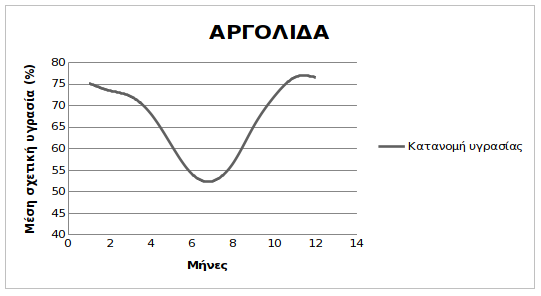
\includegraphics [scale = 0.80] {ygrasia1.png}
		\end{center}
	\end{figure}

	\begin{figure} [H]
		\begin{center}
			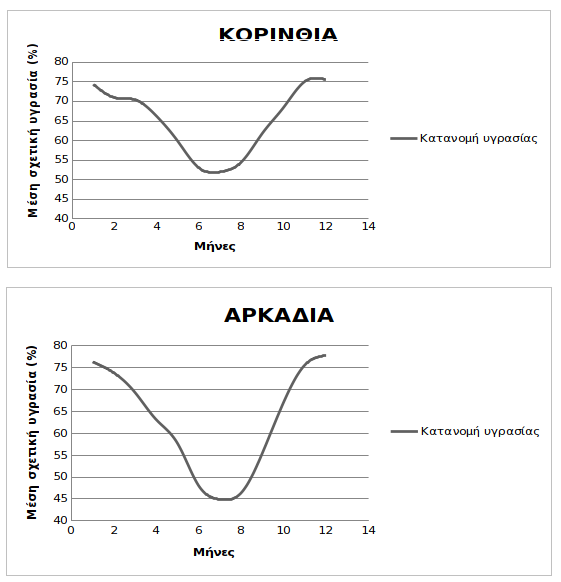
\includegraphics [scale = 0.80] {ygrasia2.png}
		\end{center}
	\end{figure}

	\textbf{Ένταση ανέμου}
	
	Η μέση ετήσια  ένταση του ανέμου για την πρώτη υποενότητα παρουσιάζεται στα παρακάτω διαγράμματα.
	
	\begin{figure} [H]
		\begin{center}
			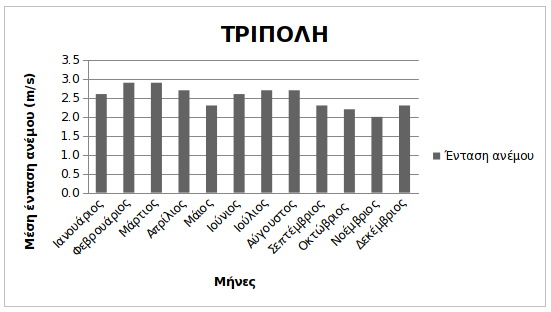
\includegraphics [scale = 0.80] {wind1.png}
		\end{center}
	\end{figure}
	
	\begin{figure} [H]
		\begin{center}
			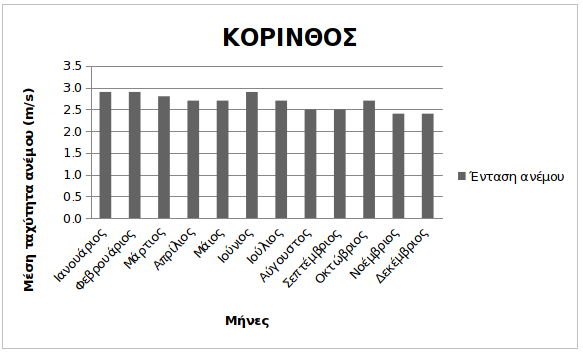
\includegraphics [scale = 0.80] {wind2.png}
		\end{center}
	\end{figure}

	\begin{figure} [H]
		\begin{center}
			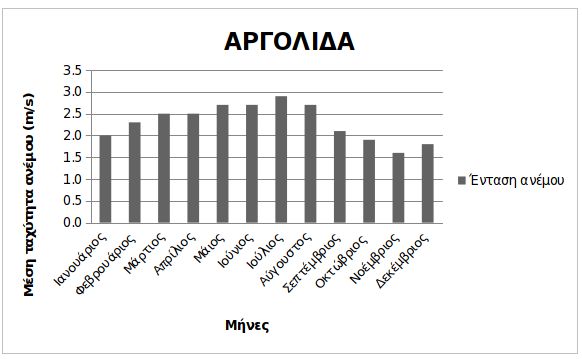
\includegraphics [scale = 0.80] {wind3.png}
		\end{center}
	\end{figure}

	\subsubsection{Ανθρωπογενές Περιβάλλον}
	
	\paragraph{Πληθυσμιακά στοιχεία}
	
	Με βάση την τελευταία απογραφή πληθυσμού που πραγματοποιήθηκε το 2011 από την Ελληνική Στατιστική Αρχή (ΕΛ.ΣΤΑ.Τ.) προκύπτουν τα εξής συμπεράσματα για την πρώτη υποενότητα της περιφέρειας Πελοποννήσου. Αρχικά, πρόκειται για την μεγαλύτερη πληθυσμιακά υποενότητα με ποσοστό 56,90\% επί του συνολικού (577.903 κάτοικοι). Το μεγαλύτερο τμήμα της ανήκει στην περιφερειακή ενότητα Κορινθίας, μιας και φτάνει το 44,12\% του αριθμού των κατοίκων της υποενότητας αυτής (328.811 κάτοικοι). Αμέσως μετά ακολουθεί η Π.Ε. Αργολίδας (29,51\%) και τέλος η Π.Ε. Αρκαδίας (26,36\%), λαμβάνοντας υπόψη, ωστόσο μόνο τα πληθυσμιακά μεγέθη των δήμων της που υπάγονται στην πρώτη υποενότητα. Πιο αναλυτικά τα στοιχεία δίνονται στους παρακάτω πίνακες:  
	
	\begin{table}[H]
		\centering
		\begin{tabular}{|c|c|}
			\hline
			\textbf{ΑΡΓΟΛΙΔΑ} & \textbf{ΠΛΗΘΥΣΜΟΣ} \\ \hline
			ΔΗΜΟΣ ΝΑΥΠΛΙΕΩΝ & 33.356 \\ \hline
			ΔΗΜΟΣ ΑΡΓΟΥΣ-ΜΥΚΗΝΩΝ & 42.022 \\ \hline
			ΔΗΜΟΣ ΕΠΙΔΑΥΡΟΥ & 8.115 \\ \hline
			ΔΗΜΟΣ ΕΡΜΙΟΝΙΔΑΣ & 13.551 \\ \hline
			ΠΛΗΘΥΣΜΟΣ Ν. ΑΡΓΟΛΙΔΑΣ & 97.044 \\ \hline
		\end{tabular}
		\caption{Πληθυσμός Περιφερειακής Ενότητας Αργολίδας}
		\label{The label}
	\end{table}

	\begin{table}[H]
		\centering
		\begin{tabular}{|c|c|}
			\hline
			\textbf{ΑΡΚΑΔΙΑ} & \textbf{ΠΛΗΘΥΣΜΟΣ} \\ \hline
			ΔΗΜΟΣ ΤΡΙΠΟΛΗΣ & 47.254 \\ \hline
			ΔΗΜΟΣ ΒΟΡΕΙΑΣ ΚΥΝΟΥΡΙΑΣ & 10.341 \\ \hline
			ΔΗΜΟΣ ΝΟΤΙΑΣ ΚΥΝΟΥΡΙΑΣ & 8.294 \\ \hline
			ΠΛΗΘΥΣΜΟΣ Ν. ΑΡΚΑΔΙΑΣ & 86.685 \\ \hline
		\end{tabular}
		\caption{Πληθυσμός Περιφερειακής Ενότητας Αρκαδίας}
		\label{The label}
	\end{table}

	\begin{table}[H]
		\centering
		\begin{tabular}{|c|c|}
			\hline
			\textbf{ΚΟΡΙΝΘΙΑ} & \textbf{ΠΛΗΘΥΣΜΟΣ} \\ \hline
			ΔΗΜΟΣ ΚΟΡΙΝΘΙΩΝ & 58.192 \\ \hline
			ΔΗΜΟΣ ΒΕΛΟΥ-ΒΟΧΑΣ & 19.027 \\ \hline
			ΔΗΜΟΣ ΛΟΥΤΡΑΚΙΟΥ-ΑΓΙΩΝ & \\
			ΘΕΟΔΩΡΩΝ-ΠΕΡΑΧΩΡΑΣ & 21.221 \\ \hline
			ΔΗΜΟΣ ΝΕΜΕΑΣ & 6.483 \\ \hline
			ΔΗΜΟΣ ΞΥΛΟΚΑΣΤΡΟΥ-ΕΥΡΩΣΤΙΝΗΣ & 17.365 \\ \hline
			ΔΗΜΟΣ ΣΙΚΥΩΝΙΩΝ & 22.794 \\ \hline
			ΠΛΗΘΥΣΜΟΣ Ν. ΚΟΡΙΝΘΙΑΣ & 145.082 \\ \hline
		\end{tabular}
		\caption{Πληθυσμός Περιφερειακής Ενότητας Κορινθίας}
		\label{The label}
	\end{table}
	
	\paragraph{Χρήσεις γης}
	
	\begin{figure} [H]
		\begin{center}
			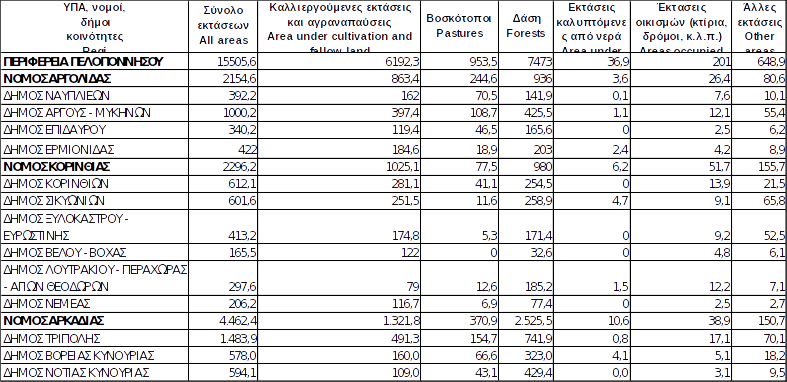
\includegraphics [scale = 0.80] {xriseis2.png}
			\caption{Χρήσεις γης}
		\end{center}
	\end{figure}

	\paragraph{Πολιτιστική Κληρονομιά}
	
	\textbf{Περιοχές αρχαιολογικού και ιστορικού ενδιαφέροντος}
	
	Οι νομοί της πρώτης υποενότητας διαθέτουν σπουδαία αρχαία και σύχρονη ιστορία. Αποτελούν ένα από το σημαντικότερα κομμάτια του ελληνικής αλλά και της ευρωπαϊκής κληρονομιάς. Συγκεκριμένα, στο Ν. Αργολίδας εντοπίζεται ένας από τους τρεις αρχαιότερους πολιτισμούς του ελλαδικού χώρου, ο Μυκηναϊκός, καθώς και το αξιοσημείωτο θέατρο της Επιδαύρου. Επιπλέον, στο υψηλότερο τμήμα της Ακροναυπλίας τοποθετείται το κάστρο Παλαμίδι μεγάλης στρατηγικής σημασίας, καθώς και το περιβαλλόμενο από θάλασσα κάστρο Μπούρτζι που βρίσκεται ακριβώς απέναντι της πόλης του Ναυπλίου. 
	
	Η Κορινθία και συγκεκριμένα η Αρχαία πόλη της Κορίνθου αποτελούσε σημαντική πόλη-κράτος της αρχαίας Πελοποννήσου. Στοιχεία που μαρτυρούν την ύπαρξή της αποτελούν οι αρχαιολογικοί χώροι που βρίσκονται διάσπαρτοι σε όλη σχεδόν την έκτασή της. Τέτοιοι είναι ο αρχαϊκός ναός του Απόλλωνα, η Ακροκόρινθος και πολλά άλλα που καταγράφονται στον επόμενο πίνακα.
	
	Ο Ν. Αρκαδίας πρωταγωνίστησε στους αγώνες του Έθνους για την ελευθερία, παίζοντας σημαντικό ρόλο εξέλιξη της πιο σύγχρονης ιστορίας. Ωστόσο πολλά από τα μνημεία της είναι επηρεασμένα από την μυθολογία, γεγονός το οποίο μαρτυρά την παλαιότητα της Αρκαδίας και συνάμα την σπουδαιότητά της. 
	
	\underline{Νομός Αργολίδας}
	
	\begin{table}[H]
		\centering
		\begin{tabular}{|c|c|}
			\hline
			\multicolumn{2}{|c|}{\textbf{ΑΡΧΑΙΟΛΟΓΙΚΟΙ ΧΩΡΟΙ ΚΑΙ ΜΝΗΜΕΙΑ}} \\ \hline
			ΑΚΡΟΠΟΛΗ ΑΛΙΕΩΝ & ΜΝΗΜΕΙΑ ΕΡΜΙΟΝΙΔΑΣ \\ \hline
			ΣΠΗΛΑΙΟ ΦΡΑΓΧΘΙ ΕΡΜΙΟΝΙΔΑΣ & ΑΚΡΟΠΟΛΗ ΚΑΖΑΡΜΑΣ \\ \hline
			ΑΡΧΑΙΑ ΑΣΙΝΗ & ΠΡΩΗΝ ΣΤΡΑΤΙΩΤΙΚΗ \\ & ΣΧΟΛΗ ΕΥΕΛΠΙΔΩΝ \\ \hline
			ΜΥΚΗΝΑΙΚΗ ΓΕΦΥΡΑ ΚΑΖΑΡΜΑΣ & ΚΑΣΤΡΟ ΠΑΛΑΜΗΔΙΟΥ \\ \hline
			ΜΠΟΥΡΤΖΙ & ΑΡΧΑΙΑ ΤΙΡΥΝΘΑ \\ \hline
			ΠΑΛΑΙΑ ΠΟΛΗ ΝΑΥΠΛΙΟΥ & ΕΛΛΗΝΙΣΤΙΚΗ ΠΥΡΑΜΙΔΑ \\ & ΕΛΛΗΝΙΚΟΥ \\ \hline
			ΛΕΡΝΑ & ΚΑΣΤΡΟ ΛΑΡΙΣΑ ΚΑΙ \\ & ΜΝΗΜΕΙΑ ΤΟΥ ΑΡΓΟΥΣ \\ \hline
			ΜΟΝΗ ΑΡΕΙΑΣ & ΙΕΡΑ ΑΠΟΛΛΩΝΟΣ ΔΕΙΡΑΔΙΩΤΗ \\ \hline
			ΑΡΧΑΙΑ ΑΓΟΡΑ ΑΡΓΟΥΣ & ΔΗΜΟΤΙΚΗ ΑΓΟΡΑ ΑΡΓΟΥΣ \\ \hline
			ΗΡΑΙΟΝ ΑΡΓΟΥΣ & ΝΑΟΣ ΚΟΙΜΗΣΗΣ \\ & ΘΕΟΤΟΚΟΥ ΜΕΡΜΠΑΚΑ \\ \hline
			ΑΡΧΑΙΟ ΘΕΑΤΡΟ ΑΡΓΟΥΣ & ΝΑΟΣ ΚΟΙΜΗΣΗΣ \\ & ΘΕΟΤΟΚΟΥ ΧΩΝΙΚΑ \\ \hline
			ΜΙΔΕΑ & ΚΑΣΤΡΟ ΛΑΡΙΣΑ ΚΑΙ \\ & ΜΝΗΜΕΙΑ ΤΟΥ ΑΡΓΟΥΣ \\ \hline
			ΜΟΝΗ ΑΡΕΙΑΣ & ΤΑΦΙΚΟΣ ΚΥΚΛΟΣ Β' \\ \hline
			ΥΠΟΓΕΙΑ ΔΕΞΑΜΕΝΗ & ΠΥΛΗ ΛΕΟΝΤΩΝ \\ \hline
			ΣΥΝΟΙΚΙΑ ΛΑΔΕΜΠΟΡΟΥ & ΘΡΗΣΚΕΥΤΙΚΟ ΚΕΝΤΡΟ ΜΥΚΗΝΩΝ \\ \hline
			ΚΥΚΛΩΠΕΙΑ ΤΕΙΧΗ & ΘΟΛΩΤΟΣ ΤΑΦΟΣ ΤΟΥ ΑΤΡΕΩΣ \\ \hline
			ΑΣΚΛΗΠΙΕΙΟ ΕΠΙΔΑΥΡΟΥ & ΑΡΧΑΙΟ ΘΕΑΤΡΟ \\ & ΑΣΚΛΗΠΙΕΙΟΥ ΕΠΙΔΑΥΡΟΥ \\ \hline
			ΘΕΑΤΡΟ ΑΡΧΑΙΑΣ ΠΟΛΕΩΣ ΕΠΙΔΑΥΡΟΥ & ΜΝΗΜΕΙΑ ΛΙΓΟΥΡΙΟΥ \\ \hline
		\end{tabular}
		\caption{Αρχαιολογικοί χώροι Αργολίδας}
		\label{The label}
	\end{table}
	
	\begin{table}[H]
		\centering
		\begin{tabular}{|c|c|}
			\hline
			\multicolumn{2}{|c|}{\textbf{ΑΡΧΑΙΟΛΟΓΙΚΟΙ ΧΩΡΟΙ ΚΑΙ ΜΝΗΜΕΙΑ}} \\ \hline
			ΑΡΧΑΙΑ ΔΙΟΛΚΟΣ & ΙΕΡΟ ΤΟΥ ΠΟΣΕΙΔΩΝΑ \\ & ΣΤΗΝ ΙΣΘΜΙΑ \\ \hline
			ΑΡΧΑΙΑ ΚΟΡΙΝΘΟΣ & ΑΚΡΟΚΟΡΙΝΘΟΣ \\ \hline
			ΠΑΛΑΙΟΧΡΙΣΤΙΑΝΙΚΗ & \\ ΒΑΣΙΛΙΚΗ ΛΕΧΑΙΟΥ & ΘΕΑΤΡΟ ΣΙΚΥΩΝΟΣ \\ \hline
			ΑΡΧΑΙΟΛΟΓΙΚΟΣ ΧΩΡΟΣ ΣΙΚΥΩΝΟΣ & ΣΤΥΜΦΑΛΟΣ \\ \hline
			ΜΟΝΗ ΑΓΙΟΥ ΓΕΩΡΓΙΟΥ & ΠΕΡΑΧΩΡΑ \\ \hline
			ΙΕΡΟ ΤΟΥ ΔΙΟΣ ΣΤΗ ΝΕΜΕΑ & ΣΤΑΔΙΟ ΝΕΜΕΑΣ \\ \hline
		\end{tabular}
		\caption{Αρχαιολογικοί χώροι Κορινθίας}
		\label{The label}
	\end{table}
	
	\begin{table}[H]
		\centering
		\begin{tabular}{|c|c|}
			\hline
			\multicolumn{2}{|c|}{\textbf{ΑΡΧΑΙΟΛΟΓΙΚΟΙ ΧΩΡΟΙ ΚΑΙ ΜΝΗΜΕΙΑ}} \\ \hline
			ΟΡΧΟΜΕΝΟΣ ΑΡΚΑΔΙΑΣ & ΤΕΙΧΟΣ ΜΑΝΤΙΝΕΙΑΣ \\ \hline
			ΝΑΟΣ ΤΗΣ ΗΡΑΣ & ΑΡΧΑΙΟΣ ΝΑΟΣ ΣΤΟ \\ & ΓΚΟΡΓΚΟΣΟΥΛΙ \\ \hline
			ΑΡΧΑΙΟ ΘΕΑΤΡΟ ΜΑΝΤΙΝΕΙΑΣ & ΙΕΡΟ ΙΠΠΙΟΥ ΠΟΣΕΙΔΩΝΑ \\ \hline
			ΜΑΛΛΙΑΡΟΠΟΥΛΕΙΟ ΔΗΜΟΤΙΚΟ ΘΕΑΤΡΟ & ΝΑΟΣ ΤΗΣ ΑΛΕΑΣ ΑΘΗΝΑΣ \\ \hline
			ΜΝΗΜΕΙΑ ΤΗΣ ΤΕΓΕΑΣ & ΜΟΝΗ ΤΗΣ ΜΑΛΕΒΗΣ \\ \hline
			ΜΟΝΗ ΜΕΤΑΜΟΡΦΩΣΗΣ & \\ΣΩΤΗΡΟΣ ΛΟΥΚΩΣ & ΡΩΜΑΙΚΗ ΕΠΑΥΛΗ \\ & ΤΟΥ ΛΟΥΚΟΥ ΚΥΝΟΥΡΙΑΣ \\ \hline
			ΚΑΣΤΡΟ ΠΑΡΑΑΙΟΥ ΑΣΤΡΟΥΣ & ΜΝΗΜΕΙΑ ΤΟΥ ΠΡΑΣΤΟΥ \\ \hline
			ΜΟΝΗ ΚΑΛΤΕΖΩΝ & ΜΟΝΗ ΜΠΟΥΡΑ ΦΑΛΑΣΙΑΣ \\ \hline
			ΜΝΗΜΕΙΑ ΤΟΥ ΛΕΟΝΤΑΡΙΟΥ & ΜΕΓΑΛΟΠΟΛΗ \\ \hline
			ΙΕΡΟ ΤΗΣ ΔΕΣΠΟΙΝΑΣ & \\ - ΛΥΚΟΣΟΥΡΑ & ΙΕΡΟ ΛΥΚΑΙΟΥ ΔΙΟΣ \\ \hline
			ΚΑΣΤΡΟ ΤΗΣ ΚΑΡΥΤΑΙΝΑΣ ΚΑΙ & \\ ΝΑΟΙ ΤΟΥ ΟΙΚΙΣΜΟΥ & ΜΝΗΜΕΙΑ ΤΗΣ ΣΤΕΜΝΙΤΣΑΣ \\ \hline
		\end{tabular}
		\caption{Αρχαιολογικοί χώροι Αρκαδίας}
		\label{The label}
	\end{table}
	
	\subsection{2η  Υποενότητα}
	
	\subsubsection{Φυσικό Περιβάλλον}
	
	\paragraph{Ανάγλυφο}
	
	\textbf{Γεωγραφία}
	
	Η δεύτερη υποενότητα αποτελείται από το νομό Μεσσηνίας και τμήμα του νομού Αρκαδίας. Ο νομός Μεσσηνίας  βρίσκεται στο νοτιοδυτικό άκρο της Πελοποννήσου έχει έκταση 2995 τ.χλμ., 159.954 κατοίκους (Απογραφή 2011) και πρωτεύουσα την Καλαμάτα. Στα βόρεια συνορεύει με  το νομό Ηλείας, στα βόρεια και βορειοανατολικά με το νομό Αρκαδίας και στα Ανατολικά με το νομό Λακωνίας. Διαθέτει συνολικά έξι δήμους, οι οποίοι είναι οι εξής:
	
	\begin{table}[H]
		\centering
		\begin{tabular}{|c|c|}
			\hline
			\textbf{Α/Α} & \textbf{Δήμος} \\ \hline
			1 & Δυτικής Μάνης \\ \hline
			2 & Καλαμάτας \\ \hline
			3 & Μεσσήνης \\ \hline
			4 & Οιχαλίας \\ \hline
			5 & Πύλου-Νέστορος \\ \hline
			6 & Τριφυλίας \\ \hline
		\end{tabular}
		\caption{Δήμοι Νομού Μεσσηνίας}
		\label{The label}
	\end{table}
	
	Ο νομός Αρκαδίας καταλαμβάνει το κέντρο της Πελοποννήσου. Συνορεύει βόρεια με τους νομούς Κορινθίας και Αχαΐας, δυτικά με τους νομούς Ηλείας και Μεσσηνίας, νότια με το νομό Λακωνίας και ανατολικά βρέχεται από τον Αργολικό κόλπο. Έχει έκταση 4.419 τετραγωνικά χιλιόμετρα και πληθυσμό 102.035 \footnote{Σύμφωνα με τα αποτελέσματα της απογραφής του 2001} κατοίκους. Πρωτεύουσα του νομού είναι η Τρίπολη και σημαντικές κωμοπόλεις το 'Αστρος, η Βυτίνα, η Δημητσάνα, τα Λαγκάδια, το Λεβίδι, το Λεωνίδιο, η Μεγαλόπολη, τα Τρόπαια. Ο νομός διαθέτει συνολικά πέντε δήμους, οι οποίοι είναι οι εξής:
	
	\begin{table} [H]
		\centering
		\begin{tabular}{|c|c|}
			\hline
			\textbf{Α/Α} & \textbf{Δήμος} \\ \hline
			1 & Γορτυνίας \\ \hline
			2 & Λεωνιδίου \\ \hline
			3 & Τρίπολης \\ \hline
			4 & Μεγαλόπολης \\ \hline
			5 & Βόρειας Κυνουρίας \\ \hline
		\end{tabular}
		\caption{Δήμοι Νομού Αρκαδίας}
		\label{The label}
	\end{table}
	
	Οι δήμοι που ανήκουν στην δεύτερη υποενότητα είναι οι δήμοι Γορτυνίας και Μεγαλόπολης στα δυτικά του νομού στα σύνορα με τη Μεσσηνία.Όπως φαίνεται στον γεωμορφολογικό χάρτη (βλ. σελιδα \pageref{peloponnese}) η Μεσσηνία έχει κατά βάση πεδινή έκταση με εξαίρεση κάποιες οροσειρές σε ορισμένα σημεία της, ενώ αντίθετα η Αρκαδία είναι στο σύνολό της ορεινή.
	
	Συγκεκριμένα στο νομό Μεσσηνίας το ψηλότερο βουνό είναι ο Ταΰγετος (2404 μ., κορυφή Προφήτης Ηλίας), τον οποίο η Μεσσηνία μοιράζεται με τη Λακωνία και εκτείνεται σε μήκος 115χλμ και του οποίου η οροσειρά συνεχίζεται με άλλες ψηλές κορυφές προς βορειοδυτικά. Στα βορειοανατολικά σύνορα με την Αρκαδία και σε μικρή απόσταση από την Ανδρίτσαινα της Ηλείας βρίσκεται το Λύκαιο (1420 μ.). Στα βόρεια σύνορα με την Ηλεία βρίσκεται το Τετράζιο. Στα δυτικά και προς το Ιόνιο Πέλαγος εκτείνονται από βορρά προς νότο τα όρη της Κυπαρισσίας (όρος Αιγάλεω, 1224 μ), στην προέκταση των οποίων βρίσκεται, στη δυτική μεσσηνιακή χερσόνησο, το όρος Λυκόδημος (960 μ.). 
	
	Στο κέντρο του νομού και από βορρά προς νότο εκτείνεται η ευφορότατη πεδιάδα της Μεσσηνίας. Η μεγαλύτερη έκταση είναι η λεκάνη απορροής του ποταμού Πάμισου που αποτελείται βόρεια από την πεδιάδα του Μελιγαλά, και νότια από την ευρύτερη πεδιάδα της Καλαμάτας που φτάνει στα παράλια του Μεσσηνιακού Κόλπου. Επίσης υπάρχουν και άλλες μικρότερες πεδιάδες όπως της Κυπαρισσίας, των Γαργαλιάνων, της Πύλου, της Μεθώνης, της Κορώνης, του Λογγά και του Πεταλιδίου.
	
	Μεγαλύτερο ποτάμι είναι ο Πάμισος, ο οποίος διασχίζει την πεδιάδα της Καλαμάτας και εκβάλλει στο Μεσσηνιακό Κόλπο. Στα σύνορα με την Ηλεία βρίσκεται ο ποταμός Νέδα. Μικρότερα ποτάμια είναι ο Βελίκας και ο Νέδωνας, που διασχίζουν την πόλη της Καλαμάτας. 
	
	Στο νομό Αρκαδίας στους δήμους της δεύτερης υποενότητας ανήκει εν μέρει ο ψηλότερος ορεινός όγκος της Αρκαδίας, το όρος Μαίναλο (1981μ.) καθώς και πολύ μικρό τμήμα της οροσειράς του Ταΰγετου.
	
	Όπως ειπώθηκε παραπάνω το τμήμα του νομού Αρκαδίας που ανήκει στη δεύτερη υποενότητα είναι κατά κύριο λόγο ορεινό με εξαίρεση το λεκανοπέδιο της Μεγαλόπολης στα σύνορα του νομού με τη Μεσσηνία.
	
	Ο σημαντικότερος ποταμός είναι ο Αλφειός που πηγάζει από τα οροπέδια της Μεγαλόπολης και ο Λάδωνας που πηγάζει από καρστικές πηγές στα βόρεια του νομού.
	
	Μοναδική λίμνη στην περιοχή αυτή είναι η τεχνητή λίμνη του Λάδωνα στα σύνορα με το νομό Αχαΐας.   
	
	\textbf{Ακτογραφία}
	
	Ο νομός Μεσσηνίας, καθότι βρίσκεται στο νοτιοδυτικό άκρο της Πελοποννήσου, διαβρέχεται από θάλασσα στα νότια και τα δυτικά (βλ. σελιδα \pageref{peloponnese}). Αναλυτικά στα δυτικά και νοτιοδυτικά βρέχεται από το Ιόνιο Πέλαγος, ενώ στα νότια από τη Μεσόγειο Θάλασσα. Η δυτική ακτογραμμή ξεκινά από το νότιο τμήμα του Κυπαρισσιακού Κόλπου στις εκβολές του ποταμού Νέδα και συνεχίζοντας νότια συναντά το στενό της Πρώτης που βρίσκεται ανάμεσα στο νησί Πρώτη και το ηπειρωτικό τμήμα του νομού και ύστερα τη λιμνοθάλασσα Ντιβάρι και τον Όρμο Ναυαρίνου που βρίσκεται ανάμεσα στο νησί Σφακτηρία και την ηπειρωτική Μεσσηνία. Στη συνέχεια πλησιάζοντας προς το νοτιότερο τμήμα του νομού συναντά τον Όρμο της Μεθώνης, όπου και ξεκινά η στροφή της ακτογραμμής προς τα ανατολικά με εντονότερες ανωμαλίες και αλλεπάλληλες διεισδύσεις προς τη θάλασσα και υποχωρήσεις προς την ξηρά. Το στενό της Μεθώνης διαχωρίζει τις ακτές της Μεσσηνίας από τα νησιά Σαπιέντζα, Μπόμπα, Κουλουρά, Δυο Αδέρφια και Αγ. Μαρίνα. Δίπλα στα νησιά αυτά βρίσκεται και το νησί Σχίζα. Στη συνέχεια η ακτογραμμή συνεχίζει προς τα νότια και καταλήγει στο νοτιότερο σημείο του νομού στο ακρωτήριο Ακρίτας. Το στενό στο σημείο αυτό περνά ανάμεσα στο νησί Βενέδικτο και τις νότιες ακτές της Μεσσηνίας και σηματοδοτεί την έναρξη του Μεσσηνιακού Κόλπου. Στην περιοχή αυτή η ακτογραμμή ξεκινά την κίνηση της σταδιακά προς τα βόρεια και ύστερα από τη χερσόνησο της Κορώνης φτάνει στον όρμο του Πεταλιδίου χωρίς ιδιαίτερες ανωμαλίες. Ύστερα η ακτογραμμή της Μεσσηνίας κατευθύνεται προς τα ανατολικά και αφού συναντήσει τις εκβολές του ρέματος Βελίκα σχηματίζει την παραλία της Καλαμάτας και καταλήγει στο λιμάνι της πόλης. Από εκεί συνεχίζει προς τα νότια και πριν τερματίσει βόρεια του Όρμου Λιμενίου του νομού Λακωνίας συναντά τον Όρμο και το ακρωτήρι Κιτριών.   
	
	Το τμήμα του νομού Αρκαδίας που ανήκει στη δεύτερη υποενότητα (Δήμος Γορτυνίας και Δήμος Μεγαλόπολης) βρίσκεται περίπου στο κέντρο της Πελοποννήσου και δεν επικοινωνεί με θάλασσα.
	
	\paragraph{Έδαφος-Γεωλογία-Υδατικοί πόροι}
	
	\textbf{Έδαφος}
	
	Σύμφωνα με την ταξινόμηση των εδαφών (βλ. σελίδα \pageref{edafi}), βάσει του συστήματος FAO (Χάρτης Εδαφών Ελλάδας – Εθνική Επιτροπή κατά της Ερημοποίησης – Γεωπονικό Πανεπιστήμιο Αθηνών – Συντάκτης Ν. Γιάσογλου – ( Παράρτημα IΙ ), τα εδάφη της δεύτερης υποενότητας ταξινομούνται σε έξι κατηγορίες εδαφών, οι οποίες είναι:
	
	\begin{itemize}
		\item \emph{Βράχοι}(Rock Outcrops) (μαύρο χρώμα)
		\item \emph{\selectlanguage{english}Leptosols}\selectlanguage{english}(LP): \selectlanguage{greek}Εδάφη με μητρικό υλικό από ασβεστόλιθο και φλύσχη. Είναι λεπτόκοκκα εδάφη, αργιλώδη, καλής υδατοπερατότητας με ουδέτερο \selectlanguage{english}pH. \selectlanguage{greek}(γκρι χρώμα)
		\item \emph{\selectlanguage{english}Regosols}\selectlanguage{english}(RG): \selectlanguage{greek}Στρώμα χαλαρού υλικού, πάνω σε σκληρό υπόβαθρο. Είναι εδάφη μετρίως αργιλώδη, με μέτρια υδατοπερατότητα και με \selectlanguage{english}pH $>$ 7.\selectlanguage{greek}(κίτρινο χρώμα)
		\item \emph{\selectlanguage{english}Fluvisols}\selectlanguage{english}(FL): \selectlanguage{greek}Εδάφη αργιλώδη, με μέτρια έως μικρή υδατοπερατότητα και με \selectlanguage{english}pH $>$ 7.\selectlanguage{greek}(μπλε χρώμα)
		\item \emph{\selectlanguage{english}Cambisols}\selectlanguage{english}(CM): \selectlanguage{greek}Η σύσταση των εδαφών αυτών είναι αργιλλώδης και μετρίως αργιλλώδης, με μικρή υδατοπερατότητα και με ουδέτερο ή ελαφρώς όξινο \selectlanguage{english}pH. \selectlanguage{greek}(πορτοκαλί χρώμα)
		\item \emph{\selectlanguage{english}Luvisols}\selectlanguage{english}(LV): \selectlanguage{greek}Τα εδάφη αυτά είναι αργιλώδη με υψηλή υδατοπερατότητα και με \selectlanguage{english}pH $\approx$ 7.\selectlanguage{greek}(ροζ χρώμα)
	\end{itemize}

	Η παραπάνω ανάλυση των εδαφών είναι από το βιβλίο Μαθήματα Εφαρμοσμένης Εδαφολογίας του Νικολάου Ιωάν Γιάσογλου (Αθήνα  Ιανουάριος 1995)
	
	Συμπερασματικά λοιπόν και σύμφωνα με τα παραπάνω στοιχεία το έδαφος της  είναι αργιλλοαμώδες με ουδέτερο προς αλκαλικό \eng pH,\gr πολύ εύφορο στα πεδινά έως πετρώδες μικρής γονιμότητας στα ορεινά. Τα εδάφη της Μεσσηνίας είναι μετρίως υδατοπερατά με ικανοποιητική στράγγιση και ευχέρεια μετακίνησης νερού και εδαφικών διαλυμάτων, με αποτέλεσμα να μην κρατούν νερό και να μην δημιουργούν ρωγμές στο έδαφος. Επίσης έχουν κάποια περιεκτικότητα σε φώσφορο, ενώ σε άζωτο ή κάλιο παρουσιάζουν κάποια έλλειψη. Το μεγαλύτερο μέρος των εδαφών είναι λοφώδες και από μηχανικής απόψεως κατατάσσονται στα ελαφρά έως μέσης συστάσεως.
	
	Το έδαφος του τμήματος του νομού Αρκαδίας που ανήκει στη δεύτερη υποενότητα είναι κατά βάση αργιλώδες με υψηλή υδατοπερατότητα με εξαίρεση τη βραχώδη ζώνη στα βόρεια του νομού και ένα τμήμα μετρίως αργιλλώδες με μικρή υδατοπερατότητα στην περιοχή της Μεγαλόπολης.
	
	Όπως φαίνεται στο χάρτη δυνητικού κινδύνου ερημοποίησης της Ελλάδας (βλ. σελίδα \pageref{erimopoiisi})που συνετάχθη από την Εθνική Επιτροπή κατά της Ερημοποίησης το έδαφος της δεύτερης υποενότητας κατατάσσεται ως μετρίου κινδύνου στην περιοχή της Μεσσηνίας και υψηλού κινδύνου στην περιοχή της Αρκαδίας.
	
	\textbf{Γεωλογία-Τεκτονική: Γεωτεκτονικές ζώνες Δεύτερης Υποενότητας}
	
	Οι γεωτεκτονικές ζώνες που εμφανίζονται στη δεύτερη υποενότητα (βλ. σελίδα 9\pageref{geotektonikes}) είναι οι εξής:
	
	\begin{enumerate}
		\item \textbf{Ζώνη Ολωνού-Πίνδου} \\
		Κατέχει κεντρική θέση στον κορμό της Ελλάδας και ακολουθεί την κάμψη του ορογενετικού τόξου, ενώ τμήματα της απαντούν στην Κρήτη και τη Ρόδο. Συνίσταται από ασβεστόλιθους, δολομίτες, κερατόλιθους, ηφαιστειοϊζηματογενή πετρώματα, ραδιολαρίτες, αργίλους, ψαμμίτες και πηλίτες. Έχει επωθηθεί προς τα δυτικά πάνω στη ζώνη Γαβρόβου-Τριπόλεως και χαρακτηρίζεται από δομή λεπίων, με αποτέλεσμα συχνές επαναλήψεις των στρωμάτων. Πάνω στη ζώνη της Πίνδου βρίσκονται επωθημένες οι μεγαλύτερες οφιολιθικές μάζες του ελληνικού χώρου.
		\item \textbf{Ζώνη Γαβρόβου-Τριπόλεως} \\
		Η ζώνη Γαβρόβου - Τριπόλεως χαρακτηρίζεται από συνεχή ανθρακική ιζηματογένεση με κυρίαρχα πετρώματα τους ασβεστόλιθους και δολομίτες. Οι σχηματισμοί της ζώνης αυτής επικάθονται σε ένα υπόβαθρο αποτελούμενο από φυλλίτες, χαλαζιακούς φυλλίτες και μάρμαρα, γνωστό ως «φυλλιτική-χαλαζιτική» σειρά. Τα στρώματά της σχηματίζουν μεγάλα ανοικτά σύγκλινα και αντίκλινα και είναι επωθημένη δυτικά πάνω στην Ιόνιο ζώνη.
		\item \textbf{Ζώνη Παξών (ή Προαπούλια)} \\
		Είναι η  πιο εξωτερική γεωτεκτονική ζώνη της Ελλάδας, της οποίας εμφανίζεται  ένα μικρό τμήμα στα Ιόνια νησιά. Χαρακτηρίζεται από μια συνεχή νηριτική ιζηματογένεση και την απουσία φλύσχη.  Τα παλαιότερα πετρώματα είναι γύψοι και ακολουθούν δολομίτες, ασβεστόλιθοι, μαργαϊκοί ασβεστόλιθοι, μάργες και κερατόλιθοι. Θεωρείται ως αυτόχθονη ζώνη, το μεγαλύτερο τμήμα της οποίας είναι βυθισμένο στη θάλασσα, μεταξύ των ιόνιων νησιών και της Απουλίας (στην Νότιο Ιταλία).
	\end{enumerate}

	\textbf{Υδάτινο Περιβάλλον}
	
	Η δεύτερη υποενότητα ανήκει εξ ολοκλήρου στο Υδατικό Διαμέρισμα Δυτικής Πελοποννήσου (βλ. σελίδα \pageref{ydatika}), που έχει έκταση 7205,43τ.χλμ. Ο υδροκρίτης του υδατικού διαμερίσματος ξεκινά από το όρος Μαίναλο του νομού Αρκαδίας και αφού ενωθεί με τους υδροκρίτες της οροσειράς της Κυπαρισσίας καθώς και του Λυκαίου και του Τετραζίου στο νομό Μεσσηνίας καταλήγει στον Ταΰγετο.
	
	Στο νομό Αρκαδίας και συγκεκριμένα από το οροπέδιο της Τρίπολης πηγάζουν οι ποταμοί Αλφειός, Λάδωνας και Ερύμανθος και στα σύνορα με την Ηλεία οι δύο τελευταίοι ενώνονται με τον Αλφειό και εκβάλλουν στον κόλπο της Κυπαρισσίας. Η υδρολογική λεκάνη του Αλφειού έχει επιφάνεια έκτασης 3809,9 τ.χλμ. και καλύπτει μέρος των νομών Αρκαδίας, Ηλείας και Αχαΐας.
	
	Στο νομό Μεσσηνίας σημαντικότερα ποτάμια είναι οι ποταμοί Πάμισος, Νέδων, Βελίκας καθώς και η Νέδα. Ο Πάμισος είναι το μεγαλύτερο ποτάμι του Νομού Μεσσηνίας και έχει μήκος 48 χλμ. Πηγάζει από το όρος Τετράζιο, διασχίζει κάθετα τον κάμπο της Μεσσηνίας και εκβάλει στον Μεσσηνιακό Κόλπο ανάμεσα στις πόλεις Μεσσήνη και Καλαμάτα. Η Νέδα είναι ποτάμι της Πελοποννήσου που βρίσκεται στα σύνορα των νομών Ηλείας και Μεσσηνίας. Πηγάζει από το όρος Λύκαιο, ρέει προς τα δυτικά και εκβάλλει στο Ιόνιο πέλαγος, μεταξύ των ακτών της Κυπαρισσίας και της Ζαχάρως. Το μήκος της είναι 32 χιλιόμετρα. Ο ποταμός σε ένα μεγάλο τμήμα του διασχίζει χαράδρα με πολύ πλούσια βλάστηση. Κατά μήκος της πορείας του δημιουργούνται καταρράκτες. Ο μεγαλύτερος βρίσκεται κοντά στην Φιγαλεία και έχει ύψος περίπου 50 μέτρα. Μικρότερα ποτάμια είναι ο Βελίκας και ο Νέδωνας, που αφού διασχίζουν την πόλη της Καλαμάτας εκβάλλουν στο Μεσσηνιακό κόλπο.
	
	Η μοναδική λίμνη της δεύτερης υποενότητας είναι η τεχνητή λίμνη του Λάδωνα. Η Λίμνη Λάδωνα δημιουργήθηκε έπειτα από κατασκευή φράγματος στον ποταμό Λάδωνα. Αποτελεί τμήμα της λεκάνης απορροής του Αλφειού, παραπόταμος του οποίου είναι ο Λάδωνας. Η έκτασή της είναι 3,048 τ.χλμ.
	
	Η δεύτερη υποενότητα έχει μεγάλες εκτάσεις υπογείων νερών κυρίως στο νομό Μεσσηνίας και συγκεκριμένα στο ανατολικό τμήμα της, όπως φαίνεται στον χάρτη υπογείων νερών της Πελοποννήσου (βλ. σελίδα \pageref{ypogeia}).
	
	Αυτό συμβαίνει, γιατί στο σημείο αυτό βρίσκεται η γεωτεκτονική ζώνη Γαβρόβου-Τριπόλεως, συνεπώς στην περιοχή κυριαρχούν καρστικοί ασβεστολιθικοί σχηματισμοί μεγάλης υδατοπερατότητας που ευνοούν τη δημιουργία υπόγειων υδροφορέων.
	
	\paragraph{Σεισμική Επικινδυνότητα}
	
	Όπως φαίνεται και χάρτη σεισμικής επικινδυνότητας της Ελλάδας (βλ. σελίδα \pageref{seismiki}) η δεύτερη υποενότητα δεν διατρέχει ιδιαίτερα σοβαρό κίνδυνο σε περίπτωση σεισμού. Συγκεκριμένα ο νομός Μεσσηνίας κατατάσσεται ως ζώνη μέτριου κινδύνου, ενώ το τμήμα του νομού Αρκαδίας που ανήκει στη δεύτερη υποενότητα ανήκει στη ζώνη χαμηλού κινδύνου.
	
	Ως προς τον κίνδυνο κατολίσθησης (βλ. σελίδα \pageref{katolisthiseis}) το σύνολο της δεύτερης υποενότητας κατατάσσεται στις ζώνες χαμηλού έως μηδαμινού κινδύνου, με εξαίρεση ένα τμήμα στα βορειοδυτικά που χαρακτηρίζεται από υψηλό έως πολύ υψηλό κίνδυνο.
	
	\paragraph{Οικότοποι-Χλωρίδα-Πανίδα}
	
	\textbf{Τύποι Οικοσυστημάτων}
	
	Στο έδαφος των νομών Μεσσηνίας και Αρκαδίας συνυπάρχουν διάφορα είδη οικοσυστημάτων. Σημαντικότερους από αυτούς είναι τα δάση, οι οικότοποι γλυκών υδάτων, οι βραχώδεις οικότοποι και τα σπήλαια καθώς και φυσικές και ημιφυσικές χλοώδεις διαπλάσεις και ρέοντα ύδατα.
	
	\textbf{Χλωρίδα-Πανίδα}
	
	Οι νομοί Μεσσηνίας και Αρκαδίας διαθέτουν ποικιλία ειδών χλωρίδας και πανίδας,  τα οποία μπορεί να διαφοροποιούνται από νομό σε νομό και κυρίως με τις εναλλαγές τύπου οικοσυστήματος από χερσαίο σε υδάτινο και από ηπειρωτικό σε παραλιακό.
	
	\textbf{Ευαίσθητες και Προστατευόμενες περιοχές}
	
	\begin{table}[H]
		\centering
		\begin{tabular}{|c|c|}
			\hline
			\multicolumn{2}{|c|}{\textbf{\eng NATURA 2000 \gr}} \\ \hline
			\textbf{ΚΩΔΙΚΟΣ} & \textbf{ΟΝΟΜΑ} \\ \hline
			\eng GR2550001 & Φαράγγι Νέδωνα (Πεταλόν-Χάνι) \\ \hline
			\eng GR2550004 & Λιμνοθάλασσα Πύλου (Διβάρι) και Νήσος Σφακτηρία, \\ & Άγιος Δημήτριος \\ \hline
			\eng GR2550003 \gr & Νήσοι Σαπιέντζα και Σχίζα, Ακρωτήριο Ακρίτας \\ \hline
			\eng GR2550006 \gr & Όρος Ταΰγετος \\ \hline
			\eng GR2550009 \gr & Όρος Ταΰγετος-Λαγκάδα Τρύπης \\ \hline
			\eng GR2550007 \gr & Θαλάσσια περιοχή Στενού Μεθώνης \\ \hline
			\eng GR2550005 \gr & Θίνες Κυπαρισσίας (Νεοχώρι-Κυπαρισσία) \\ \hline
		\end{tabular}
		\caption{\eng NATURA 2000 \gr}
		\label{The label}
	\end{table}
	
	\begin{table}[H]
		\centering
		\begin{tabular}{|c|c|}
			\hline
			\multicolumn{2}{|c|}{\textbf{ΚΑΤΑΦΥΓΙΑ ΑΓΡΙΑΣ ΖΩΗΣ}} \\ \hline
			\textbf{ΚΩΔΙΚΟΣ} & \textbf{ΟΝΟΜΑ} \\ \hline
			Κ726 & Λάδωνας \\ \hline
			Κ452 & Αρκουδόρεμα-Χαλίκι \\ \hline
			Κ708 & Δάσος Παπαλέικο \\ \hline
			Κ468 & Τσεμπερού \\ \hline
			Κ470 & Άνω Γλιάτα (Μάνδρας) \\ \hline
			Κ473 & Ροντάικα-Αγ. Νικόλαος \\ \hline
			Κ477 & Καλλιγάς (Τρικόρφου-Δραίνας) \\ \hline
			Κ482 & Τούμπα (Πλατανόβρυσης) \\ \hline
			Κ487 & Αμυγδαλίτσα \\ \hline
			Κ483 & Ευρετή-Δενδρούλη-Αγ. Νικόλαος \\ \hline
			Κ484 & Σκοτωμένος Πετραλέξης (Γαργαλιάνων, Βάλτας, Φιλιατρών) \\ \hline
			Κ501 & Λίμνη Ντιβάρι \\ \hline
			Κ511 & Αγ. Νικόλαος \\ \hline
			Κ504 & Όρος Λυκόδημο \\ \hline
			Κ765 & Περιοχή Λαδά \\ \hline
			Κ508 & Ντουμπίτσια \\ \hline
		\end{tabular}
		\caption{Καταφύγια Άγριας Ζωής}
		\label{The label}
	\end{table}
	
	\begin{table}[H]
		\centering
		\begin{tabular}{|c||c|}
			\hline
			\multicolumn{2}{|c|}{\textbf{ΤΟΠΙΑ ΙΔΙΑΙΤΕΡΟΥ ΦΥΣΙΚΟΥ ΚΑΛΟΥΣ}} \\ \hline
			\textbf{ΚΩΔΙΚΟΣ} & \textbf{ΟΝΟΜΑ} \\ \hline
			ΑΤ1011010 & Άνω Πόλη Κυπαρισσίας \\ \hline
			ΑΤ1011084 & Δημητσάνα, Στεμνίτσα και Φαράγγι Λουσίου \\ \hline
			ΑΤ1010014 & Καρδαμύλη \\ \hline
			ΑΤ1011072 & Καρύταινα \\ \hline
			ΑΤ1010011 & Κεντρικός Ταΰγετος \\ \hline
			ΑΤ1010013 & Κορώνη \\ \hline
			ΑΤ1011009 & Μανιάκι-Ταμπούρια Παπαφλέσσα \\ \hline
			ΑΤ1011083 & Μεθώνη \\ \hline
			ΑΤ1011013 & Όρος Προφήτης Ηλίας (Λιούστρα) Μεσσηνίας \\ \hline
			ΑΤ1011008 & Πύλος και Όρμος Ναυαρίνου \\ \hline
			ΑΤ1011018 & Φαράγγι Κασκαράκας \\ \hline
			ΑΤ1011014 & Φαράγγι ποταμού Νέδα \\ \hline
		\end{tabular}
		\caption{The caption}
		\label{The label}
	\end{table}
	
	\begin{table}[H]
		\centering
		\begin{tabular}{|c||c|}
			\hline
			\multicolumn{2}{|c|}{\textbf{ΒΙΟΤΟΠΟΙ \eng CORINE \gr}} \\ \hline
			\textbf{ΚΩΔΙΚΟΣ} & \textbf{ΟΝΟΜΑ} \\ \hline
			ΑΤ1011010 & Άνω Πόλη Κυπαρισσίας \\ \hline
			ΑΤ1011084 & Δημητσάνα, Στεμνίτσα και Φαράγγι Λουσίου \\ \hline
			ΑΤ1010014 & Καρδαμύλη \\ \hline
			ΑΤ1011072 & Καρύταινα \\ \hline
			ΑΤ1010011 & Κεντρικός Ταΰγετος \\ \hline
			ΑΤ1010013 & Κορώνη \\ \hline
			ΑΤ1011009 & Μανιάκι-Ταμπούρια Παπαφλέσσα \\ \hline
			ΑΤ1011083 & Μεθώνη \\ \hline
			ΑΤ1011013 & Όρος Προφήτης Ηλίας (Λιούστρα) Μεσσηνίας \\ \hline
			ΑΤ1011008 & Πύλος και Όρμος Ναυαρίνου \\ \hline
			ΑΤ1011018 & Φαράγγι Κασκαράκας \\ \hline
			ΑΤ1011014 & Φαράγγι ποταμού Νέδα \\ \hline
		\end{tabular}
		\caption{Βιότοποι \eng Corine \gr}
		\label{The label}
	\end{table}
	
	\paragraph{Κλιματολογικά και Μετεωρολογικά στοιχεία}
	
	\textbf{Κλίμα}
	
	Όπως φαίνεται και στον χάρτη, που απεικονίζει τις κλιματικές περιοχές της Ελλάδας (βλ. σελιδα \pageref{klimatikes}), η δεύτερη υποενότητα δεν χαρακτηρίζεται από ενιαίο και ομοιόμορφο κλίμα. Συγκεκριμένα ο νομός Μεσσηνίας  στο σύνολό του έχει υγρό κλίμα με πολλές βροχές, ήπιους χειμώνες και δροσερά καλοκαίρια με εξαίρεση το τμήμα της οροσειράς του Ταΰγετου που ανήκει στο νομό. Το τμήμα αυτό καθώς και ο νομός Αρκαδίας έχουν ορεινό κλίμα με ψυχρούς χειμώνες, δροσερά καλοκαίρια και βροχές όλους τους μήνες του έτους. 
	
	Συνεπώς η δεύτερη υποενότητα χωρίζεται σε δυο κλιματικές ζώνες, τη ζώνη Α, στην οποία ανήκει ο νομός Μεσσηνίας και σύμφωνα με την ενεργειακή ανάλυση των βαθμοημερών θέρμανσης (ΒΗΘ) (βλ. σελιδα \pageref{bathmoimeres}) χαρακτηρίζεται από 601-1100 ΒΗΘ και τη ζώνη Γ, στην οποία ανήκει ο νομός Αρκαδίας (ορεινή περιοχή) και χαρακτηρίζεται από 1601-2200 ΒΗΘ.
	
	\textbf{Θερμοκρασία}
	
	Γενικά, όπως αναφέρθηκε παραπάνω, η Μεσσηνία έχει χαρακτηριστικό ήπιο, εύκρατο κλίμα (εκτός φυσικά των ορεινών περιοχών που είναι πιο τραχύ), αφού σύμφωνα με στοιχεία της ΕΜΥ το ετήσιο θερμομετρικό εύρος κυμαίνεται περίπου μεταξύ των $10 - 26^o C$.  Ακόμη η Μεσσηνία παρουσιάζει μεγάλη ηλιοφάνεια, μία από τις μεγαλύτερες στην Ελλάδα. Ο χειμώνας στο νομό είναι ήπιος, ενώ το καλοκαίρι εκτεταμένο και θερμό. Η ψυχρή περίοδος διαρκεί από το Νοέμβριο έως τον Απρίλιο και η θερμή από το Μάιο έως τον Οκτώβριο. Όσον αφορά την μέση μηνιαία θερμοκρασία κατά τη διάρκεια του έτους, η ελάχιστη παρουσιάζεται τους μήνες Δεκέμβριο και Ιανουάριο με περίπου $5^o C$ και η μέγιστη τους μήνες Ιούλιο και Αύγουστο με $31^o C$. 
	
	\begin{figure} [H]
		\begin{center}
			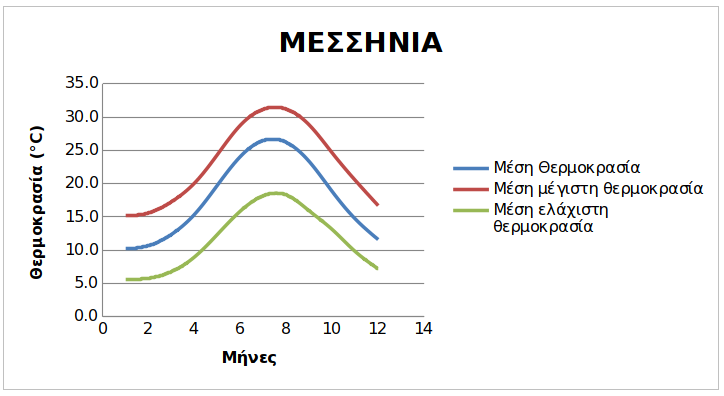
\includegraphics [scale = 0.80] {messinia4.png}
		\end{center}
	\end{figure}

	Αντίθετα η Αρκαδία έχει κλίμα ορεινό και το ετήσιο θερμομετρικό εύρος κυμαίνεται περίπου μεταξύ των $5 - 26^o C$. Ο χειμώνας στο νομό είναι ψυχρός, αρκετά ψυχρότερος από τη Μεσσηνία, ενώ το καλοκαίρι αρκετά δροσερό. Η ψυχρή περίοδος διαρκεί από το Οκτώβριο έως τον Απρίλιο και η θερμή από το Μάιο έως τον Σεπτέμβριο. Όσον αφορά την μέση μηνιαία θερμοκρασία κατά τη διάρκεια του έτους, η ελάχιστη παρουσιάζεται τους μήνες Δεκέμβριο και Ιανουάριο με περίπου $1^o C$ και η μέγιστη τους μήνες Ιούλιο και Αύγουστο με $30^o C$. 
	
	\begin{figure} [H]
		\begin{center}
			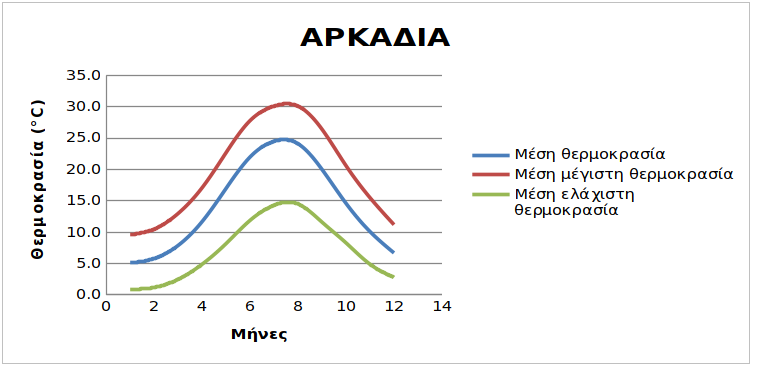
\includegraphics [scale = 0.80] {arkadia4.png}
		\end{center}
	\end{figure}

	\textbf{Βροχόπτωση}
	
	Όπως αναφέρθηκε ο νομός Μεσσηνίας έχει υγρό κλίμα με τις περισσότερες βροχοπτώσεις να εκδηλώνονται κατά τους χειμερινούς μήνες. Σύμφωνα με στοιχεία της ΕΜΥ το εύρος του ύψους βροχής του νομού κυμαίνεται περίπου μεταξύ $5-155 mm$. Τα μέγιστα ύψη εμφανίζονται μεταξύ Οκτωβρίου και Φεβρουαρίου ενώ τα ελάχιστα μεταξύ Μαρτίου και Σεπτεμβρίου. 
	
	\begin{figure} [H]
		\begin{center}
			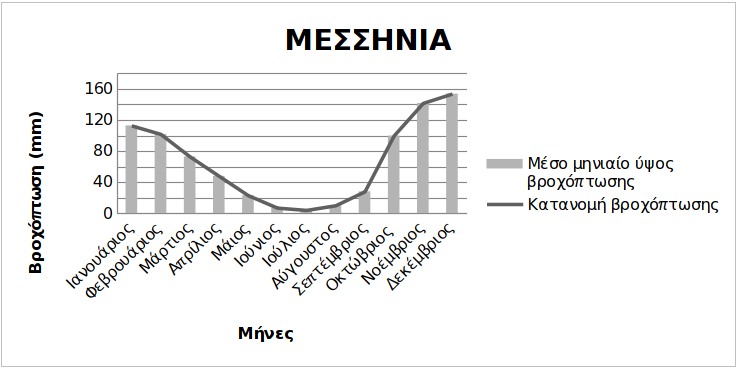
\includegraphics [scale = 0.80] {messinia5.png}
		\end{center}
	\end{figure}

	Αντίθετα η Αρκαδία που έχει ορεινό κλίμα έχει πιο έντονες βροχοπτώσεις κατά τη διάρκεια του έτους. Σύμφωνα με στοιχεία της ΕΜΥ το εύρος του ύψους βροχής του νομού κυμαίνεται περίπου μεταξύ $15-150 mm$. Τα μέγιστα ύψη εμφανίζονται μεταξύ Νοεμβρίου και Φεβρουαρίου ενώ τα ελάχιστα μεταξύ Μαρτίου και Οκτωβρίου. Συνολικά στην Αρκαδία εκδηλώνεται μέσο ετήσιο ύψος βροχόπτωσης περίπου $811 mm$.
	
	\begin{figure} [H]
		\begin{center}
			\includegraphics [scale = 0.80] {arkadia5.png}
		\end{center}
	\end{figure}

	\textbf{Σχετική υγρασία}
	
	Στο νομό Μεσσηνίας η μέση ετήσια σχετική υγρασία σχετική υγρασία φτάνει το 68\% με ξηρότερο μήνα τον Ιούλιο (58\%) και υγρότερους μήνες τον Νοέμβριο και τον Δεκέμβριο (75\%).
	
	\begin{figure} [H]
		\begin{center}
			\includegraphics [scale = 0.80] {messinia6.png}
		\end{center}
	\end{figure}

	Στο νομό Αρκαδίας η μέση ετήσια σχετική υγρασία σχετική υγρασία φτάνει το 63\% με ξηρότερο μήνα τον Ιούλιο (44\%) και υγρότερο τον Δεκέμβριο (78\%).
	
		\begin{figure} [H]
		\begin{center}
			\includegraphics [scale = 0.80] {arkadia6.png}
		\end{center}
	\end{figure}

	\textbf{Ένταση ανέμου}
	
	Η μέση μηνιαία ένταση του ανέμου στους δυο νομούς φαίνεται στα διαγράμματα που ακολουθούν.
	
	\begin{figure} [H]
		\begin{center}
			\includegraphics [scale = 0.80] {messinia7.png}
		\end{center}
	\end{figure}
	\begin{figure} [H]
		\begin{center}
			\includegraphics [scale = 0.80] {arkadia7.png}
		\end{center}
	\end{figure}

	\subsubsection{Ανθρωπογενές Περιβάλλον}
	
	\paragraph{Πληθυσμιακά στοιχεία}
	
	Σύμφωνα με την απογραφή της ΕΛΣΤΑΤ του 2011,ο μόνιμος πληθυσμός της Περιφέρειας Πελοποννήσου ανέρχεται σήμερα σε 577.903 άτομα με το 28\% στον Νομό Μεσσηνίας και το 15\% στο νομό Αρκαδίας.
	
	Η συγκέντρωση πληθυσμού στην Περιφέρεια έχει παραμείνει πρακτικά σταθερή την τελευταία δεκαετία (2001-2011), παρουσιάζοντας μία ελαφρά μείωση της τάξης του 3,0\%, ήτοι 0,3\% ετησίως.
	
	Αναλυτικά η ποσοστιαία μείωση του πληθυσμού στη δεκαετία 2001-2011, ήταν 4\% (ήτοι 0,4\% ετησίως) για το νομό Μεσσηνίας.
	
	Αναλυτικά, η κατανομή και εξέλιξη πληθυσμού ανά Δήμο και Δημοτική Ενότητα στη 2η υποενότητα παρουσιάζονται στον πίνακα που ακολουθεί:
	
	\begin{table}[H]
		\centering
		\begin{tabular}{|c|c|}
			\hline
			\textbf{ΠΕΡΙΦΕΡΕΙΑΚΗ ΕΝΟΤΗΤΑ} & \textbf{ΠΛΗΘΥΣΜΟΣ 2011} \\ \hline
			\textbf{Π.Ε ΑΡΚΑΔΙΑΣ} & \textbf{86685} \\ \hline
			Δ.ΓΟΡΤΥΝΙΑΣ & 10109 \\ \hline
			Δ.ΜΕΓΑΛΟΠΟΛΗΣ & 10687 \\ \hline
			\textbf{Π.Ε ΜΕΣΣΗΝΙΑΣ} & \textbf{159954} \\ \hline
			Δ.ΚΑΛΑΜΑΤΑΣ & 69849 \\ \hline
			Δ.ΜΕΣΣΗΝΗΣ & 23482 \\ \hline
			Δ.ΟΙΧΑΛΙΑΣ & 11228 \\ \hline
			Δ.ΠΥΛΟΥ-ΝΕΣΤΟΡΟΣ & 21077 \\ \hline
			Δ.ΤΡΙΦΥΛΙΑΣ & 27373 \\ \hline
			Δ.ΔΥΤΙΚΗΣ ΜΑΝΗΣ & 6945 \\ \hline
		\end{tabular}
		\caption{The caption}
		\label{The label}
	\end{table}
	
	\paragraph{Χρήσεις γης}
	
	\begin{figure} [H]
		\begin{center}
			\includegraphics [scale = 0.80] {xriseis3.png}
			\caption{Χρήσεις γης}
		\end{center}
	\end{figure}

	\paragraph{Πολιτιστική Κληρονομιά}
	
	\textbf{Περιοχές αρχαιολογικού και ιστορικού ενδιαφέροντος}
	
	Η Μεσσηνία και η Αρκαδία κατοικούνται εδώ και χιλιάδες χρόνια, με μία σπουδαία ιστορία να τις συνοδεύει. Μάρτυρες της ιστορίας τους, τα κλασσικά, βυζαντινά και νεότερα μνημεία που βρίσκονται στο έδαφός τους. Τα μνημεία και η πολιτιστική κληρονομιά της δεύτερης υποενότητας, σε συνδυασμό με το πανέμορφο φυσικό τοπίο που τα πλαισιώνει, δίνουν μία μαγική δύναμη στην περιοχή. Συγκεκριμένα τα μνημεία της δεύτερης υποενότητας είναι τα εξής:
	
	\begin{figure} [H]
		\begin{center}
			\includegraphics [scale = 0.80] {mnimia1.png}
			\caption{Αρχαιολογικοί χώροι Αρκαδίας}
		\end{center}
	\end{figure}

	\begin{figure} [H]
		\begin{center}
			\includegraphics [scale = 0.80] {mnimia2.png}
			\caption{Αρχαιολογικοί χώροι Μεσσηνίας}
		\end{center}
	\end{figure}

	\textbf{Παραδοσιακοί οικισμοί Νομού Μεσσηνίας}
	
	\begin{table}[H]
		\centering
		\begin{tabular}{|c|c|}
			\hline
			\textbf{1} & ΘΑΛΑΜΑΙ(ΚΟΥΤΗΦΑΡΙ) \\ \hline
			\textbf{2} & ΚΑΛΑΜΑΤΑ(ΤΜΗΜΑ ΤΗΣ ΠΟΛΗΣ) \\ \hline
			\textbf{3} & ΛΑΓΚΑΔΑ \\ \hline
			\textbf{4} & ΜΥΣΤΡΑΚΙΟΝ \\ \hline
			\textbf{5} & ΠΥΛΟΣ \\ \hline
		\end{tabular}
		\caption{Παραδοσιακοί οικισμοί Νομού Μεσσηνίας}
		\label{The label}
	\end{table}
	
	\subsection{3η Υποενότητα}
	
	\subsubsection{Φυσικό Περιβάλλον}
	
	\paragraph{Ανάγλυφο}
	
	\textbf{Γεωγραφία}
	
	Η Τρίτη υποενότητα αποτελείται αποκλειστικά από το νομό Λακωνίας. Ο νομός Λακωνίας βρίσκεται στο νοτιοανατολικό άκρο της Περιφέρειας Πελοποννήσου, έχει έκταση 3.636 τ.χλμ, 89.138 κατοίκους (\emph{Απογραφή 2011}) και έδρα τη Σπάρτη. Στα βόρεια συνορεύει με το νομό Αρκαδίας και στα δυτικά με το νομό Μεσσηνίας. Διαθέτει συνολικά πέντε δήμους, οι οποίοι είναι οι εξής:
	
	\begin{table}[H]
		\centering
		\begin{tabular}{|c|c|}
			\hline
			\textbf{Α/Α} & \textbf{Δήμος} \\ \hline
			1 & Ανατολικής Μάνης \\ \hline
			2 & Ελαφονήσου \\ \hline
			3 & Ευρώτα \\ \hline
			4 & Μονεμβασιάς \\ \hline
			5 & Σπάρτης \\ \hline
		\end{tabular}
		\caption{Δήμοι Νομού Λακωνίας}
		\label{The label}
	\end{table}
	
	Όπως φαίνεται στον γεωμορφολογικό χάρτη (βλ. σελίδα \pageref{peloponnese}) της Πελοποννήσου ο νομός έχει κατά βάση ορεινή έκταση με δυο βασικές οροσειρές στα σύνορα με την Αρκαδία και τη Μεσσηνία, τον Πάρνωνα και τον Ταΰγετο, αντίστοιχα. Ο Ταΰγετος (2406μ) και ο Πάρνωνας (1935μ) είναι οι δύο σημαντικότεροι ορεινοί όγκοι του νομού  με κατεύθυνση από τα βορειοδυτικά προς τα νοτιοανατολικά και καταλαμβάνουν σημαντικό μέρος της έκτασής του. Υπάρχει επίσης και το όρος Κρίθινο (773μ) στο Δήμο Μονεμβασιάς στο νοτιοανατολικό άκρο της Λακωνίας. Μοναδικός μεγάλος ποταμός είναι ο Ευρώτας που διασχίζει την κοιλάδα που ορίζουν ο Πάρνωνας και ο Ταΰγετος. Μικρότερα ποτάμια είναι ο Πλατύς ποταμός και ο Αρδέλης Ποταμός. Ο νομός διαθέτει έναν σημαντικό κάμπο, τον κάμπο του Ευρώτα, που ορίζεται από τον Πάρνωνα και τον Ταΰγετο στο κέντρο του νομού και εκτείνεται από Βορρά προς Νότο. 
	
	\textbf{Ακτογραφία}
	
	Ο νομός Λακωνίας, καθότι βρίσκεται στο νοτιοανατολικό άκρο της Πελοποννήσου, διαβρέχεται από θάλασσα στα νότια, στα ανατολικά και σε ένα πολύ μικρό κομμάτι στα δυτικά (βλ. σελίδα \pageref{peloponnese}). Συγκεκριμένα στα ανατολικά επικοινωνεί με το Μυρτώο Πέλαγος και στα νότια και νοτιοδυτικά με τη Μεσόγειο Θάλασσα. Η δυτική ακτογραμμή ξεκινά από τον Όρμο Λιμενίου στο Μεσσηνιακό κόλπο και συνεχίζοντας νότια συναντά τον Όρμο Δυρού, τον Όρμο Γερολιμένα και το Ακρωτήριο Ταίναρο, το οποίο αποτελεί και το σημείο έναρξης του Λακωνικού κόλπου. Από το σημείο αυτό ξεκινά η κίνηση προς το Βορρά με αρκετές ανωμαλίες και αφού σχηματιστεί ο Όρμος Σκουταρίου εμφανίζεται ο Όρμος Γυθείου. Από το σημείο αυτό η ακτογραμμή ξεκινά να κατευθύνεται προς τα ανατολικά χωρίς ιδιαίτερες μεταβολές και μετά τη διασταύρωσή της με τις εκβολές των ποταμών Πλατύ, Αρδέλη και το δέλτα του Ευρώτα αρχίζει την κίνηση προς το Νότο, όπου μετά τον Όρμο Ξυλί και τα ακρωτήρια Ξυλί και Αρχάγγελος καταλήγει στον Όρμο της Νεάπολης όπου βρίσκεται και η Νήσος Ελαφόνησος. Στη συνέχεια η ακτογραμμή φτάνει το νοτιότερο τμήμα του νομού, όπου βρίσκεται το ακρωτήριο Μαλέας, και ξεκινά να κατευθύνεται βόρεια κατά μήκος του κόλπου Επιδαύρου Λιμηράς και αφού συναντήσει τον Όρμο της Μονεμβασιάς καταλήγει στον Όρμο Κυπαρίσσου, μετά τον οποίο νότια του Όρμου Φωκιανού τερματίζεται. 
	
	\paragraph{Έδαφος-Γεωλογία-Υδάτινο Περιβάλλον}
	
	\textbf{Έδαφος}
	
	Σύμφωνα με την ταξινόμηση των εδαφών (βλ. σελίδα \pageref{edafi}), βάσει του συστήματος FAO (Χάρτης Εδαφών Ελλάδας – Εθνική Επιτροπή κατά της Ερημοποίησης – Γεωπονικό Πανεπιστήμιο Αθηνών – Συντάκτης Ν. Γιάσογλου – ( Παράρτημα IΙ ), τα εδάφη της τρίτης υποενότητας ταξινομούνται σε έξι κατηγορίες εδαφών, οι οποίες είναι:
	
	\begin{itemize}
		\item \emph{Βράχοι}(Rock Outcrops) (μαύρο χρώμα)
		\item \emph{\selectlanguage{english}Leptosols}\selectlanguage{english}(LP): \selectlanguage{greek}Εδάφη με μητρικό υλικό από ασβεστόλιθο και φλύσχη. Είναι λεπτόκοκκα εδάφη, αργιλώδη, καλής υδατοπερατότητας με ουδέτερο \selectlanguage{english}pH. \selectlanguage{greek}(γκρι χρώμα)
		\item \emph{\selectlanguage{english}Regosols}\selectlanguage{english}(RG): \selectlanguage{greek}Στρώμα χαλαρού υλικού, πάνω σε σκληρό υπόβαθρο. Είναι εδάφη μετρίως αργιλώδη, με μέτρια υδατοπερατότητα και με \selectlanguage{english}pH $>$ 7.\selectlanguage{greek}(κίτρινο χρώμα)
		\item \emph{\selectlanguage{english}Fluvisols}\selectlanguage{english}(FL): \selectlanguage{greek}Εδάφη αργιλώδη, με μέτρια έως μικρή υδατοπερατότητα και με \selectlanguage{english}pH $>$ 7.\selectlanguage{greek}(μπλε χρώμα)
		\item \emph{\selectlanguage{english}Cambisols}\selectlanguage{english}(CM): \selectlanguage{greek}Η σύσταση των εδαφών αυτών είναι αργιλλώδης και μετρίως αργιλλώδης, με μικρή υδατοπερατότητα και με ουδέτερο ή ελαφρώς όξινο \selectlanguage{english}pH. \selectlanguage{greek}(πορτοκαλί χρώμα)
	\end{itemize}

	Συμπερασματικά λοιπόν και σύμφωνα με τα παραπάνω στοιχεία το έδαφος της τρίτης υποενότητας  είναι αργιλώδες έως μετρίως αργιλώδες  με ουδέτερο προς αλκαλικό \eng pH.\gr Τα εδάφη της Λακωνίας είναι κατά κύριο λόγο υδατοπερατά κυρίως στο ανατολικό και κεντρικό τμήμα του νομού, ενώ στο νοτιοδυτικό τμήμα του νομού συναντάται βραχώδες έδαφος. 
	
	Η παραπάνω ανάλυση των εδαφών είναι από το βιβλίο Μαθήματα Εφαρμοσμένης Εδαφολογίας του Νικολάου Ιωάν Γιάσογλου (Αθήνα  Ιανουάριος 1995)
	
	Όπως φαίνεται στο χάρτη δυνητικού κινδύνου ερημοποίησης της Ελλάδας (βλ. σελίδα \pageref{erimopoiisi}) που συνετάχθη από την Εθνική Επιτροπή κατά της Ερημοποίησης το έδαφος της τρίτης υποενότητας κατατάσσεται ως μετρίου κινδύνου στο κεντρικό τμήμα του νομού Λακωνίας και υψηλού κινδύνου στα βόρεια, ανατολικά και νοτιοανατολικά, καθώς και στα δυτικά-νοτιοδυτικά.
	
	\textbf{Γεωλογία-Τεκτονική: Γεωτεκτονικές ζώνες Τρίτης Υποενότητας}
	
	Οι γεωτεκτονικές ζώνες που εμφανίζονται στην Τρίτη υποενότητα (βλ. σελίδα \pageref{geotektonikes}) είναι οι εξής:
	
	\begin{enumerate}
		\item \textbf{Ζώνη Ολωνού-Πίνδου} \\
		Κατέχει κεντρική θέση στον κορμό της Ελλάδας και ακολουθεί την κάμψη του ορογενετικού τόξου, ενώ τμήματα της απαντούν στην Κρήτη και τη Ρόδο. Συνίσταται από ασβεστόλιθους, δολομίτες, κερατόλιθους, ηφαιστειοϊζηματογενή πετρώματα, ραδιολαρίτες, αργίλους, ψαμμίτες και πηλίτες. Έχει επωθηθεί προς τα δυτικά πάνω στη ζώνη Γαβρόβου-Τριπόλεως και χαρακτηρίζεται από δομή λεπίων, με αποτέλεσμα συχνές επαναλήψεις των στρωμάτων. Πάνω στη ζώνη της Πίνδου βρίσκονται επωθημένες οι μεγαλύτερες οφιολιθικές μάζες του ελληνικού χώρου.
		\item \textbf{Ζώνη Γαβρόβου-Τριπόλεως} \\
		Η ζώνη Γαβρόβου - Τριπόλεως χαρακτηρίζεται από συνεχή ανθρακική ιζηματογένεση με κυρίαρχα πετρώματα τους ασβεστόλιθους και δολομίτες. Οι σχηματισμοί της ζώνης αυτής επικάθονται σε ένα υπόβαθρο αποτελούμενο από φυλλίτες, χαλαζιακούς φυλλίτες και μάρμαρα, γνωστό ως «φυλλιτική-χαλαζιτική» σειρά. Τα στρώματά της σχηματίζουν μεγάλα ανοικτά σύγκλινα και αντίκλινα και είναι επωθημένη δυτικά πάνω στην Ιόνιο ζώνη.
		\item \textbf{Ζώνη Παξών (ή Προαπούλια)} \\
		Είναι η  πιο εξωτερική γεωτεκτονική ζώνη της Ελλάδας, της οποίας εμφανίζεται  ένα μικρό τμήμα στα Ιόνια νησιά. Χαρακτηρίζεται από μια συνεχή νηριτική ιζηματογένεση και την απουσία φλύσχη.  Τα παλαιότερα πετρώματα είναι γύψοι και ακολουθούν δολομίτες, ασβεστόλιθοι, μαργαϊκοί ασβεστόλιθοι, μάργες και κερατόλιθοι. Θεωρείται ως αυτόχθονη ζώνη, το μεγαλύτερο τμήμα της οποίας είναι βυθισμένο στη θάλασσα, μεταξύ των ιόνιων νησιών και της Απουλίας (στην Νότιο Ιταλία).
	\end{enumerate}

	\textbf{Υδάτινο Περιβάλλον}
	
	Η τρίτη υποενότητα ανήκει εξ ολοκλήρου στο Υδατικό Διαμέρισμα Ανατολικής Πελοποννήσου που έχει έκταση 8007,42τ.χλμ (βλ. σελίδα \pageref{ydatika}). Ο υδροκρίτης του υδατικού διαμερίσματος ξεκινά από το όρος Δίδυμο συνεχίζει στο όρος Αραχναίο και αφού περάσει από τα όρη Ολίγυρτος Τραχύ, Λύρκειο και Αρτεμίσιο διακλαδώνεται στους υδροκρίτες των βουνών Ταΰγετος και Πάρνωνας. Σημαντικότερος ποταμός του νομού Λακωνίας είναι ο Ευρώτας που πηγάζει από το αρκαδικό οροπέδιο, νότια της Μαντινείας. Μετά από μία διαδρομή 82 χλμ., στην κοιλάδα που ορίζουν ο Πάρνωνας και ο Ταΰγετος, κατά μήκος της οποίας δέχεται τα νερά από αρκετούς παραποτάμους, εκβάλλει στο Λακωνικό Κόλπο. Μικρότερος ποταμός είναι ο Πλατύς ποταμός που πηγάζει από τον Ταΰγετο και αφού διασχίσει μέρος του δήμου Δυτικής Μάνης εκβάλλει στο Λακωνικό κόλπο νοτιοδυτικά του Μαυροβουνίου και ο Αρδέλης Ποταμός, που πηγάζει στα οροπέδια δυτικά της Σκάλας Λακωνίας και εκβάλλει στο Λακωνικό κόλπο στο ύψος της Σελινίτσας. Σημαντικότερη λίμνη του νομού είναι η λίμνη Στρογγύλη απέναντι από την Ελαφόνησο. Ως προς τα υπόγεια νερά (βλ. σελίδα \pageref{ypogeia}) ο νομός Λακωνίας έχει ορισμένες εκτάσεις με πλούσιο υπόγειο υδροφόρο ορίζοντα, οι οποίες καλύπτουν κατά βάση το κέντρο της Περιφερειακής Ενότητας.
	
	\paragraph{Σεισμική Επικινδυνότητα}
	
	Όπως φαίνεται και στον χάρτη σεισμικής επικινδυνότητας (βλ. σελίδα \pageref{seismiki}) η τρίτη υποενότητα δεν διατρέχει ιδιαίτερα σοβαρό κίνδυνο σε περίπτωση σεισμού. Συγκεκριμένα το δυτικό τμήμα του νομού Λακωνίας χαρακτηρίζεται  ως ζώνη μέτριου κινδύνου, ενώ το υπόλοιπο τμήμα του νομού ανήκει στη ζώνη χαμηλού κινδύνου. Ως προς τον κίνδυνο κατολίσθησης (βλ. σελίδα \pageref{katolisthiseis}) η τρίτη υποενότητα εντάσσεται εξ ολοκλήρου στη ζώνη μηδαμινής επικινδυνότητας.
	
	\paragraph{Οικότοποι-Χλωρίδα-Πανίδα}
	
	\textbf{Τύποι οικοσυστημάτων}
	
	Στο έδαφος του νομού Λακωνίας συνυπάρχουν διάφοροι τύποι οικοσυστημάτων. Σημαντικότερους από αυτούς είναι τα δάση, οι οικότοποι γλυκών υδάτων, οι βραχώδεις οικότοποι και τα σπήλαια καθώς και φυσικές και ημιφυσικές χλοώδεις διαπλάσεις και ρέοντα ύδατα.
	
	\textbf{Χλωρίδα-Πανίδα}
	
	Ο νομός Λακωνίας διαθέτει ποικιλία ειδών χλωρίδας και πανίδας, τα οποία μπορεί να διαφοροποιούνται από νομό σε νομό και κυρίως με τις εναλλαγές τύπου οικοσυστήματος από χερσαίο σε υδάτινο και από ηπειρωτικό σε παραλιακό.
	
	\textbf{Ευαίσθητες και Προστατευόμενες περιοχές}
	
	\begin{table}[H]
		\centering
		\begin{tabular}{|c|c|}
			\hline
			\multicolumn{2}{|c|}{\textbf{\eng NATURA 2000 \gr}} \\
			\textbf{ΚΩΔΙΚΟΣ} & \textbf{ΟΝΟΜΑ} \\ \hline
			\eng GR2540003 \gr & Εκβολές Ευρώτα \\ \hline
			\eng GR2540008 \gr & Νότια Μάνη \\ \hline
			\eng GR2540007 \gr & Όρη ανατολικής Λακωνίας \\ \hline
			\eng GR2540001 \gr & Όρη Γιδοβούνι, Χιονοβούνι, \\ & Γαϊδουροβούνι, Κοράκια, Καλογεροβούνι, \\ & Κουλοχέρα και περιοχή Μονεμβασιάς \\ \hline
			\eng GR2520006 \gr & Όρος Πάρνωνας (και περιοχή Μαλεβής) \\ \hline
			\eng GR2550006 \gr & Όρος Ταΰγετος \\ \hline
			\eng GR2550009 \gr & Όρος Ταΰγετος-Λαγκάδα Τρύπης \\ \hline
			\eng GR2540002 \gr & Περιοχή Νεάπολης και Νήσος Ελαφόνησος \\ \hline
			\eng GR2540006 \gr & Υγρότοποι εκβολών Ευρώτα \\ \hline
		\end{tabular}
		\caption{\eng NATURA 2000 \gr}
		\label{The label}
	\end{table}
	
	\begin{table}[H]
		\centering
		\begin{tabular}{|c|c|}
			\hline
			\multicolumn{2}{|c|}{\textbf{ΚΑΤΑΦΥΓΙΑ ΑΓΡΙΑΣ ΖΩΗΣ}} \\
			\textbf{ΚΩΔΙΚΟΣ} & \textbf{ΟΝΟΜΑ} \\ \hline
			Κ471 & Κάμπος Καρυών \\ \hline
			Κ474 & Σελλασίας-Βρεσθένων \\ \hline
			Κ475 & Κουφοβούνι-Τσικούλιο \\ \hline
			Κ510 & Αναδασώσεις \\ \hline
			Κ517 & Λουτσάκα-Χαμοσπηλιά-Πέρα Βρύση \\ \hline
			Κ497 & Κάστρο Γερακίου \\ \hline
			Κ778 & Γαϊδουροβούνι \\ \hline
			Κ776 & Ξυλί Ασωπού \\ \hline
			Κ775 & Κάτω Κορογόνα \\ \hline
			Κ524 & Πράταγος-Αετοφωλιά \\ \hline
			Κ777 & Βαβίλα-Κούνος Νεαπόλεως \\ \hline
			Κ924 & Πρασονήσι Κυθήρων \\ \hline
		\end{tabular}
		\caption{Καταφύγια Άγριας Ζωής}
		\label{The label}
	\end{table}
	
	\begin{table}[H]
		\centering
		\begin{tabular}{|c|c|}
			\hline
			\multicolumn{2}{|c|}{\textbf{ΤΟΠΙΑ ΙΔΙΑΙΤΕΡΟΥ ΦΥΣΙΚΟΥ ΚΑΛΟΥΣ}} \\
			\textbf{ΚΩΔΙΚΟΣ} & \textbf{ΟΝΟΜΑ} \\ \hline
			ΑΤ1011082 & Αρεόπολη \\ \hline
			ΑΤ1011076 & Βάθεια \\ \hline
			ΑΤ1010008 & Γύθειο \\ \hline
			ΑΤ1010011 & Κεντρικός Ταΰγετος \\ \hline
			ΑΤ1011077 & Κίττα \\ \hline
			ΑΤ1080121 & Λαγκάδα Ταϋγέτου \\ \hline
			ΑΤ1011068 & Μίνα Μάνης \\ \hline
			ΑΤ1010010 & Μονεμβασιά \\ \hline
			ΑΤ1080120 & Περιοχή Μυστρά-Παρορίου-Αγίου Ιωάννου \\ \hline
		\end{tabular}
		\caption{Τοπία Ιδιαίτερου Φυσικού Κάλλους}
		\label{The label}
	\end{table}
	
	\begin{table}[H]
		\centering
		\begin{tabular}{|c|c|}
			\hline
			\multicolumn{2}{|c|}{\textbf{ΒΙΟΤΟΠΟΙ \eng CORINE \gr}} \\
			\textbf{ΚΩΔΙΚΟΣ} & \textbf{ΟΝΟΜΑ} \\ \hline
			Α00010063 & Βουνά Μονεμβασιάς \\ \hline
			Α00010061 & Εκβολές Ευρώτα (Διβάρι και Λίμνη Αστερίου) \\ \hline
			Α00020021 & Ελαφόνησος Λακωνίας \\ \hline
			Α00030042 & Λίμνη Στρογγύλη (Βιγκλάφια) \\ \hline
			Α00010222 & Νότια Μάνη, Όρος Σαγγιάς και Ακρωτήριο Ταίναρο \\ \hline
			Α00010062 & Όρη Γιδοβούνι, Χιονοβούνι, Γαϊδουροβούνι, Κοράκια, Καλογεροβούνι, Κουλοχέρα \\ \hline
			Α00060092 & Όρος Πάρνωνας \\ \hline
			Α00060083 & Όρος Ταΰγετος \\ \hline
			Α00060082 & Χερσόνησος Μάνης \\ \hline
		\end{tabular}
		\caption{Βιότοποι \eng Corine \gr}
		\label{The label}
	\end{table}
	
	\paragraph{Κλιματολογικά και Μετεωρολογικά στοιχεία}
	
	\textbf{Κλίμα}
	
	Όπως φαίνεται και στον χάρτη, που απεικονίζει τις κλιματικές περιοχές της Ελλάδας, (βλ. σελίδα \pageref{klimatikes}) η τρίτη υποενότητα έχει κατά βάση υγρό μεσογειακό κλίμα με μέτριες βροχές, ήπιους χειμώνες και ξηρά καλοκαίρια με εξαίρεση το τμήμα της οροσειράς του Ταΰγετου που έχει ορεινό κλίμα με ψυχρούς χειμώνες, δροσερά καλοκαίρια και βροχές όλους τους μήνες του έτους. Συνεπώς η τρίτη υποενότητα ανήκει στην κλιματική ζώνη Α και σύμφωνα με την ενεργειακή ανάλυση των βαθμοημερών θέρμανσης (ΒΗΘ) (βλ. σελίδα \pageref{bathmoimeres}) χαρακτηρίζεται από 601-1100 ΒΗΘ.
	
	\textbf{Θερμοκρασια}
	
	Όπως αναφέρθηκε παραπάνω η Λακωνία έχει ήπιο εύκρατο κλίμα (εκτός φυσικά των ορεινών περιοχών που είναι πιο τραχύ), αφού σύμφωνα με στοιχεία της ΕΜΥ το ετήσιο θερμομετρικό εύρος κυμαίνεται περίπου μεταξύ των $11-24^o C$. Ο χειμώνας στο νομό είναι ήπιος, ενώ το καλοκαίρι εκτεταμένο και ξηρό. Η ψυχρή περίοδος διαρκεί από το Νοέμβριο έως τον Απρίλιο και η θερμή από το Μάιο έως τον Οκτώβριο. Όσον αφορά την μέση μηνιαία θερμοκρασία κατά τη διάρκεια του έτους, η ελάχιστη παρουσιάζεται τους μήνες Ιανουάριο και Φεβρουάριο με περίπου $4^o C$ και η μέγιστη τους μήνες Ιούλιο και Αύγουστο με $34^o C$. 
	
	\begin{figure} [H]
		\begin{center}
			\includegraphics [scale = 0.80] {sparth.png}
		\end{center}
	\end{figure}

	\textbf{Βροχόπτωση}
	
	\begin{figure} [H]
		\begin{center}
			\includegraphics [scale = 0.80] {sparti2.png}
		\end{center}
	\end{figure}
	
	Όπως αναφέρθηκε ο νομός Λακωνίας έχει υγρό κλίμα με τις περισσότερες βροχοπτώσεις να εκδηλώνονται κατά τους χειμερινούς μήνες. Σύμφωνα λοιπόν με τα στοιχεία της ΕΜΥ το εύρος του ύψους βροχής του νομού κυμαίνεται περίπου μεταξύ $5-150mm$. Τα μέγιστα ύψη εμφανίζονται μεταξύ Νοεμβρίου και Ιανουαρίου ενώ τα ελάχιστα μεταξύ Αυγούστου και Οκτωβρίου. 
	
	\textbf{Σχετική υγρασία}
	
	Στο νομό Λακωνίας η μέση ετήσια σχετική υγρασία σχετική υγρασία φτάνει το 60\% με ξηρότερο μήνα τον Ιούλιο (45,3\%) και υγρότερο μήνα τον Δεκέμβριο (72,8\%).
	
	\begin{figure} [H]
		\begin{center}
			\includegraphics [scale = 0.80] {sparti3.png}
		\end{center}
	\end{figure}

	\textbf{Ένταση ανέμου}
	
	Η μέση μηνιαία ένταση του ανέμου στο νομό φαίνεται στο διάγραμμα που ακολουθεί.
	
	\begin{figure} [H]
		\begin{center}
			\includegraphics [scale = 0.80] {sparti4.png}
		\end{center}
	\end{figure}

	\subsubsection{Ανθρωπογενές Περιβάλλον}
	
	\paragraph{Πληθυσμιακά στοιχεία}
	
	Σύμφωνα με την απογραφή της ΕΛΣΤΑΤ του 2011,ο μόνιμος πληθυσμός της Περιφέρειας Πελοποννήσου ανέρχεται σήμερα σε 577.903 άτομα με το 15\% στον Νομό Λακωνίας.
	
	Αναλυτικά, η κατανομή και εξέλιξη πληθυσμού ανά Δήμο και Δημοτική Ενότητα στη 2η υποενότητα παρουσιάζονται στον πίνακα που ακολουθεί:
	
	\begin{table}[H]
		\centering
		\begin{tabular}{|c|c|}
			\hline
			\textbf{ΠΕΡΙΦΕΡΕΙΑΚΗ ΕΝΟΤΗΤΑ} & \textbf{ΠΛΗΘΥΣΜΟΣ 2011} \\ \hline
			\textbf{ΛΑΚΩΝΙΑΣ} & \textbf{89138} \\ \hline
			Δ.ΑΝΑΤΟΛΙΚΗΣ ΜΑΝΗΣ & 13005 \\ \hline
			Δ.ΕΛΑΦΟΝΗΣΟΥ & 1041 \\ \hline
			Δ.ΕΥΡΩΤΑ & 17891 \\ \hline
			Δ.ΜΟΝΕΜΒΑΣΙΑΣ & 21942 \\ \hline
			Δ.ΣΠΑΡΤΗΣ & 35259 \\ \hline
		\end{tabular}
		\caption{Πληθυσμός Λακωνίας}
		\label{The label}
	\end{table}

	\paragraph{Χρήσεις γης}
	
	\begin{figure} [H]
		\begin{center}
			\includegraphics [scale = 0.80] {xriseis4.png}
			\caption{Χρήσεις Γης}
		\end{center}
	\end{figure}

	\paragraph{Πολιτιστική Κληρονομιά}
	
	\textbf{Περιοχές αρχαιολογικού και ιστορικού ενδιαφέροντος}
	
	Ο νομός Λακωνίας κατοικούνταν ήδη από την Εποχή του Χαλκού με αποτέλεσμα τη σημερινή εποχή  να είναι μια ζωντανή έκθεση μνημείων και ιστορικών χώρων. Πέρα από την πληθώρα εκκλησιών και ναών που σηματοδοτούν τη γέννησή τους στη βυζαντινή εποχή, στο έδαφος του νομού Λακωνίας υπάρχουν πάρα πολλά κτίσματα ιστορικού και αρχαιολογικού ενδιαφέροντος. Συγκεκριμένα τα μνημεία του νομού Λακωνίας είναι τα εξής:
	
	\begin{figure} [H]
		\begin{center}
			\includegraphics [scale = 0.80] {table1.png}
		\end{center}
	\end{figure}

	\textbf{Παραδοσιακοί οικισμοί}
	\begin{table}[H]
		\centering
		\begin{tabular}{|c|c|}
			\hline
			\textbf{Α/Α} & \textbf{Οικισμός} \\ \hline
			1 & ΑΓΙΟΣ ΙΩΑΝΝΗΣ ΖΑΡΑΚΑ \\ \hline
			2 & ΑΓΕΡΑΝΟΣ \\ \hline
			3 & ΑΓΙΟΣ ΑΘΑΝΑΣΙΟΣ \\ \hline
			4 & ΑΓΙΟΣ ΓΕΩΡΓΙΟΣ \\ \hline
			5 & ΑΛΙΚΑ \\ \hline
			6 & ΑΓΙΟΣ ΝΙΚΟΛΑΟΣ ΑΝ.ΜΑΝΗΣ \\ \hline
			7 & ΑΚΡΟΓΙΑΛΙΟΝ(ΠΙΟΝΤΕΣ,ΑΝΤΡΟΓΙΑΛΙ) \\ \hline
			8 & ΑΝΩ ΜΠΟΥΛΑΡΙΟΙ \\ \hline
			9 & ΑΝΩ ΓΑΡΔΕΝΙΤΣΑ \\ \hline
			10 & ΑΡΓΙΛΙΑ \\ \hline
			11 & ΑΡΕΟΠΟΛΙΣ \\ \hline
			12 & ΑΡΦΙΓΚΙΑ \\ \hline
			13 & ΑΡΙΑΝΑ ΖΑΡΑΚΑ \\ \hline
			14 & ΑΣΤΕΡΙΟΝ (ΤΑΣΟΛΑ) \\ \hline
			15 & ΑΧΙΛΛΕΙΟΝ \\ \hline
			16 & ΒΑΤΑ \\ \hline
			17 & ΒΑΘΕΙΑ \\ \hline
			18 & ΒΑΜΒΑΚΑ \\ \hline
			19 & ΒΑΧΟΣ \\ \hline
			20 & ΒΕΛΟΥΣΙ \\ \hline
		\end{tabular}
	\end{table}
	
	\begin{table}[H]
		\centering
		\begin{tabular}{|c|c|}
			\hline
			21 & ΓΕΡΜΑ \\ \hline
			22 & ΓΚΛΕΖΗ  (ΓΚΛΕΖΟΥ) \\ \hline
			23 & ΓΩΝΕΑ \\ \hline
			24 & ΔΙΜΑΡΙΣΤΙΚΑ \\ \hline
			25 & ΔΙΠΟΡΟΝ \\ \hline
			26 & ΔΡΟΣΟΠΗΓΗ \\ \hline
			27 & ΔΡΥ \\ \hline
			28 & ΔΡΥΑΛΟΣ ΟΙΤΥΛΟΥ \\ \hline
			29 & ΔΡΥΜΟΣ(ΔΡΥΑΛΙ) ΑΝ.ΜΑΝΗΣ \\ \hline
			30 & ΕΛΑΙΑ(ΕΛΙΑ) \\ \hline
			31 & ΕΞΩ ΝΥΜΦΙΟΝ \\ \hline
			32 & ΕΡΗΜΟΣ \\ \hline
			33 & ΙΕΡΑΚΑΣ ΖΑΚΑΡΑ \\ \hline
			34 & ΚΑΙΝΟΥΡΓΙΑ ΧΩΡΑ \\ \hline
			35 & ΚΑΛΟΝΙΟΙ \\ \hline
			36 & ΚΑΛΟΠΥΡΓΟΣ (ΑΝΩ ΔΡΥ) \\ \hline
			37 & ΚΑΛΟΣ \\ \hline
			38 & ΚΑΡΑΒΑΣ \\ \hline
			39 & ΚΑΡΕΑ (ΛΑΚΩΝΙΑΣ) \\ \hline
			40 & ΚΑΡΥΝΙΑ \\ \hline
			21 & ΓΕΡΜΑ \\ \hline
			22 & ΓΚΛΕΖΗ  (ΓΚΛΕΖΟΥ) \\ \hline
			23 & ΓΩΝΕΑ \\ \hline
			24 & ΔΙΜΑΡΙΣΤΙΚΑ \\ \hline
			25 & ΔΙΠΟΡΟΝ \\ \hline
			26 & ΔΡΟΣΟΠΗΓΗ \\ \hline
			27 & ΔΡΥ \\ \hline
			28 & ΔΡΥΑΛΟΣ ΟΙΤΥΛΟΥ \\ \hline
			29 & ΔΡΥΜΟΣ(ΔΡΥΑΛΙ) ΑΝ.ΜΑΝΗΣ \\ \hline
			30 & ΕΛΑΙΑ(ΕΛΙΑ) \\ \hline
			31 & ΕΞΩ ΝΥΜΦΙΟΝ \\ \hline
			32 & ΕΡΗΜΟΣ \\ \hline
			33 & ΙΕΡΑΚΑΣ ΖΑΚΑΡΑ \\ \hline
			34 & ΚΑΙΝΟΥΡΓΙΑ ΧΩΡΑ \\ \hline
			35 & ΚΑΛΟΝΙΟΙ \\ \hline
			36 & ΚΑΛΟΠΥΡΓΟΣ (ΑΝΩ ΔΡΥ) \\ \hline
			37 & ΚΑΛΟΣ \\ \hline
			38 & ΚΑΡΑΒΑΣ \\ \hline
			39 & ΚΑΡΕΑ (ΛΑΚΩΝΙΑΣ) \\ \hline
			40 & ΚΑΡΥΝΙΑ \\ \hline
		\end{tabular}
	\end{table}
	\begin{table}[H]
		\centering
		\begin{tabular}{|c|c|}
			\hline
			\textbf{41} & \textbf{ΚΑΡΥΟΥΠΟΛΙΣ} \\ \hline
			42 & ΚΑΥΚΙ \\ \hline
			43 & ΚΑΣΤΑΝΙΑ \\ \hline
			44 & Κ.ΓΑΡΔΕΝΙΤΣΑ \\ \hline
			45 & ΚΑΤΩ ΚΑΡΕΑ \\ \hline
			46 & ΚΑΤΩ ΜΠΟΥΛΑΡΙΟΙ \\ \hline
			47 & ΚΑΦΙΟΝΑ \\ \hline
			48 & ΚΕΛΕΦΑ \\ \hline
			49 & ΚΕΡΙΑ \\ \hline
			50 & ΚΕΧΡΙΑΝΙΚΑ \\ \hline
			51 & ΚΗΠΟΥΛΑ \\ \hline
			52 & ΚΙΤΤΑ \\ \hline
			53 & ΚΟΡΑΚΙΑΤΙΚΑ (ΚΟΡΑΚΙΑΝΙΚΑ) \\ \hline
			54 & ΚΟΡΟΓΟΝΙΑΝΙΚΑ \\ \hline
			55 & ΚΟΤΡΑΦΙΟΝ \\ \hline
			56 & ΚΟΥΛΟΥΜΙΟΝ \\ \hline
			57 & ΚΟΥΝΟΣ \\ \hline
			58 & ΚΟΥΤΡΕΛΑ \\ \hline
			59 & ΚΡΥΟΝΕΡΙΟΝ(ΛΑΚΩΝΙΑΣ) \\ \hline
			60 & ΚΥΠΑΡΙΣΣΙ ΖΑΡΑΚΑ \\ \hline
			61 & ΚΥΠΑΡΙΣΣΟΣ ΟΙΤΥΛΟΥ \\ \hline
			62 & ΛΑΓΙΑ \\ \hline
			63 & ΛΑΚΚΟΣ \\ \hline
			64 & ΛΑΜΠΟΚΑΜΠΟΣ ΖΑΡΑΚΑ \\ \hline
			65 & ΛΙΜΑΝΙ ΙΕΡΑΚΑ ΖΑΡΑΚΑ \\ \hline
			66 & ΛΟΓΓΑΡΙ ΖΑΡΑΚΑ \\ \hline
			67 & ΛΕΟΝΤΑΚΗΣ \\ \hline
			68 & ΛΙΜΕΝΙΟΝ \\ \hline
			69 & ΛΟΥΚΑΔΙΚΑ \\ \hline
			70 & ΜΑΛΛΙΑΡΗ ΣΥΚΙΑ \\ \hline
			71 & ΜΑΡΑΘΟΣ \\ \hline
			72 & ΜΕΖΑΠΟΣ \\ \hline
			73 & ΜΕΣΑ ΧΩΡΑ(ΜΕΣΑ ΝΥΦΗ) \\ \hline
			74 & ΜΙΝΑ \\ \hline
			75 & ΜΟΝΕΜΒΑΣΙΑ \\ \hline
			76 & ΜΟΥΝΤΑΝΙΣΤΙΚΑ \\ \hline
			77 & ΜΠΡΙΚΙΟΝ(ΒΡΙΚΙ) \\ \hline
			78 & ΝΙΚΑΝΔΡΕΙΟΝ \\ \hline
			79 & ΝΟΜΙΑ \\ \hline
			80 & ΟΙΤΥΛΟΝ \\ \hline
		\end{tabular}
	\end{table}

	\begin{table}[H]
		\centering
		\begin{tabular}{|c|c|}
			\hline
			81 & ΟΛΥΜΠΙΑΙ \\ \hline
			82 & ΟΜΑΛΑΙ \\ \hline
			83 & ΟΧΙΑ \\ \hline
			84 & ΠΑΓΚΙΑ \\ \hline
			85 & ΠΑΛΑΙΟΧΩΡΑ \\ \hline
			86 & ΠΑΛΙΡΟΣ \\ \hline
			87 & ΠΑΡΑΛΙΑ ΚΥΠΑΡΙΣΣΙΟΥ ΖΑΡΑΚΑ \\ \hline
			88 & ΠΑΧΙΑΝΙΚΑ \\ \hline
			89 & ΠΟΛΕΜΙΤΑΣ (ΠΟΛΕΜΙΤΑ) \\ \hline
			90 & ΠΟΛΥΧΡΑΒΟΣ \\ \hline
			91 & ΠΥΡΓΟΣ ΔΥΡΟΥ \\ \hline
			92 & ΠΥΡΡΙΧΟΣ \\ \hline
			93 & ΠΙΣΤΑΜΑΤΑ ΖΑΡΑΚΑ \\ \hline
			94 & ΡΕΙΧΙΑ ΖΑΡΑΚΑ \\ \hline
			95 & ΡΙΓΑΝΟΧΩΡΑ \\ \hline
			96 & ΣΚΑΛΤΣΟΤΙΑΝΙΚΑ \\ \hline
			97 & ΣΠΙΡΑ \\ \hline
			98 & ΣΤΑΥΡΙΟΝ \\ \hline
			99 & ΣΩΤΗΡΑΣ(ΚΟΥΣΚΟΥΝΙ) \\ \hline
			100 & ΤΣΙΚΚΑΛΙΑ \\ \hline
			101 & ΤΣΟΠΑΚΑΣ \\ \hline
			102 & ΤΡΙΑΝΤΑΦΥΛΛΙΑ \\ \hline
			103 & ΦΛΟΜΟΧΩΡΙΟΝ \\ \hline
			104 & ΦΡΑΓΚΟΥΛΙΑΣ \\ \hline
			105 & ΧΑΡΙΑ \\ \hline
			106 & ΧΑΡΟΥΔΑ \\ \hline
		\end{tabular}
		\caption{Παραδοσιακοί Οικισμοί Λακωνίας}
		\label{The label}
	\end{table}
	
	\subsection{Υφιστάμενη κατάσταση ρύπανσης}
	
	\subsubsection{Ατμοσφαιρικό-Ακουστικό περιβάλλον}
	
	Βασικοί ρύποι εκπέμπονται στην ατμόσφαιρα της Περιφέρειας Πελοποννήσου και ειδικότερα σε Μεγαλόπολη και Κόρινθο εξαιτίας της βιομηχανικής δραστηριότητας των  περιοχών καθώς και της αστικής ρύπανσης (κυκλοφορία οχημάτων και θέρμανση).Οι σημαντικότεροι εξ αυτών είναι: 
	
	\begin{itemize}
		\item Μονοξείδια του άνθρακα \eng (CO),\gr υδρογονάνθρακες \eng (HxCy)\gr και πτητικές οργανικές ενώσεις \eng (VOCs)\gr λόγω ατελούς καύσης των αγροτικών μηχανημάτων
		\item Διοξείδιο του θείου \eng(SO2)\gr, από πετρέλαιο και άλλα καύσιμα
		\item Σωματίδια και σκόνες προερχόμενα από το έδαφος
	\end{itemize}

	Ακολουθεί πίνακας στον οποίο απεικονίζεται η εκτίμηση εκπομπής των αερίων θερμοκηπίου ανά νομό της Περιφέρειας Πελοποννήσου. Ο πιο ρυπογόνος τομέας αυτός της ενέργειας.
	
	\begin{figure} [H]
		\begin{center}
			\includegraphics [scale = 0.60] {table2.png}
			\caption{Εκτίμηση εκπομπής των αερίων θερμοκηπίου ανά νομό της Περιφέρειας Πελοποννήσου}
		\end{center}
	\end{figure}

	\subsubsection{Υδατικοί πόροι}
	
	Ζήτηση νερού: \\
	Οι συνολικές ανάγκες σε νερό για όλες τις χρήσεις των ανθρώπινων δραστηριοτήτων υποδηλώνουν μεγάλη ζήτηση , πιο συγκεκριμένα :
	
	\begin{itemize}
		\item Υδατικό Διαμέρισμά Δυτικής Πελοποννήσου :: ΛΑΠ του Αλφειού 156 εκ.$m^3$ ανά έτος και στη ΛΑΠ Πάμισου– Νέδοντος –Νέδα 132,5 εκ.μ3 ανά έτος.
		\item Υδατικό Διαμέρισμά Ανατολικής Πελοποννήσου:ΛΑΠ ρεμάτων Οροπεδίου Τρίπολη 26εκ. $m^3$ ανά έτος και ΛΑΠ Ρεμάτων Αργολικού Κόλπου 284εκ. $m^3$ ανά έτος
 		\item Υδατικό Διαμέρισμά Βόρειας Πελοποννήσου: ΛΑΠ του Πηνειού - Πείρου - Βέργα 340εκ. $m^3$ ανά έτος και  Λεκάνη Απορροής Ρεμάτων Παραλίας Βορείου Πελοποννήσου 224,5εκ. $m^3$ ανά έτος.
	\end{itemize}
	
	Ποιότητα Επιφανειακών και Υπόγειων Υδάτων: \\
	Τόσο στο Υδατικό Διαμέρισμά Δυτικής Πελοποννήσου όσο και στο Υδατικό Διαμέρισμά Βόρειας Πελοποννήσου τα υδατικά συστήματα (ποτάμια, λίμνες,παράκτια) βρίσκονται στο σύνολο σε καλή κατάσταση ενώ υπάρχει ένα μεγάλο ποσοστό των οποίων η κατάσταση είναι μέτρια/κακή έως και άγνωστη.
	
	\subsubsection{Πιέσεις στο έδαφος}
	
	Οι σημαντικότερες πηγές ρύπανσης του εδάφους είναι τα αστικά λύματα , τα βιομηχανικά απόβλητα ,η απόθεση ΑΣΑ και τα γεωργικά απόβλητα. Ακολουθούν τα σημεία τα οποία εξακριβωμένα έχουν δεχτεί επιβάρυνση μέσω μετρήσεων και εργαστηριακών δοκιμών.
	
	\underline{Εγκαταστάσεις ΔΕΗ , Μεγαλόπολη}
	
	Στη Μεγαλόπολη βρίσκονταιοι εγκαταστάσεις της ΔΕΗ ΑΕ, οι οποίες περιλαμβάνουν τέσσερις Ατμοηλεκτρικούς Σταθμούς(ΑΗΣ)  ηλεκτροπαραγωγής και λιγνιτωρυχεία για την τροφοδοσία των σταθμών με καύσιμη ύλη. Οι δύο εκ των ΑΗΣ είναι ισχύος
	$125MW$, ο τρίτος $300MW$, και ο τέταρτος και πιο πρόσφατος ισχύος $300MW$. Κατά τη σταδιακή εξάντληση των αποθεμάτων λιγνίτη ανά περιοχές, άρχισε να γίνεται χρήση των εξαντλημένων ορυχείων για απόθεση παραπροϊόντων της εξόρυξης και υπολειμμάτων καύσης.
	
	\underline{Χώρος ανεξέλεγκτης διάθεσης απορριμμάτων (ΧΑΔΑ)}
	
	Η πρακτική αυτή εφαρμόζεται χρόνια στην Περιφέρεια και οι χώροι που χρησιμοποιούνται εντοπίζονται μέσα σε ρέματα ή πάνω από υδροφόρους ορίζοντες που τροφοδοτούν με πόσιμο νερό τις πόλεις .Έτσι έχει δημιουργήσει σε πολλές περιοχές σημαντικά προβλήματα ρύπανσης και κινδύνους για την υγεία των πολιτών. Παράλληλα οι Χώροι Ανεξέλεγκτης Διάθεσης Απορριμμάτων  (ΧΑΔΑ) συμβάλλουν στη δημιουργία εστιών πυρκαγιών. 
	
	Αναλυτικά οι Χώροι Ανεξέλεγκτης Διάθεσης Απορριμμάτων(ΧΑΔΑ) της περιφέρειας παρουσιάζονται σε επόμενο κεφάλαιο.
	
	\underline{Βιομηχανικές ζώνες}
	
	Ο Νομός Αρκαδίας και ο Νομός Κορινθίας αντιμετωπίζουν φαινόμενα ρύπανσης λόγω βιομηχανικών δραστηριοτήτων (ορυχεία , ηλεκτροπαραγωγή ΔΕΗ).
	
	\subsubsection{Πιέσεις στις ευαίσθητες και προστατευόμενες περιοχές}
	
	Η υπό εξέταση περιφέρεια παρουσιάζει μεγάλη ποικιλία φυσικών σχηματισμών οι κυριότερες κατηγορίες των οποίων είναι οι υγρότοποι και οι ορεινοί σχηματισμοί. Η υπερβολική χρήση νερού (απο γεωργικές καλλιέργειες κα) ασκεί πιέσεις στους υγρότοπους οι οποίες θέτουν σε κίνδυνο τα είδη της πανίδας και συγκεκριμένα αυτά που ζουν μέσα στους υγρότοπους. Ακόμα, η βόσκηση ,το κυνήγι, η παράνομη ξύλευση και ο τουρισμός ασκούν πιέσεις στους ορεινούς σχηματισμούς.Επιπρόσθετα τα μεγάλα οδικά έργα,όπως ο αυτοκινητόδρομος Τρίπολη – Καλαμάτα προκαλεί κινδύνους για την καταστροφή των βιοτόπων . Τέλος,επηρεάζεται η ποιότητα ζωής των κατοίκων των περιοχών της περιφέρειας. Η ζημιά στο τοπίο της περιοχής ,  η καταστροφή της φυσικής κάλυψης από πυρκαγιές που μπορούν να προκαλέσουν  πλημμύρες είναι μερικές σημαντικές καταστροφές. Αυτές έχουν ανυπολόγιστες συνέπειες για την τοπική οικονομία, την πρωτογενή παραγωγή (γεωργία, κτηνοτροφία), καθώς και τον τουρισμό.
	
	\section{Κατηγοριοποίηση Στερεών Αποβλήτων}
	
	\subsection{Τύποι Αποβλήτων}
	
	Σύμφωνα με τον ΠΕΣΔΑ 2010 τα απόβλητα χωρίζονται σε τέσσερις βασικές κατηγορίες: τα αστικού τύπου απόβλητα, τα βιομηχανικά απόβλητα, τα απόβλητα εκσκαφών κατασκευών και κατεδαφίσεων, καθώς και τα γεωκτηνοτροφικά απόβλητα.
	
	Στα \emph{απόβλητα αστικού τύπου} ταξινομούνται τα οικιακά απόβλητα, καθώς και αυτά που έχουν συναφή σύσταση, τα απόβλητα ηλεκτρικού και ηλεκτρονικού εξοπλισμού οικιακής προέλευσης, απόβλητα φορητών ηλεκτρικών στηλών και συσσωρευτών, οι μικρές ποσότητες επικίνδυνων αποβλήτων στα αστικά και τέλος οι ιλύες αστικού τύπου.
	
	Στα \emph{βιομηχανικά απόβλητα} κατατάσσονται τα απλά βιομηχανικά απόβλητα, τα απόβλητα εγκαταστάσεων κοινής ωφέλειας, τα απόβλητα λιπαντικά έλαια, τα απόβλητα συσσωρευτών οχημάτων και βιομηχανίας, τα οχήματα τέλους κύκλου ζωής, τα μεταχειρισμένα ελαστικά οχημάτων, τα απόβλητα ηλεκτρικού και ηλεκτρονικού εξοπλισμού βιομηχανικής προέλευσης, τα απόβλητα υγειονομικών μονάδων, τα ζωικά απόβλητα και τα απόβλητα που περιέχουν υδράργυρο.
	
	\subsection{Απόβλητα αστικού τύπου}
	
	\subsubsection{Οικιακά απόβλητα}
	
	Η σύσταση των οικιακών αποβλήτων δίνεται από το ΕΔΣΑ (διάγραμμα στόχων για το 2020):
	
	\begin{table}[H]
		\centering
		\begin{tabular}{|c||c|}
			\hline
			\textbf{ΥΛΙΚΟ} & \textbf{ΠΟΣΟΣΤΟ} \\ \hline
			Ζυμώσιμα & 44,3\% \\ \hline
			Χαρτί & 22,2\% \\ \hline
			Πλαστικό & 13,9\% \\ \hline
			Μέταλλο & 3,9\% \\ \hline
			Γυαλί & 4,3\% \\ \hline
			Ξύλο & 4,6\% \\ \hline
			Λοιπά & 6,8\% \\ \hline
		\end{tabular}
		\caption{Σύσταση Οικιακών Αποβλήτων}
		\label{The label}
	\end{table}
	
	Προκειμένου να καθοριστεί το φορτίο σχεδιασμού για τα έργα διαχείρισης αποβλήτων θα πρέπει πρώτα να ληφθούν υπόψη τα πληθυσμιακά δεδομένα. Αποφασίστηκε να γίνει χρήση της πρόβλεψης της \eng EUROSTAT \gr για τον εξυπηρετούμενο πληθυσμό του 2025, η οποία συνυπολογίζει τη μείωση του μόνιμου πληθυσμού από το 2011, οπότε και έγινε η τελευταία απογραφή της ΕΛΣΤΑΤ, καθώς και το τουριστικό φορτίο σε ένα βάθος χρόνου σχεδόν δεκαετίας. Τελικά ο πληθυσμός της Πελοποννήσου το έτος 2025 θεωρείται 560.479 κάτοικοι. Αναλυτικά:
	
	\begin{figure} [H]
		\begin{center}
			\includegraphics [scale = 0.35] {table3.png}
			\caption{Πληθυσμιακά Δεδομένα}
		\end{center}
	\end{figure}

	Στη συνέχεια πραγματοποιείται υπολογισμός της παραγόμενης ποσότητας ΑΣΑ με βάση τα Τοπικά Σχέδια Διαχείρισης σε έτος βάσης το 2014 και με ταυτόχρονη εκτίμηση της εξέλιξης της παραγωγής μέχρι το 2025 με βασική παράμετρο την εξέλιξη του ΑΕΠ καταλήγουμε σε φορτίο 277.596 τόνους για το έτος 2025 και συνεπώς φορτίο σχεδιασμού \emph{495,28 κιλά/κάτοικο/έτος}. Αναλυτικά:
	
	\begin{figure} [H]
		\begin{center}
			\includegraphics [scale = 0.45] {table4.png}
		\end{center}
	\end{figure}

	\underline{Φορτίο σχεδιασμού ανά διαχειριστική ενότητα}
	
	\begin{figure} [H]
		\begin{center}
			\includegraphics [scale = 0.45] {table5.png}
		\end{center}
	\end{figure}

	\subsubsection{Απόβλητα ηλεκτρικού και ηλεκτρονικού εξοπλισμού οικιακής προέλευσης}
	
	Ως ηλεκτρικός και ηλεκτρονικός εξοπλισμός οικιακής προέλευσης ορίζεται κατά το Άρθρο 3 της Οδηγίας 2012/19/ΕΕ ως ο εξοπλισμός, η ορθή λειτουργία του οποίου εξαρτάται από ηλεκτρικά ρεύματα ή ηλεκτρομαγνητικά πεδία και ο εξοπλισμός για την παραγωγή, τη μεταφορά και τη μέτρηση των ρευμάτων και πεδίων αυτών, ο οποίος έχει σχεδιασθεί για να λειτουργεί υπό ονομαστική τάση έως $1000V$ εναλλασσόμενου ρεύματος ή $1500V$ συνεχούς ρεύματος συμπεριλαμβανομένων όλων των κατασκευαστικών στοιχείων, των συναρμολογημένων μερών και των αναλωσίμων, που συνιστούν τμήμα του προϊόντος κατά το χρόνο απόρριψής του. \\
	Σύμφωνα με τον ΠΕΣΔΑ 2010:
	
	\begin{figure} [H]
		\begin{center}
			\includegraphics [scale = 0.45] {table6.png}
		\end{center}
	\end{figure}

	Τα απόβλητα ηλεκτρικού και ηλεκτρονικού εξοπλισμού οικιακής προέλευσης συλλέγονται και ανακυκλώνονται από διάφορες εταιρείες συλλογής και ανακύκλωσης συσκευών.
	
	\subsubsection{Απόβλητα φορητών ηλεκτρικών στηλών  και συσσωρευτών}
	
	Τα απόβλητα φορητών ηλεκτρικών στηλών και συσσωρευτών ρυθμίζεται από την ΚΥΑ 41624/2057/Ε103/2010 «Μέτρα, όροι και πρόγραμμα για την εναλλακτική διαχείριση των μεταχειρισμένων ηλεκτρικών στηλών και συσσωρευτών».
	
	\begin{figure} [H]
		\begin{center}
			\includegraphics [scale = 0.45] {table7.png}
		\end{center}
	\end{figure}

	Τα απόβλητα φορητών ηλεκτρικών στηλών και συσσωρευτών συλλέγονται και ανακυκλώνονται από τη ΣΕΑ ΑΦΗΣ ΑΕ που είναι ο εγκεκριμένος φορέας από το ΥΠΕΚΑ.
	
	\subsubsection{Μικρές ποσότητες επικίνδυνων αποβλήτων}
	
	Στην κατηγορία αυτή ανήκουν κυρίως χημικές ουσίες ή προϊόντα οικιακής χρήσης που περιέχουν τις ουσίες: αρσενικό, μόλυβδος, χρώμιο, κάδμιο, χαλκός, νικέλιο, υδράργυρος, ψευδάργυρος, βενζόλιο, κυανιούχο νάτριο, πολυχλώριωμένα διφαινύλια/τριφαινύλια, τετραχλωροαιθυλένιο, τριχλωροαιθυνλένιο και τετραχλωρομεθάνιο.
	
	\begin{figure} [H]
		\begin{center}
			\includegraphics [scale = 0.45] {table8.png}
		\end{center}
	\end{figure}

	\subsubsection{Ιλύες αστικού τύπου}
	
	Στην ενότητα αυτή ανήκουν οι ιλύες που προέρχονται από τις εγκαταστάσεις επεξεργασίας αστικών λυμάτων. 
	
	Η εκτιμώμενη παραγωγή ιλύος από ΕΕΛ ανά περιφερειακή ενότητα είναι: 
	\begin{itemize}
		\item ΠΕ Κορινθίας: 1916 τόνοι/έτος
		\item ΠΕ Αργολίδας: 2292 τόνοι/έτος
		\item ΠΕ Αρκαδίας: 551 τόνοι/έτος
		\item ΠΕ Μεσσηνίας: 1523 τόνοι/έτος
		\item ΠΕ Λακωνίας: 298 τόνοι/έτος
		\item Περιφέρεια Πελοποννήσου: 6580 τόνοι/έτος
	\end{itemize}
	
	Η εκτιμώμενη παραγωγή ξηράς ιλύος από δημοτικές εγκαταστάσεις είναι:
	
	\begin{itemize}
		\item ΠΕ Κορινθίας: 1797 τόνοι/έτος
		\item ΠΕ Αργολίδας: 1202 τόνοι/έτος
		\item ΠΕ Αρκαδίας: 1074 τόνοι/έτος
		\item ΠΕ Μεσσηνίας: 1981 τόνοι/έτος
		\item ΠΕ Λακωνίας: 1104 τόνοι/έτος
		\item Περιφέρεια Πελοποννήσου: 7157 τόνοι/έτος
	\end{itemize}
	Η εκτιμώμενη παραγωγή ξηράς ιλύος από τουριστικές εγκαταστάσεις είναι:
	\begin{itemize}
		\item ΠΕ Κορινθίας: 28 τόνοι/έτος
		\item ΠΕ Αργολίδας: 35 τόνοι/έτος
		\item ΠΕ Αρκαδίας: 5 τόνοι/έτος
		\item ΠΕ Μεσσηνίας: 29 τόνοι/έτος
		\item ΠΕ Λακωνίας: 13 τόνοι/έτος
		\item Περιφέρεια Πελοποννήσου: 110 τόνοι/έτος
	\end{itemize}

	\subsection{Βιομηχανικά απόβλητα}
	
	Στην περίπτωση των βιομηχανικών αποβλήτων βασική ευθύνη για την ορθή διαχείριση (εντός της εγκατάστασης) έχει ο παραγωγός του αποβλήτου. Σύμφωνα με το νόμο είναι υποχρεωμένος να διαχειριστεί τα παραγόμενα απόβλητα με σύννομο τρόπο και φέρει ευθύνη για τυχόν παρεκκλίσεις.
	
	\subsection{Απόβλητα εκσκαφών κατασκευών και κατεδαφίσεων}
	
	Στην κατηγορία αυτή ανήκουν υλικά εκσκαφών, κατασκευών, οδοποιίας και κατεδαφίσεων. Σύμφωνα με τον ΠΕΣΔΑ 2010 η μελλοντική εκτιμώμενη παραγωγή για το έτος 2020 φαίνεται στον παρακάτω πίνακα.
	
	\begin{figure} [H]
		\begin{center}
			\includegraphics [scale = 0.45] {table9.png}
		\end{center}
	\end{figure}

	Τα απόβλητα εκσκαφών, κατασκευών και κατεδαφίσεων συλλέγονται και επαναχρησιμοποιούνται από το ΣΣΕΔ Απόβλητα Εκσκαφών, Κατασκευών και Κατεδαφίσεων με διακριτικό τίτλο ΑΑΝΕΛ που είναι ο εγκεκριμένος φορέας από τον Ε.Ο.ΑΝ.
	
	\subsection{Γεωκτηνοτροφικά απόβλητα}
	
	Τα απόβλητα αυτά προέρχονται προφανώς από τις γεωργικές και κτηνοτροφικές δραστηριότητες.
	
	\begin{figure} [H]
		\begin{center}
			\includegraphics [scale = 0.50] {table10.png}
		\end{center}
	\end{figure}

	\section{Μηδενική Λύση}
	
	Ως πρώτο εναλλακτικό σενάριο προτείνεται η περίπτωση της «Μηδενικής Λύσης» (zero solution), σύμφωνα με την οποία διατηρείται η υφιστάμενη κατάσταση ως προς την μέχρι τώρα διαχείριση των αστικών απορριμμάτων, χωρίς την ύπαρξη καμίας κατασκευαστικής παρέμβασης. Αναφέρεται, δηλαδή, στην εκμετάλλευση των ήδη υπάρχουσων εγκαταστάσεων για την κατάληξη των απορριμμάτων της Περιφέρειας Πελοποννήσου. Οι εγκαταστάσεις που καταγράφονται αυτή την στιγμή στην Περιφέρεια είναι:
	
	\begin{itemize}
		\item Χώροι Ανεξέλεγκτης Διάθεσης Απορριμμάτων (Χ.Α.Δ.Α.)
		\item Χώροι Υγειονομικής Ταφής Απορριμμάτων (Χ.Υ.Τ.Α.)
		\item Μονάδες Κεντρικής Διαλογής Ανακυκλώσιμων Υλικών (Κ.Δ.Α.Υ.)
		\item Εργοστάσια Μηχανικης Ανακύκλωσης Κομποστοποίησης (Ε.Μ.Α.Κ.)
		\item Δεματοποιητές Σύμμεικτων Απορριμμάτων
	\end{itemize}

	\subsection{Χώροι Ανεξέλεγκτης Διάθεσης Απορριμμάτων (Χ.Α.Δ.Α.)}
	
	Ο όρος Χ.Α.Δ.Α. που είναι ευρέως γνωστός και ως «χωματερή», αναφέρεται σε χώρους όπου πραγματοποιείται ανεξέλεγκτη απόθεση σύμμεικτων απορριμμάτων, χώρίς προδιαγραφές, προκαλλώντας τη δημιουργία τρομερών εστιών μόλυνσης και υποβαθμίζοντας το φυσικό περιβάλλον της ευρύτερης περιοχής. Σύμφωνα με το ευρωπαικό και εθνικό μας δίκαιο, έχει απαγορευτεί επισήμως η ύπαρξη και χρήση τέτοιων χώρων για την κατάλληξη των αστικών απορριμμάτων. Η μέχρι στιγμής μη συμμόρφωσή μας έχει οδηγήσει στην επιβολή προστίμων που αφορούν σε μερικά δεκάδες εκατομμύρια ευρώ ετησίως, και η αποπληρωμή των οποίων επιμερίζεται τόσο στην Περιφέρεια (60\%), όσο και στους δήμους της (40\%). Όσον αφορά την Περιφέρεια Πελοποννήσου, παρά τη διαρκή μείωση του αριθμού των χωματερών της (που έχουν παύσει να λειτουργούν κι έχουν αποκατασταθεί), εξακολουθούν κάποιοι να υφίστανται. Οι υφιστάμενοι Χ.Α.Δ.Α. της ευρύτερης περιοχής της Περιφέρειας, σύμφωνα με την τελευταία λίστα που δόθηκε από τη Γενική Γραμματεία Συντονισμού και Διαχείρισης Αποβλήτων του Υπουργείου Εσωτερικών παρουσιάζονται στον παρακάτω πίνακα. Συγκεκριμένα, καταγράφονται δεκαεννιά (19) ενεργοί Χ.Α.Δ.Α., εκ των οποίων οι δεκαεπτά (17) είναι αποκατεστημένοι. 
	
	\begin{figure} [H]
		\begin{center}
			\includegraphics [scale = 0.50] {table11.png}
			\caption{Κατάλογος ενεργών – αποκατεστημένων Χ.Α.Δ.Α. Περιφέρειας Πελοποννήσου}
		\end{center}
	\end{figure}

	\emph{Πηγή: Υπουργείο Εσωτερικών – Γενική Γραμματεία Συντονισμού και Διαχείρισης Αποβλήτων}
	
	Στόχος είναι η αποκατάσταση και η παύση λειτουργίας όλων των ΧΑΔΑ της περιοχής, ύστερα κι από την καταδικαστική απόφαση του Ευρωπαϊκού Δικαστηρίου που εκδόθηκε στις 2-12-2014 (υπόθεση \eng C-378/13).\gr Επομένως, η παρακάτω ανάλυση της μηδενικής λύσης θα γίνει με την παραδοχή της απουσίας των Χ.Α.Δ.Α. ,ώστε να διαπιστωθεί εάν αυτό το σενάριο είναι εφικτό για τη διαχείριση των απορριμμάτων ή απαιτείται κάποιου άλλου είδους εναλλακτική λύση.
	
	\subsection{Χώροι Υγειονομικής Ταφής Απορριμμάτων (Χ.Υ.Τ.Α.)}
	
	Ως ένα πιο εξελιγμένο επίπεδο διαχείρισης παρουσιάζονται  οι Χ.Υ.Τ.Α. καθώς αφορούν σε στεγανοποιημένες τάφρους εναπόθεσης απορριμμάτων, ώστε να ελαχιστοποιούνται οι επιπτώσεις στο περιβάλλον και στον άνθρωπο. Στην περιοχή παρουσιάζεται μόνον ένας χώρος υγειονομικής ταφής που βρίσκεται στο Δ. Ξυλοκάστρου – Ευρωστίνης του νομού Κορινθίας, και συγκεκριμένα στη θέση «Ρέμα Σπαρτίλα – Κολώνες». Ο συγκεκριμένος Χ.Υ.Τ.Α. εξυπηρετεί μόνο τους πρώην δήμους Ξυλοκάστρου, Ευρωστίνης (Δ. Ξυλοκάστρου – Ευρωστίνης) και Φενεού (Δ. Σικυωνίων), έχει δυναμικότητα 380.280 m3 και χρόνο λειτουργίας  τουλάχιστον 20 χρόνια. Η άδεια λειτουργίας του καθώς και  οι απαιτήσεις Υποδομών, Λειτουργίας, Παρακολούθησης και Μετέπειτα Φροντίδας του διατυπώνονται στην απόφαση της Περιφέρειας Πελοποννήσου με αριθμ. πρωτ. 65562/04-09-2014.
	
	\subsection{Μονάδες Κεντρικής Διαλογής Ανακυκλώσιμων Υλικών (Κ.Δ.Α.Υ.)}
	
	Πρόκειται για εγκαταστάσεις όπου με μηχανικό – χειρονακτικό τρόπο πραγματοποιείται ο διαχωρισμός σύμμεικτων μη επικίνδυνων στερεών αποβλήτων που προέρχονται από τη Διαλογή στην Πηγή (μέσω του συστήματος των μπλε κάδων). Στη συνέχεια, έπεται η δεματοποίηση των διαχωρισθέντων υλικών και η προώθησή τους προς τις μονάδες ανακύκλωσης. Στην Περιφέρεια Πελοποννήσου εντοπίζονται τρεις Μονάδες Κεντρικής Διαλογής Ανακυκλώσιμων Υλικών (ΚΔΑΥ) σε δύο από τις τρεις υποενότητες:
	
	\begin{itemize}
		\item ΚΔΑΥ ΚΟΡΙΝΘΟΥ , δυναμικότητας 23.400 tn/y.
		\item ΚΔΑΥ ΤΡΙΠΟΛΗΣ, δυναμικότητας 90 tn/day όπου για 260 ημέρες λειτουργίας το έτος προκύπτει ετήσια δυναμικότητα 23.400 tn/y.
		\item ΚΔΑΥ ΚΑΛΑΜΑΤΑΣ, δυναμικότητας 90 tn/day όπου για 260 ημέρες λειτουργίας το έτος προκύπτει ετήσια δυναμικότητα  23.400 tn/y.
	\end{itemize}

	\subsection{Εργοστάσια Μηχανικης Ανακύκλωσης Κομποστοποίησης (Ε.Μ.Α.Κ.)}
	
	Στα εργοστάσια Κομποστοποίησης επιτυγχάνεται η απομάκρυνση και  εκμετάλλευση της οργανικής ύλης που βρίσκεται στα σύμμεικτα απορρίμματα (τα οποία συλλέγονται από τους πράσινους κάδους). Στόχος τους είναι η παραγωγή οργανικού κλάσματος μέσω μιας σειράς βιοχημικών διεργασιών  (κομπόστ), το οποίο θα χρησιμοποιηθεί ως βελτιωτικό εδάφους έπειτα. Στην περιοχή που εξετάζεται υφίστανται δύο τέτοιες μονάδες που επεξεργάζονται την οργανική ύλη:
	
	\begin{itemize}
		\item ΜΟΛΑΚ Καλαμάτας, δυναμικότητας 90 tn/day που αντιστοιχεί σε 23.400 tn/y  για 260 ημ. λειτουργίας το έτος.
		\item ΕΜΑΚ Κορίνθου, δυναμικότητας 69,8 tn/day που αντιστοιχεί σε 18.148 tn/y  για 260 ημ. λειτουργίας το έτος.
	\end{itemize}

	\subsection{Δεματοποιητές Σύμμεικτων Απορριμμάτων}
	
	Ως δεματοποιητές ορίζονται οι κινητές ή σταθερές μονάδες που έχουν στόχο το μηχανικό διαχωρισμό των συμμεικτων αστικών απορριμμάτων, τη δεματοποίησή τους και την εδαφική απόθεση των δεμάτων αυτών. Πρόκειται για μια προσωρινή λύση στον τομέα της διαχείρισης των απορριμμάτων, μιας και ο μέγιστος χρόνος παραμονής των δεμάτων αφορά στα τρία (3) έτη, με απώτερος στόχος την ταφή τους σε κάποιο Χ.Υ.Τ.Α. Επιλέγεται συνήθως ως λύση, σε περιοχές όπου δεν έχει εφαρμοστεί σχέδιο ολοκληρωμένης διαχείρισης απορριμμάτων και αποσκοπεί στη μείωση των προστίμων που επιβάλλονται από την Ε.Ε. για την ύπαρξη παράνομων Χ.Α.Δ.Α. Στην Περιφέρεια Πελοποννήσου έχουν αγοραστεί δώδεκα (12) τέτοιες μονάδες (αξίας 9 εκ. $euro$), εκ των οποίων λειτουργούν μεχρι στιγμής οι τρεις (3)στις περιοχές:
	
	\begin{itemize}
		\item Δίδυμα του Δήμου Ερμιονίδας, Ν. Αργολίδας (δυναμικότητας $15.000 tn/y$)
		\item Μολάους του Δήμου Μονεμβασιάς, Ν. Λακωνίας (δυναμικότητας $15.000 tn/y$)
		\item Άγιος Νικόλαος  του Δήμου Πύλου – Νέστορος, Ν. Μεσσηνίας (δυναμικότητας $15.000 tn/y$)
	\end{itemize}

	\subsection{Διαδικασία Υπολογισμού Ποσοτήτων Αποβλήτων}
	
	Η ανάλυση της μηδενικής λύσης απαιτεί τον υπολογισμό των παραγόμενων αποβλήτων της Περιφέρειας Πελοποννήσου, καθώς και των ποσοτήτων που οδηγούνται προς ανακύκλωση, προς κομποστοποίηση και προς ταφή. Για το σκοπό αυτό αξιοποιείται η πρωγενέστερη κατηγοριοποίησή τους (Ε.Σ.Δ.Α. 2015), από όπου και εντοπίζονται οι δύο τύποι αποβλήτων που επεξεργάζονται και εν τέλει καταλήγουν σε χώρους ταφής. Αυτοί αφορούν στα Απόβλητα Αστικού Τύπου και στις Ιλύες Αστικού Τύπου. Επιπλέον, γίνεται εκτίμηση της παραγόμενης ποσότητας ΑΣΑ ανά υποενότητα και Περιφέρεια, καθώς και του εξυπηρετούμενου πληθυσμού, σύμφωνα με στοιχεία του Περιφερειακού Σχεδιασμού Διαχείρισης Αποβλήτων (ΠΕ.Σ.Δ.Α.). Σκοπός των παραπάνω ενεργειών είναι ο κατά προσέγγιση υπολογισμός της ποσότητας απορριμμάτων που παράγει κάθε πολίτης σε ετήσια βάση ($kg$ ΑΣΑ/κάτοικος το έτος).
	
	Η εκτίμηση του εξυπηρετούμενου πληθυσμού της Περιφέρειας Πελοποννήσου προκύπτει ως άθροισμα του μόνιμου και του ισοδύναμου (εποχιακού) πληθυσμού της. Λαμβάνοντας υπόψην τα πληθυσμιακά στοιχεία από την Ελληνική Στατιστική Αρχή για την τελευταία απογραφή του 2011 (ΕΛ.ΣΤΑΤ.), καθώς και του Ο.Η.Ε. για την πρόβλεψη της εξέλιξης του πληθυσμού έως το 2025 προκύπτει ο επόμενος πίνακας.
	
	\begin{figure} [H]
		\begin{center}
			\includegraphics [scale = 0.50] {table12.png}
			\caption{Εξυπηρετούμενος πληθυσμός δήμων Περιφέρειας Πελοποννήσου}
		\end{center}
	\end{figure}

	Για να δούμε εάν η μηδενική λύση ως τρόπος διαχείρισης των απορριμμάτων μπορεί να θεωρηθεί αποτελεσματική και στα επόμενα έτη, πραγματοποιείται εκτίμηση της παραγωγής Αστικών Στερεών Αποβλήτων στο μέλλον. Συγκεκριμένα, εξετάζεται η ποσότητα απορριμμάτων που θα παράγει ο κάθε νομός της Περιφέρειας το έτος 2025 (το οποίο έχει αποφασιστεί να αναλυθεί), σύμφωνα με τα τοπικά σχέδια διαχείρισης των δήμων. Ο προσδιορισμός των ποσοτήτων αυτών απαιτεί την επιλογή μεταξύ τριών πιθανοτικών σεναρίων όσον αφορά την εξέλιξή των σκουπιδιών. Το πρώτο σενάριο αφορά στην εξέλιξη της παραγωγής ΑΣΑ συναρτήσει της εξέλιξης του εξυπηρετούμενου πληθυσμού και ονομάζεται σενάριο αποσύνθεσης. Θεωρεί, δηλαδή πως πιθανή αύξηση του πληθυσμού τηε Περιφέρειας θα επιφέρει και αύξηση των απορριμμάτων που θα παράγουν. Το δεύτερο σενάριο είναι το σενάριο τάσης που προβλέπει την αύξηση των ΑΣΑ λόγω αύξησης της ιδιωτικής κατανάλωσης. Πράγμα το οποίο δηλώνει πως σε περιόδους ευημερίας η κατανάλωση θα παρουσιάζει τάσεις ανώδου όπως επίσης και τα απορρίμματα.Και το τελευταίο σενάριο,  ορίζεται ως σενάριο οικονομικής συγκυρίας και προβλέπει τη μελλοντική παραγωγή των αστικών αποβλήτων ως συνάρτηση της μεταβολής του Ακαθάριστου Εθνικού Προιόντος (Α.Ε.Π.). Η παρακάτω ανάλυση επιλέχθηκε να γίνει με βάση το Σενάριο \eng C \gr (οικονομική συγκυρία) ως το πλέον αντιπροσωπευτικό.
	
	\begin{figure} [H]
		\begin{center}
			\includegraphics [scale = 0.90] {table13.png}
			\caption{Εκτιμώμενες ποσότητες ΑΣΑ με βάση το σενάριο οικονομικής συγκυρίας}
		\end{center}
	\end{figure}

	Συνεπώς, προκύπτει πως το έτος 2025 η συνολική παραγωγή των απορριμμάτων ανέρχεται στους 277.596 tn και αφορά σε πληθυσμό 560.479 κατοίκων. Κάνοντας την κατακεφαλήν αναγωγή προκύπτει πως τα απορρίμματα ανά κάτοικο ανά έτος φτάνουν τα 495,28 kg ΑΣΑ/κάτοικο/έτος. 
	
	Για μια πιο ολοκληρωμένη εικόνα της ανάλυσής μας  παρουσιάζεται και η ποιοτική σύσταση των ΑΣΑ για το επιλεχθέν σενάριο μαζί με τις ποσότητές τους.
	
	\begin{figure} [H]
		\begin{center}
			\includegraphics [scale = 0.80] {table14.png}
			\caption{Ποσότητες απορριμμάτων για κάθε ποιότητα Α.Σ.Α.}
		\end{center}
	\end{figure}

	Γνωρίζοντας, ωστόσο,  πως η Περιφέρεια χωρίζεται σε τρεις διαχειριστικές ενότητες, με 1η Διαχειριστική Ενότητα να περιλαμβάνει τις Περιφερειακές Ενότητες (Π.Ε.)Κορινθίας, Αργολίδας και τους Δήμους Τρίπολης, Βόρειας Κυνουρίας και Νότιας Κυνουρίας της Π.Ε. Αρκαδίας, η 2η Διαχειριστική Ενότητα την Π.Ε. Μεσσηνίας και τους Δήμους Μεγαλόπολης και Γορτυνίας της Π.Ε. Αρκαδίας, και η Διαχειριστική Ενότητα όλη την Π.Ε. Λακωνίας, είναι αναγκαίος ο διαχωρισμός των ποσοτήτων Α.Σ.Α. ανά τέτοια υποενότητα. Υπολογίζεται έτσι η παραγωγή των απορριμμάτων σε κάθε μία από αυτές.
	
	\begin{figure} [H]
		\begin{center}
			\includegraphics [scale = 0.80] {table15.png}
			\caption{Ποσότητες σύμμεικτων απορριμμάτων ανά Διαχειριστική Ενότητα}
		\end{center}
	\end{figure}
	
	Έχοντας πλέον εκτιμήσει τα σύμμεικτα αστικά απόβλητα κάθε υποενότητας για το έτος 2025, απαιτείται ο προσδιορισμός των ποσοτήτων εκείνων που δύναται να ανακυκλωθούν και να επαναχρησιμοποιηθούν (ανακυκλώσιμα, βιοαπόβλητα), καθώς κι εκείνων που δεν υφίστανται καμία επεξεργασία. Για να πραγματοποιηθεί αυτό, χρειάζεται πρώτα να διαχωριστούν οι ποσότητες εκείνες των Α.Σ.Α. που καταλήγουν στους τρεις εν ενεργεία δεματοποιητές της ευρύτερης περιοχής, και καταλήγουν να δεματοποιούνται. Πιο συγκεκριμένα, σε κάθε διαχειριστική ενότητα εντοπίζεται ένας δεματοποιητής δυναμικότητας περίπου $15.000 tn$/έτος. Πράγμα το οποίο σημαίνει πως οι τελικές ποσότητες  σύμμεικτων ανά υποενότητα που θα κατηγοριοποιηθούν στα επιμέρους ρεύματα ανακύκλωσης, κομποστοποίησης και ταφής θα προκύψουν αφαιρώντας τη δυναμικότητα αυτή. Συνεπώς, λαμβάνοντας υπόψη την παρατήρηση αυτή, τις παραδοχές του ΠΕ.Σ.Δ.Α. που αναφέρεται σε 48,9\% επί του συνόλου των Α.Σ.Α. ανακυκλώσιμα υλικά, σε 44,3\% βιοαποδομήσιμα και υπόλειμμα ταφής  6,8\% των απορριμμάτων, καταλήγουμε στις παρακάτω ποσότητες.
	
	\begin{figure} [H]
		\begin{center}
			\includegraphics [scale = 0.45] {table16.png}
			\caption{Διαχωρισμός όγκου απορριμμάτων σε ανακυκλώσιμα και βιοαποδομήσιμα}
		\end{center}
	\end{figure}
	
	Από τις ποσότητες αυτές στόχος της Περιφέρειας, σύμφωνα με τις ευρωπαϊκές οδηγίες, είναι να διατεθεί προς ανακύκλωση το 65\% των συνολικών ανακυκλώσιμων υλικών σε Μονάδες Κεντρικής Διαλογής Ανακυκλώσιμων Υλικών (ΚΔΑΥ) και το 40\% των βιοαποβλήτων προς Εργοστάσια Μηχανικής Ανακύκλωσης Κομποστοποίησης (ΕΜΑΚ).
	
	\begin{figure} [H]
		\begin{center}
			\includegraphics [scale = 0.45] {table17.png}
			\caption{Υπολογισμός βιοαποδομήσιμων και ανακυκλώσιμων με βάση τις προδιαγραφές του ΠΕ.Σ.Δ.Α. για το έτος 2025}
		\end{center}
	\end{figure}

	Ωστόσο, αυτό το θεωρητικό ποσοστό ανακύκλωσης και κομποστοποίησης δεν θα είναι εφικτό να πραγματοποιηθεί με βάση τα τωρινά δεδομένα, λόγω των μεγάλων προσδοκιών που ζητούνται σε μικρό χρονικό διάστημα. Συγκεκριμένα, γενικότερα η Ελλάδα δεν έχει κάνει αρκετά βήματα μπροστά όσον αφορά την απομείωση των απορριμμάτων προς ταφή, μιας και σύμφωνα με στοιχεία του Εθνικού Οργανισμού Ανακύκλωσης (Ε.Ο.ΑΝ.) το ποσοστό ανακύκλωσης σε βάθος χρόνου δεκαετίας  δεν έχει αυξηθεί ούτε 10\%. Σήμερα η ανακύκλωση παρατηρείται στο 6-10\% και η κομποστοποίηση στο 2-4\%. Συνεπώς, ως πιο λογικό ποσοστά για τη συγκεκριμένη περίπτωση επιλέγονται  40\% για ανακύκλωση και 15\% για κομποστοποίηση.
	
	\begin{figure} [H]
		\begin{center}
			\includegraphics [scale = 0.45] {table18.png}
			\caption{Υπολογισμός βιοαποδομήσιμων και ανακυκλώσιμων με βάση πιο επιτεύξιμων στόχων για το έτος 2025}
		\end{center}
	\end{figure}

	Στους χώρους ταφής εκτός από Αστικά Στερεά Απόβλητα (ΑΣΑ) καταλήγουν και ποσότητες Στερεής Ιλύος που προκύπτουν από τις μονάδες βιολογικής επεξεργασίας (18 εγκαταστάσεις) που υπάρχουν στην Περιφέρεια Πελοποννήσου. Στόχος για το 2025 έχει τεθεί το 95\% από την παραγόμενη ιλύ να ανακτάται και να επαναχρησιμοποιείται στην γεωργία ως κομποστ (μέσω της διαδικασίας της κομποστοποίησης).
	
	\begin{figure} [H]
		\begin{center}
			\includegraphics [scale = 0.45] {table19.png}
			\caption{Ποσότητες παραγόμενης Ιλύος – Ποσότητες Ιλύος προς Μονάδες Κομποστοποίησης για το έτος 2025}
		\end{center}
	\end{figure}

	Επομένως, οι τελικές ποσότητες των απορριμμάτων καθώς και της ιλύος που δε θα ανακτηθούν, αλλά θα καταλήξουν προς ταφή απαρτίζονται συνολικά από το 60\% των ανακυκλώσιμων που δεν θα διατεθούν στα ΚΔΑΥ, από το 85\% των βιοαποβλήτων που δεν θα υποστούν κομποστοποίηση, από το 5\% της ιλύος που δεν μπορεί να ανακτηθεί και από το 6,8\% των Α.Σ.Α. που δεν υφίστανται καμία επεξεργασία. Έτσι, έχουν πλέον εκτιμηθεί όλοι οι επιμέρους όγκοι αστικών αποβλήτων που θα οδηγηθούν στα ρεύματα της ανακύκλωσης, της κομποστοποίησης και της ταφής για κάθε διαχειριστική ενότητα.
	
	\begin{figure} [H]
		\begin{center}
			\includegraphics [scale = 0.95] {table20.png}
			\caption{Συνολικοί όγκοι απορριμμάτων που διατίθενται για ανακύκλωση, κομποστοποίηση και ταφή για το έτος 2025}
		\end{center}
	\end{figure}

	Επόμενο βήμα είναι η σύγκριση των παραπάνω ποσοτήτων με τους όγκους απορριμμάτων που μπορεί να δεχτεί συνολικά το εκάστωτε ρεύμα σύμφωνα με τη δυναμικότητα που διαθέτει. Η διαδικασία αυτή θα πραγματοποιηθεί για το τμήμα των ανακυκλώσιμων και των βιοαποδομήσιμων Α.Σ.Α. ώστε να βρεθεί ο υπολειπόμενος όγκος ταφής τους. Πρώτα εξετάζεται η περίπτωση της ανακύκλωσης όπου είναι γνωστό πως υπάρχουν τρεις Μονάδες Κεντρικής Διαλογής Ανακυκλώσιμων Υλικών (ΚΔΑΥ). Αυτές είναι της Κορίνθου (δυναμικότητας $23.400 tn$/έτος), της Τρίπολης (δυναμικότητας $23.400 tn$/έτος) και της Καλαμάτας (δυναμικότητας $23.400 tn$/έτος).Η συνολική δυναμικότητα των υφιστάμενων μονάδων ανακύκλωσης φτάνει τους $70.200 tn$/έτος. Με βάση τον παραπάνω πίνακα η συνολική ποσότητα των υλικών που πηγαίνει για ανακύκλωση ανέρχεται στους $45.496 tn$/έτος, που είναι μικρότερη από την δυναμικότητα των εγκαταστάσεων. 
	
	Όσον αφορά την επεξεργασία των βιοαποβλήτων, οι υφιστάμενες εγκαταστάσεις Μηχανικής Ανακύκλωσης Κομποστοποίησης (ΕΜΑΚ) είναι μόλις δύο, το ΜΟΛΑΚ Καλαμάτας (δυναμικότητας $23.400 tn$/έτος, για 260 ημ. λειτουργίας το έτος) και το ΕΜΑΚ Κορίνθου (δυναμικότητας $18.148 tn$/έτος, για 260 ημ. λειτουργίας το έτος). Η υπολογισμένη ποσότητα βιοαποβλήτων που θα παράγεται το έτος 2025 ανέρχεται στους $15.456 tn$/έτος, κι επομένως μπορεί να καλυφθεί από τις δύο αυτές μονάδες κομποστοποίησης, καθώς η συνολική δυναμικότητά τους είναι $41.548 tn$/έτος. 
	
	Οι ποσότητες των απορριμμάτων που δεν θα υποστούν κάποιου είδους επεξεργασία θα πρέπει να καταλήξουν στα ΧΥΤ της Περιφέρειας. Ως γνωστόν, ο μοναδικός ΧΥΤ που εντοπίζεται στην περιοχή είναι ο ΧΥΤ Ξυλοκάστρου με δυναμικότητα 12.600 tn/έτος κι εξυπηρετεί κατά κύριο λόγο το δήμο Ξυλοκάστρου – Ευρωστίνης, καθώς κι ένα τμήμα του δήμου Σικυωνίων. Αφαιρώντας λοιπόν αυτό τον όγκο από τα παραπάνω απορρίμματα, παραμένει ένα υπόλειμμα αποβλήτων ανά διαχειριστική ενότητα, σύμφωνα με τον παρακάτω πίνακα.
	
	\begin{figure} [H]
		\begin{center}
			\includegraphics [scale = 0.95] {table21.png}
			\caption{Ποσότητα Α.Σ.Α. που δε διατίθενται σε κάποιο Υγειονομικό Χώρο Ταφής (έτος 2025)}
		\end{center}
	\end{figure}

	Αυτοί οι τόνοι απορριμμάτων που επιμερίζονται ανάλογα στους δήμους - μετά την παύση των Χ.Α.Δ.Α. - δεν είναι δυνατόν να μεταφερθούν σε άλλα ΧΥΤ εκτός Περιφέρειας, αφού δεν επιτρέπεται η νόμιμη διάθεση αστικών αποβλήτων από μια Περιφέρεια σε άλλη. Συγχρόνως, οι ποσότητες που είναι αναγκαίο να διατεθούν σε κάποιο ΧΥΤ είναι αρκετά μεγάλες για να γίνουν αποδεκτές. Κι αυτό γιατί, εκτός του συνολικού όγκου των αποβλήτων των $152.584 tn$ για το έτος 2025, υπάρχει κι ένας συσσωρευμένος όγκος δεματοποιημένων Α.Σ.Α. που επίσης αναμένουν τη μεταγωγή τους σε χώρο υγειονομικής ταφής. Θεωρώντας, λοιπόν, ως έτος αναφοράς το 2018 για τον υπολογισμό των δεμάτων και τη λειτουργία τριων δεματοποιητών δυναμικότητας $15.000 tn$/έτος έκαστος, προστίθενται περίπου 350.000 tn απορριμμάτων μέχρι το έτος 2025. Επομένως, παραμένουν στην Περιφέρεια Πελοποννήσου χωρίς καμία δυνατότητα διάθεσης. Το γεγονός αυτό οδηγεί στο να σκεφτούμε ως μοναδικό τρόπο διαχείρισης των απορριμμάτων στην περίπτωση της μηδενικής λύσης τη χρήση περισσότερων δεματοποιητών και την αποθήκευση «συσκευασμένων» αστικών αποβλήτων. Πρόκειται όμως για μια προσωρινή λύση η οποία δεν επιλύει οριστικά το πρόβλημα. Υπάρχει, επίσης, μεγάλη πιθανότητα να μετατραπούν σε πεδία νέων χωματερών, με περιεχόμενο πιο επιβλαβές για το περιβάλλον και τον άνθρωπο απ’ ότι των προγενέστερων Χ.Α.Δ.Α. Πιθανό είναι επίσης το σενάριο της έκλυση αερίων που προκαλούν έντονες οσμές στην περιοχή, αλλά και αερίων που ίσως οδηγήσουν σε αυτανάφλεξη της όλης εγκατάστασης (π.χ. δεματοποιητής Μαραθόλακα, Κρανιδίου). Κάτι που θα στέψει εναντίον την κοινή γνώμη στην τοποθέτηση νέου δεματοποιητή στο δήμο του. Λαμβάνοντας υπόψη τα παραπάνω, καταλήγουμε στο ότι η μηδενική λύση διαιωνίζει το πρόβλημα των απορριμμάτων κι επομένως, κρίνεται απαραίτητη η δημιουργία μιας νέας - ολοκληρωμένης διαχείρισης στον τομέα των αστικών αποβλήτων της Περιφέρειας Πελοποννήσου. 
	
	\subsection{Κοστολόγηση Μηδενικής Λύσης}
	
	Η κοστολόγηση γίνεται με σκοπό να εξεταστεί εάν η διατήρηση της υφιστάμενης συνθήκης στον τομέα των απορριμμάτων της Πελοποννήσου συμφέρει οικονομικά την Περιφέρεια και τους πολίτες της, πέρα από τις περιβαλλοντικές επιπτώσεις που προκαλεί. Συγκεκριμένα, θα εκτιμηθεί ένα ενδεικτικό ετήσιο κόστος (2025) που αφορά στη λειτουργία των υφιστάμενων μονάδων της περιοχής καθώς και στη μεταφορά των απορριμμάτων σε αυτές. Τα ενδεικτικά κόστη για την μεταφορά, αναφέρονται στην αμοιβή των οδηγών καθώς και στα καύσιμα, και ανέρχονται σε $23 euro/tn$. Πρόκειται για ένα μέσο κόστος εντός της Περιφέρειας και περιλαμβάνει τη μεταφορά των Α.Σ.Α. στο ΧΥΤ Ξυλοκάστρου και στους δεματοποιητές, καθώς και τη μεταφορά των απορριμμάτων που υφίστανται επεξεργασία σε Κ.Δ.Α.Υ. και Μονάδες Κομποστοποίησης.
	
	\begin{figure} [H]
		\begin{center}
			\includegraphics [scale = 0.95] {table22.png}
			\caption{Υπολογισμός συνολικού κόστους μεταφοράς (έτος 2025)}
		\end{center}
	\end{figure}

	Τελικά, το συνολικό κόστος για την μεταφορά των απορριμμάτων ανέρχεται σε 6.549.342 \eng euro.\gr
	
	Όσον αφορά το κόστος λειτουργίας των Κ.Δ.Α.Υ. υπολογίζεται περίπου στα $50 euro/tn$. Ωστόσο ένα μέρος του μπορεί να καλυφθεί από την πώληση των υλικών ανακύκλωσης καθώς και μέσω επιδότησης από την Ελληνική Εταιρία Αξιοποίησης Ανακύκλωσης. Για το λόγο αυτό, απομειώθηκε το ανά τόνο κόστος, κι έγινε η παραδοχή πως είναι $40 euro/tn$. Από την άλλη, το κόστος λειτουργίας για τους δεματοποιητές φτάνει τα $45 euro/tn$ Α.Σ.Α. ,ενώ για τον Χ.Υ.Τ. Ξυλοκάστρου θεωρείται λόγω ελλιπών στοιχείων σε μια μέση τιμή των $60 euro/tn$, συμπεριλαμβανομένου και του κόστους ταφής. Όσον αφορά τις Ε.Μ.Α.Κ. κυμαίνεται μεταξύ των $30$ και $40 euro/tn$, κι επομένως θεωρείται ένα μέσο κόστος ανά τόνο βιοαποδομήσιμων απορριμμάτων στα $35 euro/tn$. Τα έσοδα που λαμβάνονται από την πώληση του παραγόμενου κομπόστ είναι πολύ μικρά σε σχέση με τα έξοδα και για αυτό τον λόγο δεν λαμβάνονται υπόψη στην τιμολόγηση.
	
	\begin{figure} [H]
		\begin{center}
			\includegraphics [scale = 0.95] {table23.png}
			\caption{Υπολογισμός συνολικού κόστους λειτουργίας (έτος 2025)}
		\end{center}
	\end{figure}

	Συνεπώς, το συνολικό κόστος κατά τη φάση λειτουργίας όλων των μονάδων διαχείρισης απορριμμάτων της περιοχής μελέτης υπολογίζεται στα 3.321.960 \eng euro\gr. Λαμβάνοντας υπόψη το κόστος μεταφοράς και λειτουργίας, προκύπτει ένα τελικό κόστος για τη λύση μας ίσο με 12 εκ. \eng euro\gr. Στην περίπτωση βέβαια που η Περιφέρεια Πελοποννήσου δε συμμορφώνεται με το ευρωπαϊκό κι εθνικό δίκαιο, και διατηρεί ενεργούς ή μη αποκατεστημένους τους υφιστάμενους Χ.Α.Δ.Α, ή ακόμη η λειτουργία των επιμέρους μονάδων διαχείρισης απορριμμάτων επιβαρύνει αρνητικά το περιβάλλον, επιβάλλονται υψηλά πρόστιμα που εκτοξεύουν το συνολικό κόστος. Πιο αναλυτικά, από την Ευρωπαϊκή Ένωση έχει οριστεί πρόστιμο 80.000 \eng euro\gr για κάθε ενεργό Χ.Α.Δ.Α. ανά εξάμηνο του έτους. Αυτό σημαίνει πως σε όλη τη διάρκεια ενός έτους το κόστος από τα πρόστιμα μπορεί να φτάσει τα 13 εκ. \eng euro\gr, αν δεν υπάρξει καμία βελτίωση της υπάρχουσας κατάστασης. Συνεπώς, υποθέτοντας ότι το 2025 θα υπάρχουν ακόμη ενεργές χωματερές, και συνυπολογίζοντας πιθανά πρόστιμα του Υπουργείου Περιβάλλοντος για κακή διαχείριση δεματοποιητών (σε χιλιάδες \eng euro\gr), το τελικό συνολικό κόστος μπορεί να ανέλθει περί τα 25 εκατομμύρια \eng euro\gr. Εάν, ωστόσο, αυτός ο υπολογισμός των προστίμων πραγματοποιηθεί και για τα προηγούμενα έτη, γίνεται αντιληπτό πλέον πως η μηδενική λύση είναι ασύμφορη και από οικονομικής άποψης, πέραν της περιβαλλοντικής.
	
	\subsection{Επιπτώσεις Μηδενικής Λύσης}
	
	Η μηδενική λύση εξετάζεται και ως προς τις επιπτώσεις που μπορεί να προκαλέσει πρωτίστως στο φυσικό περιβάλλον και στη συνέχεια στο ανθρωπογενές. Οι επιπτώσεις αυτές μπορεί να έχουν είτε θετικό πρόσημο ή αρνητικό, να επιδρούν δηλαδή επιβαρυντικά ή και όχι.
	
	\textbf{Φυσικό περιβάλλον}
	
	Όσον αφορά το φυσικό περιβάλλον, ως θετική επιρροή από την παύση και αποκατάσταση  των Χ.Α.Δ.Α. θεωρείται η προστασία του εδαφικού και υδατικού περιβάλλοντος. Κι αυτό γιατί πιθανά στραγγίσματα που προκύπτουν από την απόθεση απορριμμάτων σε μη στεγανοποιημένους  χώρους παύουν να υφίστανται και να ρυπαίνουν το έδαφος ή τον υδροφόρο ορίζοντα. Επίσης, η μείωση του τελικού όγκου των απορριμμάτων μέσω της ανακύκλωσης και της κομποστοποίησης είναι μια ακόμη θετική επίπτωση. Βέβαια οι δύο αυτές διεργασίες επωφελούν και με άλλους τρόπους το περιβάλλον. Ένας από αυτούς είναι η μείωση της κατανάλωσης της πρώτης ύλης και των φυσικών πόρων, λόγω της επαναχρησιμοποίησης των υλικών, εξασφαλίζοντας έτσι την ευημερία των επόμενων γενεών. Ακόμη, η αξιοποίηση του προιόντος που προκύπτει από την κομποστοποίηση (κομποστ) για την αποκατάσταση των ΧΑΔΑ, την παραγωγή ενέργειας και για την εισαγωγή θρεπτικών υλικών στο έδαφος είναι ένα επιπλέον θετικό. Ως αρνητική επίπτωση στο φυσικό περιβάλλον μπορεί να αναφερθεί η αύξηση των εκπομπών αερίων του θερμοκηπίου (π.χ. $CO_2$) λόγω μεταφοράς των απορριμμάτων σε χώρους ταφής.
	
	\textbf{Ανθρωπογενές Περιβάλλον}
	
	Στο ανθρωπογενές περιβάλλον, κύριο ζητούμενο είναι η προστασία της ανθρώπινης υγείας, τόσο σωματικής όσο και ψυχικής. Εκτός αυτού, σημαντικό ρόλο παίζει και η ευημερία μέσα σε ένα περιβάλλον χωρίς οποιουδήποτε είδους οχλήσεις. Με βάση αυτούς τους πυλώνες μπορεί να αναφερθεί ως θετική επίδραση στο περιβάλλον η προστασία της υγείας από την παύση των Χ.Α.Δ.Α. καθώς και από τη μη ανεξέλεγκτη εκμετάλλευση των πρώτων υλών. Η μείωση για παράδειγμα των οσμών, κάτι το οποίο γίνεται άμεσα αντιληπτό από τον πολίτη και ενοχλητικό, συμβάλλει στη βελτίωση των συνθηκών διαβίωσης. Σε αυτό επίσης συμβάλλει και ελάττωση του φαινομένου της κλιματικής αλλαγής, μιας και η αποκατάσταση των χωματερών αποτρέπει την παραγωγή μεθανίου $(CH_3)$ αλλά και $CO_2$, αερίων δηλαδή που εντατικοποιούν τέτοια φαινόμενα (φαινόμενο θερμοκηπίου). Ως αρνητική επίπτωση δύναται να θεωρηθεί η αύξηση του κυκλοφοριακού φόρτου εξαιτίας μετακίνησης και απόθεσης των απορριμμάτων σε χώρους ταφής. Σε αυτό μπορεί να προστεθεί και η οικονομική επιβάρυνση των κατοίκων λόγω μεταφοράς των απορριμμάτων. Ωστόσο, η πλέον θετική επίδραση που αντιλαμβάνεται άμεσα ο πολίτης της Περιφέρειας, αφορά στο οικονομικό κομμάτι και αναφέρεται στη μείωση των επιβαλλόμενων προστίμων από την Ε.Ε. για ανεξέλεγκτη διάθεση απορριμμάτων μετά την παύση λειτουργίας των ΧΑΔΑ.
	
	Συμπερασματικά, έχοντας πλέον αναλύσει και εξετάσει τη μηδενική λύση ως προς τη διαχείριση των ποσοτήτων των απορριμμάτων, το οικονομικό σκέλος της, αλλά και ως προς τις θετικές – αρνητικές επιπτώσεων που αυτή επιφέρει στη φύση και τον άνθρωπο οδηγούμαστε στην απόρριψή της για την περίπτωση της Περιφέρειας Πελοποννήσου. Κι αυτό γιατί στο σύντομο μέλλον θα παρουσιαστεί σημαντικό πρόβλημα με τους όγκους των απορριμμάτων που θα παραμένουν στους δεματοποιητές και δε θα εναποθέτονται σε κάποιο στεγανοποιημένο χώρο ταφής. Έκτος αυτού, το υψηλό κόστος που επιβαρύνει τον πολίτη λόγω των συστηματικώς επιβαλλόμενων προστίμων από την Ευρώπη για τις χωματερές, διαταράσσει την ποιότητα της ζωής του. Συνεπώς, σκόπιμο είναι να στραφούμε σε έναν άλλο τρόπο ολοκληρωμένης διαχείρισης των αστικών αποβλήτων της Περιφέρειας που θα σέβεται τη φύση και τον άνθρωπο, και θα είναι εναρμονισμένο με την περιβαλλοντική πολιτική της Ευρωπαϊκής Ένωσης.
	
	\subsection{Εκτίμηση περιβαλλοντικών επιπτώσεων}
	
	Η εκτίμηση των περιβαλλοντικών επιπτώσεων με τη μέθοδο \eng LEOPOLD \gr πραγματοποιείται μέσω της συγκέντρωσης των συνιστωσών των περιβαλλοντικών μεταβλητών και των επιπτώσεων σε ένα πίνακα και δίνεται για κάθε επίπτωση μια βαθμολογία ως προς κάθε περιβαλλοντική συνιστώσα ανάλογα με το μέγεθός της. Συγκεκριμένα η βαθμολογία περιλαμβάνει δύο αριθμούς. Ο πρώτος λαμβάνει τιμές στο διάστημα [-10,10] και εκφράζει το μέγεθος της επίπτωσης και ο δεύτερος λαμβάνει τιμές στο διάστημα [1/10] και εκφράζει τη σημασία της εν λόγω επίπτωσης. Για καλύτερη κατανόηση και ερμηνεία των πινάκων έγινε χρήση χρωμάτων προκειμένου να τονιστεί η διαβάθμιση της σημασίας των επιπτώσεων θετικών και αρνητικών, όπως φαίνεται στους παρακάτω πίνακες. 
	
	\begin{figure} [H]
		\begin{center}
			\includegraphics [scale = 0.60] {table24.png}
		\end{center}
	\end{figure}

	\begin{figure} [H]
		\begin{center}
			\includegraphics [scale = 0.65] {table25.png}
		\end{center}
	\end{figure}

	Στην ανάλυση εξετάσθηκαν ξεχωριστά οι τρεις φάσεις στις οποίες διακρίνεται ο χρόνος ζωής του έργου (φάση λειτουργίας και φάση μεταφροντίδας) και λήφθηκε υπόψη η πραγματική πιθανότητα να εκδηλωθεί η επίπτωση καθώς και το κατά πόσο είναι βραχυχρόνια ή μακροχρόνια και αναστρέψιμη ή μη αναστρέψιμη.
	
	\underline{Φάση λειτουργίας}
	
	\begin{figure} [H]
		\begin{center}
			\includegraphics [scale = 0.65] {table26.png}
		\end{center}
	\end{figure}

	\underline{Φάση Μεταφροντίδας}
	
	\begin{figure} [H]
		\begin{center}
			\includegraphics [scale = 0.65] {table27.png}
		\end{center}
	\end{figure}
	
	\section{ΣΔΙΤ Πελοποννήσου}
	
	\subsection{Γενικά}
	
	Ο στρατηγικός σχεδιασμός της Περιφέρειας Πελοποννήσου προβλέπει τη διαχείριση των απορριμμάτων μέσω κατασκευής Χώρων Υγειονομικής Ταφής συνοδευόμενων με τις απαραίτητες εγκαταστάσεις (επεξεργασία και μεταφόρτωση) και ταυτόχρονη ενίσχυση της πρόληψης (διαλογή στην πηγή) και της επαναχρησιμοποίησης. Η ταφή των απορριμμάτων αποτελεί μια συνήθη τακτική διαχείρισης των αστικών αποβλήτων στην Ευρώπη και ιδιαίτερα στην Ελλάδα. Οι χώροι αυτοί περιέχουν μεμβράνες στεγάνωσης στην επαφή τους με το έδαφος, συστήματα συλλογής ομβρίων υδάτων και στραγγισμάτων, καθώς και επεξεργασίας των τελευταίων. Ακόμα συμπεριλαμβάνονται συστήματα συλλογής και αξιοποίησης βιοαερίου, όπως επίσης και συστήματα παρακολούθησης. 
	
	\subsection{Μονάδες}
	
	Οι μονάδες μου πρόκειται να κατασκευαστούν σε επίπεδο Περιφέρειας είναι δυο σταθμοί μεταφόρτωσης, τρεις μονάδες επεξεργασίας, τρεις χώροι υγειονομικής ταφής και τρεις σταθμοί μεταβατικής διαχείρισης. 
	
	Ύστερα από τη διαδικασία της συλλογής τα απορρίμματα μεταφέρονται στους σταθμούς μεταφόρτωσης, όπου πραγματοποιείται συμπίεση και μερική διαλογή υλικών κυρίως μετάλλων. Η ύπαρξή τους διευκολύνει ιδιαίτερα τη μεταφορά των απορριμμάτων προς τον τελικό χώρο διάθεσης, καθώς αποφεύγεται η κίνηση των απορριμματοφόρων προς την τοποθεσία αυτή, και επίσης προσφέρει ευελιξία ως προς την επιλογή της θέσης της τελικής διάθεσης, που μπορεί πλέον να επιλεγεί σε απομακρυσμένες περιοχές μακριά από οικισμούς. Οι σταθμοί μεταφόρτωσης θα είναι κινητού τύπου, δηλαδή η συμπίεση των απορριμμάτων θα γίνεται χωρίς τη μεσολάβηση παγίων ηλεκτρομηχανολογικών εγκαταστάσεων συμπίεσης, αλλά με την απ’ ευθείας εκφόρτωση και συμπίεσή τους σε ειδικά ημιρυμουλκούμενα οχήματα (συρμοί), τα οποία φέρουν ενσωματωμένο σύστημα συμπίεσης.   
	
	Οι μονάδες επεξεργασίας πραγματοποιούν μηχανική και βιολογική επεξεργασία των απορριμμάτων, καθώς και μηχανική επεξεργασία κομπόστ, έτσι ώστε το προϊόν που θα οδηγηθεί προς την τελική διάθεση να είναι όσο το δυνατόν σταθεροποιημένο και απαλλαγμένο από παθογόνα.
	
	Οι σταθμοί μεταβατικής διαχείρισης θα κατασκευαστούν στην ίδια θέση με τα ανωτέρω έργα, προκειμένου να καλύπτουν τις λειτουργικές ανάγκες της εξυπηρετούμενης περιοχής μέχρι την περάτωση της κατασκευής τους.
	
	Συγκεκριμένα στην πρώτη υποενότητα πρόκειται να κατασκευαστούν δυο σταθμοί μεταφόρτωσης απορριμμάτων (ΣΜΑ), μια μονάδα επεξεργασίας απορριμμάτων (ΜΕΑ) δυναμικότητας $105.000 t$/έτος, ένας χώρος υγειονομικής ταφής χωρητικότητας $1.975.000 m^3$ και ένας σταθμός μεταβατικής διαχείρισης.
	
	Στη δεύτερη υποενότητα προβλέπεται η κατασκευή μιας μονάδας επεξεργασίας (ΜΕΑ) δυναμικότητας $65.000 t$/έτος, ένας χώρος υγειονομικής ταφής χωρητικότητας $1.240.000 m^3$ και ένας σταθμός μεταβατικής διαχείρισης.
	
	Τέλος, για την τρίτη υποενότητα προβλέπονται μια μονάδα επεξεργασίας απορριμμάτων (ΜΕΑ) δυναμικότητας $30.000 t$/έτος, ένας χώρος υγειονομικής ταφής χωρητικότητας $565.000 m^3$ και ένας σταθμός μεταβατικής διαχείρισης.
	
	\subsection{Χωροθέτηση}
	
	\underline{Πρώτη υποενότητα}
	
	Η θέση, στην οποία πρόκειται να τοποθετηθούν οι εγκαταστάσεις ΜΕΑ-ΧΥΤΥ  της πρώτης υποενότητας βρίσκεται στη δημοτική ενότητα Βαλτετσίου στο Δήμο Τρίπολης. Απέχει ευθεία απόσταση 550μ. βόρεια από τον οικισμό Παλαιοχούνη. Στα νοτιοδυτικά βρίσκονται οι οικισμοί Μαλωτά και Ραψομμάτης σε αποστάσεις 1,9χλμ και 2,8χλμ αντίστοιχα, το Μακρύσιο στα δυτικά σε απόσταση επίσης 2,8χλμ και τέλος το Αθήναιον στα νοτιοανατολικά και ο Κερσαστάρης στα βορειοανατολικά σε απόσταση 2,4χλμ. Επίσης η εξεταζόμενη θέση βρίσκεται στα ανατολικά της Μεγαλόπολης σε απόσταση 5χλμ περίπου. Από την πόλη της Τρίπολης που αποτελεί το κέντρο βάρους της παραγωγής απορριμμάτων της εξυπηρετούμενης περιοχής ο χώρος απέχει οδικώς 25χλμ περίπου.
	
	Η θέση όπου πρόκειται να χωροθετηθούν οι εγκαταστάσεις του ΣΜΑ Κορινθίας της 1ης  Υποενότητας της Περιφέρειας Πελοποννήσου διοικητικά υπάγεται στη δημοτική ενότητα Τενέας του Δήμου Κορινθίων. Βρίσκεται ΒΔ του οικισμού Μαψός σε ευθεία απόσταση 2,35 χλμ και ΒΑ του οικισμού Σπαθοβούνι σε ευθεία απόσταση 2,6 χλμ. Επίσης, βρίσκεται βόρεια του οικισμού Κουταλάς και ΝΑ του οικισμού Σολομός στα 4,3 χλμ και ΒΔ του οικισμού Χιλιομόδι στα 5,4 χλμ. Από την πόλη της Κορίνθου που αποτελεί την πρωτεύουσα του Ν. Κορινθίας και το κέντρο βάρους της παραγωγής απορριμμάτων της εξυπηρετούμενης περιοχής που είναι η Περιφερειακή Ενότητα Κορινθίας, ο χώρος απέχει οδικώς 16,0 χλμ περίπου.
	
	Η θέση όπου πρόκειται να κατασκευαστούν οι εγκαταστάσεις του ΣΜΑ Αργολίδας της  1ης  Υποενότητας της Περιφέρειας Πελοποννήσου διοικητικά υπάγεται στη δημοτική ενότητα Νέας Κίου του Δήμου Άργους Μυκηνών. Βρίσκεται ΒΔ της πόλης του Ναυπλίου σε ευθεία απόσταση 1,9 χλμ και ΝΔ του οικισμού Αργολικού στα 2,05 χλμ. Ακόμη, βρίσκεται ανατολικά του οικισμού Νέας Κίου στα 2,75 χλμ, ΝΑ του οικισμού της Νέας Τίρυνης στα 2,85 χλμ και νότια του οικισμού Πυργέλλα στα 3,5 χλμ. Από την πόλη του Άργους που αποτελεί την πρωτεύουσα του Νομού Αργολίδας και το κέντρο βάρους της παραγωγής απορριμμάτων της εξυπηρετούμενης περιοχής που είναι η Περιφερειακής Ενότητα Αργολίδα, ο χώρος απέχει οδικώς 7,5 χλμ περίπου.
	
	\begin{figure} [H]
		\begin{center}
			\includegraphics [scale = 0.40] {map1.png}
		\end{center}
	\end{figure}

	\begin{figure} [H]
		\begin{center}
			\includegraphics [scale = 0.40] {map2.png}
		\end{center}
	\end{figure}

	\underline{Δεύτερη υποενότητα}
	
	Η θέση στην οποία προβλέπεται να κατασκευαστούν τα έργα ΜΕΑ και ΧΥΤΥ της 2ης Υποενότητας Περιφέρειας Πελοποννήσου βρίσκεται εντός των διοικητικών ορίων της δημοτικής ενότητας Μελιγαλά του Δήμου Οιχαλίας, όπως φαίνεται στους επόμενους χάρτες. Η επιλεγείσα θέση βρίσκεται δυτικά του οικισμού Καλλιρρόη σε ευθεία απόσταση 650μ. και ανατολικά του οικισμού Βασιλικό, σε απόσταση 1,3χλμ. Σε λίγο μεγαλύτερη απόσταση, 1,6 χλμ. περίπου προς τα βορειοανατολικά, συναντάται ο οικισμός Κωνσταντίνοι. Από την πόλη της Καλαμάτας που αποτελεί το κέντρο βάρους της παραγωγής απορριμμάτων της εξυπηρετούμενης Υποενότητας, ο χώρος απέχει οδικώς 42 χλμ. περίπου.
	
	\begin{figure} [H]
		\begin{center}
			\includegraphics [scale = 0.40] {map3.png}
		\end{center}
	\end{figure}

	\begin{figure} [H]
		\begin{center}
			\includegraphics [scale = 0.40] {map4.png}
		\end{center}
	\end{figure}

	\underline{Τρίτη υποενότητα}
	
	Η θέση όπου πρόκειται να χωροθετηθούν οι εγκαταστάσεις ΜΕΑ-ΧΥΤΥ της 3ης  Υποενότητας της Περιφέρειας Πελοποννήσου διοικητικά υπάγεται στη δημοτική ενότητα Σκάλας του Δήμου Ευρώτα. Βρίσκεται ΝΔ του οικισμού Αμπελοχώρι σε ευθεία απόσταση 3,1 χλμ και ΒΔ της πόλης της Σκάλας στα 3,7 χλμ. Ακόμη, βρίσκεται βόρεια του οικισμού της Στεφανιάς στα 4,0 χλμ και ανατολικά του Φάρου και των Κροκεών στα 4,7 χλμ και 5,1 χλμ αντίστοιχα. Από την πόλη της Σπάρτης που αποτελεί την πρωτεύουσα του Νομού Λακωνίας και το κέντρο βάρους της παραγωγής απορριμμάτων της εξυπηρετούμενης Υποενότητας, ο χώρος απέχει οδικώς 33 χλμ περίπου.
	
	\begin{figure} [H]
		\begin{center}
			\includegraphics [scale = 0.40] {map5.png}
		\end{center}
	\end{figure}

	\begin{figure} [H]
		\begin{center}
			\includegraphics [scale = 0.40] {map6.png}
		\end{center}
	\end{figure}

	\subsection{Αξιολόγηση τεχνολογίας}
	
	Ο στρατηγικός σχεδιασμός της Περιφέρειας Πελοποννήσου αποτελεί μια ολοκληρωμένη πρόταση για τη διαχείριση των απορριμμάτων της Πελοποννήσου, που εξασφαλίζει τη μόνιμη κατάργηση των Χώρων Ανεξέλεγκτης Διάθεσης Απορριμμάτων διατηρώντας το κόστος σε ανεκτά επίπεδα. Ωστόσο, ένας χώρος υγειονομικής ταφής παρουσιάζει διάφορα μειονεκτήματα κυρίως ως προς τις περιβαλλοντικές επιπτώσεις, ειδικά σε περίπτωση αστοχίας. Τα στραγγίσματα που παράγονται από τα απορρίμματα σε συνδυασμό με τη φυσική υγρασία και το νερό της βροχής μπορούν να προκαλέσουν εκτεταμένη ρύπανση στα επιφανειακά και υπόγεια ύδατα της περιοχής σε περίπτωση ατυχήματος ή ακόμα και φυσικής καταστροφής. Επίσης, ένας χώρος υγειονομικής ταφής, ο οποίος παραμένει ενεργός για δεκαετίες, εκπέμπει βιοαέριο, πτητικά και δεκάδες τοξικές ενώσεις που μπορούν να προκαλέσουν ρύπανση της ατμόσφαιρας, των υδάτων ακόμα και του εδάφους. Παρόλο που εφαρμόζεται σύστημα συλλογής και αξιοποίησης του βιοαερίου, αυτό ποτέ δεν είναι δυνατό να συμβεί με μηδενικές διαφυγές. Συγκεκριμένα κατά μέσο όρο χάνεται το 50\% του εκπεμπόμενου βιοαερίου και διαχέεται στην ατμόσφαιρα. Αυτό ενέχει πολλούς κινδύνους για την ποιότητα του αέρα, αλλά και την ασφάλεια των εργαζομένων και των γειτονικών οικισμών. Το βιοαέριο είναι εξαιρετικά εύφλεκτο και προκαλεί εκρήξεις όταν αναμιγνύεται με τον αέρα, γεγονός που μπορεί να οδηγήσει σε πυρκαγιές. Ακόμα μειώνει την περιεκτικότητα του αέρα σε οξυγόνο και σε περίπτωση διείσδυσής του σε εσωτερικούς χώρους υπάρχει ο κίνδυνος ασφυξίας. Εκτός αυτού το βιοαέριο αποτελεί βασικό αέριο θερμοκηπίου. Παράλληλα με όσα αναφέρθηκαν η κατασκευή ενός χώρου υγειονομικής ταφής αλλοιώνει το φυσικό περιβάλλον και παράγει θόρυβο και οσμές γεγονός που υποβαθμίζει την ποιότητα ζωής στις γύρω περιοχές, ενώ η προσέλκυση τρωκτικών, γλάρων και εντόμων μπορεί να οδηγήσει σε διάδοση μικροβίων και ασθενειών. 
	
	Η εκτίμηση του μεγέθους των επιπτώσεων που αναφέρθηκαν παρουσιάζεται στην επόμενη παράγραφο εφαρμόζοντας τη μέθοδο \eng LEOPOLD.\gr
	
	\subsection{Εκτίμηση περιβαλλοντικών επιπτώσεων}
	
	Η εκτίμηση των περιβαλλοντικών επιπτώσεων με τη μέθοδο \eng LEOPOLD\gr  πραγματοποιείται μέσω της συγκέντρωσης των συνιστωσών των περιβαλλοντικών μεταβλητών και των επιπτώσεων σε ένα πίνακα και δίνεται για κάθε επίπτωση μια βαθμολογία ως προς κάθε περιβαλλοντική συνιστώσα ανάλογα με το μέγεθός της. Συγκεκριμένα η βαθμολογία περιλαμβάνει δύο αριθμούς. Ο πρώτος λαμβάνει τιμές στο διάστημα [-10,10] και εκφράζει το μέγεθος της επίπτωσης και ο δεύτερος λαμβάνει τιμές στο διάστημα [1/10] και εκφράζει τη σημασία της εν λόγω επίπτωσης. Για καλύτερη κατανόηση και ερμηνεία των πινάκων έγινε χρήση χρωμάτων προκειμένου να τονιστεί η διαβάθμιση της σημασίας των επιπτώσεων θετικών και αρνητικών, όπως φαίνεται στους παρακάτω πίνακες. 
	
		\begin{figure} [H]
		\begin{center}
			\includegraphics [scale = 0.60] {table28.png}
		\end{center}
	\end{figure}
	
	\begin{figure} [H]
		\begin{center}
			\includegraphics [scale = 0.60] {table29.png}
		\end{center}
	\end{figure}

	Στην ανάλυση εξετάσθηκαν ξεχωριστά οι τρεις φάσεις στις οποίες διακρίνεται ο χρόνος ζωής του έργου (φάση κατασκευής, φάση λειτουργίας και φάση μεταφροντίδας) και λήφθηκε υπόψη η πραγματική πιθανότητα να εκδηλωθεί η επίπτωση καθώς και το κατά πόσο είναι βραχυχρόνια ή μακροχρόνια και αναστρέψιμη ή μη αναστρέψιμη.
	
	\underline{Φάση Κατασκευής}
	
	\begin{figure} [H]
		\begin{center}
			\includegraphics [scale = 0.60] {table30.png}
		\end{center}
	\end{figure}
	
	\underline{Φάση Λειτουργίας}
	
	\begin{figure} [H]
		\begin{center}
			\includegraphics [scale = 0.60] {table31.png}
		\end{center}
	\end{figure}

	\underline{Φάση Μεταφροντίδας}
	
	\begin{figure} [H]
		\begin{center}
			\includegraphics [scale = 0.60] {table32.png}
		\end{center}
	\end{figure}

	\section{Εναλλακτική Χωροθέτηση}
	
	Όπως φαίνεται στις θέσεις των έργων που έχουν προταθεί από τον Περιφερειακό Σχεδιασμό υπάρχουν διάφορα προβλήματα στις επιλεγμένες τοποθεσίες. Αναλυτικά στην πρώτη υποενότητα η θέση βρίσκεται σε θέση με φλύσχη ως υπόβαθρο, αλλά βρίσκεται πολύ κοντά σε προστατευόμενη περιοχή. Το ίδιο ακριβώς συμβαίνει και στη δεύτερη υποενότητα που η θέση βρίσκεται  μεν σε στεγανό υπόβαθρο, ωστόσο είναι πολύ κοντά στην προστατευόμενη περιοχή Άνω Γλιατά. Τέλος στην τρίτη   υποενότητα η προτεινόμενη θέση βρίσκεται πολύ κοντά στο δέλτα του Ευρώτα και σε θέση φωτοβολταϊκών. Προκειμένου να αντιμετωπιστούν οι αδυναμίες αυτές προτείνεται νέα χωροθέτηση για τη δεύτερη και την τρίτη υποενότητα. Στην πρώτη υποενότητα διατηρείται η προτεινόμενη χωροθέτηση, καθώς στάθηκε αδύνατο να βρεθεί νέα τοποθεσία με τα ίδια επίπεδα ασφαλείας ως προς τα γεωλογικά κριτήρια. Συγκεκριμένα η νέα χωροθέτηση που προτείνεται είναι η εξής: 
	
	\underline{1η Υποενότητα}
	
	Η θέση, στην οποία πρόκειται να τοποθετηθούν οι ΜΕΑ-ΧΥΤΥ βρίσκεται στη δημοτική ενότητα Βαλτετσίου στο Δήμο Τρίπολης. Απέχει ευθεία απόσταση 550μ. βόρεια από τον οικισμό Παλαιοχούνη. Στα νοτιοδυτικά βρίσκονται οι οικισμοί Μαλωτά και Ραψομμάτης σε αποστάσεις 1,9χλμ και 2,8χλμ αντίστοιχα, το Μακρύσιο στα δυτικά σε απόσταση επίσης 2,8χλμ και τέλος το Αθήναιον στα νοτιοανατολικά και ο Κερσαστάρης στα βορειοανατολικά σε απόσταση 2,4χλμ. Επίσης η εξεταζόμενη θέση βρίσκεται στα ανατολικά της Μεγαλόπολης σε απόσταση 5χλμ περίπου. Από την πόλη της Τρίπολης που αποτελεί το κέντρο βάρους της παραγωγής απορριμμάτων της εξυπηρετούμενης περιοχής ο χώρος απέχει οδικώς 25χλμ περίπου.
	
	\begin{figure} [H]
		\begin{center}
			\includegraphics [scale = 0.60] {map7.png}
		\end{center}
	\end{figure}

	\begin{figure} [H]
		\begin{center}
			\includegraphics [scale = 0.40] {map8.png}
		\end{center}
	\end{figure}
	
	Στη θέση αυτή το γεωτεκτονικό υπόβαθρο είναι η ζώνη Τρίπολης και το πέτρωμα που συναντάται σε βάθος 450μ περίπου είναι ο φλύσχης και έχει κλίση προς τα ανατολικά συνεπώς δεν προβλέπονται προβλήματα υψηλής υδατοπερατότητας και ρύπανσης του υπόγειου υδροφορέα.
	
	\begin{figure} [H]
		\begin{center}
			\includegraphics [scale = 0.30] {map9.png}
		\end{center}
	\end{figure}

	\begin{figure} [H]
		\begin{center}
			\includegraphics [scale = 0.30] {explain1.png}
		\end{center}
	\end{figure}

	Η θέση αυτή δεν βρίσκεται κοντά σε αρχαιολογικούς χώρους και εκτάσεις επιφανειακών απορροών και απέχει από το οδικό δίκτυο 776μ περίπου.
	
	\begin{figure} [H]
		\begin{center}
			\includegraphics [scale = 0.30] {map10.png}
		\end{center}
	\end{figure}

	Η θέση όπου πρόκειται να χωροθετηθούν οι εγκαταστάσεις του ΣΜΑ Κορινθίας της 1ης  Υποενότητας της Περιφέρειας Πελοποννήσου διοικητικά υπάγεται στη δημοτική ενότητα Τενέας του Δήμου Κορινθίων. Βρίσκεται ΒΔ του οικισμού Μαψός σε ευθεία απόσταση 2,35 χλμ και ΒΑ του οικισμού Σπαθοβούνι σε ευθεία απόσταση 2,6 χλμ. Επίσης, βρίσκεται βόρεια του οικισμού Κουταλάς και ΝΑ του οικισμού Σολομός στα 4,3 χλμ και ΒΔ του οικισμού Χιλιομόδι στα 5,4 χλμ. Από την πόλη της Κορίνθου που αποτελεί την πρωτεύουσα του Ν. Κορινθίας και το κέντρο βάρους της παραγωγής απορριμμάτων της εξυπηρετούμενης περιοχής που είναι η Περιφερειακή Ενότητα Κορινθίας, ο χώρος απέχει οδικώς 16,0 χλμ περίπου.
	
	\begin{figure} [H]
		\begin{center}
			\includegraphics [scale = 0.55] {map11.png}
		\end{center}
	\end{figure}

	\begin{figure} [H]
		\begin{center}
			\includegraphics [scale = 0.40] {map12.png}
		\end{center}
	\end{figure}

	Η θέση όπου πρόκειται να κατασκευαστούν οι εγκαταστάσεις του ΣΜΑ Αργολίδας της  1ης  Υποενότητας της Περιφέρειας Πελοποννήσου διοικητικά υπάγεται στη δημοτική ενότητα Νέας Κίου του Δήμου Άργους Μυκηνών. Βρίσκεται ΒΔ της πόλης του Ναυπλίου σε ευθεία απόσταση 1,9 χλμ και ΝΔ του οικισμού Αργολικού στα 2,05 χλμ. Ακόμη, βρίσκεται ανατολικά του οικισμού Νέας Κίου στα 2,75 χλμ, ΝΑ του οικισμού της Νέας Τίρυνθας στα 2,85 χλμ και νότια του οικισμού Πυργέλλα στα 3,5 χλμ. Από την πόλη του Άργους που αποτελεί την πρωτεύουσα του Νομού Αργολίδας και το κέντρο βάρους της παραγωγής απορριμμάτων της εξυπηρετούμενης περιοχής που είναι η Περιφερειακής Ενότητα Αργολίδα, ο χώρος απέχει οδικώς 7,5 χλμ περίπου.

	\begin{figure} [H]
		\begin{center}
			\includegraphics [scale = 0.55] {map13.png}
		\end{center}
	\end{figure}

	\begin{figure} [H]
		\begin{center}
			\includegraphics [scale = 0.45] {map14.png}
		\end{center}
	\end{figure}

	\underline{2η Υποενότητα}
	
	Στη δεύτερη υποενότητα ο ΧΥΤΥ και οι υπόλοιπες μονάδες  θα κατασκευαστούν στο Δήμο Οιχαλίας 2,45χλμ ΝΔ του οικισμού Λάμπαινα και 2,5χλμ ΒΔ του οικισμού Αριστοδήμειο σε υψόμετρο περίπου 210μ.
	
	\begin{figure} [H]
		\begin{center}
			\includegraphics [scale = 0.55] {map15.png}
		\end{center}
	\end{figure}

	\begin{figure} [H]
		\begin{center}
			\includegraphics [scale = 0.55] {map16.png}
		\end{center}
	\end{figure}

	\begin{figure} [H]
		\begin{center}
			\includegraphics [scale = 0.55] {map17.png}
		\end{center}
	\end{figure}

	Η θέση αυτή βρίσκεται κατάντη του ρέματος Μαυροζούμενα που ρέει δυτικά της Βαλύρας και εκβάλλει στον Μεσσηνιακό κόλπο και απέχει από αυτό περίπου 3,5χλμ κατ’ ελάχιστο.
	
	\begin{figure} [H]
		\begin{center}
			\includegraphics [scale = 0.55] {map18.png}
		\end{center}
	\end{figure}
	
	Επίσης απέχει περίπου 4,3χλμ από την Αρχαία Μεσσήνη και 630μ από το κοντινότερο επαρχιακό δίκτυο.
	
	\begin{figure} [H]
		\begin{center}
			\includegraphics [scale = 0.35] {map19.png}
		\end{center}
	\end{figure}

	\begin{figure} [H]
		\begin{center}
			\includegraphics [scale = 1] {map20.png}
		\end{center}
	\end{figure}

	Επίσης απέχει 2,25χλμ από τον οικισμό Χανιά που βρίσκεται δυτικά της επιλεγείσας θέσης.
	
	\begin{figure} [H]
		\begin{center}
			\includegraphics [scale = 0.70] {map21.png}
		\end{center}
	\end{figure}

	Στη θέση αυτή το γεωτεκτονικό υπόβαθρο είναι η ζώνη Πίνδου και το πέτρωμα που συναντάται σε βάθος 100μ περίπου είναι ο φλύσχης και έχει κλίση προς τα δυτικά συνεπώς δεν προβλέπονται προβλήματα υψηλής υδατοπερατότητας και ρύπανσης του ρέματος στα ανατολικά της θέσης.
	
	\begin{figure} [H]
		\begin{center}
			\includegraphics [scale = 0.22] {map22.png}
		\end{center}
	\end{figure}

	\begin{figure} [H]
		\begin{center}
			\includegraphics [scale = 0.40] {explain2.png}
		\end{center}
	\end{figure}

	\underline{3η Υποενότητα}
	
	Στην τρίτη υποενότητα οι μονάδες και ο ΧΥΤΥ θα τοποθετηθεί στη ΔΕ Ευρώτα κοντά στον οικισμό Κροκεές. 
	
	\begin{figure} [H]
		\begin{center}
			\includegraphics [scale = 0.45] {map23.png}
		\end{center}
	\end{figure}
	
	Συγκεκριμένα βρίσκεται 2,6χλμ νοτιοδυτικά τυ οικισμού Κροκεές, 1,5χλμ νοτιοανατολικά από τον οικισμό Χάνια Βασιλακίου και 3χλμ βορειοδυτικά του οικισμού Ασίμι. Επίσης απέχει από τους αρχαιολογικούς χώρους των Κροκεών και της Σκάλας 2,6χλμ και 8,5χλμ αντίστοιχα.
		
	\begin{figure} [H]
		\begin{center}
			\includegraphics [scale = 0.55] {map24.png}
		\end{center}
	\end{figure}

	\begin{figure} [H]
		\begin{center}
			\includegraphics [scale = 0.55] {map25.png}
		\end{center}
	\end{figure}

	\begin{figure} [H]
		\begin{center}
			\includegraphics [scale = 0.55] {map26.png}
		\end{center}
	\end{figure}

	\begin{figure} [H]
		\begin{center}
			\includegraphics [scale = 0.40] {map27.png}
		\end{center}
	\end{figure}

	Στη θέση αυτή το γεωτεκτονικό υπόβαθρο είναι η ζώνη Τριπόλεως και το πέτρωμα που συναντάται σε βάθος 1000μ περίπου είναι σχιστόλιθοι και χαλαζίτες και έχει κλίση προς τα βορειοανατολικά συνεπώς δεν προβλέπονται προβλήματα υψηλής υδατοπερατότητας και ρύπανσης του Ευρώτα, καθώς η θέση αυτή βρίσκεται κατάντη του ποταμού.
	
	\begin{figure} [H]
		\begin{center}
			\includegraphics [scale = 0.40] {map28.png}
		\end{center}
	\end{figure}

	\begin{figure} [H]
		\begin{center}
			\includegraphics [scale = 0.30] {map29.png}
		\end{center}
	\end{figure}

	\section{Καύση}
	
	\subsection{Γενικά}
	
	Στην  υποενότητα αυτή εξετάζεται η δυνατότητα διαχείρισης των απορριμμάτων της Περιφέρειας Πελοποννήσου μέσω της πλήρους εντατικοποίησης της ανακύκλωσης και καύσης του οργανικού κλάσματος  των απορριμμάτων και ακόλουθη διάθεση των υπολειμμάτων και των προϊόντων της καύσης σε ΧΥΤΕΑ (Χώρος Υγειονομικής Ταφής Επικίνδυνων Αποβλήτων). Σύμφωνα με την κατηγοριοποίηση των στερεών αποβλήτων που παρουσιάστηκε σε προηγούμενο κεφάλαιο το 44,3\% είναι ζυμώσιμα και μπορούν να υποστούν καύση, τα ανακυκλώσιμα στο σύνολό τους (πλαστικό, γυαλί, χαρτί και μέταλλο) καταλαμβάνουν επίσης 44,3\% και το υπόλοιπο 11,4\% αποτελείται από τα υπόλοιπα ανόργανα συστατικά που μεταφέρονται στο ΧΥΤΕΑ. Ωστόσο, λαμβάνοντας υπόψη τον Περιφερειακό σχεδιασμό καθίσταται σαφές ότι δεν είναι δυνατό να πραγματοποιηθεί διαλογή στην πηγή για το 100\% των ΑΣΑ. Παρόλα αυτά θεωρούνται αυξημένα ποσοστά σε σχέση με αυτά που παρουσιάζονται στον ΠΕΣΔΑ. Επιλέγεται να πραγματοποιηθεί σχεδιασμός των έργων διαχείρισης των απορριμμάτων της Πελοποννήσου για το έτος 2025 με στόχο την επίτευξη ανακύκλωσης σε ποσοστό 80\% και καύση του υπολοίπου. Τα προϊόντα της καύσης θα μεταφέρονται στον ΧΥΤΕΑ. Φυσικά, όπως θα αναφερθεί και στη συνέχεια, για την επίτευξη ακόμα και του μειωμένου στόχου θα πρέπει η λογική της διαλογής στην πηγή να διαδοθεί στον πληθυσμό της Πελοποννήσου.
	
	Η καύση είναι µία αρκετά διαδεδομένη διεργασία, η οποία περιλαμβάνει την ανάπτυξη υψηλών θερμοκρασιών ($850-1500°C$), µε παρουσία φλόγας, για την οξείδωση των επιµέρους στοιχείων των απορριμμάτων. Στόχος της είναι η εξάτµιση, η αποσύνθεση ή/και η καταστροφή των οργανικών στοιχείων των απορριμμάτων, παρουσία οξυγόνου (είτε σε στοιχειοµετρική αναλογία, είτε σε περίσσεια), καθώς και η ταυτόχρονη μείωση του τελικού όγκου τους.
	
	Υπάρχουν τρεις διαφορετικές τεχνολογίες που χρησιμοποιούνται κατά την αποτέφρωση των απορριµµάτων:
	
	\begin{itemize}
		\item Οι κινούµενες σχάρες (είναι η παλαιότερη και ευρύτερα εφαρμοζόμενη μέθοδος) 
		\item Η ρευστοποιημένη κλίνη 
		\item Η αποτέφρωση σε κάµινο 
	\end{itemize} 

 
 	Τα κύρια προϊόντα της καύσης είναι ουσιαστικά ενέργεια και ανακυκλώσιµα υλικά (ανακτώνται τα σιδηρούχα μέταλλα από την παραγόµενη τέφρα). Κατά τη θερμική επεξεργασία παράγονται επίσης τέφρα και ιπτάμενη τέφρα. Η τέφρα είναι σταθεροποιημένο προϊόν, το οποίο µπορεί να χρησιµοποιηθεί ως πρόσθετο κατασκευαστικών υλικών ή να διατεθεί ως µη επικίνδυνο υπόλειµµα. Η ιπτάμενα τέφρα θεωρείται επικίνδυνη και πρέπει να επεξεργάζεται περαιτέρω απομακρύνοντας τα σιδηρούχα και βαρέα μέταλλα που υπάρχουν σε αυτή και όχι να διατίθεται στο περιβάλλον. Τα αέρια της καύσης ασκούν μεγάλη περιβαλλοντική πίεση λόγω της υψηλής περιεκτικότητάς τους σε διοξίνες, βαρέα μέταλλα, \eng NOx, SOx,\gr και άλλες ενώσεις (47 στο σύνολο) που είναι επικίνδυνες για τη δηµόσια υγεία. Για το λόγο αυτό έχουν θεσπιστεί αυστηρά όρια για την εκπομπή τους στο περιβάλλον. Έχουν επίσης αναπτυχθεί ειδικές τεχνολογίες στα συστήματα καύσης και καθαρισμού των απαερίων με σκοπό την απομάκρυνση των αιωρούµενων στερεών, των οξέων, των οξειδίων του αζώτου και των διοξινών.
	
	 Εκτός από τους αέριους ρύπους της καύσης απορριμμάτων, ιδιαίτερη προσοχή πρέπει να δίνεται και στη διαχείριση των στερεών αποβλήτων που παραμένουν μετά από μια τέτοια επεξεργασία. Αυτά είναι κυρίως: η υπολειμματική τέφρα \eng(bottom ash)\gr (συλλέγεται στον πυθµένα του θαλάµου καύσης και αποτελείται κυρίως από άκαυστα υλικά και υποδειγματική άκαυστη οργανική ύλη – περίπου 20-25\% του αρχικού βάρους απορριμμάτων), η τέφρα από το σύστηµα ενεργειακής αξιοποίησης (περιέχει το πιο αδρό κλάσµα της σωµατιδιακής ύλης, το οποίο µεταφέρεται από τα καυσαέρια), η ιπτάµενη τέφρα \eng(fly ash)\gr (το λεπτόκοκκο κλάσµα της σωµατιδιακής ύλης που αποµακρύνεται κατά 95\% πριν την επεξεργασία των καυσαερίων) και τα υπολείµµατα από την επεξεργασία των καυσαερίων (συλλέγονται µετά την κατεργασία των όξινων αερίων της καύσης).
	 
	 \subsection{Μονάδες}
	 
	 Εφαρμόζεται μια κεντρική μονάδα τύπου \eng mass-fired.\gr Οι μονάδες τύπου mass-fired είναι και η πλειονότητα των εγκατεστημένων μονάδων. Πλεονεκτούν λόγω του ότι τα απόβλητα εισάγονται χωρίς καμία προεπεξεργασία στη μονάδα καύσης, με αποτέλεσμα η λειτουργία της μονάδας να είναι πιο “βολική”. Το γεγονός αυτό, όμως, εγκυμονεί και κινδύνους, όπως, για παράδειγμα, την εισαγωγή ογκωδών ή ιδιαίτερα επικινδύνων αποβλήτων, που αντιμετωπίζονται με την αυστηρή επίβλεψη των εισαγομένων αποβλήτων και με τη δυνατότητα χειροκίνητης διακοπής της εισαγωγής τους όποτε αυτό θεωρηθεί αναγκαίο από τον επιβλέποντα. 
	 
	 Οι διακυμάνσεις του ενεργειακού περιεχομένου των αποβλήτων είναι τεράστιες στις μονάδες αυτές και εξαρτώνται και από το κλίμα, τη συγκεκριμένη χρονική περίοδο, τη σύσταση των αποβλήτων κλπ. Κατά συνέπεια, οι \eng mass-fired\gr εντάσσονται με σχετική δυσκολία σε ένα σύστημα ανάκτησης ηλεκτρικής ενέργειας.
	 
	 \underline{Διάγραμμα ροής μονάδας καύσης ΑΣΑ}
	 
	 Μια εγκατάσταση καύσης στερεών αποβλήτων αποτελείται, στη γενική περίπτωση, από τα ακόλουθα επιμέρους συστήματα: 
	 
	 \begin{itemize}
	 	\item Πύλη και ζυγιστήριο για έλεγχο και καταγραφή των εισερχομένων φορτίων. Χώρος υποδοχής και προσωρινής αποθήκευσης εισερχομένων ΑΣΑ για ομαλοποίηση της τροφοδοσίας.
	 	\item Σύστημα τροφοδοσίας (γερανός, ταινία) προσαρμοσμένο στο ρυθμό λειτουργίας της εγκατάστασης.
	 	\item Εστία καύσης με σύστημα εσχαρών ή, σε ειδικές περιπτώσεις, με σύστημα περιστροφικού κλιβάνου ή ρευστοποιημένης κλίνης. Ειδικός καυστήρας με βοηθητικό καύσιμο κάνει την αρχική ανάφλεξη και εξασφαλίζει την ελάχιστη απαιτούμενη θερμοκρασία των απαερίων σε περιπτώσεις που απαιτείται.
	 	\item Λέβητας, ο οποίος χρησιμοποιεί τα θερμά απαέρια για παραγωγή ατμού.
	 	\item Σύστημα απομάκρυνσης υπολειμμάτων, τα οποία παράγονται από την καύση. Η ιπτάμενη τέφρα αποτελεί το 3-8\% του αρχικού βάρους των αποβλήτων και η τέφρα πυθμένα το 15 – 28\% [46]. Τα υπολείμματα δημιουργούνται κυρίως στην εσχάρα, απ’ όπου με ειδικό σύστημα απάγονται και μεταφέρονται για ψύξη, και στις θερμαντικές επιφάνειες των λεβήτων, απ’ όπου συγκεντρώνονται στις χοάνες κάτω από το λέβητα.
	 	\item Σύστημα ελέγχου εκπομπών, σαν αυτό που παρουσιάζεται στο διάγραμμα της Εικόνας για έλεγχο σωματιδίων, $HCl, HF, SO2$, διοξινών και βαρέων μετάλλων.
	 \end{itemize}
 
 	\begin{figure} [H]
 		\begin{center}
 			\includegraphics [scale = 0.60] {system.png}
 			\caption{Τυπική μονάδα καύσης αστικών στερεών αποβλήτων με ταυτόχρονη παραγωγή ηλεκτρικής ενέργειας}
 		\end{center}
 	\end{figure}
 
 	\begin{figure} [H]
 		\begin{center}
 			\includegraphics [scale = 0.60] {system2.png}
 			\caption{Διάγραμμα ροής μιας τυπικής σύγχρονης εγκατάστασης καύσης ΑΣΑ}
 		\end{center}
 	\end{figure}
 
 	Σύμφωνα με όσα αναφέρθηκαν στο εργοστάσιο καύσης καταλήγει το σύνολο των απορριμμάτων αφού αφαιρεθούν τα ανακυκλώσιμα σε ποσοστό 80\% καθώς και οι ιλύες από τις ΕΕΛ και τις δημοτικές και τουριστικές εγκαταστάσεις, καθώς και τα γεωργικά υπολείμματα και τα αποσυρόμενα οπωροκηπευτικά . Συνεπώς η δυναμικότητα που πρέπει να έχει το εργοστάσιο είναι $277.596-0,8*0,443*277.596+6580+7157+110+363510+79,703=636.275$τόνοι/έτος. Η μονάδα ανακύκλωσης θα πρέπει να έχει δυναμικότητα $0,8*0,443*277.596= 98.381$ τόνοι/έτος. Στην 1η υποενότητα, λειτουργεί στη θέση Κοκορέτσα, στο δημοτικό διαμέρισμα Μπολατίου του Δήμου Βέλου-Βόχας, της περιφερειακής ενότητας Κορινθίας εταιρία διαχείρισης ανακυκλώσιμων υλικών  και εν γένει απορριμμάτων (\textbf{\eng ECORAP\gr AE}). Η εταιρεία αναλαμβάνει εργολαβικά την συλλογή, μεταφορά και την ορθολογική διαχείριση ανακυκλώσιμων υλικών, καθώς λειτουργεί ιδιόκτητο Κέντρο Διαλογής Ανακυκλώσιμων Υλικών (ΚΔΑΥ) με τη συνεργασία των Δήμων της Περιφερειακής Ενότητας Κορινθίας, το οποίο συνδυάζει μηχανικό διαχωρισμό και χειρωνακτική διαλογή επί μεταφορικών ταινιών. Η δυναμικότητα της μονάδας ανέρχεται σε 18.600 τόνους/ έτος. Συνεπώς η δυναμικότητα της μονάδας ανακύκλωσης είναι 79.781 τόνοι/έτος. Τα τελικά υπολείμματα ανέρχονται περίπου στο 30\% του αρχικού όγκου των Στερεών Αποβλήτων, δηλαδή 18 τόνοι/έτος. Επομένως:
 	
 	\begin{figure} [H]
 		\begin{center}
 			\includegraphics [scale = 0.70] {table33.png}
 		\end{center}
 	\end{figure}
 
 	\subsection{Χωροθέτηση}
 	
 	Η θέση, στην οποία πρόκειται να τοποθετηθούν η μονάδα καύσης, η νέα μονάδα ανακύκλωσης και ο ΧΥΤΕΑ  βρίσκεται νότια της Τρίπολης.
 	
 	\begin{figure} [H]
 		\begin{center}
 			\includegraphics [scale = 0.50] {map30.png}
 		\end{center}
 	\end{figure}
 
 	Απέχει ευθεία απόσταση 900μ. νοτιοδυτικά από τον οικισμό Αμπελάκι.
 	
 	\begin{figure} [H]
 		\begin{center}
 			\includegraphics [scale = 0.40] {map31.png}
 		\end{center}
 	\end{figure}
 
 	Το κοντινότερο επαρχιακό δίκτυο απέχει περίπου 590χλμ από την προτεινόμενη θέση
 	
 	\begin{figure} [H]
 		\begin{center}
 			\includegraphics [scale = 0.50] {map32.png}
 		\end{center}
 	\end{figure}
 
 	Επίσης η εξεταζόμενη θέση βρίσκεται στα νοτιοδυτικά της Τρίπολης σε απόσταση 15χλμ περίπου.
 	
 	\begin{figure} [H]
 		\begin{center}
 			\includegraphics [scale = 0.50] {map33.png}
 		\end{center}
 	\end{figure}
 	
 	Στη θέση αυτή το γεωτεκτονικό υπόβαθρο είναι η ζώνη Τρίπολης και το πέτρωμα που συναντάται σε βάθος 450μ περίπου είναι ο φλύσχης και έχει κλίση προς τα βορειοανατολικά συνεπώς δεν προβλέπονται προβλήματα υψηλής υδατοπερατότητας και ρύπανσης του υπόγειου υδροφορέα.
 	
 	\begin{figure} [H]
 		\begin{center}
 			\includegraphics [scale = 0.50] {map34.png}
 		\end{center}
 	\end{figure}
 
 	\begin{figure} [H]
 		\begin{center}
 			\includegraphics [scale = 0.50] {explain3.png}
 		\end{center}
 	\end{figure}
 
 	\subsection{Αξιολόγηση τεχνολογίας}
 	
 	Οι τεχνολογίες της καύσης-αποτέφρωσης αποτελούν τις περισσότερο δοκιμασμένες τεχνολογίες όσον αφορά στη διαχείριση των ΑΣΑ. Από την άλλη, πρόκειται για τεχνολογίες που αν και κατορθώνουν να διαχειριστούν το ζήτημα του όγκου των ΑΣΑ, η απόδοση σε παραγόμενη-δευτερογενή ενέργεια είναι σχετικά χαμηλή, ίσως λόγω του ότι δεν προϋποθέτουν τη διαλογή των ΑΣΑ –τουλάχιστον οι μονάδες τύπου \eng mass-fired.\gr Συγκεκριμένα η τεχνολογία αυτή επιτυγχάνει ανάκτηση ενέργειας, μείωση του όγκου των ΑΣΑ και επιπλέον παρέχει τη δυνατότητα επεξεργασίας μεγάλου εύρους υλικών. Αποτελεί επίσης, όπως αναφέρθηκε, μια ευρέως διαδεδομένη τακτική ιδιαίτερα στην Ευρώπη και οι διεργασίες που πραγματοποιούνται διέπονται από απλότητα και ασφάλεια, γεγονός που την καθιστά την καύση εξαιρετικά αξιόπιστη τεχνολογία. Εκτός αυτού οι τεχνολογικές εξελίξεις επέτρεψαν την εγκατάσταση μονάδων καύσης σε μικρότερη κλίμακα. Τέλος ένα χαρακτηριστικό της μεθόδου αυτής είναι ότι ο ΧΥΤΕΑ απαιτεί σχετικά μικρότερη έκταση σε σχέση με τον ΧΥΤΥ, γεγονός που διευκολύνει τη διαδικασία της χωροθέτησης. Ωστόσο, η εφαρμογή της τεχνολογίας αυτής έχει ορισμένα προβλήματα και ενέχει και ορισμένους κινδύνους που θα πρέπει να ληφθούν υπόψη. Πέρα από το εξαιρετικά υψηλό επενδυτικό και λειτουργικό κόστος μιας μονάδας καύσης, η απόδοση του συστήματος είναι γενικά χαμηλή και βρίσκεται σε άμεση εξάρτηση από τη σύνθεση και τα χαρακτηριστικά των ΑΣΑ, πράγμα που σημαίνει ότι μπορεί να είναι ιδιαίτερα κυμαινόμενη στη διάρκεια του έτους.  Εκτός αυτού η τεχνολογία αυτή δεν είναι πλέον ιδιαίτερα εξελίξιμη και λαμβάνει πολύ μικρή κοινωνική αποδοχή. Επίσης, δεν θα πρέπει να παραβλέπεται το γεγονός ότι μέρος των τελικών προϊόντων της καύσης είναι επικίνδυνα, δηλαδή έχουν υψηλή τοξικότητα και απαιτούν ιδιαίτερη μεταχείριση μέσω διάθεσης σε ΧΥΤΕΑ. Το γεγονός αυτό ενέχει υψηλό ρίσκο, καθώς σε περίπτωση αστοχίας σχεδιασμού ή ατυχήματος οι περιβαλλοντικές επιπτώσεις θα είναι καταστροφικές.  
 	
 	Η εκτίμηση του μεγέθους των επιπτώσεων που αναφέρθηκαν παρουσιάζεται στην επόμενη παράγραφο εφαρμόζοντας τη μέθοδο \eng LEOPOLD.\gr
 	
 	\subsection{Εκτίμηση περιβαλλοντικών επιπτώσεων}
 	
 	Η εκτίμηση των περιβαλλοντικών επιπτώσεων με τη μέθοδο \eng LEOPOLD \gr πραγματοποιείται μέσω της συγκέντρωσης των συνιστωσών των περιβαλλοντικών μεταβλητών και των επιπτώσεων σε ένα πίνακα και δίνεται για κάθε επίπτωση μια βαθμολογία ως προς κάθε περιβαλλοντική συνιστώσα ανάλογα με το μέγεθός της. Συγκεκριμένα η βαθμολογία περιλαμβάνει δύο αριθμούς. Ο πρώτος λαμβάνει τιμές στο διάστημα [-10,10] και εκφράζει το μέγεθος της επίπτωσης και ο δεύτερος λαμβάνει τιμές στο διάστημα [1/10] και εκφράζει τη σημασία της εν λόγω επίπτωσης. Για καλύτερη κατανόηση και ερμηνεία των πινάκων έγινε χρήση χρωμάτων προκειμένου να τονιστεί η διαβάθμιση της σημασίας των επιπτώσεων θετικών και αρνητικών, όπως φαίνεται στους παρακάτω πίνακες. 
 	
 	\begin{figure} [H]
 		\begin{center}
 			\includegraphics [scale = 0.60] {table34.png}
 		\end{center}
 	\end{figure}
 
 	\begin{figure} [H]
 		\begin{center}
 			\includegraphics [scale = 0.65] {table35.png}
 		\end{center}
 	\end{figure}
 
 	Στην ανάλυση εξετάσθηκαν ξεχωριστά οι τρεις φάσεις στις οποίες διακρίνεται ο χρόνος ζωής του έργου (φάση κατασκευής, φάση λειτουργίας και φάση μεταφροντίδας) και λήφθηκε υπόψη η πραγματική πιθανότητα να εκδηλωθεί η επίπτωση καθώς και το κατά πόσο είναι βραχυχρόνια ή μακροχρόνια και αναστρέψιμη ή μη αναστρέψιμη.
 	
 	\underline{Φάση κατασκευής}
 	
 	\begin{figure} [H]
 		\begin{center}
 			\includegraphics [scale = 0.60] {table36.png}
 		\end{center}
 	\end{figure}
 
 	\section{Κομποστοποίηση}
 	
 	\subsection{Γενικά}
 	
 	Στην  υποενότητα αυτή εξετάζεται η δυνατότητα διαχείρισης των απορριμμάτων της Περιφέρειας Πελοποννήσου μέσω της πλήρους εντατικοποίησης της πρόληψης και της επαναχρησιμοποίησης (Διαλογή στην πηγή, κομποστοποίηση, ανακύκλωση). Σύμφωνα με την κατηγοριοποίηση των στερεών αποβλήτων που παρουσιάστηκε σε προηγούμενο κεφάλαιο το 44,3\% είναι ζυμώσιμα και μπορούν να δεχθούν την επεξεργασία της κομποστοποίησης, τα ανακυκλώσιμα στο σύνολό τους (πλαστικό, γυαλί, χαρτί και μέταλλο) καταλαμβάνουν επίσης 44,3\% και το υπόλοιπο 11,4\% αποτελείται από τα υπόλοιπα ανόργανα συστατικά που μεταφέρονται σε ΧΥΤΥ. Ωστόσο, λαμβάνοντας υπόψη τον Περιφερειακό σχεδιασμό καθίσταται σαφές ότι δεν είναι ποτέ δυνατόν να επιτευχθεί ο στόχος της απόλυτης ανάκτησης υλικών μέσω της ανακύκλωσης και της κομποστοποίησης σε τόσο μικρό χρονικό διάστημα, όπως η περίοδος σχεδιασμού των έργων. Παρόλα αυτά θεωρούνται αυξημένα ποσοστά σε σχέση με αυτά που παρουσιάζονται στον ΠΕΣΔΑ. Επιλέγεται να πραγματοποιηθεί σχεδιασμός των έργων διαχείρισης των απορριμμάτων της Πελοποννήσου για το έτος 2025 με στόχο την επίτευξη κομποστοποίησης σε ποσοστό 80\% και ανακύκλωσης σε ποσοστό επίσης 80\%. Το φορτίο των στερεών αποβλήτων που απομένει θα μεταφέρεται σε ΧΥΤΥ. Προκειμένου όμως να έχει επιτυχία αυτός ο σχεδιασμός-έστω και με τις χαμηλότερες προσδοκίες-θα πρέπει η νοοτροπία και ο τρόπος αντιμετώπισης του θέματος στην Περιφέρεια να μεταβληθούν ριζικά και να πραγματοποιηθούν προσπάθειες για την ευαισθητοποίηση των κατοίκων και την ένταξη της λογικής της ανακύκλωσης και της «διαλογής στην πηγή» στην καθημερινότητά τους. Αυτό μπορεί να επιτευχθεί με την κατάλληλη ενημέρωση στο χώρο της εκπαίδευσης καθώς και την οργάνωση συναφών δραστηριοτήτων, έτσι ώστε οι νέοι να έρθουν σε επαφή με τη λογική της κυκλικής οικονομίας. Επίσης θα μπορούσαν οι δήμοι της Περιφέρειας να οργανώσουν διάφορα σεμινάρια και ημερίδες αυτής της θεματολογίας με στόχο την αφύπνιση του συνόλου του πληθυσμού. Η διαλογή στην πηγή παίζει ουσιαστικό ρόλο στη διαχείριση των απορριμμάτων καθώς εξοικονομεί οικονομικούς και φυσικούς πόρους και καθιστά την ανακύκλωση πιο αποτελεσματική και εφαρμόσιμη.
 	
 	Η τεχνολογία της ανακύκλωσης εφαρμόζει διάφορες τεχνικές επεξεργασίας των υλικών ανάλογα με το είδος τους καθιστώντας τα «επαναχρησιμοποιήσιμα». Η τεχνολογία της κομποστοποίησης μπορεί να επεξεργαστεί μόνο το οργανικό κλάσμα των απορριμμάτων μετατρέποντάς τα σε μια ανόργανη σταθεροποιημένη μάζα που μπορεί να διατεθεί με μεγαλύτερη ασφάλεια.
 	
 	Επομένως, κομποστοποίηση είναι η αερόβια θερμοφιλική αποδόμηση του οργανικού κλάσματος των απορριμμάτων με τελικά προϊόντα διοξείδιο του άνθρακα, νερό, διάφορες ενώσεις και ένα σταθεροποιημένο οργανικό υλικό, το οποίο αν και όχι απόλυτα αδρανές δεν έχει δυσάρεστη οσμή, έχει μειωμένη συγκέντρωση παθογόνων μικροοργανισμών και μπορεί να χρησιμοποιηθεί ως εδαφοβελτιωτικό. Λόγω του υψηλού βαθμού σταθεροποίησης η περαιτέρω αποδόμησή του μετά την εφαρμογή στο έδαφος είναι αργή, με συνέπεια να παραμένει ενεργό και να τροφοδοτεί με θρεπτικά τα φυτά για μεγάλα χρονικά διαστήματα.
 	
 	Η μεθοδολογία ζύμωσης των απορριμμάτων είναι η εξής:  \\
 	Τα δημοτικά σκουπίδια, αφού περάσουν από τον υποδοχέα οδηγούνται στον τεμαχιστή και στη συνέχεια έρχονται σε επαφή με μαγνήτη και διαχωρίζονται τα μέταλλα από τα υπόλοιπα απόβλητα και ύστερα από κοσκίνισμα απομακρύνονται και τα πλαστικά από το σωρό. Στη συνέχεια προστίθεται η ιλύς από το βιολογικό καθαρισμό και ομογενοποιείται με τα απορρίμματα.  Ύστερα ακολουθεί η κομποστοποίηση με τα τρία στάδια της ζύμωσης και την ωρίμανση. Τέλος ύστερα από το ραφινάρισμα που απομακρύνονται τα τελευταία πλαστικά και γυαλιά μικρών διαστάσεων τα απορρίμματα έχουν τη μορφή κομπόστας και είναι έτοιμα για διάθεση. Η παραπάνω διαδικασία φαίνεται στο διάγραμμα που ακολουθεί. 
 	
 	\begin{figure} [H]
 		\begin{center}
 			\includegraphics [scale = 0.40] {diagram4.png}
 		\end{center}
 	\end{figure}
 
 	Κατά τη διαδικασία της κομποστοποίησης η αποσύνθεση του οργανικού κλάσματος συνίσταται στη δράση αερόβιων μικροοργανισμών, η οποία οδηγεί στη διάσπαση του οργανικού υλικού. Διακρίνονται τέσσερα στάδια: το μεσοφιλικό στάδιο, το θερμοφιλικό στάδιο, η ψύξη και η ωρίμανση.  
 	
 	Στην αρχή σε συνήθη θερμοκρασία, το προϊόν είναι ελαφρά όξινο και προσφέρεται για δραστηριοποίηση των μεσόφιλων οργανισμών, που ευνοούνται σε θερμοκρασίες $25-45^o C$ και όξινο περιβάλλον. Με την άνοδο της θερμοκρασίας οι θερμόφιλοι μικροοργανισμοί αρχίζουν να αντικαθιστούν τους μεσόφιλους και σιγά σιγά το προϊόν γίνεται αλκαλικό με παραγωγή μικρών ποσοτήτων αμμωνίας. Στη φάση αυτή συνήθως χρειάζεται προσθήκη $C$ και $N$ και άλλων θρεπτικών στοιχείων για την εξέλιξη της ζύμωσης. Σε αυτή τη φάση της ζύμωσης διασπώνται ουσιαστικά οι πρωτεΐνες και τα κυτταρινούχα προϊόντα. Σε θερμοκρασία μεγαλύτερη από 60οC η θερμόφιλη καλλιέργεια καταστρέφεται και αντικαθίσταται από σποροβακτήρια και ακτινομύκητες. Με προσφορά οξυγόνου η θερμοκρασία μπορεί να ανέλθει στους $75^o C$, ακολούθως όμως σταδιακά μειώνεται στους $60^o C$, οπότε αρχίζει πάλι η δραστηριότητα των θερμόφιλων καλλιεργειών με συνεχή μείωση του pH, που πάντοτε όμως διατηρείται ελαφρά αλκαλικό. Η περίοδος μείωσης της θερμοκρασίας οδηγεί σε ωρίμανση του προϊόντος, που απαιτεί αρκετό χρόνο.
 	
 	Επιλέγεται ανοικτό σύστημα εξοπλισμένο με ειδικές μεμβράνες για την αποφυγή εκπομπής δυσάρεστων οσμών.
 	
 	\subsection{Μονάδες}
 	
 	Η κουλτούρα που διέπει την τεχνολογία που εξετάζεται απαιτεί το σχεδιασμό αποκεντρωμένης διαχείρισης των απορριμμάτων στην Περιφέρεια και όχι κεντρικών μονάδων, καθώς η λογική των κεντρικών έρχεται σε πλήρη σύγκρουση μετ τις αρχές του περιβαλλοντικού δικαίου και της κυκλικής οικονομίας. Επομένως προβλέπεται η κατασκευή μονάδων κομποστοποίησης και ανακύκλωσης και ΧΥΤΥ σε κάθε υποενότητα ξεχωριστά. Προκειμένου να πραγματοποιηθεί η διαστασιολόγηση των εγκαταστάσεων θα πρέπει πρώτα να καθοριστεί το φορτίο σχεδιασμού για κάθε ξεχωριστή μονάδα. Όπως αναφέρθηκε και παραπάνω τα ζυμώσιμα και τα ανακυκλώσιμα υλικά των ΑΣΑ ανέρχονται στο 44,3\% του συνόλου, ενώ τα υπόλοιπα που οδηγούνται σε ΧΥΤΥ αντιπροσωπεύουν το 11,4\%. Επίσης θεωρείται ότι επιτυγχάνεται κομποστοποίηση και ανακύκλωση σε ποσοστό 80\% και οι απώλειες οδηγούνται στους ΧΥΤΥ. Στις μονάδες κομποστοποίησης οδηγούνται επίσης και οι ιλύες από τις ΕΕΛ και τις δημοτικές και τουριστικές εγκαταστάσεις, καθώς και τα γεωργικά υπολείμματα και τα αποσυρόμενα οπωροκηπευτικά και στη μονάδα ανακύκλωσης οδηγούνται ακόμα τα πλαστικά των θερμοκηπίων και οι συσκευασίες λιπασμάτων. Τέλος λαμβάνονται υπόψη οι υπάρχουσες μονάδες στην Περιφέρεια Πελοποννήσου. Συγκεκριμένα στην 1η υποενότητα, λειτουργεί στη θέση Κοκορέτσα, στο δημοτικό διαμέρισμα Μπολατίου του Δήμου Βέλου-Βόχας, της περιφερειακής ενότητας Κορινθίας, εταιρία (ΡΑΠ ΕΡ ΑΝΑΠΤΥΞΙΑΚΗ ΑΤΕΒΕ ),στην οποία έχει ήδη παραχωρηθεί άδεια για λειτουργία μονάδας κομποστοποίησης, δυναμικότητας 19,9 τον/ημ. από προδιαλεγμένο ή διαχωρισμένο οργανικό κλάσμα αστικών στερεών αποβλήτων (από το ΚΔΑΥ) και 49,9 τον/ημ. από μη επικίνδυνα απόβλητα (κλαδέματα, υπολείμματα καλλιεργειών-κήπων, οργανικά απόβλητα βιομηχανιών κτλ). Συνολικά $19,9+49,9=69,8$ τόνους/ημέρα δηλαδή 25.477τόνους/έτος. Επίσης, στην 1η υποενότητα, λειτουργεί στην ίδια θέση εταιρία διαχείρισης ανακυκλώσιμων υλικών  και εν γένει απορριμμάτων (\textbf{\eng ECORAP \gr AE}). Η εταιρεία αναλαμβάνει εργολαβικά την συλλογή, μεταφορά και την ορθολογική διαχείριση ανακυκλώσιμων υλικών, καθώς λειτουργεί ιδιόκτητο Κέντρο Διαλογής Ανακυκλώσιμων Υλικών (ΚΔΑΥ) με τη συνεργασία των Δήμων της Περιφερειακής Ενότητας Κορινθίας, το οποίο συνδυάζει μηχανικό διαχωρισμό και χειρωνακτική διαλογή επί μεταφορικών ταινιών. Η δυναμικότητα της μονάδας ανέρχεται σε 18.600 τόνους/ έτος. Σύμφωνα με τα παραπάνω προσδιορίζονται οι απαιτούμενες δυναμικότητες καθώς και ενδεικτικά μοναδιαία κόστη για προκαταρκτική εκτίμηση του συνολικού κόστους λειτουργίας για τη διάρκεια ζωής των έργων. 
 	
 	\underline{Μονάδα Κομποστοποίησης}
 	
 	\begin{figure} [H]
 		\begin{center}
 			\includegraphics [scale = 0.70] {table37.png}
 		\end{center}
 	\end{figure}
 
 	\underline{Μονάδα ανακύκλωσης}
 	
 	\begin{figure} [H]
 		\begin{center}
 			\includegraphics [scale = 0.70] {table38.png}
 		\end{center}
 	\end{figure}
 
 	\underline{ΧΥΤΥ}
 	
 	\begin{figure} [H]
 		\begin{center}
 			\includegraphics [scale = 0.70] {table39.png}
 		\end{center}
 	\end{figure}
 
 	Με βάση τα παραπάνω εκτιμάται η απαιτούμενη χωρητικότητα των ΧΥΤΥ
 	
 	\begin{figure} [H]
 		\begin{center}
 			\includegraphics [scale = 0.70] {table40.png}
 		\end{center}
 	\end{figure}
 
 	\subsection{Χωροθέτηση}
 	
 	Οι μονάδες που πρόκειται να κατασκευαστούν επιλέγεται να τοποθετηθούν στην στο ίδιο οικόπεδο για κάθε υποενότητα προκειμένου να αποφευχθούν οι άσκοπες μετακινήσεις και να πραγματοποιούνται όσο το δυνατόν λιγότερες μειώνοντας έτσι τον κυκλοφοριακό φόρτο και την εκπομπή καυσαερίων. 
 	
 	\underline{1η Υποενότητα}
 	
 	Στην πρώτη υποενότητα διατηρείται η χωροθέτηση που πραγματοποιήθηκε και στον περιφερειακό σχεδιασμό ως προς τους ΣΜΑ και τον ΧΥΤΥ. Οι μονάδες κομποστοποίησης και ανακύκλωσης κατασκευάζονται στο ίδιο οικόπεδο με τον ΧΥΤΥ.
 	
 	Συγκεκριμένα η θέση, στην οποία πρόκειται να τοποθετηθούν οι μονάδες κομποστοποίησης και ανακύκλωσης, καθώς και ο ΧΥΤΥ  της πρώτης υποενότητας βρίσκεται στη δημοτική ενότητα Βαλτετσίου στο Δήμο Τρίπολης. Απέχει ευθεία απόσταση 550μ. βόρεια από τον οικισμό Παλαιοχούνη. Στα νοτιοδυτικά βρίσκονται οι οικισμοί Μαλωτά και Ραψομμάτης σε αποστάσεις 1,9χλμ και 2,8χλμ αντίστοιχα, το Μακρύσιο στα δυτικά σε απόσταση επίσης 2,8χλμ και τέλος το Αθήναιον στα νοτιοανατολικά και ο Κερσαστάρης στα βορειοανατολικά σε απόσταση 2,4χλμ. Επίσης η εξεταζόμενη θέση βρίσκεται στα ανατολικά της Μεγαλόπολης σε απόσταση 5χλμ περίπου. Από την πόλη της Τρίπολης που αποτελεί το κέντρο βάρους της παραγωγής απορριμμάτων της εξυπηρετούμενης περιοχής ο χώρος απέχει οδικώς 25χλμ περίπου.
 	
 	\begin{figure} [H]
 		\begin{center}
 			\includegraphics [scale = 0.50] {map35.png}
 		\end{center}
 	\end{figure}
 
 	\begin{figure} [H]
 		\begin{center}
 			\includegraphics [scale = 0.30] {map36.png}
 		\end{center}
 	\end{figure}
 
 	Στη θέση αυτή το γεωτεκτονικό υπόβαθρο είναι η ζώνη Τρίπολης και το πέτρωμα που συναντάται σε βάθος 450μ περίπου είναι ο φλύσχης και έχει κλίση προς τα ανατολικά συνεπώς δεν προβλέπονται προβλήματα υψηλής υδατοπερατότητας και ρύπανσης του υπόγειου υδροφορέα.
 	
 	\begin{figure} [H]
 		\begin{center}
 			\includegraphics [scale = 0.30] {map37.png}
 		\end{center}
 	\end{figure}
 
 	\begin{figure} [H]
 		\begin{center}
 			\includegraphics [scale = 0.30] {explain4.png}
 		\end{center}
 	\end{figure}
 
 	Η θέση αυτή δεν βρίσκεται κοντά σε αρχαιολογικούς χώρους και εκτάσεις επιφανειακών απορροών και απέχει από το οδικό δίκτυο 776μ περίπου.
 	
 	\begin{figure} [H]
 		\begin{center}
 			\includegraphics [scale = 0.30] {map40.png}
 		\end{center}
 	\end{figure}
 	
 	Η θέση όπου πρόκειται να χωροθετηθούν οι εγκαταστάσεις του ΣΜΑ Κορινθίας της 1ης  Υποενότητας της Περιφέρειας Πελοποννήσου διοικητικά υπάγεται στη δημοτική ενότητα Τενέας του Δήμου Κορινθίων. Βρίσκεται ΒΔ του οικισμού Μαψός σε ευθεία απόσταση 2,35 χλμ και ΒΑ του οικισμού Σπαθοβούνι σε ευθεία απόσταση 2,6 χλμ. Επίσης, βρίσκεται βόρεια του οικισμού Κουταλάς και ΝΑ του οικισμού Σολομός στα 4,3 χλμ και ΒΔ του οικισμού Χιλιομόδι στα 5,4 χλμ. Από την πόλη της Κορίνθου που αποτελεί την πρωτεύουσα του Ν. Κορινθίας και το κέντρο βάρους της παραγωγής απορριμμάτων της εξυπηρετούμενης περιοχής που είναι η Περιφερειακή Ενότητα Κορινθίας, ο χώρος απέχει οδικώς 16,0 χλμ περίπου.
 	
 	\begin{figure} [H]
 		\begin{center}
 			\includegraphics [scale = 0.50] {map38.png}
 		\end{center}
 	\end{figure}
 
 	\begin{figure} [H]
 		\begin{center}
 			\includegraphics [scale = 0.35] {map39.png}
 		\end{center}
 	\end{figure}
 
 	Η θέση όπου πρόκειται να κατασκευαστούν οι εγκαταστάσεις του ΣΜΑ Αργολίδας της  1ης  Υποενότητας της Περιφέρειας Πελοποννήσου διοικητικά υπάγεται στη δημοτική ενότητα Νέας Κίου του Δήμου Άργους Μυκηνών. Βρίσκεται ΒΔ της πόλης του Ναυπλίου σε ευθεία απόσταση 1,9 χλμ και ΝΔ του οικισμού Αργολικού στα 2,05 χλμ. Ακόμη, βρίσκεται ανατολικά του οικισμού Νέας Κίου στα 2,75 χλμ, ΝΑ του οικισμού της Νέας Τίρυνθας στα 2,85 χλμ και νότια του οικισμού Πυργέλλα στα 3,5 χλμ. Από την πόλη του Άργους που αποτελεί την πρωτεύουσα του Νομού Αργολίδας και το κέντρο βάρους της παραγωγής απορριμμάτων της εξυπηρετούμενης περιοχής που είναι η Περιφερειακής Ενότητα Αργολίδα, ο χώρος απέχει οδικώς 7,5 χλμ περίπου.
 	
 	\begin{figure} [H]
 		\begin{center}
 			\includegraphics [scale = 0.40] {map41.png}
 		\end{center}
 	\end{figure}
 
 	\begin{figure} [H]
 		\begin{center}
 			\includegraphics [scale = 0.40] {map42.png}
 		\end{center}
 	\end{figure}
 
 	\underline{2η Υποενότητα}
 	
 	Στη δεύτερη υποενότητα ο ΧΥΤΥ και οι υπόλοιπες μονάδες  θα κατασκευαστούν στο Δήμο Οιχαλίας 2,45χλμ ΝΔ του οικισμού Λάμπαινα και 2,5χλμ ΒΔ του οικισμού Αριστοδήμειο σε υψόμετρο περίπου 210μ.
 	
 	\begin{figure} [H]
 		\begin{center}
 			\includegraphics [scale = 0.40] {map43.png}
 		\end{center}
 	\end{figure}
 
 	\begin{figure} [H]
 		\begin{center}
 			\includegraphics [scale = 0.45] {map44.png}
 		\end{center}
 	\end{figure}
 
 	\begin{figure} [H]
 		\begin{center}
 			\includegraphics [scale = 0.45] {map45.png}
 		\end{center}
 	\end{figure}
 
 	Η θέση αυτή βρίσκεται κατάντη του ρέματος Μαυροζούμενα που ρέει δυτικά της Βαλύρας και εκβάλλει στον Μεσσηνιακό κόλπο και απέχει από αυτό περίπου 3,5χλμ κατ’ ελάχιστο.
 	
 	\begin{figure} [H]
 		\begin{center}
 			\includegraphics [scale = 0.45] {map46.png}
 		\end{center}
 	\end{figure}
 	
 	Επίσης απέχει περίπου 4,3χλμ από την Αρχαία Μεσσήνη και 630μ από το κοντινότερο επαρχιακό δίκτυο.
 	
 	\begin{figure} [H]
 		\begin{center}
 			\includegraphics [scale = 0.30] {map47.png}
 		\end{center}
 	\end{figure}
 
 	\begin{figure} [H]
 		\begin{center}
 			\includegraphics [scale = 0.95] {map48.png}
 		\end{center}
 	\end{figure}
 
 	Επίσης απέχει 2,25χλμ από τον οικισμό Χανιά που βρίσκεται δυτικά της επιλεγείσας θέσης.
 	
 	\begin{figure} [H]
 		\begin{center}
 			\includegraphics [scale = 0.65] {map49.png}
 		\end{center}
 	\end{figure}
 
 	Στη θέση αυτή το γεωτεκτονικό υπόβαθρο είναι η ζώνη Πίνδου και το πέτρωμα που συναντάται σε βάθος 100μ περίπου είναι ο φλύσχης και έχει κλίση προς τα δυτικά συνεπώς δεν προβλέπονται προβλήματα υψηλής υδατοπερατότητας και ρύπανσης του ρέματος στα ανατολικά της θέσης.
 	
 	\begin{figure} [H]
 		\begin{center}
 			\includegraphics [scale = 0.25] {map50.png}
 		\end{center}
 	\end{figure}
 
	 \begin{figure} [H]
	 	\begin{center}
	 		\includegraphics [scale = 0.40] {explain5.png}
	 	\end{center}
	 \end{figure}
 
 	\underline{3η Υποενότητα}
 	
 	Στην τρίτη υποενότητα οι μονάδες και ο ΧΥΤΥ θα τοποθετηθεί στη ΔΕ Ευρώτα κοντά στον οικισμό Κροκεές.
 	
 	\begin{figure} [H]
 		\begin{center}
 			\includegraphics [scale = 0.50] {map51.png}
 		\end{center}
 	\end{figure}
 
 	Συγκεκριμένα βρίσκεται 2,6χλμ νοτιοδυτικά τυ οικισμού Κροκεές, 1,5χλμ νοτιοανατολικά από τον οικισμό Χάνια Βασιλακίου και 3χλμ βορειοδυτικά του οικισμού Ασίμι. Επίσης απέχει από τους αρχαιολογικούς χώρους των Κροκεών και της Σκάλας 2,6χλμ και 8,5χλμ αντίστοιχα.
 	
 	\begin{figure} [H]
 		\begin{center}
 			\includegraphics [scale = 0.50] {map52.png}
 		\end{center}
 	\end{figure}
 
 	\begin{figure} [H]
 		\begin{center}
 			\includegraphics [scale = 0.55] {map53.png}
 		\end{center}
 	\end{figure}
 
 	\begin{figure} [H]
 		\begin{center}
 			\includegraphics [scale = 0.55] {map54.png}
 		\end{center}
 	\end{figure}
 
 	\begin{figure} [H]
 		\begin{center}
 			\includegraphics [scale = 0.40] {map55.png}
 		\end{center}
 	\end{figure}
 
 	Στη θέση αυτή το γεωτεκτονικό υπόβαθρο είναι η ζώνη Τριπόλεως και το πέτρωμα που συναντάται σε βάθος 1000μ περίπου είναι σχιστόλιθοι και χαλαζίτες και έχει κλίση προς τα βορειοανατολικά συνεπώς δεν προβλέπονται προβλήματα υψηλής υδατοπερατότητας και ρύπανσης του Ευρώτα, καθώς η θέση αυτή βρίσκεται κατάντη του ποταμού.
 	
 	\begin{figure} [H]
 		\begin{center}
 			\includegraphics [scale = 0.37] {map56.png}
 		\end{center}
 	\end{figure}
 
 	\begin{figure} [H]
 		\begin{center}
 			\includegraphics [scale = 0.34] {explain6.png}
 		\end{center}
 	\end{figure}
 
 	\subsection{Αξιολόγηση τεχνολογίας}
 	
 	Η εναλλακτική που εξετάστηκε στο κεφάλαιο αυτό, δηλαδή η εντατικοποίηση της λιπασματοποίησης και της ανακύκλωσης των απορριμμάτων αποτελεί από μόνη της μια φυσική βιολογική διεργασία, η οποία δεν προκαλεί καμία διαταραχή σε κάποιο οικοσύστημα συνεπώς η τεχνολογία αυτή διαθέτει πολλαπλά περιβαλλοντικά οφέλη, ωστόσο θα πρέπει να ληφθεί υπόψη πως η ανθρώπινη παρέμβαση ενέχει ορισμένους κινδύνου και επιπτώσεις. Συγκεκριμένα ένα μεγάλο πλεονέκτημα της μεθόδου είναι ότι το τελικό προϊόν, το κομπόστ, μπορεί να λειτουργήσει ως εδαφοβελτιωτικό αντιμετωπίζοντας μεταξύ άλλων και το πρόβλημα της απερήμωσης, το οποίο είναι ιδιαίτερα έντονο στην περιφέρεια Πελοποννήσου. Πιο αναλυτικά το κομπόστ έχει τις εξής δράσεις:
 	
 	\begin{itemize}
 		\item Αυξάνει τα οργανικά συστατικά του χώματος.
 		\item Βελτιώνει την ικανότητα του εδάφους για τη συγκράτηση νερού και άλλων θρεπτικών ουσιών. Έτσι μειώνει τις απαιτήσεις σε νερό των φυτών και των δένδρων και βοηθά τα αμμώδη εδάφη να συγκρατούν την υγρασία. 
 		\item Δημιουργεί ευνοϊκές συνθήκες αερισμού. (κυρίως στα αργιλώδη εδάφη)
 		\item Μειώνει την αλατότητα στα αλατούχα εδάφη και συνεπώς βοηθά στην εξέλιξη καλλιεργειών σε αυτά. 
 		\item Αυξάνει το πορώδες του εδάφους. 
 		\item Ρυθμίζει και εξισορροπεί το pΗ του εδάφους
 		\item Βοηθά στον έλεγχο της διάβρωσης του εδάφους. 
 		\item Καθιστά το χώμα ευκολότερα καλλιεργήσιμο. 
 		\item Κάνει τα φυτά πιο ανθεκτικά στην ξηρασία και την παγωνιά.
 		\item Βελτιώνει το περιεχόμενο της διατροφής των φυτών σε βιταμίνες και μεταλλικά στοιχεία. 
 		\item Μπορεί να επεκτείνει την περίοδο ανάπτυξης των φυτών. 
 		\item Επίσης το κομπόστ μπορεί να περιορίσει τη χρήση πετροχημικών λιπασμάτων, των οποίων η χρήση εγκυμονεί πολλούς περιβαλλοντικούς κινδύνους. Η παραγωγή τους δημιουργεί και ελευθερώνει επικίνδυνα απόβλητα που μολύνουν την ατμόσφαιρα, δηλητηριώδη νιτρικά άλατα, που μολύνουν τα νερά και επιταχύνει την εξάντληση των φυσικών πόρων. 
 		\item Τέλος, έρευνες έδειξαν ότι η χρήση του κομπόστ για μεγάλο χρονικό διάστημα σε υψηλής τοξικότητας εδάφη, αποτελεί έναν αποτελεσματικό τρόπο δέσμευσης των βαρέων μετάλλων, με αποτέλεσμα τη μη εισχώρησή τους στην διατροφική αλυσίδα. Τα βαρέα μέταλλα καθίστανται δηλαδή λιγότερο βιοαφομοιώσιμα. Αυτό σημαίνει ότι τα φυτά και τα ζώα δε μπορούν χημικά να αφομοιώσουν τα βαρέα μέταλλα και να μεταφερθούν (τα τελευταία) μέσω της διατροφικής αλυσίδας στον άνθρωπο. Συνεπώς επιτυγχάνεται προστασία της δημόσιας υγείας και του περιβάλλοντος.
 	\end{itemize}
 
 	Εκτός φυσικά από τα προαναφερθέντα πλεονεκτήματα που υπάρχουν από την εφαρμογή της παραπάνω μεθόδου και την αξιοποίηση του τελικού της προϊόντος δεν θα πρέπει να παραβλέπεται το γεγονός ότι το ποσοστό των ΑΣΑ που τελικά καταλήγει σε ΧΥΤΥ είναι πολύ μικρό σε σχέση με το σύνολο των ΑΣΑ και αδρανές με αποτέλεσμα το μειωμένο κόστος και τις περιορισμένες απαιτήσεις γης, καθώς και μειωμένη αλληλεπίδραση των ΑΣΑ με το έδαφος στην περιοχή διάθεσης. Επίσης, με την ανακύκλωση επιτυγχάνεται η εξοικονόμηση φυσικών πρώτων υλών αλλά και οικονομικών πόρων, καθώς το οικονομικό κόστος του ανακυκλωμένου υλικού είναι χαμηλότερο και ειδικά στην περίπτωση του χαρτιού που στο μεγαλύτερο ποσοστό του είναι εισαγόμενο, προσφέρονται νέες θέσεις εργασίας και υπάρχει και η δυνατότητα πώλησης του λιπάσματος για μερική εξοικονόμηση του κόστους.
 	
 	Παρόλα αυτά η εφαρμογή της συγκεκριμένης τεχνολογίας έχει και κάποια δυσάρεστα επακόλουθα. Αρχικά σε όλες τις μεθόδους κομποστοποίησης εκλύονται οσμές, οι οποίες αποτελούν το συνηθέστερο και σημαντικότερο πρόβλημα που αντιμετωπίζουν οι φορείς λειτουργίας μιας μονάδας. Οι οσμές προέρχονται από την έκλυση ποικίλων πτητικών χημικών ενώσεων και συστατικών και γίνονται αντιληπτές από τον άνθρωπο έστω και σε πολύ μικρές συγκεντρώσεις. Σε μια μονάδα κομποστοποίησης εντοπίζονται τρεις βασικές κατηγορίες οσμών, οι οσμές των εισερχόμενων υλικών, οι οσμές από τη βιοαποδόμηση και οι  οσμές που δημιουργούνται όταν επικρατούν αναερόβιες συνθήκες λόγω έλλειψης αποτελεσματικού συστήματος αερισμού. Επίσης, σε μια μονάδα κομποστοποίησης εμφανίζονται βιοαερολύματα και παθογόνοι οργανισμοί. Τα βιοαερολύματα είναι αιωρούμενα σωματίδια, μη ορατά με γυμνό μάτι, που περιέχουν μικροοργανισμούς και άλλα βιολογικά σωματίδια. Τα περισσότερα από τα βιοαερολύματα που υπάρχουν σε μια μονάδα κομποστοποίησης συναντώνται στο περιβάλλον και από φυσικές διεργασίες, όπως τα φυτά, τα ζώα και τους ανθρώπους. Το μέγεθος των βιοαερολυμάτων ποικίλει σημαντικά, αλλά τα περισσότερα έχουν την τάση να συσσωματώνονται σε μεγαλύτερες μάζες ή να προσκολλώνται σε σωματίδια σκόνης, συνεπώς είναι βέβαιο ότι εντοπίζονται όπου υπάρχει εκπομπή σκόνης. Τα σωματίδια μεγέθους κάτω από $10 \mu m$ μέσω της αναπνοής εισέρχονται στους πνεύμονες προκαλώντας σοβαρές αναπνευστικές παθήσεις. Οι κύριες πηγές εκπομπής βιοαερολυμάτων σε μια μονάδα είναι όλες οι διεργασίες μηχανικής ανάδευσης και επεξεργασίας των υλικών, όπως η προεπεξεργασία, η ανάμιξη, η ανάδευση των σωρών, η ραφιναρία, η μεταφορά υλικών και η κίνηση των οχημάτων. Οι εκπομπές αυξάνονται σε ξηρές και θερμές συνθήκες. Κατά την κομποστοποίηση εκπέμπονται επίσης αέρια θερμοκηπίου και διοξείδιο του άνθρακα. Ένα ακόμη πρόβλημα μιας τέτοιας εγκατάστασης είναι η εκπεμπόμενη σκόνη, η οποία είναι προϊόν όλων των σταδίων στα οποία εκτελούνται μηχανικές διεργασίες με αποτέλεσμα την περιβαλλοντική όχληση και την υποβάθμιση της ποιότητας της ατμόσφαιρας.  Στα παραπάνω μειονεκτήματα θα πρέπει φυσικά να προστεθούν τα υγρά απόβλητα (στραγγίσματα) που παράγονται στην εγκατάσταση, ο θόρυβος καθώς και το αυξημένο κόστος. Τέλος ένα πρόβλημα που ενδεχομένως να αντιμετωπιστεί είναι η πιθανή περιεκτικότητα των ΑΣΑ σε βαρέα μέταλλα. Στην περίπτωση αυτή και το τελικό προϊόν της λιπασματοποίησης θα είναι επιβαρυμένο με το ρύπο αυτό και υπάρχει ο κίνδυνος να προσληφθεί από τα φυτά και μέσω του φαινομένου της βιολογικής μεγέθυνσης να φτάσει στα ζώα και τον άνθρωπο. Η ποσότητα πρόσληψης εξαρτάται από το είδος του φυτού και το pH του εδάφους. Για την αντιμετώπιση του προβλήματος θα πρέπει να ελεγχθεί η προέλευση των βαρέων μετάλλων στα ΑΣΑ και να γίνουν η κατάλληλες επεμβάσεις. Σε ερευνητικό στάδιο επίσης βρίσκονται κάποιες χημικές ουσίες που αδρανοποιούν τα βαρέα μέταλλα.
 	
 	Η εκτίμηση του μεγέθους των επιπτώσεων που αναφέρθηκαν παρουσιάζεται στην επόμενη παράγραφο εφαρμόζοντας τη μέθοδο \eng LEOPOLD.\gr
 	
 	\subsection{Εκτίμηση περιβαλλοντικών επιπτώσεων}
 	
 	Η εκτίμηση των περιβαλλοντικών επιπτώσεων με τη μέθοδο \eng LEOPOLD \gr πραγματοποιείται μέσω της συγκέντρωσης των συνιστωσών των περιβαλλοντικών μεταβλητών και των επιπτώσεων σε ένα πίνακα και δίνεται για κάθε επίπτωση μια βαθμολογία ως προς κάθε περιβαλλοντική συνιστώσα ανάλογα με το μέγεθός της. Συγκεκριμένα η βαθμολογία περιλαμβάνει δύο αριθμούς. Ο πρώτος λαμβάνει τιμές στο διάστημα [-10,10] και εκφράζει το μέγεθος της επίπτωσης και ο δεύτερος λαμβάνει τιμές στο διάστημα [1/10] και εκφράζει τη σημασία της εν λόγω επίπτωσης. Για καλύτερη κατανόηση και ερμηνεία των πινάκων έγινε χρήση χρωμάτων προκειμένου να τονιστεί η διαβάθμιση της σημασίας των επιπτώσεων θετικών και αρνητικών, όπως φαίνεται στους παρακάτω πίνακες. 
 	
 	\begin{figure} [H]
 		\begin{center}
 			\includegraphics [scale = 0.60] {table41.png}
 		\end{center}
 	\end{figure}
 
 	\begin{figure} [H]
 		\begin{center}
 			\includegraphics [scale = 0.65] {table42.png}
 		\end{center}
 	\end{figure}
 	
 	Στην ανάλυση εξετάσθηκαν ξεχωριστά οι τρεις φάσεις στις οποίες διακρίνεται ο χρόνος ζωής του έργου (φάση κατασκευής, φάση λειτουργίας και φάση μεταφροντίδας) και λήφθηκε υπόψη η πραγματική πιθανότητα να εκδηλωθεί η επίπτωση καθώς και το κατά πόσο είναι βραχυχρόνια ή μακροχρόνια και αναστρέψιμη ή μη αναστρέψιμη.
 	
 	\underline{Φάση κατασκευής}
 	
 	\begin{figure} [H]
 		\begin{center}
 			\includegraphics [scale = 0.60] {table43.png}
 		\end{center}
 	\end{figure}
 
 	\underline{Φάση λειτουργίας}
 	
 	\begin{figure} [H]
 		\begin{center}
 			\includegraphics [scale = 0.60] {table44.png}
 		\end{center}
 	\end{figure}
 
 	\underline{Φάση Μεταφροντίδας}
 	
 	\begin{figure} [H]
 		\begin{center}
 			\includegraphics [scale = 0.60] {table45.png}
 		\end{center}
 	\end{figure}
 
 	\section{Συμπεράσματα}
 	
 	Στη μελέτη αυτή εξετάστηκαν αναλυτικά οι δυνατότητες διαχείρισης των απορριμμάτων της Περιφέρειας Πελοποννήσου. Συγκεκριμένα αναλύθηκαν τέσσερα διαφορετικά σενάρια με σκοπό την εύρεση του βέλτιστου σύμφωνα με περιβαλλοντικά, αλλά και τεχνοοικονομικά κριτήρια. Η πρώτη εκδοχή που εξετάστηκε ήταν η «Μηδενική Λύση», κατά την οποία εντείνεται η ανακύκλωση και τα υπόλοιπα ΑΣΑ οδηγούνται στις εγκαταστάσεις των Λιοσίων. Όπως είναι προφανές η λύση αυτή καθίσταται απορριπτέα, καθώς έρχεται σε σύγκρουση με τις  αρχές της εγγύτητας, της αποκεντρωμένης διαχείρισης και της κυκλικής οικονομίας. Η δεύτερη λύση που αναλύθηκε ήταν η πρόταση της Περιφέρειας Πελοποννήσου, κατά την οποία προβλέπεται η διαίρεση της Περιφέρειας σε τρεις υποενότητες και κατασκευή έργων διαχείρισης σε κάθε μια από αυτές, ώστε να επιτευχθεί εντατικοποίηση της κομποστοποίησης και της ανακύκλωσης (σε ποσοστό 40\% και 65\% αντίστοιχα). Ωστόσο, τα ποσοστά που στοχεύονται είναι σχετικά χαμηλά με αποτέλεσμα να απαιτείται μεγάλος όγκος ΧΥΤΥ, ο οποίος προβλέπεται να έχει μεγάλη περιεκτικότητα σε οργανικά υλικά, γεγονός που τον καθιστά ενεργό για μεγαλύτερο χρονικό διάστημα. Από τα παραπάνω καθίσταται σαφές πως και οι δυο αυτές εναλλακτικές απέχουν πολύ από τη βέλτιστη. 
 	
 	Για το λόγο αυτό μελετήθηκαν διεξοδικά δυο διαφορετικές τεχνολογίες επεξεργασίας των στερεών αποβλήτων της Περιφέρειας. Η πρώτη τεχνολογία που εξετάστηκε ήταν η καύση, σύμφωνα με την οποία προβλέπεται η διατήρηση της ανακύκλωσης και η κατασκευή μιας κεντρικής μονάδας καύσης για όλη την Περιφέρεια συνοδευόμενη από ένα ΧΥΤΕΑ (Χώρος Υγειονομικής Ταφής Επικίνδυνων Αποβλήτων), στον οποίο οδηγούνται τα προϊόντα της καύσης καθώς και τα απορρίμματα που δεν μπορούν να υποστούν καύση ή ανακύκλωση. Η δεύτερη τεχνολογία που αναλύθηκε προβλέπει την επίτευξη  κομποστοποίησης και ανακύκλωσης σε ποσοστό 80\% και διάθεση του υπολείμματος σε ΧΥΤΥ διατηρώντας τη διαίρεση της Πελοποννήσου σε υποενότητας που προτάθηκε από το Στρατηγικό Σχεδιασμό της Περιφέρειας. Είναι προφανές πως από τις δυο τεχνολογίες η τελευταία βρίσκεται στην πιο πλεονεκτική θέση. 
 	
 	Συγκεκριμένα η κομποστοποίηση αποτελεί μια άκρως φυσική διεργασία, η οποία δεν προκαλεί διαταραχές σε καμία περιβαλλοντική συνιστώσα. Σύμφωνα με το σχεδιασμό προβλέπονται ξεχωριστές μονάδες σε κάθε υποενότητα, γεγονός που συνιστά ένα αποφασιστικό βήμα για την επίτευξη της αποκεντρωμένης διαχείρισης των στερεών αποβλήτων στην Περιφέρεια Πελοποννήσου. Το προϊόν της κομποστοποίησης δρα ως εδαφοβελτιωτικό και μπορεί να αξιοποιηθεί για την άμβλυνση του προβλήματος της ερημοποίησης που είναι αρκετά έντονο στα εδάφη της Πελοποννήσου. Σε συνδυασμό με την ανακύκλωση σε αντίστοιχο ποσοστό επιτυγχάνεται η δραστική εξοικονόμηση φυσικών πόρων και πρώτων υλών σύμφωνα με τις αρχές της κυκλικής οικονομίας. Τέλος, τα αυξημένα ποσοστά κομποστοποίησης και ανακύκλωσης οδηγούν σε μικρότερη απαιτούμενη χωρητικότητα και μεγαλύτερη περιεκτικότητα σε ανόργανο υλικό στους ΧΥΤΥ, γεγονός που τους καθιστά πιο σταθεροποιημένους και οικονομικούς.  
 	
 	Αντίθετα, η τεχνολογία της καύσης προϋποθέτει την ύπαρξη κεντρικής μονάδας, γεγονός που όπως και στην περίπτωση της «Μηδενικής Λύσης» παραβιάζει της αρχές της εγγύτητας και της αποκεντρωμένης διαχείρισης. Επίσης, η εφαρμογή της καύσης απαιτεί την κατασκευή ΧΥΤΕΑ για τη διάθεση των προϊόντων, τα οποία χαρακτηρίζονται επικίνδυνα καθώς σε περίπτωση αστοχίας λόγω κακής κατασκευής ή ατυχήματος η ρύπανση του περιβάλλοντος θα είναι καταστροφική. Είναι φανερό πως η επιλογή αυτής της λύσης ενέχει πολύ μεγαλύτερο ρίσκο από τις προαναφερθείσες εναλλακτικές. Εκτός αυτού είναι κάπως παράδοξο να επιλεγεί η καύση του οργανικού κλάσματος των απορριμμάτων σε μια περιοχή όπως η Πελοπόννησος που διαθέτει σημαντικό πρόβλημα απερήμωσης αντί να χρησιμοποιηθεί για τη βελτίωση του εδάφους, όπως στην περίπτωση του compost. Τέλος η τεχνολογία της καύσης είναι σαφώς πιο ακριβή από την κομποστοποίηση. 
 	
 	Από τα παραπάνω είναι φανερό πως η τεχνολογία που προβλέπει επίτευξη  κομποστοποίησης και ανακύκλωσης σε ποσοστό 80\% και διάθεση του υπολείμματος σε ΧΥΤΥ είναι αυτή που επιλέγεται στην παρούσα μελέτη, καθώς είναι η λύση που ικανοποιεί τα κριτήρια επιλογής που αναφέρθηκαν παραπάνω με τον πλέον βέλτιστο τρόπο.
 	
 	Παρόλα αυτά ακόμα και με την εφαρμογή αυτής της τεχνολογίας υπάρχουν ορισμένα προβλήματα που θα πρέπει να αντιμετωπιστούν. Τα συνηθέστερα που συναντώνται σε μια μονάδα κομποστοποίησης είναι οι οσμές, ο θόρυβος, η σκόνη, τα παθογόνα και τα βιοαερολύματα, τα αέρια θερμοκηπίου και το διοξείδιο του άνθρακα που εκπέμπονται, τα βαρέα μέταλλα καθώς και τα στραγγίδια που παράγονται από το βρόχινο νερό και ορισμένα στάδια της επεξεργασίας. Η αντιμετώπιση των οσμών είναι διαφορετική ια κάθε στάδιο της επεξεργασίας. Οι τρόποι πρόληψης και αντιμετώπισης για κάθε ένα από αυτά φαίνεται αναλυτικά στον παρακάτω πίνακα.
 	
 	\begin{figure} [H]
 		\begin{center}
 			\includegraphics [scale = 0.40] {pinakas.png}
 		\end{center}
 	\end{figure}
 
 	Για την άμβλυνση του προβλήματος εκπομπών παθογόνων βιοαερολυμάτων και σκόνης θα πρέπει όλοι οι χώροι διαχείρισης των υλικών και οι χώροι κίνησης των οχημάτων να διατηρούνται καθαροί και να διαβρέχονται τακτικά προσέχοντας ιδιαίτερα την αποφυγή λίμνασης των υδάτων και την ορθή αποστράγγισή τους. Ο καθαρισμός γίνεται με ειδικούς καθαριστές ή βιομηχανικές ηλεκτρικές σκούπες (πάντα με χρήση αναπνευστικής μάσκας). Επίσης θα πρέπει να πραγματοποιείται κατάλληλη ανάδευση των σωρών μέσω αναστροφής, ώστε να εξασφαλιστούν οι κατάλληλες συνθήκες υγρασίας, οι οποίες δεν ευνοούν τη διασπορά των βιοαερολυμάτων. Τέλος θα πρέπει να αποφεύγεται η ξήρανση του υλικού μέσω της κάλυψης με ειδικές ημιπερατές μεμβράνες (ειδικά τους θερινούς μήνες). Προκειμένου να αντιμετωπιστεί το μείζον ζήτημα των παραγόμενων στραγγιδίων θα πρέπει να καλύπτονται οι σωροί που βρίσκονται σε ανοικτό χώρο με ημιπερατές μεμβράνες ή με κατασκευή στεγάστρων, ώστε να μειωθεί ο όγκος των στραγγισμάτων και να βελτιωθεί η διαχείριση των απορρεόντων υδάτων. Επίσης κρίνεται απαραίτητο να πραγματοποιείται αναστροφή των σωρών για να επιταχύνεται η εξάτμιση του νερού. Τα εκπεμπόμενα αέρια θερμοκηπίου μπορούν να μειωθούν μέσω επίτευξης κατάλληλου πορώδους στους σωρούς και επαρκούς αερισμού. Όπως ειπώθηκε και στην αντίστοιχη ενότητα η περιεκτικότητα των ΑΣΑ σε βαρέα μέταλλα μπορεί να οδηγήσει στη μεταφορά του ρύπου μέσω του προϊόντος της λιπασματοποίησης στα φυτά, τα ζώα ακόμα και τον άνθρωπο. Για την αντιμετώπιση του προβλήματος θα πρέπει να ελεγχθεί η προέλευση των βαρέων μετάλλων στα ΑΣΑ και να γίνουν η κατάλληλες επεμβάσεις. Όσο για το αυξημένο κόστος της τεχνολογίας, αυτό μετριάζεται μέσω της μείωσης του κόστους του ΧΥΤΥ λόγω μικρότερης απαιτούμενης χωρητικότητας και της πώλησης του compost για γεωργική χρήση. Τέλος, το κυριότερο πρόβλημα της τεχνολογίας αυτής είναι η δυσκολίας επίτευξης των στόχων για τα ποσοστά της κομποστοποίησης και της ανακύκλωσης. Η ελληνική κοινωνία και ιδιαίτερα η επαρχία είναι ελάχιστα εξοικειωμένες με την κουλτούρα αυτή, η οποία είναι τόσο μακριά από την καθημερινότητα των κατοίκων. Για την επίτευξη των στόχων αυτών πέρα από τον πλήρη εξοπλισμό (κάδοι) θα πρέπει να γίνει προσπάθεια ευαισθητοποίησης του πληθυσμού για το θέμα αυτό. Θα πρέπει οι πολίτες επιτέλους να συνειδητοποιήσουν πως αποκτώντας περιβαλλοντική συνείδηση στην ουσία δεν προστατεύουν τον πλανήτη αλλά τους ίδιους τους εαυτούς τους, γιατί εν τέλει το θύμα μιας εκτεταμένης και καταστροφικής ρύπανσης θα είναι το ίδιο το ανθρώπινο είδος. Τα οικοσυστήματα έχουν την ιδιότητα να «αυτοθεραπεύονται» έστω και σε βάθος εκατοντάδων χρόνων. Οι συνέπειες όμως για το ανθρώπινο είδος είναι μη αναστρέψιμες. Προκειμένου λοιπόν να αφυπνιστεί ο πληθυσμός θα πρέπει να υπάρχει κατάλληλη ενημέρωση στο χώρο της εκπαίδευσης καθώς και οργάνωση συναφών δραστηριοτήτων, έτσι ώστε οι νέοι να έρθουν σε επαφή με τη λογική της κυκλικής οικονομίας. Επίσης θα μπορούσαν οι δήμοι της Περιφέρειας να οργανώσουν διάφορα σεμινάρια και ημερίδες αυτής της θεματολογίας με στόχο την αφύπνιση του συνόλου του πληθυσμού.  
 	
 	\section{Ανάλυση Κύκλου Ζωής}
 	
 	\subsection{Εισαγωγή}
 	
 	Στο κεφάλαιο αυτό θα παρουσιαστεί η ανάλυση κύκλου ζωής (ΑΚΖ). Στην παρούσα μελέτη, εξετάζεται το ολοκληρωμένο δίκτυο διαχείρισης αστικών στερεών αποβλήτων της περιφέρειας Πελοποννήσου έτσι ώστε να εκτιμηθούν οι περιβαλλοντικές επιπτώσεις της υγειονομικής ταφής των αποβλήτων σε αντίστοιχο ΧΥΤΥ.
 	
 	\subsection{Η έννοια της ανάλυσης του κύλου ζωής}
 	
 	Η Ανάλυση Κύκλου Ζωής (ΑΚΖ) ορίζεται ως «η συλλογή και η αξιολόγηση των εισερχόμενων, εξερχόμενων και των δυνατών περιβαλλοντικών επιπτώσεων του συστήματος ενός προϊόντος, από όλο τον κύκλο ζωής του» (ISO 14040). Η \eng SETAC (Society for Environmental Toxicology and Chemistry ,1991) \gr έχει ορίσει την Ανάλυση Κύκλου Ζωής  σαν «μια τεχνική εκτίμησης των περιβαλλοντικών επιβαρύνσεων που συνδέονται με κάποιο προϊόν, διεργασία ή δραστηριότητα προσδιορίζοντας και ποσοτικοποιώντας την ενέργεια και τα υλικά που χρησιμοποιούνται, καθώς και τα απόβλητα που απελευθερώνονται στο περιβάλλον, εκτιμώντας τις επιπτώσεις από τη χρήση της ενέργειας και των υλικών καθώς και των αποβλήτων και αναγνωρίζοντας και εκτιμώντας τις δυνατότητες των περιβαλλοντικών βελτιώσεων». Επομένως, οι περιβαλλοντικές επιπτώσεις εκτιμώνται αφού προηγουμένως έχουν εξετασθεί όλα τα στάδια του κύκλου ζωής της δραστηριότητας, όπως ο τρόπος εξασφάλισης των πρώτων υλών για την κατασκευή έως το στάδιο ‘’απόρριψης’’  του έργου μετά τη λήξη της λειτουργίας του.
 	
 	\subsection{Μεθοδολογία ανάλυσης κύκλου ζωής}
 	
 	Η υλοποίηση της ΑΚΖ είναι μια πολύπλοκη διαδικασία.
 	
 	Σύμφωνα με τον Διεθνή Οργανισμό Πιστοποίησης \eng ISO, \gr οι αρχές και τα στάδια εκτέλεσης της ΑΚΖ που περιλαμβάνονται στη σειρά \eng ISO \gr 14040 αποτυπώνονται στον παρακάτω πίνακα:
 	
 	\begin{figure} [H]
 		\begin{center}
 			\includegraphics [scale = 0.80] {iso.png}
 			\caption{Η σειρά \eng ISO \gr 14040 για την Ανάλυση Κύκλου Ζωής}
 		\end{center}
 	\end{figure}
 
 	Σύμφωνα με την \eng SETAC(1991,1992,1993) \gr προτείνεται το πλαίσιο της εξής μεθοδολογίας, αποτελούμενο από τέσσερα βασικά στάδια:
 	
 	\begin{itemize}
 		\item Προσδιορισμός του στόχου και του πεδίου μελέτης
 		\item Απογραφή των δεδομένων
 		\item Εκτίμηση περιβαλλοντικών επιπτώσεων
 		\item Εκτίμηση περιβαλλοντικών βελτιώσεων
 	\end{itemize}
 
 	Τα στάδια αυτά φαίνονται στον παρακάτω πίνακα:
 	
 	\begin{figure} [H]
 		\begin{center}
 			\includegraphics [scale = 0.80] {diagram5.png}
 		\end{center}
 	\end{figure}
 
 	\underline{Προσδιορισμός του στόχου και του πεδίου μελέτης}
 	
 	Αποτελεί το πρώτο στάδιο της ΑΚΖ, η εφαρμογή της οποίας αποσκοπεί στην εξαγωγή συμπερασμάτων σε σχέση με τις επιπτώσεις στο περιβάλλον που προκαλούν τα ΧΥΤΥ της περιφέρειας Πελοποννήσου. Για να εφαρμοστεί η ΑΚΖ σε ένα σύστημα διαχείρισης στερεών αποβλήτων, η μονάδα αναφοράς πρέπει να περιλαμβάνει:
 	
 	\begin{itemize}
 		\item Την ποσότητα των αστικών στερεών αποβλήτων (ΑΣΑ)
 		\item Την σύνθεση των αστικών στερεών αποβλήτων
 		\item Τη χρονική διάρκεια της διαχείρισης
 		\item Την ποιότητα-επίπεδο διαχείρισης του συστήματος
 	\end{itemize}
 
 	\underline{Καθορισμός ορίων του συστήματος}
 	
 	Ως σύστημα ορίζεται όλο το σχέδιο διαχείρισης αποβλήτων της περιφέρειας Πελοποννήσου. Πιο αναλυτικά, τα α όρια της μελέτης αποτελούνται από τις τρεις φάσεις ζωής του ΧΥΤΥ:
 	
 	\begin{enumerate}
 		\item Κατασκευή
 		\item Λειτουργία
 		\item Αποκατάσταση
 	\end{enumerate}
 
 	Τα όρια της συγκεκριμένης μελέτης παρουσιάζονται στον παρακάτω πίνακα:
 	
 	\begin{figure} [H]
 		\begin{center}
 			\includegraphics [scale = 0.70] {diagram6.png}
 		\end{center}
 	\end{figure}
 
 	Ακολουθεί το διάγραμμα ροής του κύκλου ζωής του συστήματος:
 	
 	\begin{figure} [H]
 		\begin{center}
 			\includegraphics [scale = 0.70] {diagram7.png}
 		\end{center}
 	\end{figure}
 
 	\underline{Ορισμός λειτουργικής μονάδας}
 	
 	Η λειτουργική μονάδα καθορίζεται ώστε να αποφεύγεται η ασάφεια κατά τον ορισμό κ την διατύπωση του σκοπού. Αποτελεί επιπρόσθετα μέτρο απόδοσης του συστήματος. Πρέπει να είναι σαφώς καθορισμένη , μετρήσιμη και απολύτως σχετική με τα δεδομένα στοιχεία εισόδου κ εξόδου. Στη συγκεκριμένη μελέτη ως λειτουργική μονάδα θέτεται 1 τόνος σύμμεικτων απορριμμάτων όπως φτάνει στο ΧΥΤΥ. Το σύστημα μπορεί να περιγραφεί από το ακόλουθο σχήμα:
 	
 	\begin{figure} [H]
 		\begin{center}
 			\includegraphics [scale = 0.80] {diagram8.png}
 		\end{center}
 	\end{figure}
 
 	\underline{Απαιτήσεις και καταγραφή δεδομένων}
 	
 	Τα δεδομένα έχουν ήδη υπολογιστεί σε προηγούμενο κεφάλαιο της ΜΠΕ. Στο τμήμα αυτό αποτυπώνονται οτιδήποτε εισέρχεται από το περιβάλλον (πρώτες ύλες, ενέργεια κτλ) στο σύστημα  και ό,τι εξέρχεται από αυτό (προϊόντα, αέριοι και λοιποί ρύποι, παραπροϊόντα, απόβλητα κτλ) ως αποτέλεσμα κάθε ενέργειας που γίνεται.
 	
 	\begin{figure} [H]
 		\begin{center}
 			\includegraphics [scale = 0.80] {diagram9.png}
 		\end{center}
 	\end{figure}
 
 	\underline{Εκτίμηση και ανάλυση επιπτώσεων:}
 	
 	Αυτό το στάδιο αποτελεί τον βασικό λόγο δημιουργίας της ΑΚΖ. Σύμφωνα με τη \eng SETAC(Society Of Environmental Toxicology and Chemistry) \gr οι τέσσερις περιοχές ενδιαφέροντος εστιάζεται η μελέτη των ακόλουθων επιπτώσεων:
 	
 	\begin{itemize}
 		\item Ανθρώπινη Υγεία
 		\item Υγεία του Οικοσυστήματος
 		\item Ανάλωση των φυσικών Πρώτων Υλών
 		\item Ανθρώπινο περιβάλλον
 	\end{itemize}
 
 	Οι υπό εξέταση επιπτώσεις έχουν μια χωρική διάσταση που πρέπει κάθε φορά να διευκρινίζεται. Ο διαχωρισμός είναι ως ακολούθως:
 	\begin{itemize}
 		\item Παγκόσμιες επιπτώσεις
 		\begin{itemize}
 			\item Υπερθέρμανση Πλανήτη-Κλιματική Αλλαγή
 			\item Καταστροφή της ζώνης του όζοντος
 		\end{itemize}
 		\item Περιφερειακές επιπτώσεις
 		\begin{itemize}
 			\item Οξίνηση-\eng Acidification \gr
 			\item Ευτροφισμός (στη γη-στη θάλασσα)
 			\item Τοξικότητα για τον άνθρωπο
 			\item Τοξικότητα για το οικοσύστημα
 		\end{itemize}
 		\item Τοπικές επιπτώσεις
 		\begin{itemize}
 			\item Χρήση γης
 			\item Οσμές
 			\item Ακτινοβολία
 			\item Ατυχήματα
		\end{itemize}
 	\end{itemize}
 
 	Αναφορικά με την ανάλωση των φυσικών πόρων, μπορεί να γίνει η παρακάτω διάκριση:
 	
 	\begin{itemize}
 		\item Ανάλωση μη ανανεώσιμων φυσικών πόρων
 		\begin{itemize}
	 		\item Πετρέλαιο
	 		\item Φυσικό Αέριο
 			\item Ορυκτά μεταλλεύματα
		\end{itemize}
		\item Ανάλωση ανανεώσιμων φυσικών πόρων-Μείωση αβιοτικών πόρων
		\begin{itemize}
			\item Δασική βιομάζα
			\item Αγροτική βιομάζα
			\item Υπόγεια ύδατα
			\item Γλυκό νερό
		\end{itemize}
 	\end{itemize}
 
 	\underline{Εκτίμηση βελτιώσεων}
 	
 	Οι στόχοι που έχουμε θέσει για τη συγκεκριμένη μελέτη, είναι η βελτιστοποίηση της λειτουργίας του ΧΥΤΥ .Επομένως, πρέπει να εντοπισθούν οι αναγκαίες βελτιώσεις για την επίτευξη των στόχων.
 	
 	Κατά τη φάση κατασκευής του ΧΥΤΥ και για την βελτίωση των επιπτώσεων θεωρούνται αναγκαίες οι παρακάτω ενέργειες:
 	
 	\begin{itemize}
 		\item Τήρηση των περιβαλλοντικών όρων και της σχετικής νομοθεσίας
 		\item Περιβαλλοντική παρακολούθηση της εξέλιξης κατασκευής του ΧΥΤΥ
 		\item Ετοιμότητα για αντιμετώπιση έκτακτων περιστατικών 
 		\item Συντήρηση της υλικοτεχνικής υποδομής του έργου 
 		\item Διαχείριση ανθρώπινου δυναμικού 
 		\item Προσεκτική λειτουργία μηχανημάτων και οχημάτων 
 		\item Τακτική διαβροχή των περιοχών εκχωματώσεων και επιχωματώσεων και των αποθηκευμένων αδρανών υλικών 
 		\item Μεταφορά αδρανών υλικών με καλυμμένα φορτηγά αυτοκίνητα
 	\end{itemize}
 
 	Κατά τη φάση λειτουργίας του ΧΥΤΥ:
 	
 	\begin{itemize}
 		\item Προτείνονται οι θέσεις των εργαζομένων ως εξής:
 		\begin{itemize}
	 		\item Απασχόληση στην εποπτεία της μονάδας
	 		\item Απασχόληση στις εργασίες της περιοχής εισόδου
	 		\item Απασχόληση στο χώρο διάθεσης των απορριμμάτων
	 		\item Απασχόληση στην συντήρηση των εγκαταστάσεων
 		\end{itemize}
 		\item Μέτρα αντιμετώπισης οχλήσεων
 		\begin{itemize}
 			\item Καθημερινή κάλυψη με χώμα ή με άλλα υλικά  των ΑΣΑ
 			\item Εξασφάλιση άμεσης εκφόρτωσης και διάστρωσης των απορριμμάτων 
 			\item Καλή κάλυψη και συμπίεση των απορριμμάτων
 			\item Αύξηση πάχους επικάλυψης ή χρήση διαφορετικού υλικού κάλυψης
 			\item Χρήση ανεμοφρακτών και περιορισμός εργασίας κατά τη διάρκεια ημερών με έντονο άνεμο
 		\end{itemize}
 		\item Μέτρα αντιμετώπισης ανεξέλεγκτης εκπομπής βιοαερίου:
 		\begin{itemize}
 			\item Εγκατάσταση δικτύου συλλογής 
 			\item Εγκατάσταση δικτύου μεταφοράς
 			\item Εγκατάσταση άντλησης σε πυρσούς καύσης 
 			\item Στεγανοποιητική στρώση στην τελική κάλυψη του ΧΥΤΥ ώστε να παγιδεύεται το βιοαέριο
 		\end{itemize}
 		\item Μέτρα αντιμετώπισης ρύπανσης επιφανειακών και υπόγειων νερών
 		\begin{itemize}
 			\item Κατασκευή τάφρων απορροής ομβρίων περιμετρικά της λεκάνης απόθεσης $\rightarrow $ αποφυγή ανάμιξης ομβρίων με στραγγίσματα
 			\item Χρήση σύνθετου τεχνητού γεωλογικού φραγμού για προστασία υπόγειου υδροφόρου
 			\item Λειτουργία προγράμματος παρακολούθησης (monitoring)
 			\item Εγκατάσταση επεξεργασίας στραγγισμάτων
 		\end{itemize}
 		\item Μέτρα προστασίας άλλων οχλήσεων
 		\begin{itemize}
 			\item Σωστός προγραμματισμός και εσωτερική λειτουργία για την αποφυγή θορύβου 
 			\item Ελάττωση της αποκαλυπτόμενης επιφάνειας και  γρήγορη κάλυψή της για απουσία πτηνών και εντόμων
 			\item Μέτρα πρόληψης πυρκαγιών π.χ. καλή χρήση αναχωμάτων ή τάφρων
 			\item Αποθήκευση νερού και γαιών
 		\end{itemize}
 	\end{itemize}
 
 	\subsection{Συμπεράσματα}
 	
 	Αφού ολοκληρώθηκε η διαδικασία της ανάλυσης του κύκλου ζωής του ΧΥΤΥ , κρίνεται αναγκαία η εξαγωγή συμπερασμάτων. Ο έλεγχος και η διασφάλιση των περιβαλλοντικών παραμέτρων είναι μείζονος σημασίας καθώς η έλλειψη κάποιων παραμέτρων κατά τη λειτουργία του ΧΥΤΥ μπορεί να οδηγήσει σε αρνητικές για το περιβάλλον συνέπειες.
 	
 	Όλα τα παραπάνω στοιχεία αποτελούν παραμέτρους εξαιρετικής σημασίας για την αξιολόγηση, την βελτιστοποίηση και την κοινωνική αποδοχή του ίδιου του ΧΥΤΥ. Τα αποτελέσματα αυτά οδηγούν στην επίλυση ορισμένων αποριών σχετικών με τις περιβαλλοντικές επιπτώσεις από τη λειτουργία του.
 	
 	Ολοκληρώνοντας, τονίζεται πως ο προσδιορισμός των περιβαλλοντικών επιπτώσεων από μία δραστηριότητα, αποτελεί το πρώτο βήμα για την αποκατάσταση της περιβαλλοντικής ισορροπίας.
	%%%%%%%%%%%%%%%%%%%%%%%%%%%%%%%%%%%%%%%%%%%%%%%%%%%%%%%%%%%%%%%%%%%%%%%%%%%%%%%%%%%%%%%%%
	\newpage
	\addcontentsline{toc}{section}{Αναφορές}
	\begin{thebibliography}{30}
		\bibitem{andreadakis}Α.Ανδρεαδάκη, Μ.Πανταζίδου,Α. Σταθόπουλου (2008), «Περιβαλλοντική Τεχνολογία» Εκδόσεις Συμμετρία, Αθήνα 
		\bibitem{diavgia}Διαύγεια \eng \url{https://diavgeia.gov.gr/}
		\bibitem{ee}\gr Δικαστήριο της Ευρωπαικής Ένωσης \eng \url{https://curia.europa.eu/} \url{https://europa.eu/}
		\bibitem{dipl}\gr Διπλωματική εργασία ‘ΑΝΑΛΥΣΗ ΚΥΚΛΟΥ ΖΩΗΣ ΔΙΑΧΕΙΡΙΣΗΣ ΑΣΤΙΚΩΝ ΣΤΕΡΕΩΝ ΑΠΟΒΛΗΤΩΝ ΜΕ ΧΡΗΣΗ ΒΙΟΛΟΓΙΚΩΝ ΚΑΙ ΘΕΡΜΙΚΩΝ ΜΕΘΟΔΩΝ ΕΠΕΞΕΡΓΑΣΙΑΣ’ της Χριστίνα Α. Παπαδημητρίου  \\
		\eng \url{http://dspace.lib.ntua.gr/dspace2/bitstream/handle/123456789/39689/papadimitriou_life_cycle_assessment.pdf?sequence=1}
		\bibitem{dipl2}\gr Διπλωματική Εργασία ‘Εφαρμογή Ανάλυσης Κύκλου Ζωής στο ολοκληρωμένο σύστημα διαχείρισης αστικών στερεών αποβλήτων περιοχής Χανίων’ του Κ. Μαρακάκη Κωνσταντίνου (Χανιά 2014), Πολυτεχνείο Κρήτης, Σχολή Μηχανικών Παραγωγής \& Διοίκησης
		\bibitem{geology}ΕΘΝΙΚΟN ΚΑΙ ΚΑΠΟΔΙΣΤΡΙΑΚΟN ΠΑΝΕΠΙΣΤΗΜΙΟN ΑΘΗΝΩΝ-  ΔΗΜΟΣΙΕΥΜΑΤΑ ΤΟΥ ΤΜΗΜΑΤΟΣ ΓΕΩΛΟΓΙΑΣ  \\
		\eng \url{http://labtect.geol.uoa.gr/pages/fountoulis/1HOME.htm}
		\bibitem{kthma}\gr Εθνικό Κτηματολόγιο \& Χαρτογράφηση Α.Ε \eng \url{http://www.ktimatologio.gr/Pages/Default.aspx}
		\bibitem{emy}\gr Εθνική Μετεωρολογική Υπηρεσία \eng \url{http://www.hnms.gr/emy/el/}
		\bibitem{eoan}\gr Ελληνικός Οργανισμός Ανακύκλωσης (Ε.Ο.ΑΝ.) \eng \url{https://www.eoan.gr/el/}
		\bibitem{recycle}\gr Ελληνική Εταιρεία Αξιοποίησης Ανακύκλωσης  \eng \url{http://www.herrco.gr/}
		\bibitem{elstat}\gr Ελληνική Στατιστική Αρχή(ΕΛ.ΣΤΑΤ.)  \eng \url{http://www.statistics.gr/}
		\bibitem{etymp}\gr ΕΤΥΜΠ  \eng \url{http://ndbhmi.chi.civil.ntua.gr/el/about/general.html}
		\bibitem{eestat}\gr Ευρωπαική Στατιστική Υπηρεσία  \eng \url{http://ec.europa.eu/eurostat}
		\bibitem{natura}\gr Ευρωπαϊκό Οικολογικό Δίκτυο NATURA 2000 \eng \url{http://geodata.gov.gr/dataset/to-diktuo-natura-2000-kai-prostateuomenes-periokhes}
		\bibitem{geol}\gr Ινστιτούτο Γεωλογικών \& Μεταλλευτικών Ερευνών \eng \url{http://www.igme.gr/index.php}
		\bibitem{oa}\gr Οργανισμοί Τοπικής Αυτοδιοίκησης (ΟΤΑ), των Νομών Αργολίδας, Αρκαδίας, Κορινθίας, Λακωνίας και Μεσσηνίας.
		\bibitem{earth}\gr Οργανισμός Αντισεισμικού Σχεδιασμού Και Προστασίας  
		\eng \url{http://www.oasp.gr/earthquakes_map}
		\bibitem{nature}\gr Παγκόσμιο Ταμείο για τη Φύση \eng (WWF) \url{www.wwf.gr/}
		\bibitem{peloponnese}\gr Περιφέρεια Πελοποννήσου \eng \url{www.ppel.gov.gr/}
		\bibitem{design}\gr Περιφερειακός Σχεδιασμός Διαχείρισης Στερεών Αποβλήτων (ΠΕ.Σ.Δ.Α.) Περιφέρειας Πελοποννήσου \eng(pdf)
		\bibitem{tee}\gr Τεχνική οδηγία τεχνικού επιμελητηριου Ελλάδας Τ.Ο.Τ.Ε.Ε. 20701-3/2010 \eng \url{http://portal.tee.gr/portal/page/portal/tptee/totee/TOTEE-20701-3-Final- TEE\%202nd.pdf}
		\bibitem{geology2}\gr Τμήμα Γεωλογίας και Γεωπεριβάλλοντος Εθνικό Καποδιστριακό Πανεπιστήμιο, γεωλογικοί χάρτες
		\bibitem{info}Υποδομή Γεωχωρικών Πληροφοριών και  παροχή υπηρεσιών  προστιθέμενης αξίας \eng \url{http://geodata.gov.gr/}
		\bibitem{gov}\gr Υπουργείο Εσωτερικών \eng \url{http://www.ypes.gr/el/}
		\bibitem{gov2}\gr Υπουργείο Περιβάλλοντος και Ενέργειας \eng \url{http://www.ypeka.gr/}
		\bibitem{gov3}\gr Υπουργείο Πολιτισμού και Αθλητισμού \eng \url{https://www.culture.gr}
		\bibitem{filotis}\gr ΦΙΛΟΤΗΣ - Βάση Δεδομένων για την Ελληνική Φύση \eng \url{https://filotis.itia.ntua.gr/}
		\bibitem{maps}\gr Χάρτες Κάλυψης Γης – \eng CORINE LAND COVER - \url{http://geodata.gov.gr/dataset/corine-2000}
		\bibitem{meteo}Meteo \url{http://www.meteo.gr/}
		\bibitem{google}Google Earth , Google Maps \url{https://www.google.com/intl/el/earth/} \url{https://www.google.gr/maps}
		\bibitem{iso} ISO 14040 (1997) ‘’Environmental Management – Life Cycle Assessments part1 : Principles and Frameworks’’ , ISO 
	\end{thebibliography}
	
\end{document}